\documentclass[a4paper]{article}

\usepackage[backend=bibtex]{biblatex}
%\usepackage[backend=bibtex,style=verbose-trad2]{biblatex}
\usepackage{amsmath, amssymb, amsfonts, amsthm, mathtools}
\usepackage{gensymb}
\usepackage{lipsum}
\usepackage{microtype}
\usepackage[T1]{fontenc}
\usepackage[utf8]{inputenc}
\usepackage{graphicx}
\graphicspath{ {./Images/images1D/}{./Images/images2D/}{./Images/imagesHD/}{./Images/imagesModelling/}{./Images/imagesDDS/}{./Images/imagesCF/}{./Images/imagesSS/} }
\usepackage{wrapfig}

\usepackage{subcaption}
\usepackage[dvipsnames]{xcolor}
\usepackage{tikz}
\usetikzlibrary{calc}

\usepackage{anyfontsize}
\usepackage{tocloft}
\usepackage{geometry}
\geometry{
	total={170mm,257mm},
	left=20mm,
	top=20mm,
}
%\usepackage[DIV=15]{typearea}
\usepackage{fancyhdr}
%\pagestyle{fancy}
%\lhead{\textsc{Nonlinear Dynamics}}
%\rhead{\textsc{-Param Rathour}}
\usepackage{float}
\usepackage{enumitem}
\usepackage{comment}
\usepackage{hyperref}
\hypersetup{
	linktoc=all,     %set to all if you want both sections and subsections linked
	urlcolor=blue,
	pdftitle={Nonlinear Dynamics},
    pdfauthor = {Param Rathour, Department of Electrical Engineering, Indian Institute of Technology Bombay},
    pdfsubject={Summer of Science 2020, Maths and Physics Club IIT Bombay},
    pdfkeywords={One Dimensional Systems, Two Dimensional Systems, Higher Dimensional Systems, Discrete Dynamical Systems, Stochastic Systems, Mathematical Modelling, Linearization, Stability, Lyapunov Stability, Basin of Attraction, Bifurcations, Saddle-Node Bifurcation, Transcritical Bifurcation, Supercritical Pitchfork Bifurcation, Subcritical Pitchfork Bifurcation, Infinite-Period Bifurcation, Homoclinic Bifurcation, Heteroclinic Bifurcation, Potential Function, Lyapunov Function, Index Theory, Conservative Systems, Reversible Systems, Limit Cycles, Poincaré-Bendixson Theorem, Lyapunov Exponents, Lorenz System, Lorenz Equation, Strange Attractor, Lorenz Attractor, Rössler System, Rössler Attractor, Recurrence Relations, Logistic Map, Hénon Map, Hénon Attractor, Chaos, Chaos Game, Fractals, Fractal Dimension, Hausdorff index, Cantor Set, Koch Curve, Sierpinski Triangle, Barnsley Fern, Julia Sets, Mandelbrot Set, Newton Fractal, Universality, Sharkovsky Ordering, Sharkovsky Theorem, Feigenbaum Constants, Langevin Equations, Brownian Motion, Colors of Noise, Fokker-Planck Equation, Population Models, Logistic Growth, Competing Species, Lotka-Volterra Model, SIR Model, SEIR Model, Nonuniform Oscillator, Harmonic Oscillator, Nonlinear Oscillators, Liénard System, Van-der-Pol Oscillator, Rayleigh Oscillator}
}

\usepackage{quoting,xparse}
\NewDocumentCommand{\bywhom}{m}{% the Bourbaki trick
  {\nobreak\hfill\penalty50\hskip1em\null\nobreak
   \hfill\mbox{\normalfont(#1)}%
   \parfillskip=0pt \finalhyphendemerits=0 \par}%
}
\NewDocumentEnvironment{pquotation}{m}
  {
  \begin{quoting}[
     indentfirst=true,
     leftmargin=\parindent,
     rightmargin=\parindent]\itshape}
  {\bywhom{#1}
  \end{quoting}
  }

\usepackage{etoolbox}
\patchcmd{\abstract}{\titlepage}{}{}{}
\patchcmd{\endabstract}{\endtitlepage}{}{}{}

\renewcommand{\cftaftertoctitle}{\\\rule{\linewidth}{1pt}\vspace*{3ex}}
\newcommand\at[2]{\left.#1\right|_{#2}}
\renewcommand\qedsymbol{$\blacksquare$}
\newcommand{\tani}{\tan^{-1}}
\newcommand{\sini}{\sin^{-1}}
\newcommand{\cosi}{\cos^{-1}}
\renewcommand{\vline}{\unskip\ \vrule\ }

\numberwithin{equation}{section}
\numberwithin{figure}{section}
\numberwithin{table}{section}

\newtheorem{theorem}{Theorem}[section]
\theoremstyle{remark}
\newtheorem*{remark}{Remark}

\bibliography{References}

\title{\textbf{\textsc{Nonlinear Dynamics}} \\ \Large{Summer of Science Midterm Report}}
\date{April, 2020}
\author{\textbf{{Param Rathour}}\\190070049\\Department of Electrical Engineering\\Indian Institute of Technology Bombay\\ \\ Mentor Name: Athul}

\begin{document}

\pagenumbering{gobble}

%\maketitle
\begin{tikzpicture}[overlay,remember picture]
	\fill[white] (current page.south west) rectangle (current page.north east);

	\begin{scope}[transform canvas ={rotate around ={45:($(current page.north west)+(-.5,-6)$)}}]

		\shade[rounded corners=18pt, left color=Dandelion, right color=Dandelion!40] ($(current page.north west)+(-.5,-6)$) rectangle ++(9,1.5);

	\end{scope}

	\begin{scope}[transform canvas ={rotate around ={45:($(current page.north west)+(.5,-10)$)}}]

		\shade[rounded corners=18pt, left color=lightgray,right color=lightgray!60] ($(current page.north west)+(0.5,-10)$) rectangle ++(15,1.5);

	\end{scope}

	\begin{scope}[transform canvas ={rotate around ={45:($(current page.north west)+(0.5,-10)$)}}]

		\shade[rounded corners=8pt, left color=lightgray] ($(current page.north west)+(1.5,-9.55)$) rectangle ++(7,.6);

	\end{scope}

	\begin{scope}[transform canvas ={rotate around ={45:($(current page.north)+(-1.5,-3)$)}}]

		\shade[rounded corners=12pt, left color=orange!80, right color=orange!60] ($(current page.north)+(-1.5,-3)$) rectangle ++(9,0.8);

	\end{scope}

	\begin{scope}[transform canvas ={rotate around ={45:($(current page.north)+(-3,-8)$)}}]

		\shade[rounded corners=28pt, left color=red!80, right color=red!80] ($(current page.north)+(-3,-8)$) rectangle ++(15,1.8);

	\end{scope}

	\begin{scope}[transform canvas ={rotate around ={45:($(current page.north west)+(4,-15.5)$)}}]

		\shade[rounded corners=25pt, left color=orange, right color=Dandelion] ($(current page.north west)+(4,-15.5)$) rectangle ++(30,1.8);

	\end{scope}

	\begin{scope}[transform canvas ={rotate around ={45:($(current page.north west)+(13,-10)$)}},]

		\shade[rounded corners=22pt, left color=RoyalBlue,right color=Emerald] ($(current page.north west)+(13,-10)$) rectangle ++(15,1.5);

	\end{scope}

	\begin{scope}[transform canvas ={rotate around ={45:($(current page.north west)+(18,-8)$)}},]

		\shade[rounded corners=8pt, left color=lightgray] ($(current page.north west)+(18,-8)$) rectangle ++(15,0.6);

	\end{scope}

	\begin{scope}[transform canvas ={rotate around ={45:($(current page.north west)+(19,-5.65)$)}},]

		\shade[rounded corners=12pt, left color=lightgray] ($(current page.north west)+(19,-5.65)$) rectangle ++(15,0.8);

	\end{scope}

	\begin{scope}[transform canvas ={rotate around ={45:($(current page.north west)+(20,-9)$)}}]

		\shade[rounded corners=20pt, left color=OrangeRed, right color=red!80] ($(current page.north west)+(20,-9)$) rectangle ++(14,1.2);

	\end{scope}

		\draw[ultra thick,gray] ($(current page.center)+(5,2)$) -- ++(0,-3cm) node[midway,left=0.25cm,text width=5cm,align=right,black!75]{{\fontsize{20}{30} \selectfont \bf \textsc{Endterm} \\[10pt] \textsc{Report}}} node[midway,right=0.25cm,text width=6cm,align=left,orange]{{\fontsize{30}{86.4} \selectfont \bf \textsc{SoS} 2020}};

		\node at ($(current page.center)+(0,-4)$) {{\fontsize{35}{72} \selectfont \textbf{\textsc{Nonlinear Dynamics}}}};

		\node[text width=10cm,align=center] at ($(current page.center)+(0,-6.5)$) {{\fontsize{20}{19.2} 
		\selectfont \textcolor{black} {\textbf{{\\[50pt]Param Rathour}}}} \Large{\\[4pt]190070049\\[4pt]Department of Electrical Engineering\\Indian Institute of Technology Bombay\\[15pt] Mentor Name: Athul}};
\end{tikzpicture}

\newpage
\begin{titlepage}
	\null\vspace{\fill}
	\begin{abstract}
	We start with an introduction to Nonlinear Systems.
	I have tried to make this report interesting and also covering fundamentals.
	Still, this is just a \emph{glimpse} of an extensive topic like Nonlinear Dynamics.
	This report is divided into parts: One Dimensional Systems followed by Two Dimensional Systems then Higher Dimensional stuff and then Discrete Dynamical Systems.
	Next, we examine Stochastic Systems.
	On our way, we will look at corresponding Linear Systems to gain insight onto Nonlinear ones.
	Then, we explore Chaos and Fractals.
	Finally, I encourage you to look at Mathematical Models and their exciting results.
\end{abstract}
	\vspace{\fill}
	\renewcommand{\abstractname}{Acknowledgements}
	\begin{abstract}
	This project is a part of the \emph{Summer of Science} of the \emph{Maths and Physics Club IIT Bombay}.
	Thanks to my parents for motivating me to stay productive during this ``CoronaVacation''.
	I would like to express gratitude to my mentor Athul for helping me in my submissions, providing resources.
	I followed \cite{book:1} and \cite{book:2} for studying.
	The content here is inspired by these books, many figures and explanations are directly taken from these books.
	And, lastly thanks to you, reader, I have worked hard in making this report, in the hope that this work helps you in some way.
\end{abstract}
	\vspace{\fill}
\end{titlepage}

\newpage
\pagenumbering{roman}
\setcounter{tocdepth}{2}
\tableofcontents

\newpage
\pagenumbering{arabic}

\section{Introduction}
\begin{pquotation}{\textsc{Bertrand Russell}, Study of Mathematics}
``Mathematics, rightly viewed, possesses not only truth, but supreme beauty cold and austere, like that of sculpture, without appeal to any part of our weaker nature, without the gorgeous trappings of painting or music, yet sublimely pure, and capable of a stern perfection such as only the greatest art can show.
The true spirit of delight, the exaltation, the sense of being more than Man, which is the touchstone of the highest excellence, is to be found in mathematics as surely as in poetry.''
\end{pquotation}
Nonlinear dynamics is the study of systems that are described by nonlinear equations of motion.
The knowledge of nonlinear dynamics is based on the notion of a \textbf{dynamical system}.
The concept of a dynamical system has its origins in Newtonian mechanics.
A dynamical system may be thought of as an object of any nature, whose state evolves in time according to some dynamical law, i.e., as a result of the action of a evolution operator.
If the changes are determined by specific rules, rather than being random, we say that the system is \textbf{deterministic}; otherwise it is \textbf{stochastic}.
The evolution rule of dynamical systems is an implicit relation that gives the state of the system for only a short time into the future.
The relation is either a differential equation, difference equation or other time scale.
To determine the state for all future times requires iterating the relation many times, each advancing time a small step.
The iteration procedure is referred to as solving the system or integrating the system.
If the system can be solved, given an initial point it is possible to determine all its future positions, a collection of points known as a {\textbf{trajectory}}.\\\\
There are two main types of dynamical systems: differential equations and iterated maps (also known as difference equations).
Differential equations describe the evolution of systems in continuous time, whereas iterated maps arise in problems where time is discrete.
Differential equations are used much more widely in science and engineering, and we shall therefore concentrate on them.\\
A very general framework for ordinary differential equations is provided by the system
\begin{equation}{\label{eq:gode}}
	\begin{aligned}
		\dot{x_1}&=f_1(x_1,\ldots,x_n)\\
		\vdots& \\
		\dot{x_n}&=f_n(x_1,\ldots,x_n)
	\end{aligned}
\end{equation}
Here the overdots denote differentiation with respect to $t$.
Thus $\dot{x_i}\equiv dx_i/dt$.
The variables $x_1,\ldots, x_n$ might represent concentrations of chemicals in a reactor, populations of different species in an ecosystem, or the positions and velocities of the planets in the solar system.
The functions $f_1,\ldots, f_n$ are determined by the problem at hand.
The system is said to be {\textbf{linear}} when all the $x_i$ on the right-hand side in (\ref{eq:gode}) appear to the first power only.
Otherwise the system would be {\textbf{nonlinear}}.
Typical nonlinear terms are products, powers, and functions of the $x_i$.
\subsection{Limitations of Linear Systems}
The analysis of linear systems is possible because they satisfy superposition principle: if $\mathbf{x_1}$and $\mathbf{x_2}$ satisfy the differential equation for the vector field $(x_1,\ldots, x_n)$ then so will $c_1\mathbf{x_1}+c_2\mathbf{x_2}$.
The superposition principle fails when dealing with nonlinear systems.\\
As we will see later, linear systems are extremely restricted in their dynamical behavior, i.e. exponential increase, decrease or constant, and cannot provide adequate models for most of the phenomena we observe in nature.
In contrast, nonlinear systems cannot be decoupled, more complex dynamical behavior arises, and in these cases the whole is more than just the sum of its parts. 

\newpage
\part{One Dimensional Systems}

\section{Flows}
One Dimensional Systems are basically those in equation (\ref{eq:gode}) with $n=1$.
That is 
\begin{equation}{\label{eq:1d}}
  \dot{x}=f(x)
\end{equation} 
Let's start with linear systems.\\
Simplest dynamical system is given by 
\begin{equation}{\label{eq:cons}}
  \dot{x}=0 \quad \rightarrow \quad x=c 
\end{equation}
It means nothing happens with time, it's constant.
However, as we shall see, equation (\ref{eq:cons}) is extremely useful to gain insight into the dynamical structure of non-linear systems, as it is the condition for so-called {\textbf{steady states}} or {\textbf{fixed points}}.\\
Next is an equation of continous growth (or exponential growth), where change $\dot{x}$ is proportional to $x$.
\begin{equation}{\label{eq:lin1}}
  \dot{x}=\lambda x \quad \rightarrow \quad \int \frac{dx}{x} = \int \lambda \mathop{dt} \quad \rightarrow\quad x(t)= ce^{\lambda t}
\end{equation} 
As seen in Figure (\ref{fig:lin1}) the linear differential equation of continuous growth is easy to solve and its solutions are exponentially increasing, exponentially decaying or simply constant depending on the parameter $\lambda$.
\begin{figure}[h!]
  \centering
  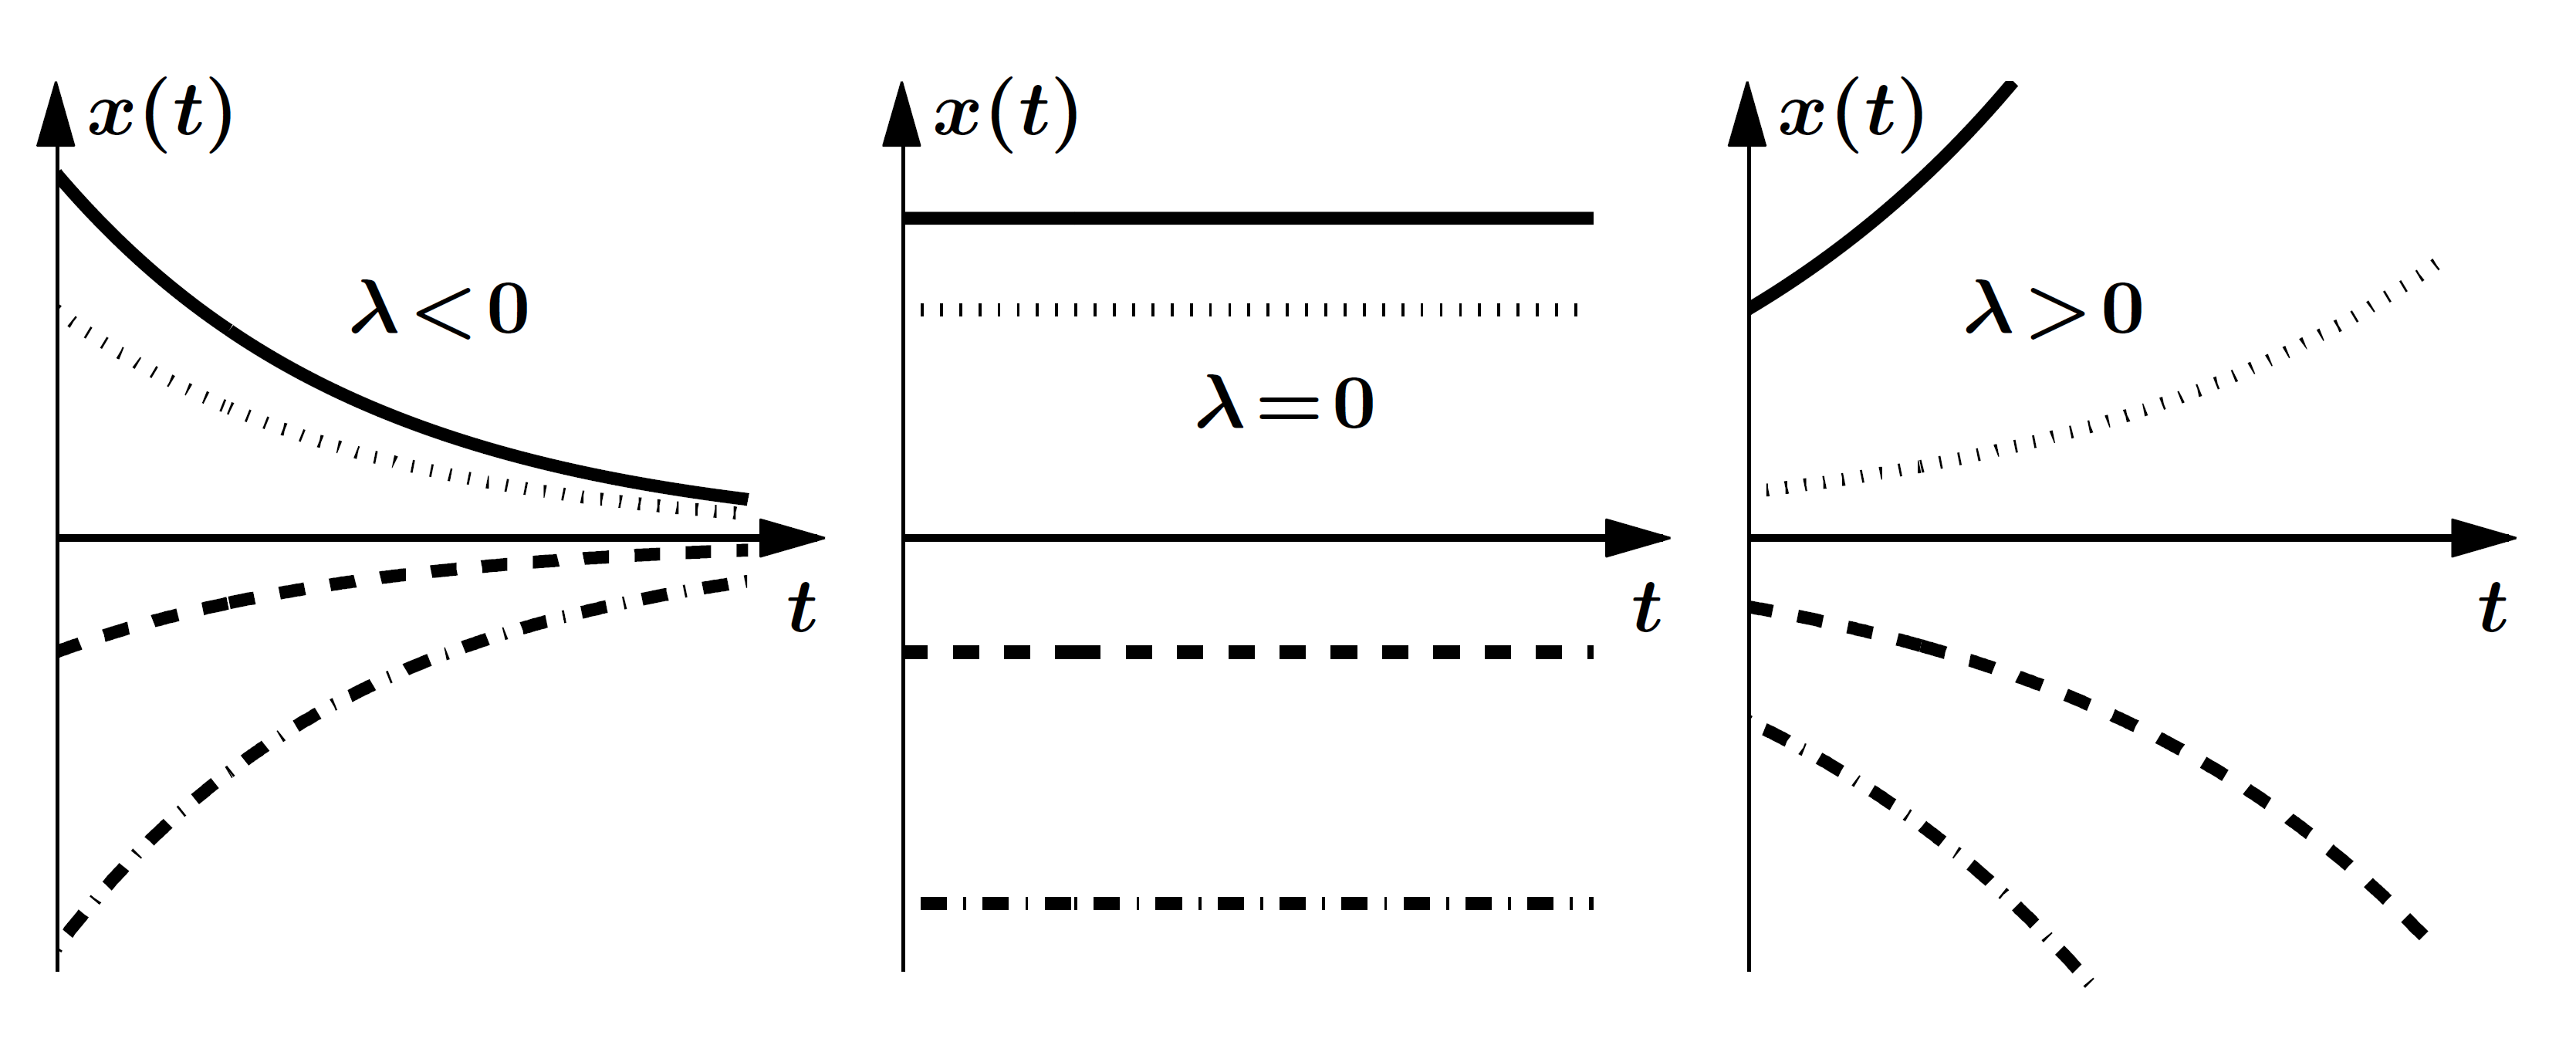
\includegraphics[width=0.5\linewidth]{lin1.png}
  \caption{Solutions $x(t)$ for the equation (\ref{eq:lin1}) for different values of $c$ (solid, dashed, dotted and dash-dotted).}
  \label{fig:lin1}
\end{figure}
If we plot $\dot{x}$ as a function of $x$, we get a {\textbf{phase space}} plot.
The graphs are straight lines given by $\dot{x}=\lambda x$ with a negative, vanishing and positive slope, respectively.
Phase space is one of most important topics in nonlinear dynamics.
\begin{figure}[h!]
  \centering
  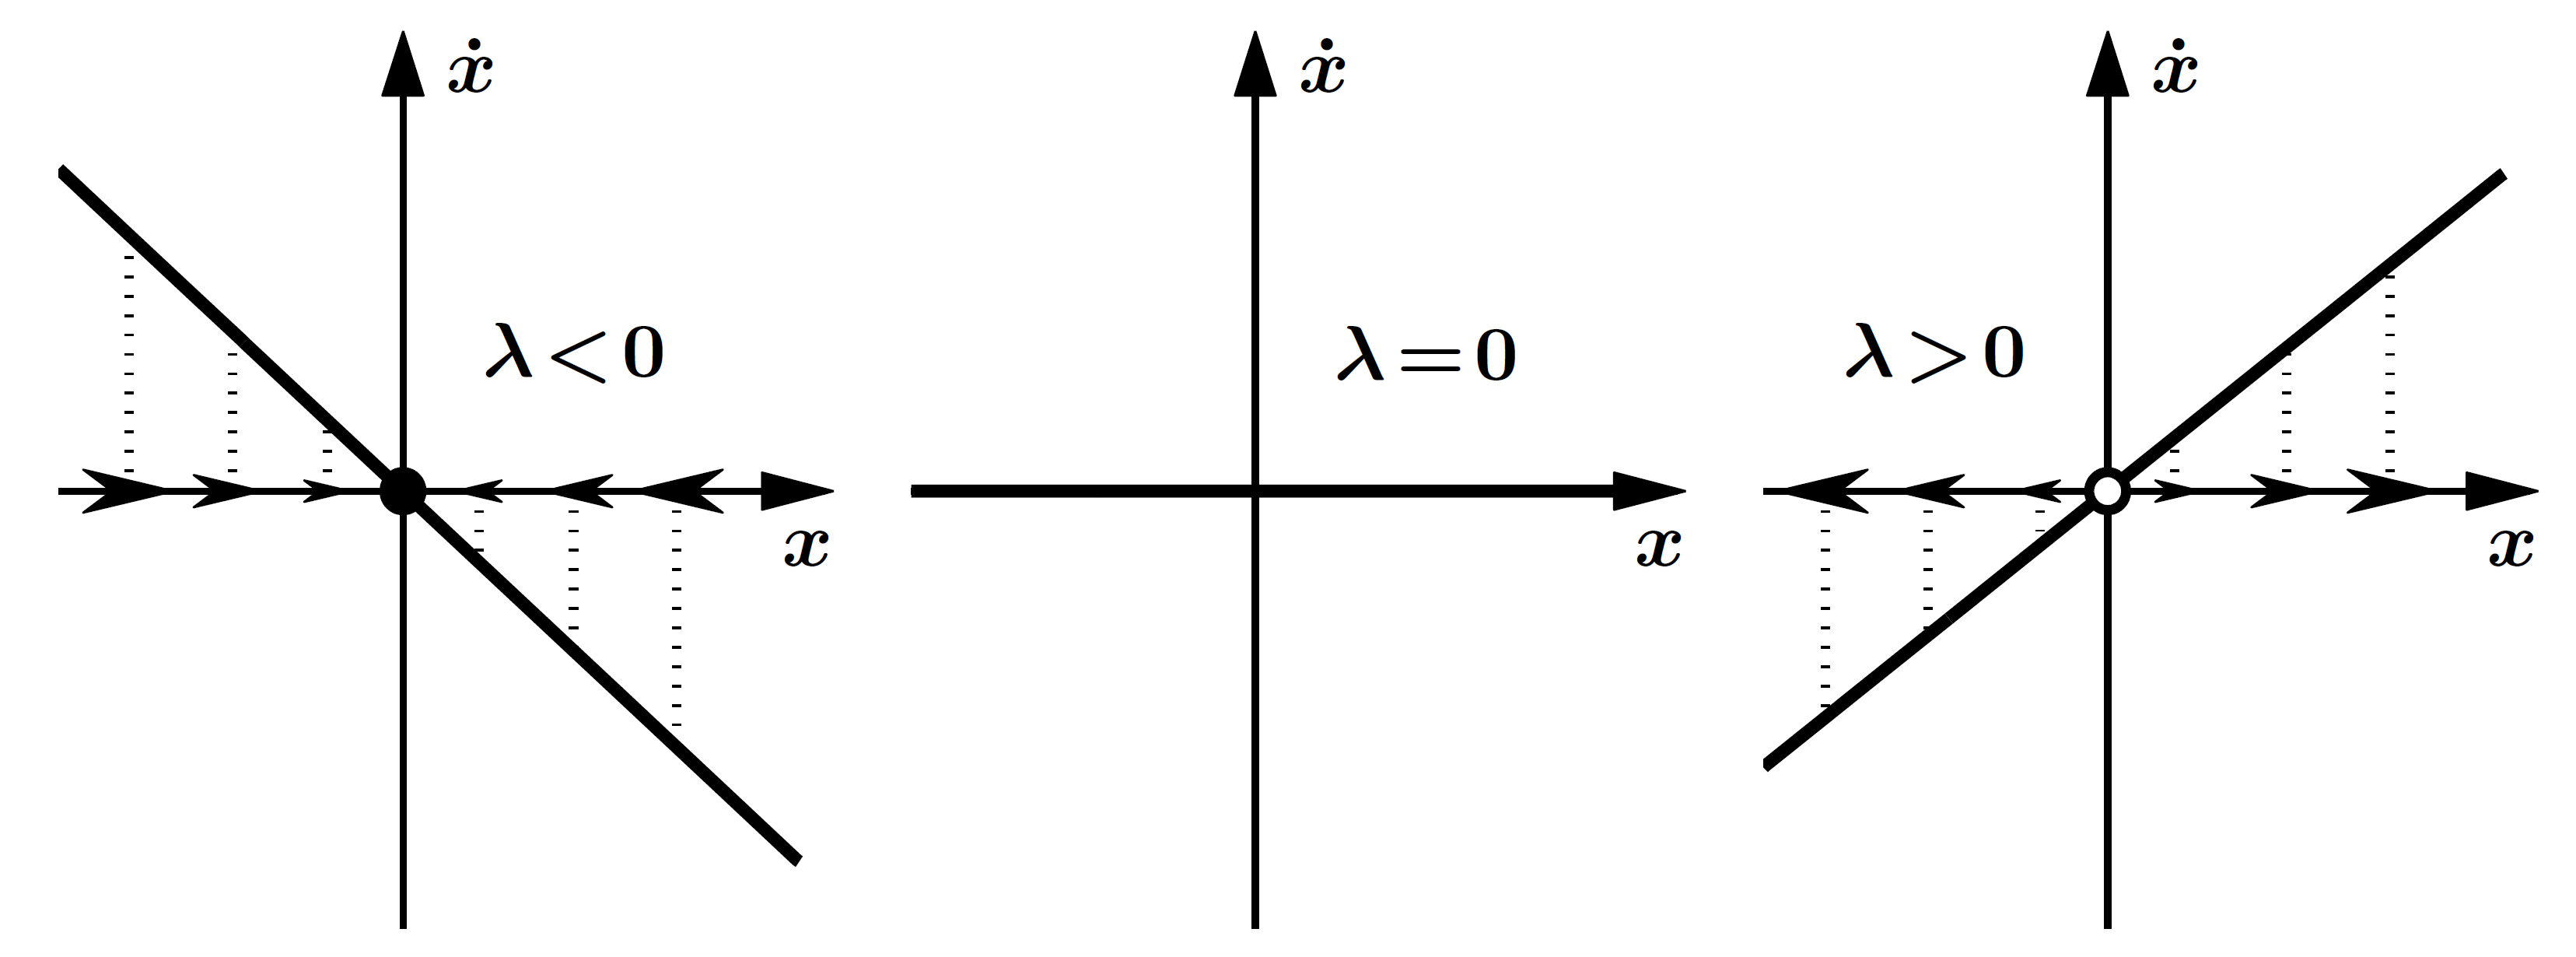
\includegraphics[width=0.5\linewidth]{bps1.png}
  \caption{Phase space plots, $\dot{x}$ as a function of $x$, for the equation (\ref{eq:lin1}).}
  \label{fig:bps1}
\end{figure}
\subsection{Flows on the Line}
Nonlinear Systems are harder to solve analytically, it's even impossible for many cases.
So, we use geometrical approach which gives qualitative behaviour of the system.
Imagine that a fluid is flowing along the real line with a local velocity $f(x)$.
This imaginary fluid is called the {\textbf{phase fluid}}, and the real line is the {\textbf{phase space}}.
The flow is to the right where $f(x)>0$ and to the left where $f(x)<0$.
\emph{Fixed points} have $f(x)=0$.
\begin{figure}[H]
  \centering
  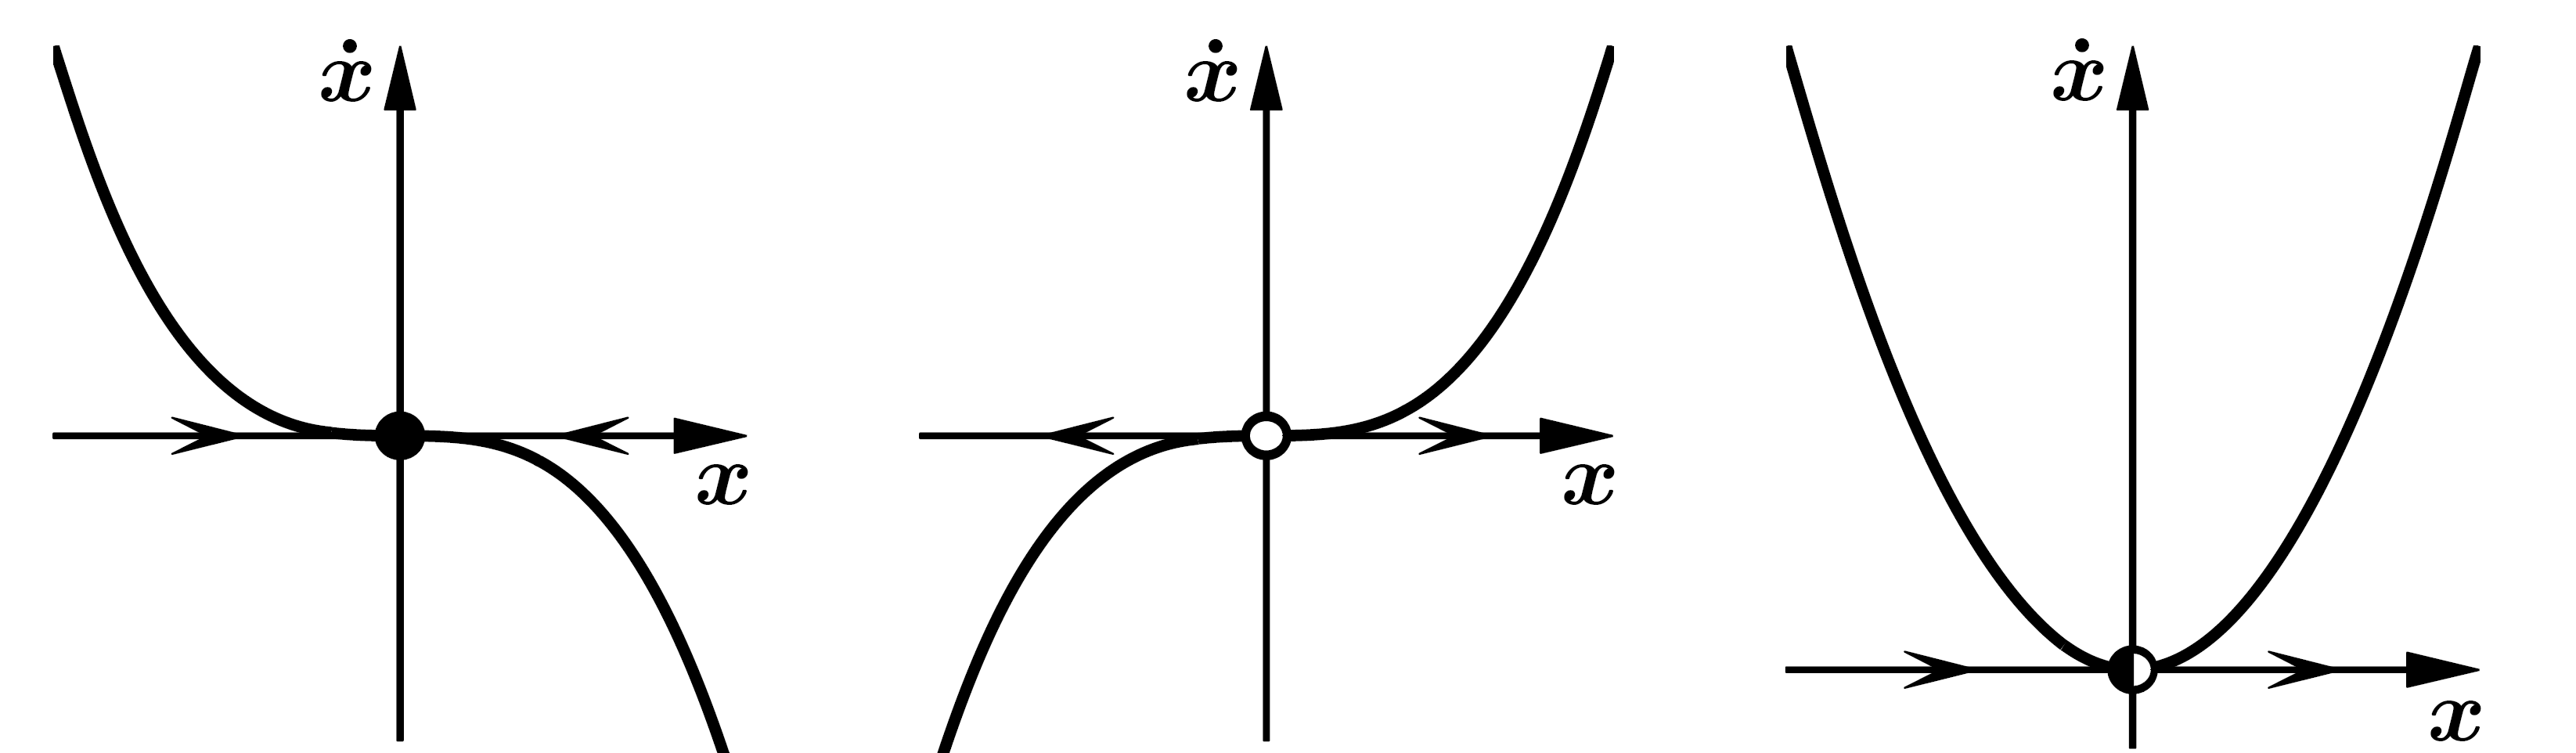
\includegraphics[width=0.5\linewidth]{bfps.png}
  \caption{Phase portrait, solid black dot(left) is a {\textbf{stable}} fixed point (the local flow is toward it) and the open dot(middle) is an {\textbf{unstable}} fixed point (the flow is away from it) and the right one is {\textbf{half-stable}} (the flow is towards it on left and away on right).}
  \label{fig:bfps}
\end{figure}
\subsection{Linear Stability Analysis}
Consider a dynamical system of the form $\dot{x}=f(x)$ and the Taylor expansion around one of its fixed points $\tilde{x}$ and let $\xi=x-\tilde{x}$, then $\dot{\xi}=\dot{x}$
\begin{equation}{\label{eq:lsa1}}
  \dot{x}=f(x) \approx \underbrace{f(\tilde{x})}_{=0}+f^\prime(\tilde{x})\underbrace{(x-\tilde{x})}_{=\xi}+\frac{1}{2!}f^{\prime \prime}(\tilde{x})\underbrace{(x-\tilde{x})^2}_{=\xi^2}+\cdots
\end{equation}
$f(\tilde{x})$ vanishes as it is a fixed point, $|\xi|$ is small as we assume $x$ to be in the vicinity of $\tilde{x}$, and therefore $\xi^2$ is tiny and can be neglected.
Taken together, we obtain an approximation of (\ref{eq:lsa1}) around the fixed point $\tilde{x}$.
\begin{equation}{\label{eq:lsa2}}
  \dot{\xi} = f^\prime(\tilde{x})\ \xi = \lambda\ \xi
\end{equation}
Now, equation (\ref{eq:lsa2}) is similar to equation (\ref{eq:lin1}).
The slope $f^\prime(\tilde{x})$ at the fixed point determines its stability\footnote{Our analysis fails for some $f(x)$ in case where solution is not unique or does not exist, See Theorem (\ref{thm:eut}).}, if $f^\prime(\tilde{x})>0$ then $\tilde{x}$ is a \emph{unstable fixed point} and if $f^\prime(\tilde{x})<0$ then $\tilde{x}$ is a \emph{stable fixed point}.
$1/f^\prime(\tilde{x})$ is a {\textbf{characteristic time scale}}, it determines the time required for $x(t)$ to vary significantly in the neighborhood of $\tilde{x}$.
\subsection{Potential Functions}{\label{sec:pf}}
A second way of representing the dynamics of such systems graphically is the landscape defined by its \emph{potential function}.
The potential of a dynamical system is a function $V(x)$ such that the relation
\begin{equation}
  \dot{x}=f(x)= -\frac{dV(x)}{dx}
\end{equation}
is fulfilled.
All one-dimensional systems have a potential function.\\
As time evolves, either the value of the potential function decreases, or it stays constant if a local or global minimum of $V(x)$ has been reached.
This behavior can easily be seen by calculating the derivative of $V$ with respect to time
\begin{equation}
  \dot{V}=\frac{dV(x)}{dt}=\underbrace{\frac{dV}{dx}}_{-\dot{x}}\underbrace{\frac{dx}{dt}}_{\dot{x}}=-\left\{\frac{dV}{dx}\right\}^2=-\dot{x}^2\leq0
\end{equation}
Local \emph{minima} of $V$ correspond to {\textbf{stable}} fixed points, local \emph{maxima} correspond to {\textbf{unstable}} fixed points, {\textbf{half-stable}} fixed points are found at locations where the tangent at an \emph{inflection point} is horizontal.
\subsubsection{Impossibility of Oscillations}
Fixed points dominate the dynamics of first-order systems.
Trajectories either approach a fixed point, or diverged to $\pm\infty$.
The reason is that trajectories are forced to increase or decrease monotonically, or remain constant.
If a fixed point is regarded as an equilibrium solution, the approach to equilibrium is always monotonic-overshoot and damped oscillations can never occur in a first-order system.
Hence there are no periodic solutions to $\dot{x}=f(x)$.
\subsection{Flows on the Circle}
Periodic systems can be realized in one dimension with dynamics that take place not on a line but on a circle.
The state variable here is not $x$, it is $\theta$ with $0\leq\theta<2\pi$ or $-\pi\leq\theta<\pi$.
The general form here is
\begin{equation}
  \dot{\theta}=f(\theta)\ \text{with}\ f(\theta+2\pi)=f(\theta)
\end{equation}
The function $f(\pi)$ has to be $2\pi-$periodic to ensure that it has the same value at $\theta=0$ and $\theta=2\pi$, which are the same points.
\subsubsection{Nonuniform Oscillator}{\label{sec:nuo}}
It has the equation
\begin{equation}
  \dot{\theta}=\omega-a\sin\theta
\end{equation}
The parameter $a$ introduces a nonuniformity in the flow around the circle, the flow is fastest at $\theta=-\pi/2$ and slowest at $\theta=\pi/2$.
\begin{figure}[H]
  \centering
  \begin{subfigure}{0.45\linewidth}
    \centering
    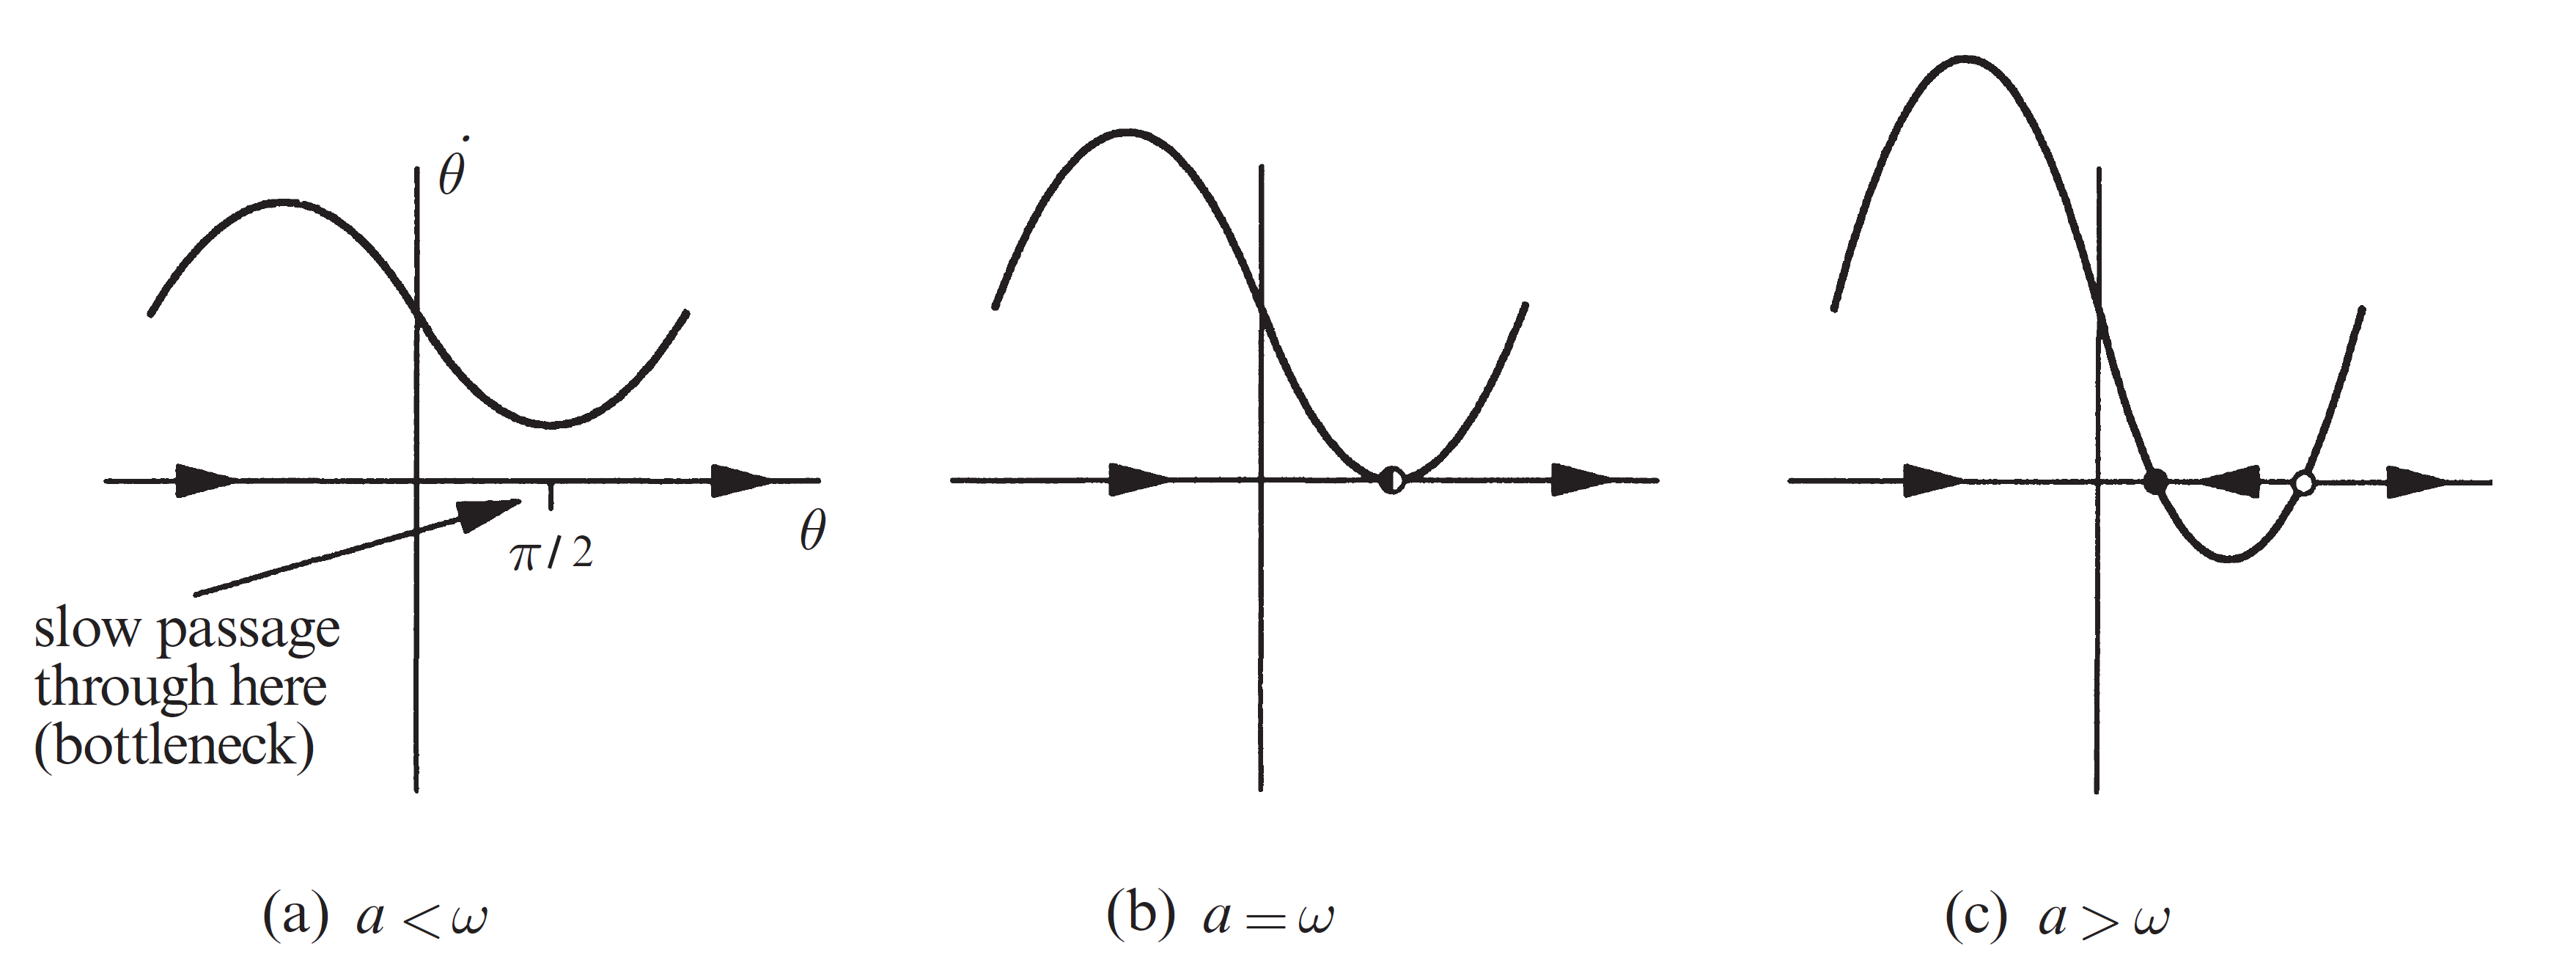
\includegraphics[width=\linewidth]{fotc1.png}
    \caption{}
    \label{fig:fotc1}
  \end{subfigure}
  \vline
  \begin{subfigure}{0.45\linewidth}
    \centering
    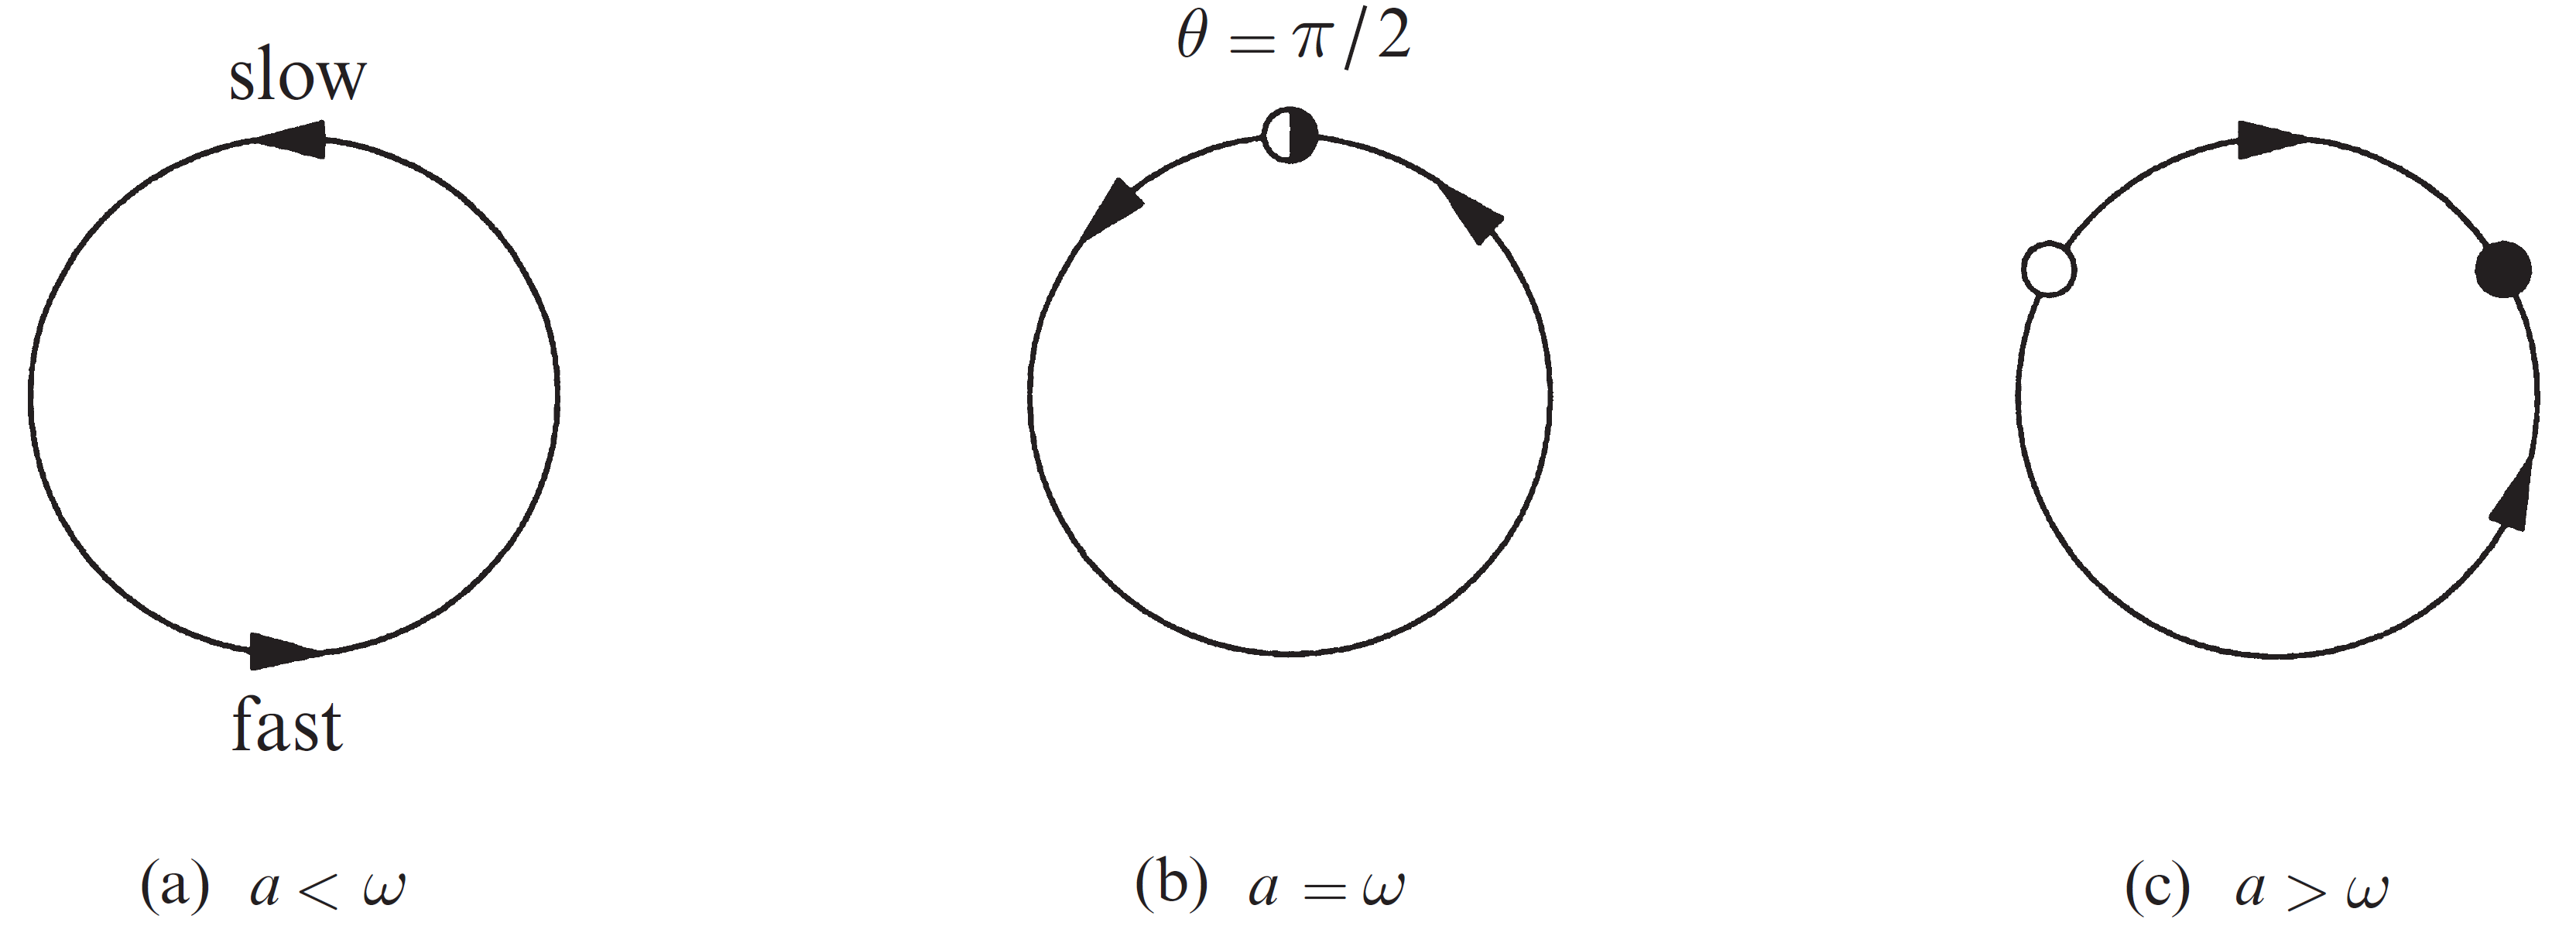
\includegraphics[width=\linewidth]{fotc2.png}
    \caption{}
    \label{fig:fotc2}
  \end{subfigure}
  \caption{}
\end{figure}
\begin{itemize}
  \item For $a<\omega$, the period of the oscillation\footnote{$$T=\int dt=\int_0^{2\pi} \frac{dt}{d\theta}d\theta=\int_0^{2\pi}\frac{d\theta}{\omega-a\sin\theta}$$} $T=\dfrac{2\pi}{\sqrt{\omega^2-a^2}}$.
  \item When $a$ is slightly less than $\omega$, the oscillation is very jerky: the phase point $\theta(t)$ takes a long time to pass through a \emph{bottleneck} near $\theta=\pi/2$, after which it zips around the rest of the circle on a much faster time scale (Figure (\ref{fig:fotc1}a)).
  \item When $a=\omega$, the system stops oscillating altogether: a half-stable fixed point has been born in a saddle-node bifurcation (See Section ({\ref{sec:snbf}})) at $\theta=\pi/2$ (Figure (\ref{fig:fotc1}b)).
  \item Finally, when $a>\omega$, the half-stable fixed point splits into a stable and unstable fixed point (Figure (\ref{fig:fotc1}c)).
  All trajectories are attracted to the stable fixed point as $t\rightarrow\infty$.
\end{itemize}
The same information can be shown by plotting the vector fields on the circle (Figure (\ref{fig:fotc2})).
\begin{comment}
\begin{figure}[H]
  \centering
  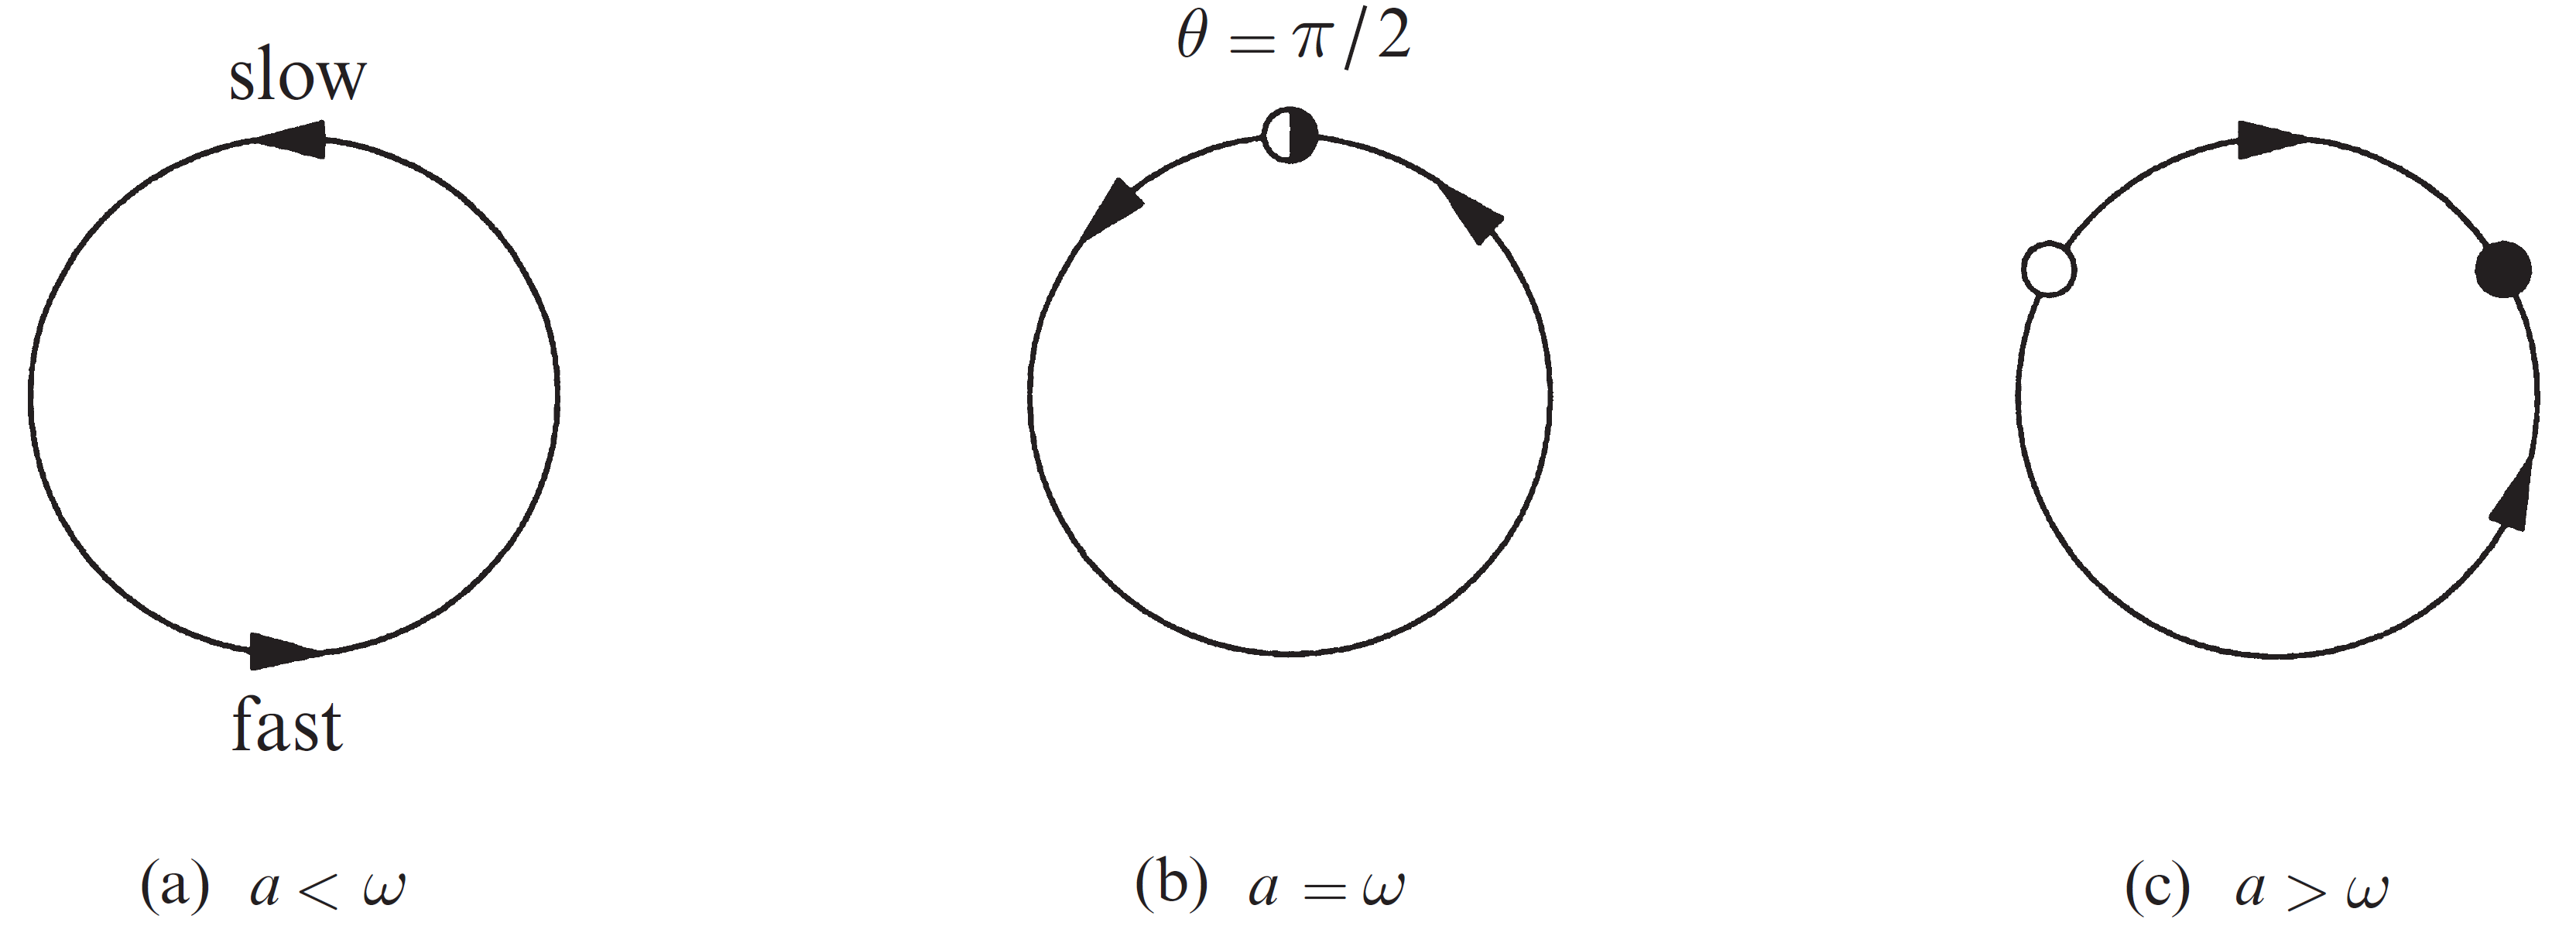
\includegraphics[width=0.5\linewidth]{fotc2.png}
  \caption{}
  \label{fig:fotc2}
\end{figure}
\end{comment}

\section{Bifurcations}
One important property of nonlinear systems is their ability to undergo qualitative changes in their dynamical behavior when a parameter exceeds a critical value.
It is possible to display the locations and stability of fixed points as a function of the parameter in a single plot called a \emph{bifurcation\footnote{See definition at Section (\ref{sec:bf2d})} diagram}.
In these diagrams the locations of stable fixed points are represented by solid lines, unstable fixed points are shown dashed.
Also, solid, open and half-filled circles are used to mark stable, unstable and half-stable fixed points, respectively.
\subsection{Local Bifurcations}
A local bifurcation occurs when a parameter change causes the stability of an equilibrium (or fixed point) to change. See Section (\ref{sec:lb}) for detailed discussion.
\subsubsection{Saddle-Node Bifurcation}{\label{sec:snbf}}
The prototype of a system that undergoes a saddle-node bifurcation is given by
\begin{equation}{\label{eq:snbf}}
  \dot{x}=\lambda+x^2 \quad \rightarrow \quad \tilde{x}_{1,2}=\pm\sqrt{-\lambda}
\end{equation}
The graph in phase space for (\ref{eq:snbf}) is a parabola that opens upwards (Figure (\ref{fig:snbf})).
For negative values of $\lambda$ one stable and one unstable fixed point exist, which collide and annihilate when $\lambda$ is increased above zero.
There are no fixed points in this system for positive values of $\lambda$.
\begin{figure}[h!]
  \centering
  \begin{subfigure}{0.45\linewidth}
    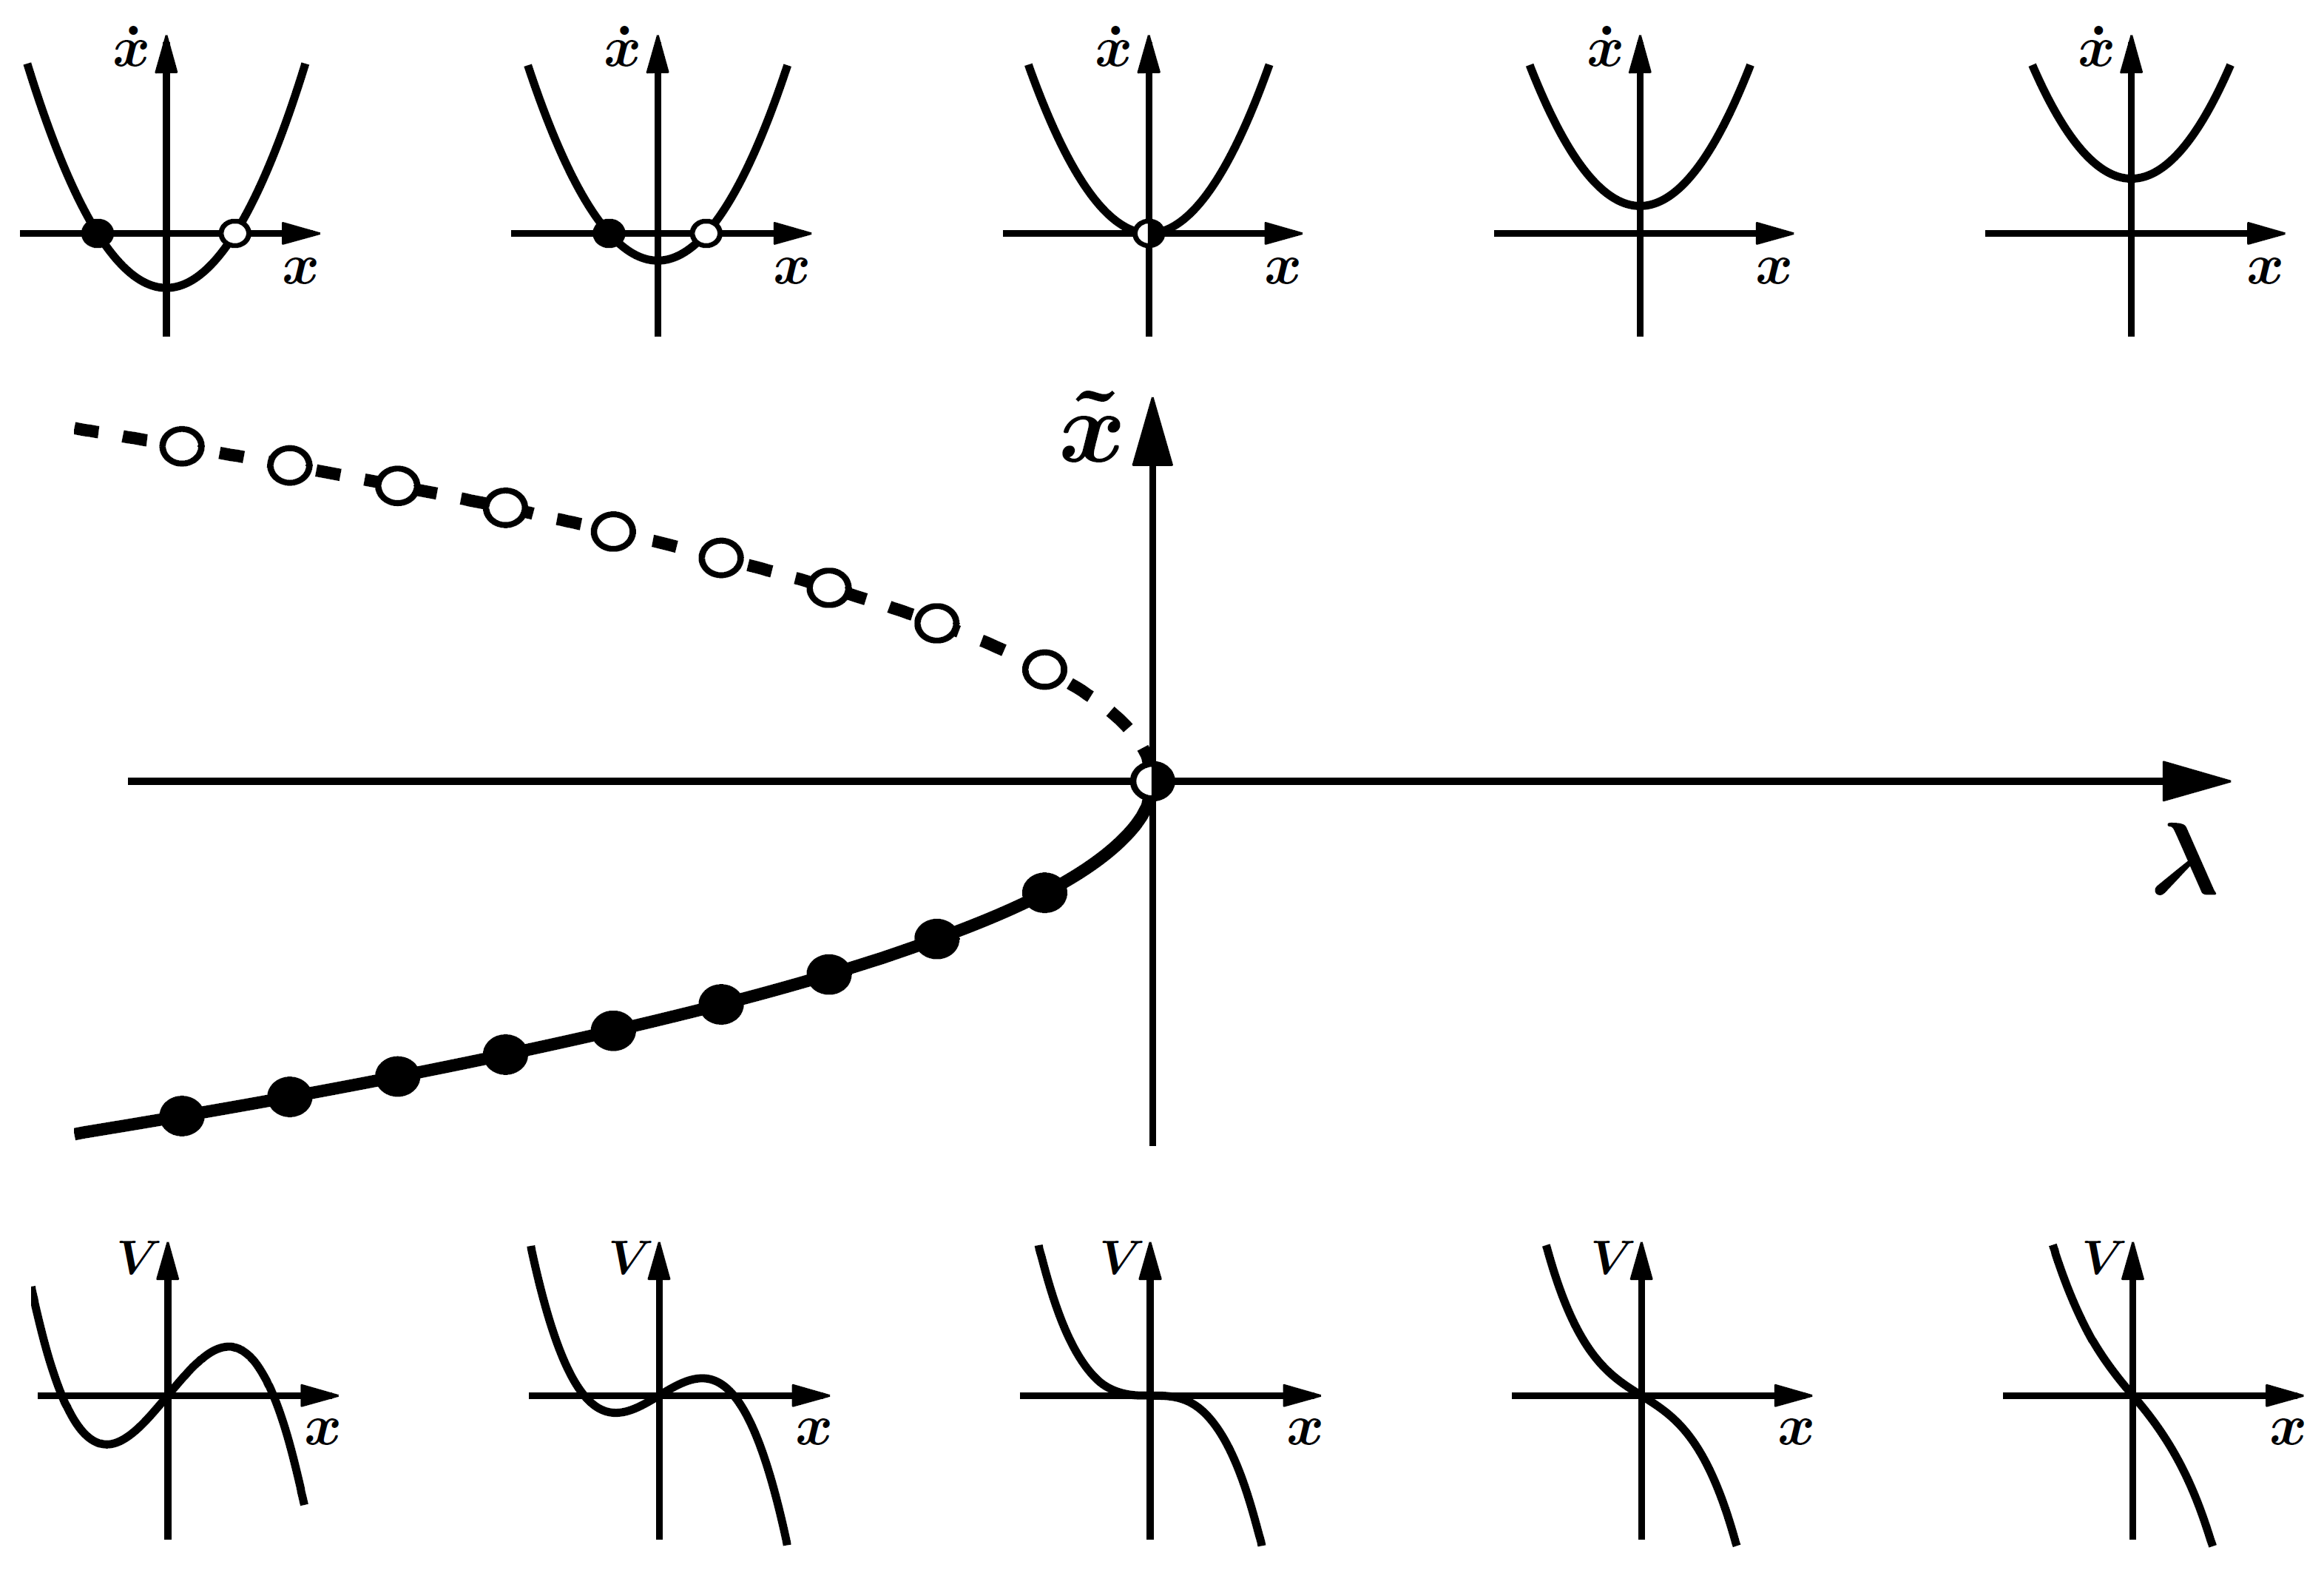
\includegraphics[width=\linewidth]{snbf.png}
    \caption{Saddle-node bifurcation.}
    \label{fig:snbf}
  \end{subfigure}
  \vline
  \begin{subfigure}{0.45\linewidth}
    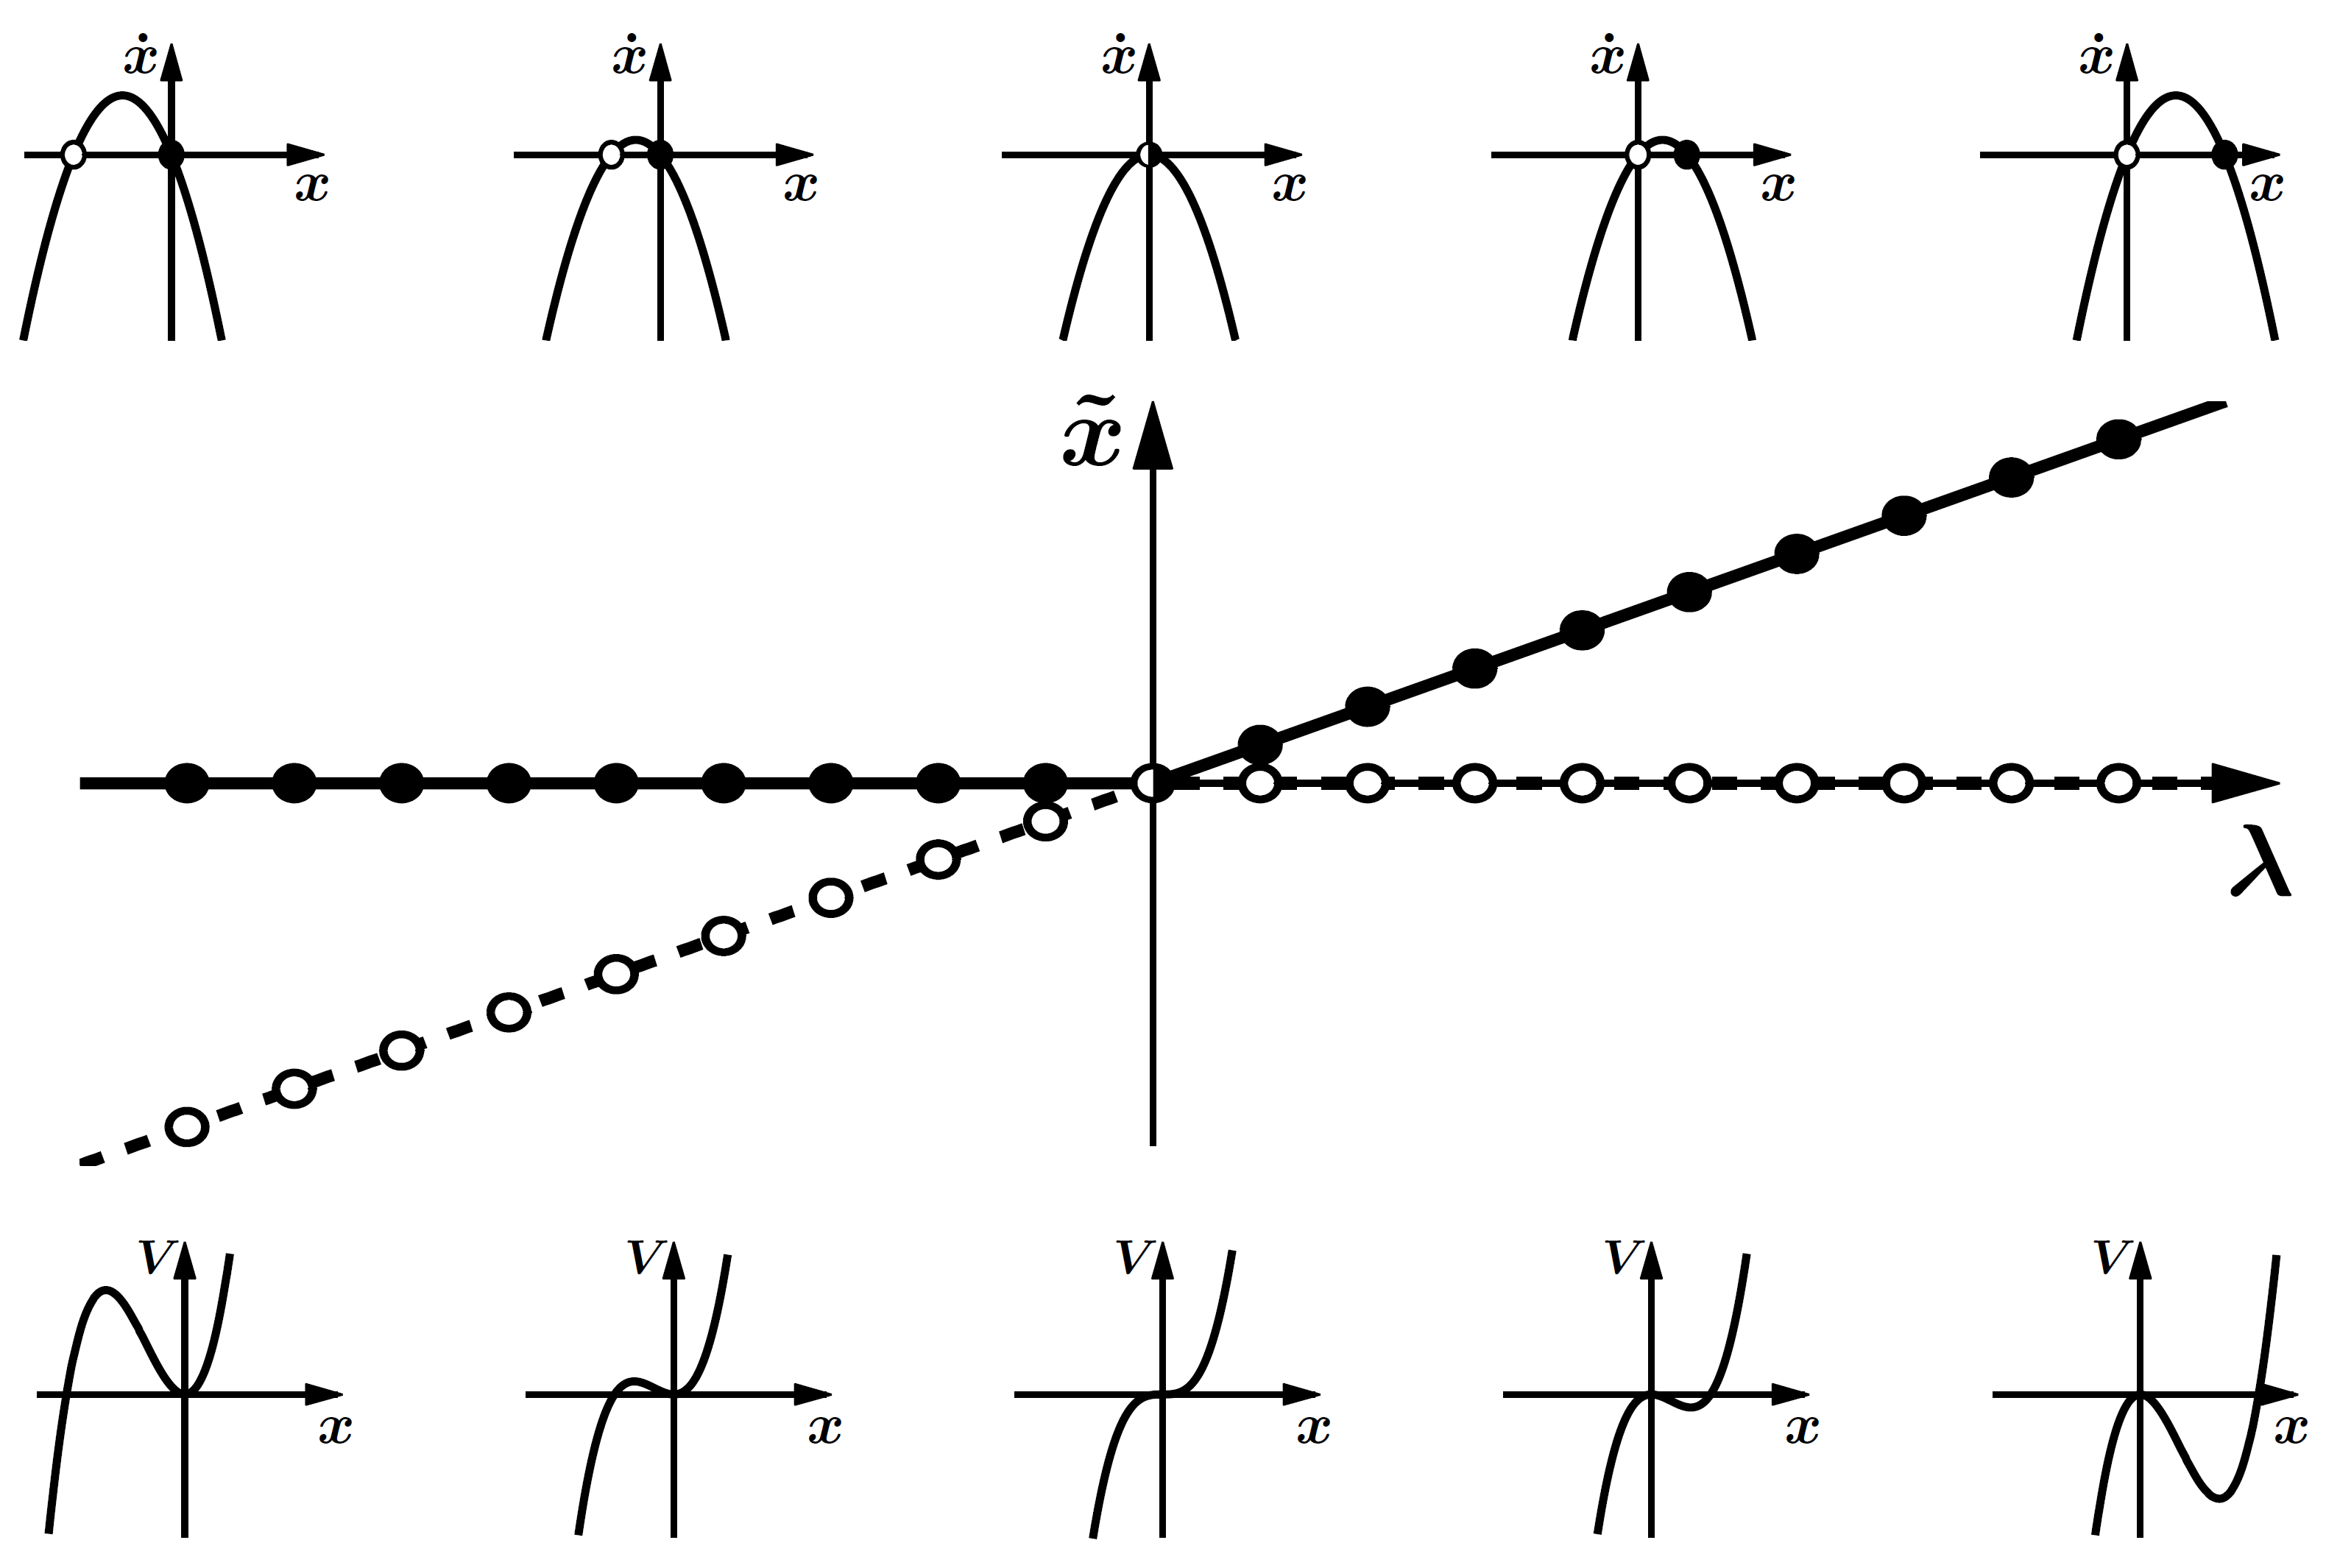
\includegraphics[width=\linewidth]{tbf.png}
    \caption{Transcritical bifurcation.}
    \label{fig:tbf}
  \end{subfigure}
  \caption{Top: phase space plots; middle: bifurcation diagram; bottom: potential functions.}
  \label{fig:stbf}
\end{figure}
\subsubsection{Transcritical Bifurcation}
The transcritical bifurcation is given by
\begin{equation}{\label{eq:tbf}}
  \dot{x}=\lambda x-x^2 \quad \rightarrow \quad \tilde{x}_1=0, \tilde{x}_2=\lambda
\end{equation}
The system has a stable and an unstable fixed point for all values except for $\lambda=0$ (Figure (\ref{fig:tbf})).
The bifurcation diagram consists of two straight lines, one given by $\tilde{x}=0$ and one with a slope of one.
When these lines intersect at the origin the fixed points they \emph{exchange stability}.
\subsubsection{Supercritical Pitchfork Bifurcation}{\label{sec:spcpbf}}
The supercritical pitchfork bifurcation is visualized in Figure (\ref{fig:spbf}) and prototypically given by
\begin{equation}{\label{eq:spbf}}
  \dot{x}=\lambda x- x^3 \quad \rightarrow \quad \tilde{x}_1=0, \tilde{x}_{2,3}=\pm\sqrt{\lambda}
\end{equation}
A single stable fixed point at the origin becomes unstable and a pair of stable fixed points appears symmetrically around $\tilde{x}=0$.
In terms of symmetry this system has an interesting property: the equation(\ref{eq:spbf}) is invariant if we substitute $x$ by $-x$.
All phase plots have a point symmetry with respect to the origin and the plots of the potential have a mirror symmetry with respect to the vertical axis (Figure (\ref{fig:spbf})).
When $\lambda>0$, the slightest perturbation will move the ball to the left or right where the slope is finite and it will settle down in one of the new minima as in Figure (\ref{fig:spbf})(bottom right).
This phenomenon is called \emph{spontaneous symmetry breaking}.
\begin{figure}[h!]
  \centering
  \begin{subfigure}{0.45\linewidth}
    \centering
    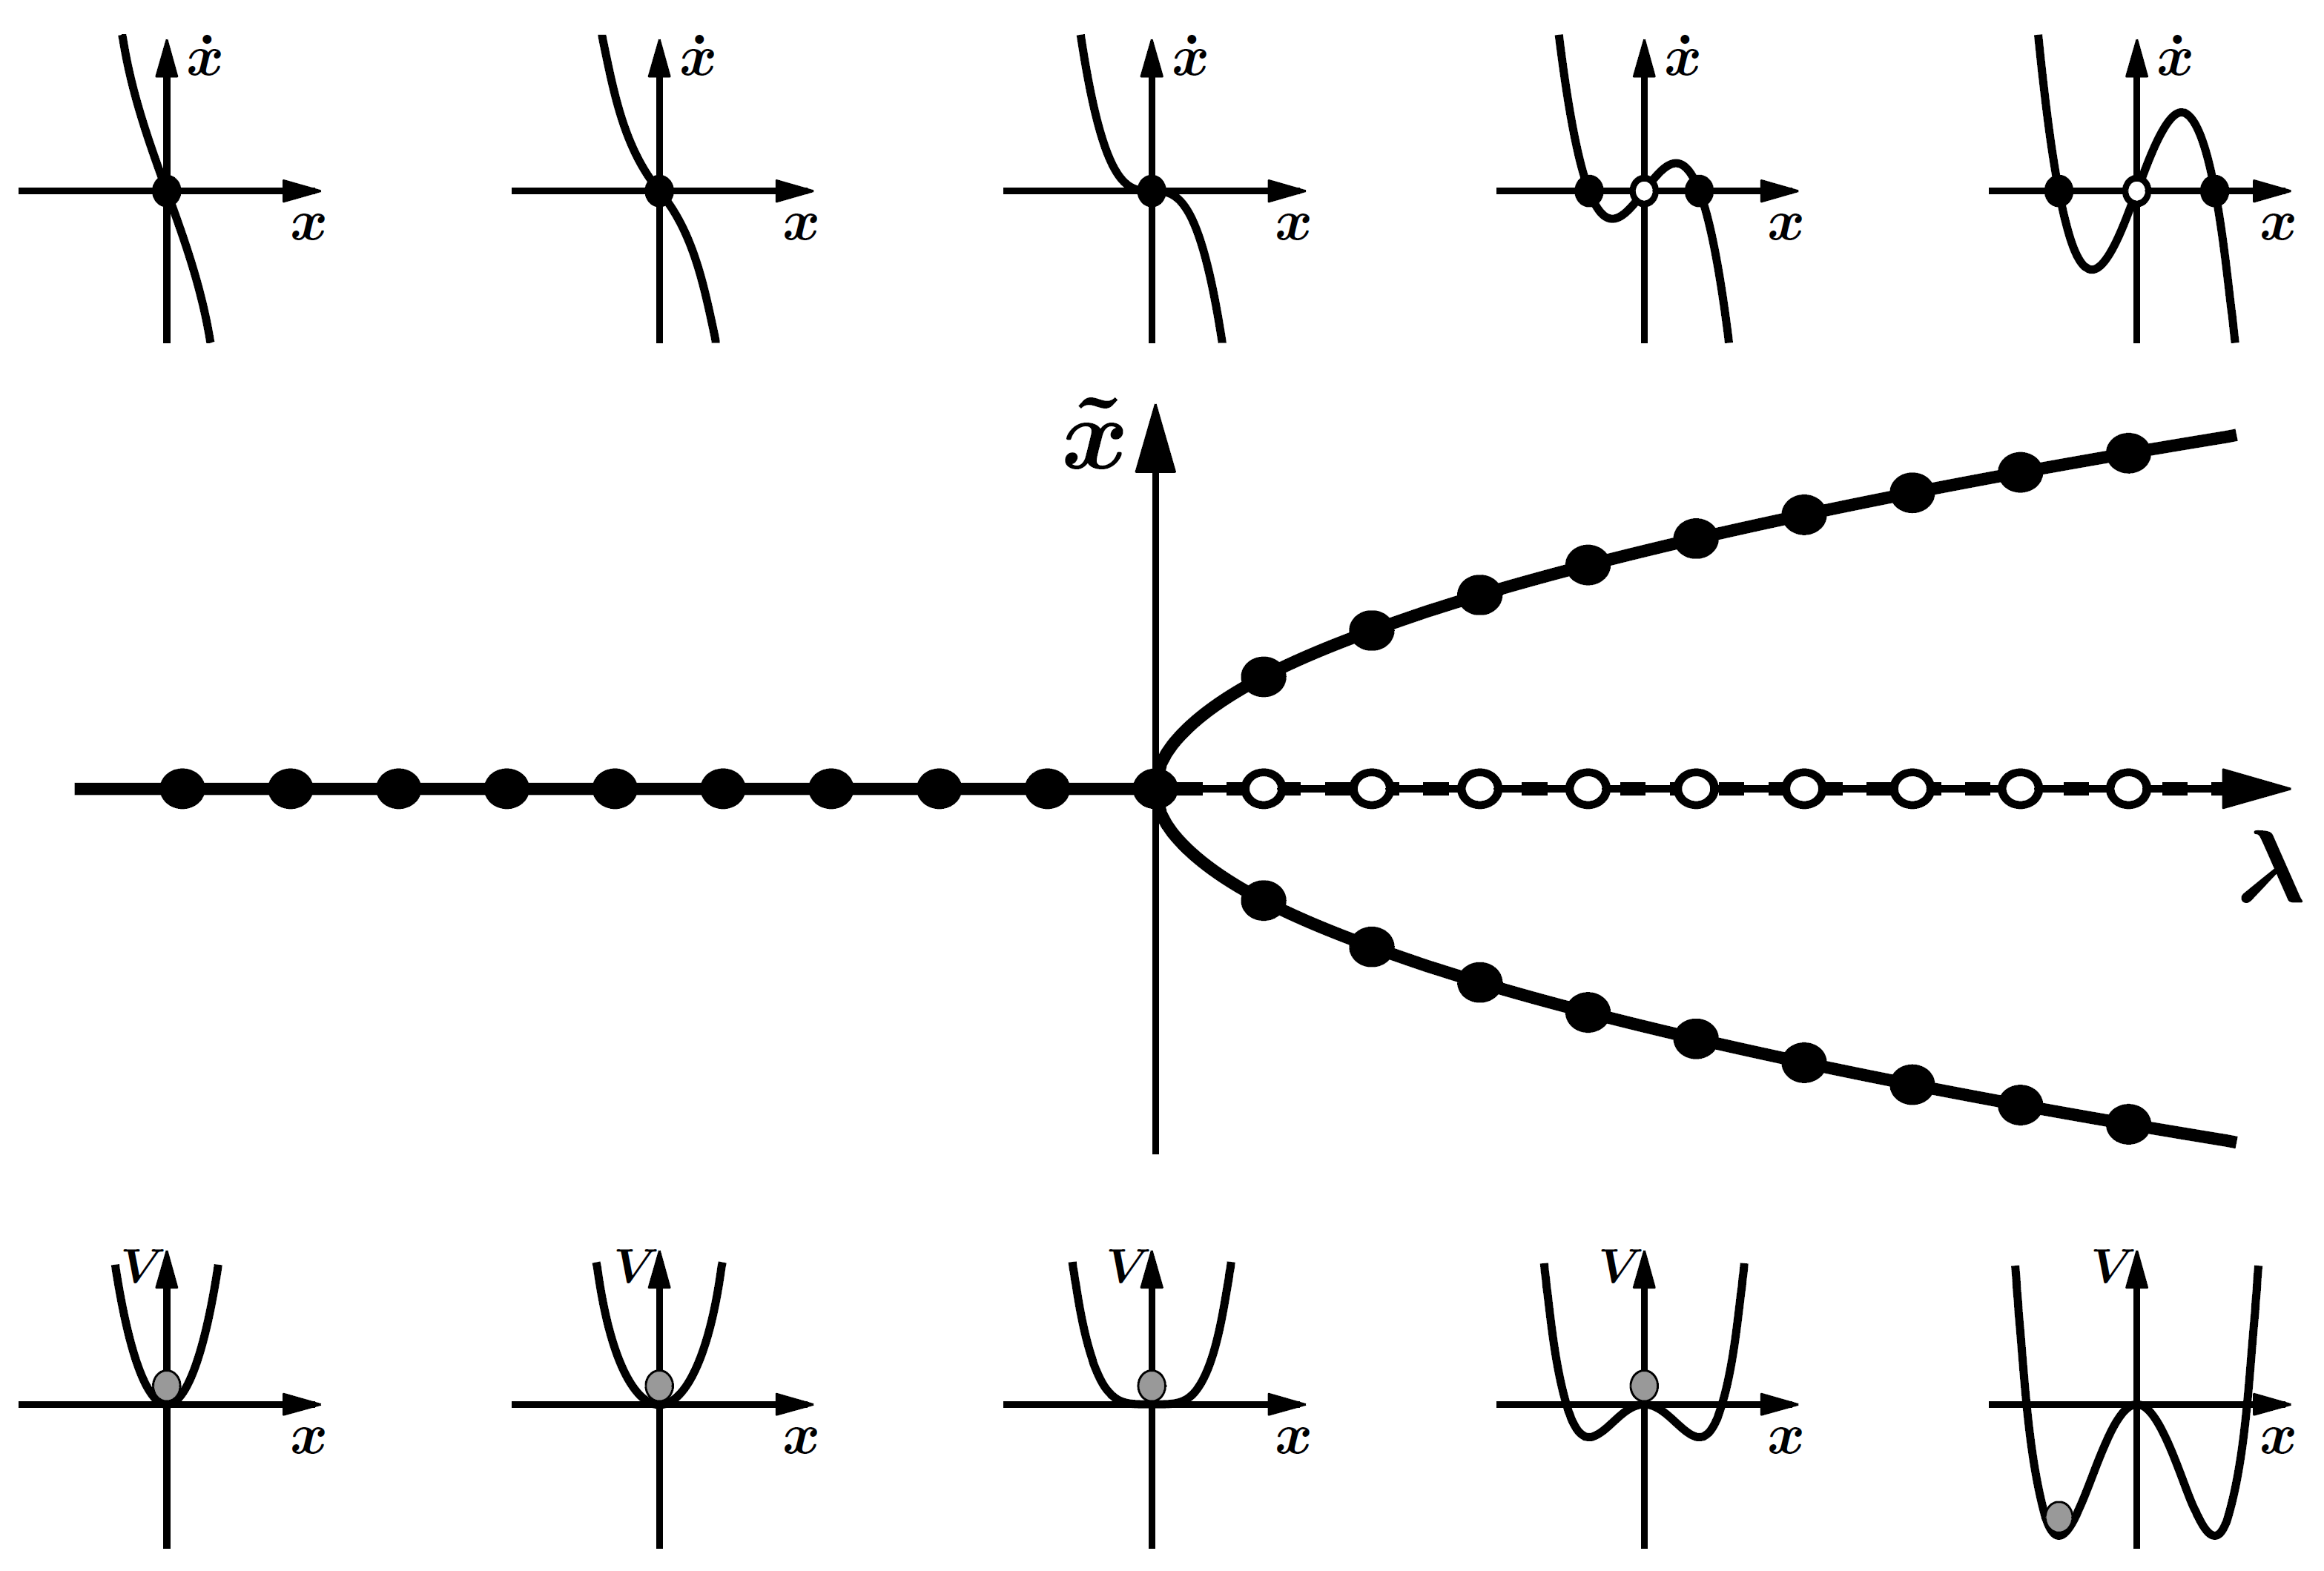
\includegraphics[width=\linewidth]{spbf.png}
    \caption{Supercritical Pitchfork bifurcation.}
    \label{fig:spbf}
  \end{subfigure}
  \vline
  \begin{subfigure}{0.45\linewidth}
    \centering
    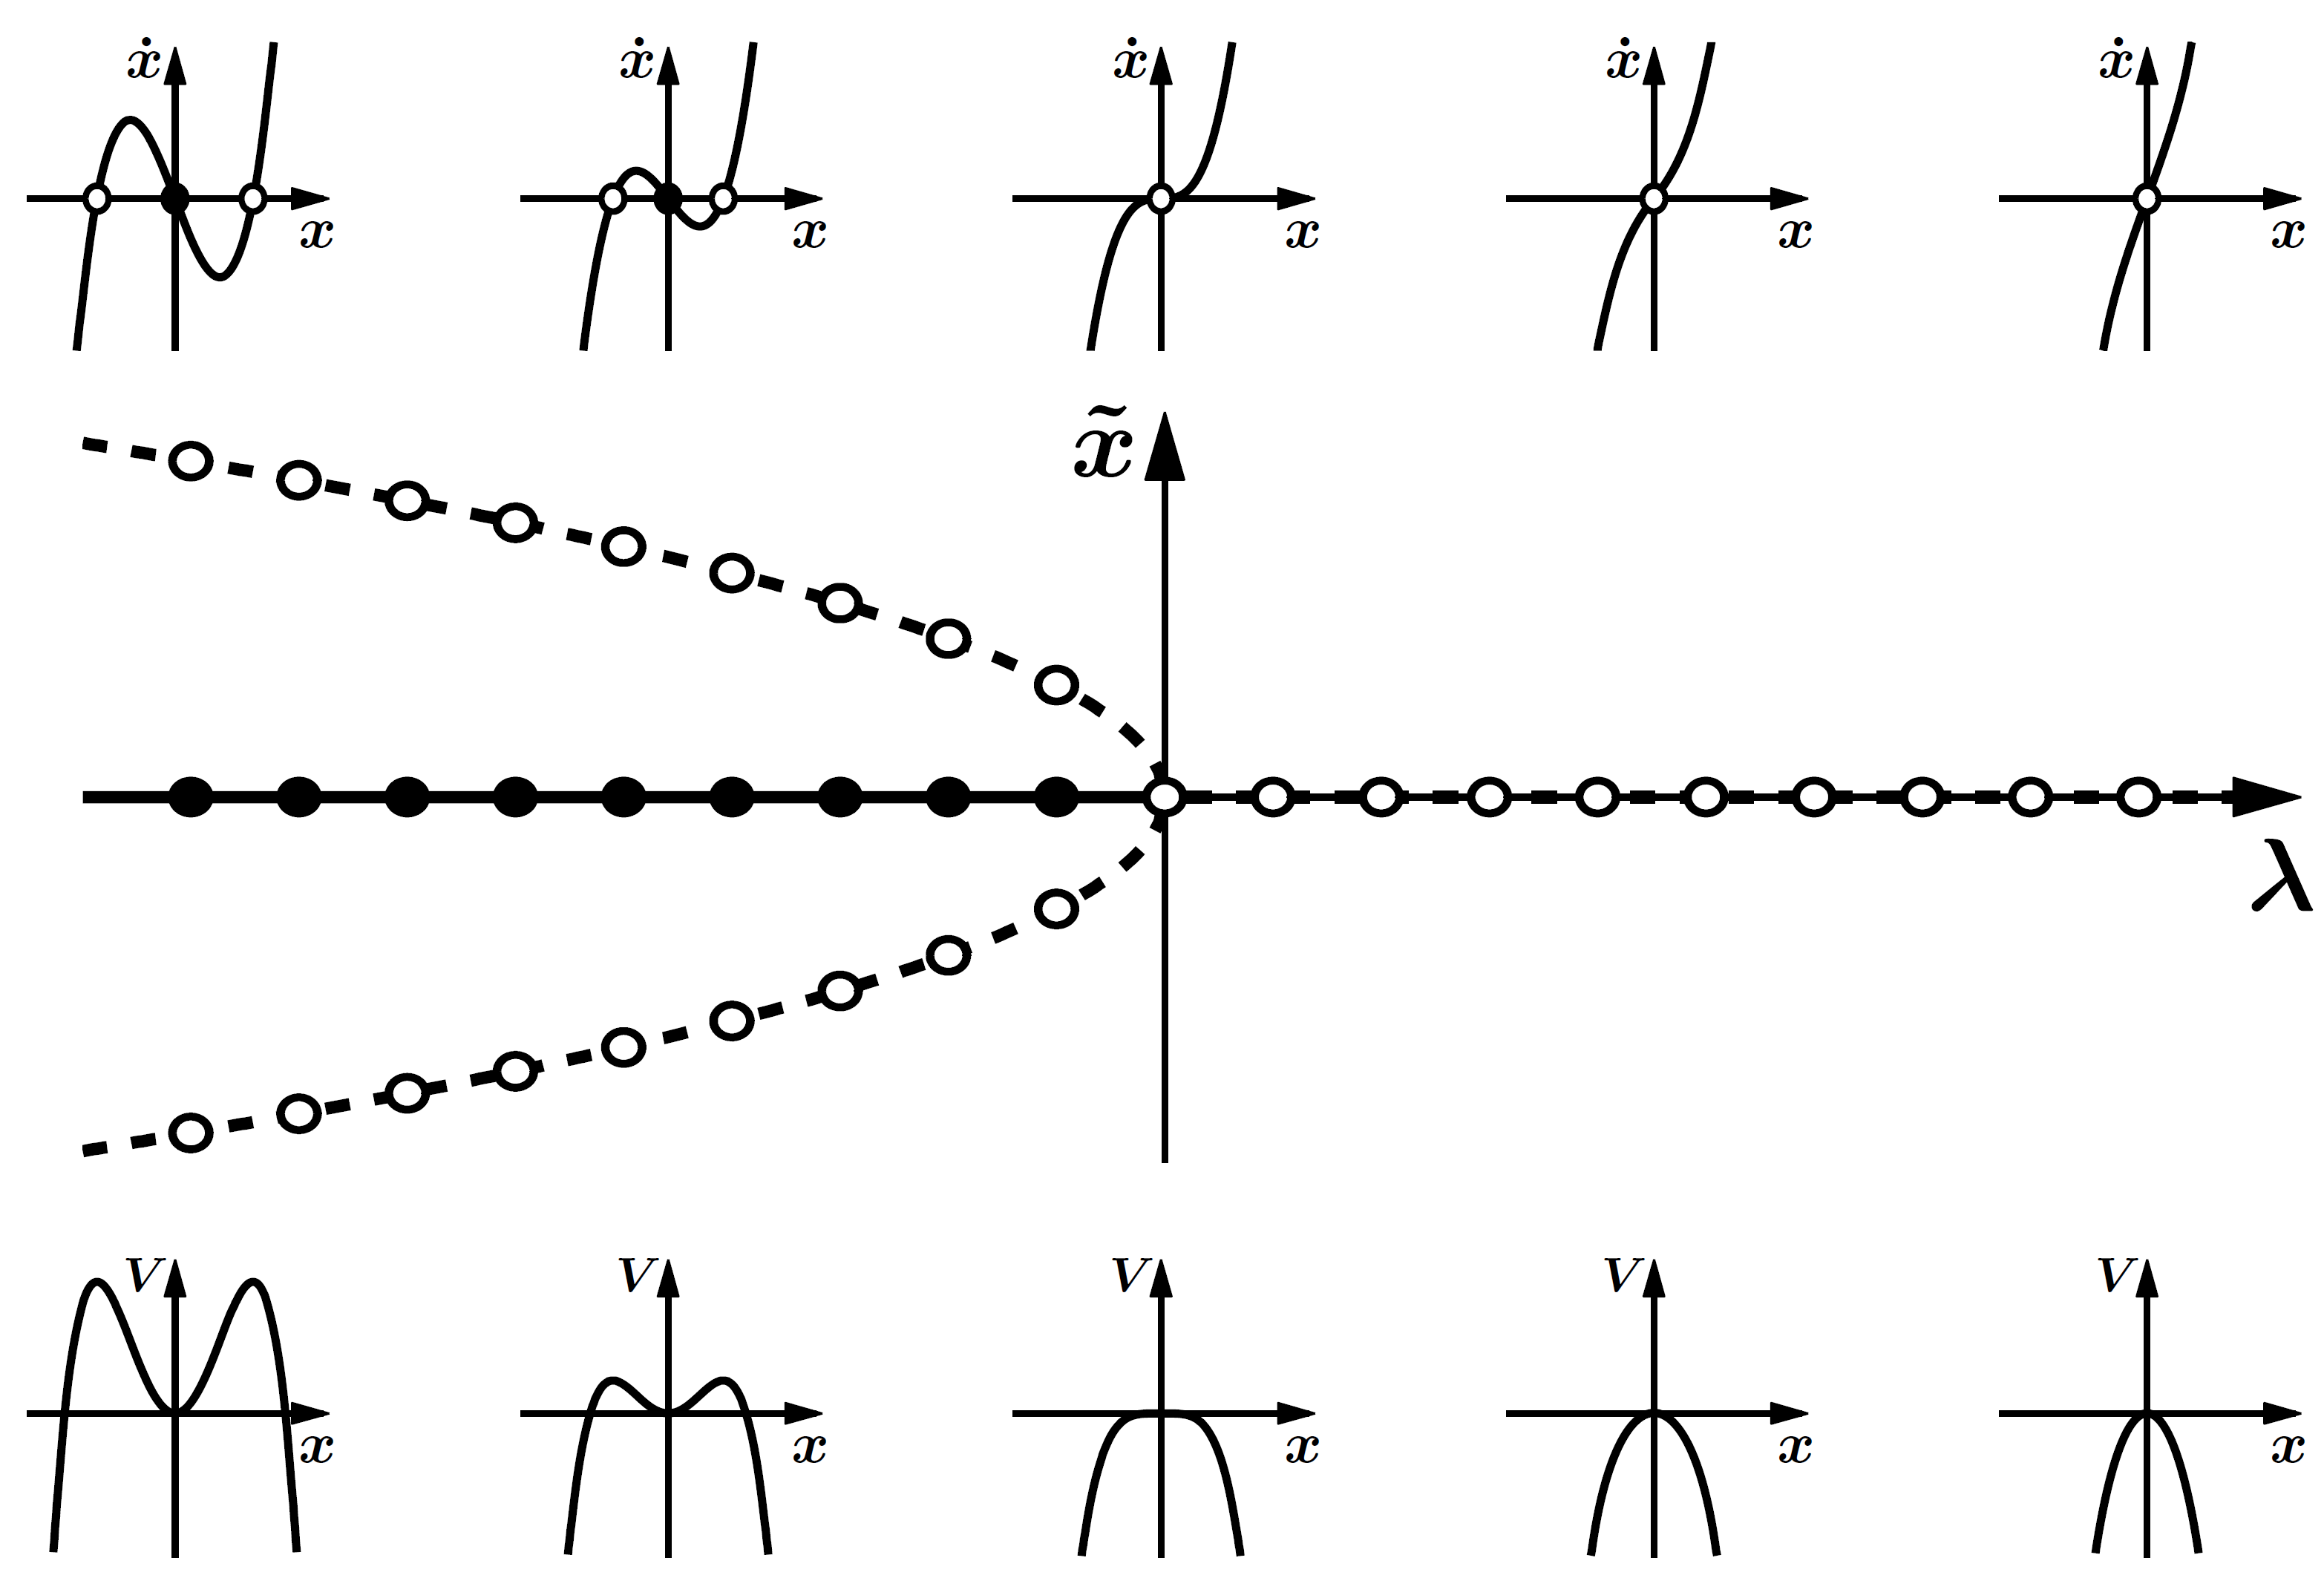
\includegraphics[width=\linewidth]{sbbf.png}
    \caption{Subcritical Pitchfork bifurcation.}
    \label{fig:sbbf}
  \end{subfigure}
  \caption{Top: phase space plots; middle: bifurcation diagram; bottom: potential functions.}
  \label{fig:sbf}
\end{figure}
\subsubsection{Subcritical Pitchfork Bifurcation}
The equation governing the subcritical pitchfork bifurcation is given by
\begin{equation}\label{eq:sbbf}
  \dot{x}=\lambda x+ x^3 \quad \rightarrow \quad \tilde{x}_1=0, \tilde{x}_{2,3}=\pm\sqrt{-\lambda}
\end{equation}
As in the supercritical case, the origin is stable for negative values of $\lambda$ and becomes unstable when the parameter exceeds $\lambda =0$ (Figure (\ref{fig:sbbf})).
Two additional fixed points exist for negative parameter values of $\lambda$ at $\tilde{x}=\pm\sqrt{-\lambda}$ and they are both repellers.
\begin{theorem}[\textbf{Bifurcations}]
  Suppose the system $\dot{x}(t)=f(x,\lambda), x,\lambda\in\mathbb{R}$ has an equilibrium point $x=x_0$ at $\lambda=\lambda_0$ satisfying the conditions
  \begin{equation}
    f(x_0,\lambda_0)=0\qquad\frac{\partial f}{\partial x}(x_0,\lambda_0)=0
  \end{equation}
  \begin{itemize}
    \item
    \begin{equation}
      \frac{\partial f}{\partial \lambda}(x_0,\lambda_0)\neq0\quad\frac{\partial^2 f}{\partial x^2}(x_0,\lambda_0)\neq0
    \end{equation}
    The system has a saddle-node bifurcation at $(x_0,\lambda_0)$.
    \item
    \begin{equation}
      \frac{\partial f}{\partial \lambda}(x_0,\lambda_0)=0\quad\frac{\partial^2 f}{\partial x^2}(x_0,\lambda_0)\neq0\quad\frac{\partial^2f}{\partial x\partial y}(x_0,\lambda_0)\neq0
    \end{equation}
    The system has a transcritical bifurcation at $(x_0,\lambda_0)$.
    \item
    \begin{equation}
      \frac{\partial f}{\partial \lambda}(x_0,\lambda_0)=0\quad\frac{\partial^2 f}{\partial x^2}(x_0,\lambda_0)=0\quad\frac{\partial^2f}{\partial x\partial y}(x_0,\lambda_0)\neq0\quad\quad\frac{\partial^3f}{\partial x^3}(x_0,\lambda_0)\neq0
    \end{equation}
    The system has a pitchfork bifurcation at $(x_0,\lambda_0)$.
  \end{itemize}
\end{theorem}
\subsection{Bifurcations and Hysteresis}
In equation, 
\begin{equation}
  \dot{x}=\lambda+x-x^3
\end{equation}
Depending on whether the parameter is increased from large negative or decreased from large positive values the switch occurs at $\lambda=\lambda_c$ or $\lambda=-\lambda_c$, respectively.
It consists of two saddle-node bifurcations indicated by the dotted rectangles in Figure (\ref{fig:bfwh1}).
\begin{figure}[h!]
  \centering
  \begin{subfigure}{0.45\linewidth}
    \raggedleft
    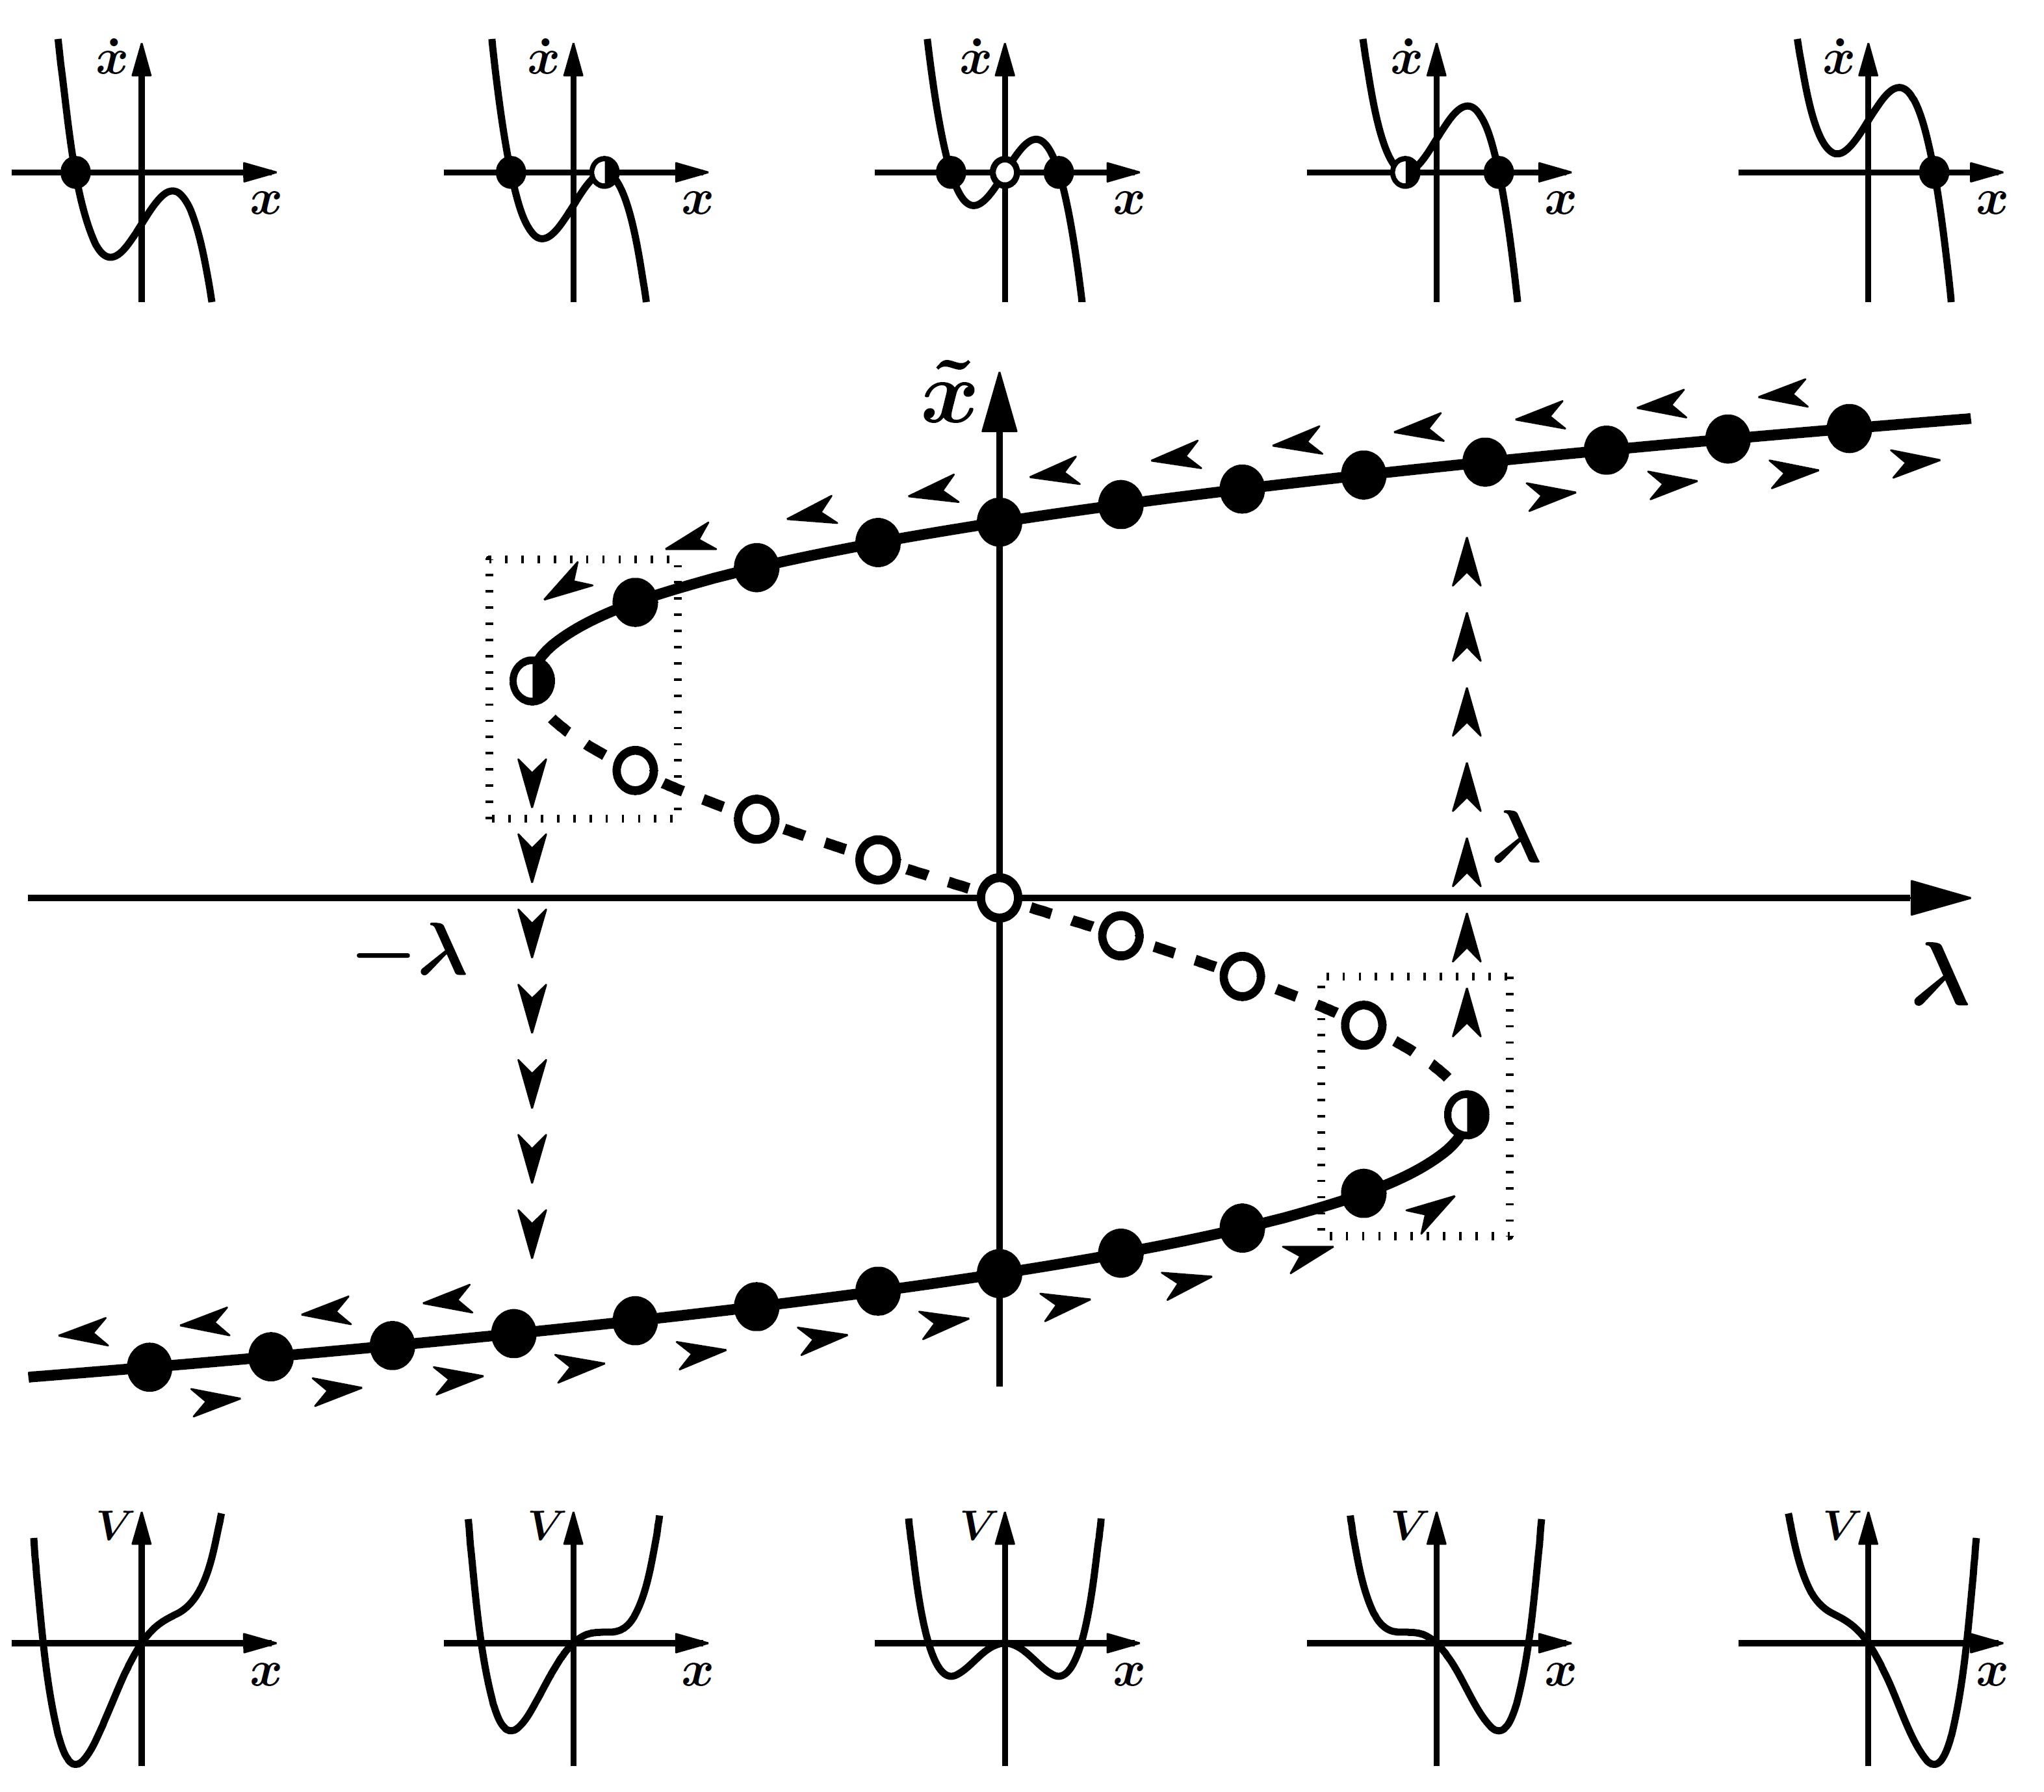
\includegraphics[width=\linewidth]{bfwh1.png}
    \caption{$\dot{x}=\lambda+x-x^3$}
    \label{fig:bfwh1}
  \end{subfigure}
  \vline
  \begin{subfigure}{0.45\linewidth}
    \raggedright
    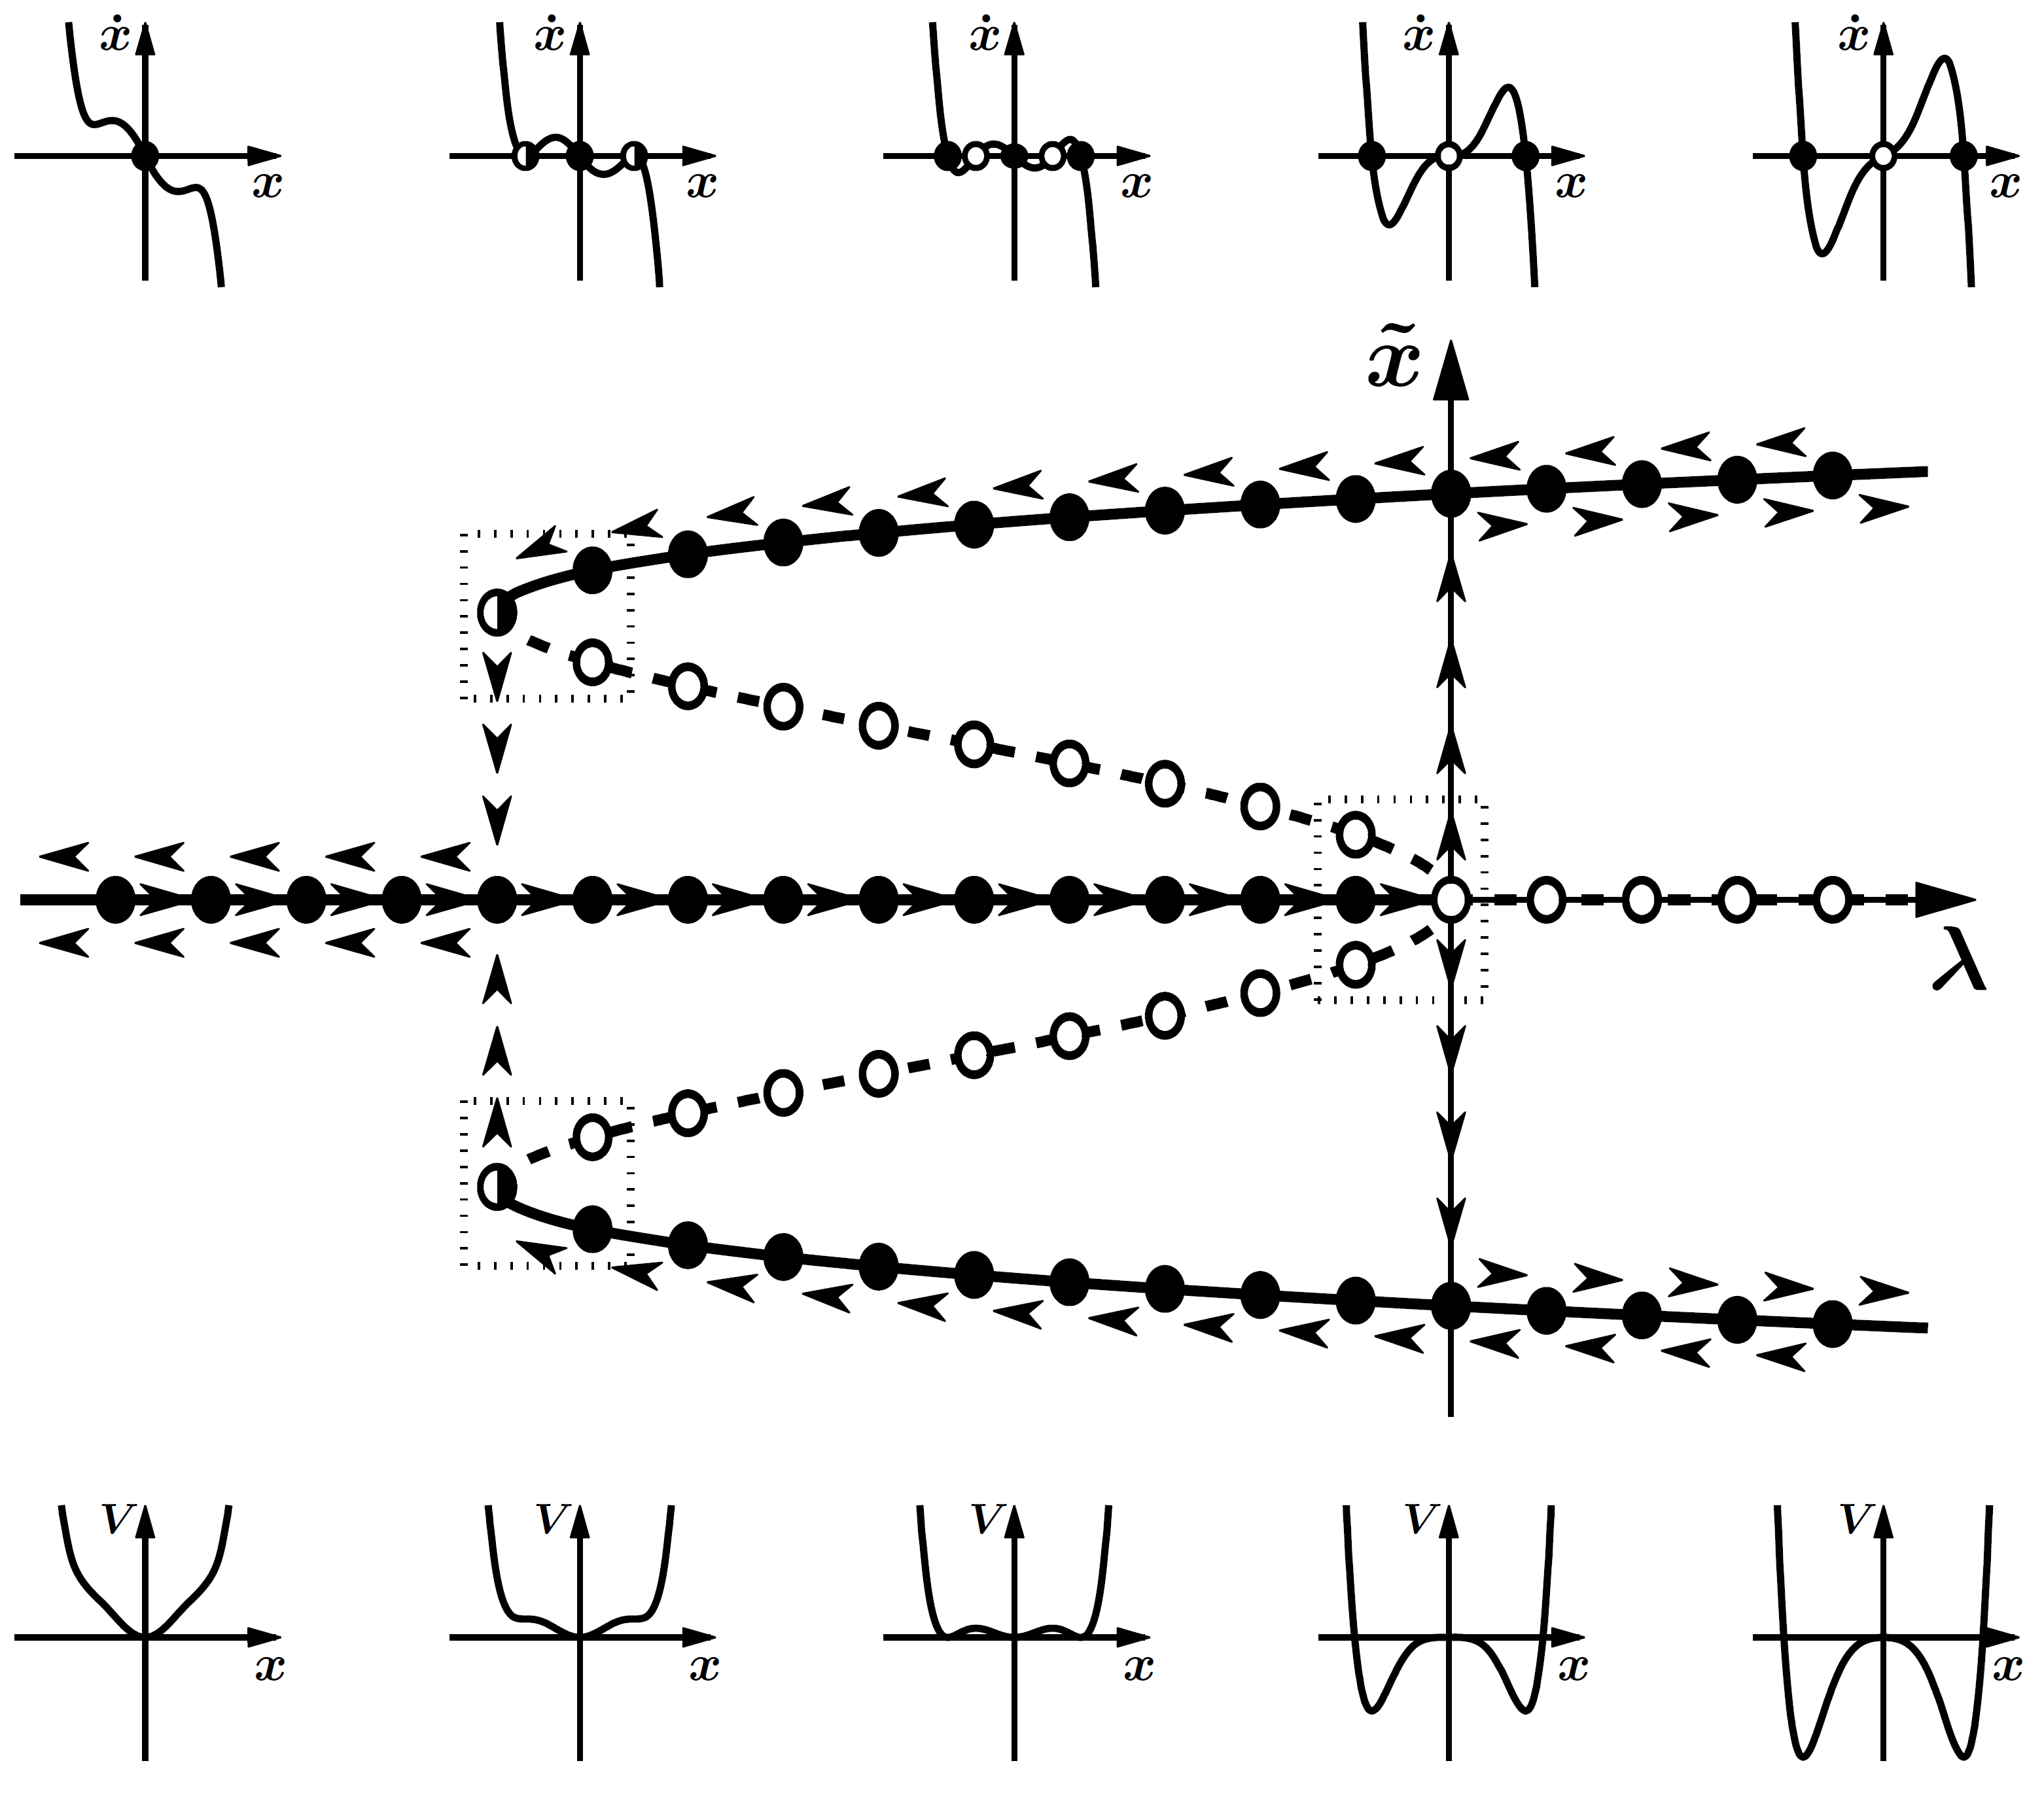
\includegraphics[width=\linewidth]{bfwh2.png}
    \caption{$\dot{x}=\lambda x+x^3-x^5$}
    \label{fig:bfwh2}
  \end{subfigure}
  \caption{Systems showing hysteresis.}
  \label{fig:bfwh}
\end{figure}
\paragraph{Globally Stable Subcritical Pitchfork Bifurcation}
In equation, 
\begin{equation}
\dot{x}=\lambda x+x^3-x^5
\end{equation}
A globally stable version of the subcritical pitchfork bifurcation.
The diagram contains three basic bifurcations indicated by the dotted rectangles in Figure (\ref{fig:bfwh2}).
Beside the subcritical pitchfork bifurcation at the origin there are two saddle-node bifurcations at locations $\lambda=-\frac{1}{4}$, $\tilde{x}=\pm\frac{1}{2}\sqrt{2 }$ in the $\lambda\tilde{x}-$plane.

\newpage
\part{Two Dimensional Systems}
One Dimensional Systems are basically those in equation (\ref{eq:gode}) with $n=2$.
Two-dimensional dynamical systems can be represented by either a single differential equation of second order, which contains a second derivative with respect to time, or by two equations of first order.
In general, a second order system can always be expressed as two first order equations.
\begin{equation}{\label{eq:2d}}
	\begin{aligned}
		\dot{x}&=f(x,y)\\
		\dot{y}&=g(x,y)
	\end{aligned}\quad\text{or}\quad
	\ddot{x}+f(x,\dot{x})=0 \quad \rightarrow \quad 
	\begin{cases} 
		\dot{x}=y&\\
		\dot{y}=-f(x,\dot{x})&
	\end{cases}
\end{equation}
Let's start with

\section{Linear Systems}
A two-dimensional linear system is a system of the form
\begin{equation}
	\begin{aligned}
		\dot{x}=ax+by\\
		\dot{y}=cx+dy
	\end{aligned}
\end{equation}
where $a$, $b$, $c$, $d$ are parameters.
If we use \textbf{boldface} to denote vectors, this system can be written more compactly in matrix form as
\begin{equation}{\label{eq:g2de}}
	\mathbf{\dot{x}}=A\mathbf{x} \quad \text{where} \quad 
	A=
	\begin{pmatrix}
		a&b\\c&d
	\end{pmatrix}\quad\text{and}\quad
	\mathbf{x}=
	\begin{pmatrix}
		x\\y
	\end{pmatrix}\quad
	\mathbf{\tilde{x}}=
	\begin{pmatrix}
		0\\0
	\end{pmatrix}
\end{equation} 
Notice that $\mathbf{\dot{x}}=0$ when $\mathbf{x}=0$, so $\mathbf{\tilde{x}}$ is always a fixed point for any choice of $A$.
The solutions of $\mathbf{\dot{x}}=A\mathbf{x}$ can be visualized as trajectories moving on the $(x,y)$ plane, in this context called the {\textbf{phase plane}}.\\\\
If the off-diagonal terms in (\ref{eq:g2de}), $b$ and $c$ are zero, we would have two seperate uncoupled equations in $x$ and $y$ (Equation (\ref{eq:c2de})).
Such kind of systems are called \textbf{Uncoupled Systems}.
However, there would be two special lines, where the trajectories starting on it would always stick to it, these are  $x$ and $y$ axes\label{txt:xya}.\\
Suppose $d=-1$, then the system has solution as shown in Figure (\ref{fig:cnls}).
\begin{equation}{\label{eq:c2de}}
	\begin{aligned}
		\dot{x}=ax\\
		\dot{y}=dy
	\end{aligned}\quad\rightarrow\quad
	\begin{aligned}
		A=\begin{pmatrix}
		a&0\\0&d
		\end{pmatrix}
	\end{aligned}\quad\rightarrow\quad
	\begin{aligned} 
		x(t)=x_0e^{at}\\
		y(t)=y_0e^{dt}
	\end{aligned}
\end{equation}
\begin{figure}[h!]
	\centering
	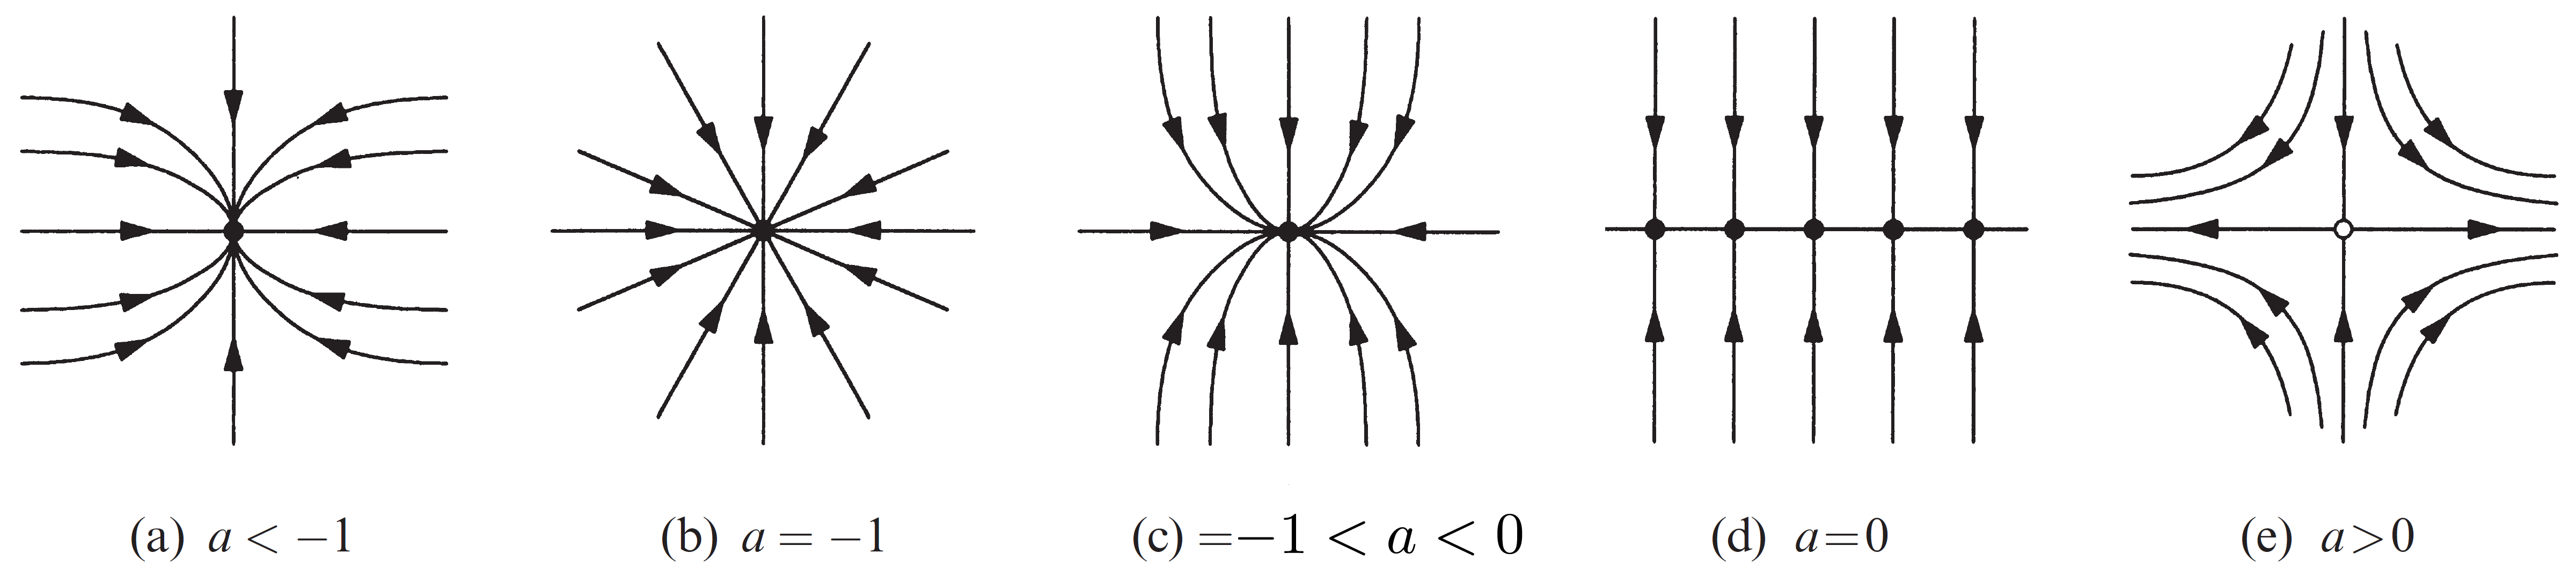
\includegraphics[width=0.9\linewidth]{cnls.png}
	\caption{Phase Portrait of Equation (\ref{eq:c2de}). See Section (\ref{sec:cls}) for classification.}
	\label{fig:cnls}
\end{figure}
\subsection{Classification of Two-Dimensional Linear Systems}{\label{sec:cls}}
There is the possibility of special lines (like $x$ and $y$ axis in case of uncoupled systems) existing for a general linear system having a matrix $A$.
The equation for finding such a direction is
\begin{equation}
	A\mathbf{x}=\lambda\mathbf{x}
\end{equation}
This is precisely the form of the eigenvalue problem whose solution is well known in the domain of linear algebra.
The eigenvalues of $A$ can be readily calculated and it is most convenient to express them in terms of the trace $(t_r)$ and determinant $(d_{et})$ of $A$.
\begin{equation}
	\begin{vmatrix}
		a-\lambda&b\\c&d-\lambda
	\end{vmatrix}
	=\lambda^2-\lambda\underbrace{(a+d)}_{t_r}+\underbrace{ad-bc}_{d_{et}}=0
\end{equation}
\begin{equation}
	\Rightarrow \lambda_{1,2}=\frac{1}{2}\{t_r\pm\sqrt{t_r^2-4d_{et}}\}
\end{equation}
The trace and determinant are invariant when the matrix $A$ is expressed by its eigenvalues and becomes diagonal
\begin{equation}
	A=
	\begin{pmatrix}
		\lambda_1&0\\0&\lambda_2
	\end{pmatrix}
	\quad \text{as} \quad
	\begin{aligned}
		\lambda_1+\lambda_2&=t_r\\
		\lambda_1\lambda_2&=d_{et}
	\end{aligned}
\end{equation}
\begin{enumerate}[label=\textbf{(\Alph*)}]
	\item Eigenvalues are Real
		\begin{equation}
			t_r^2-4d_{et}\geq0 \quad\rightarrow\quad \lambda_{1,2}\in\mathbb{R}
		\end{equation}
		\begin{enumerate}
			\item[\textbf{Case: (1.a)}]  $\lambda_1<\lambda_2<0$\quad|\quad\fbox{
	  			\mbox{$t_r^2-4d_{et}>0\quad d_{et}>0\quad t_r<0$}}\\
				This case is called a {\textbf{stable node}}, the only straight trajectories are along the eigendirections, which are given by the eigenvectors of the system.
				As $\lambda_1<\lambda_2$, the trajectories approach the fixed point faster along the direction of the eigenvector $\mathbf{v^{(1)}}$ which corresponds to $\lambda_1$, and is therefore called the \emph{fast eigendirection}.
				In the same way, the direction related to $\lambda_2$ is called the \emph{slow eigendirection}.
				\begin{figure}[h!]
					\centering
					\begin{subfigure}{0.4\linewidth}
						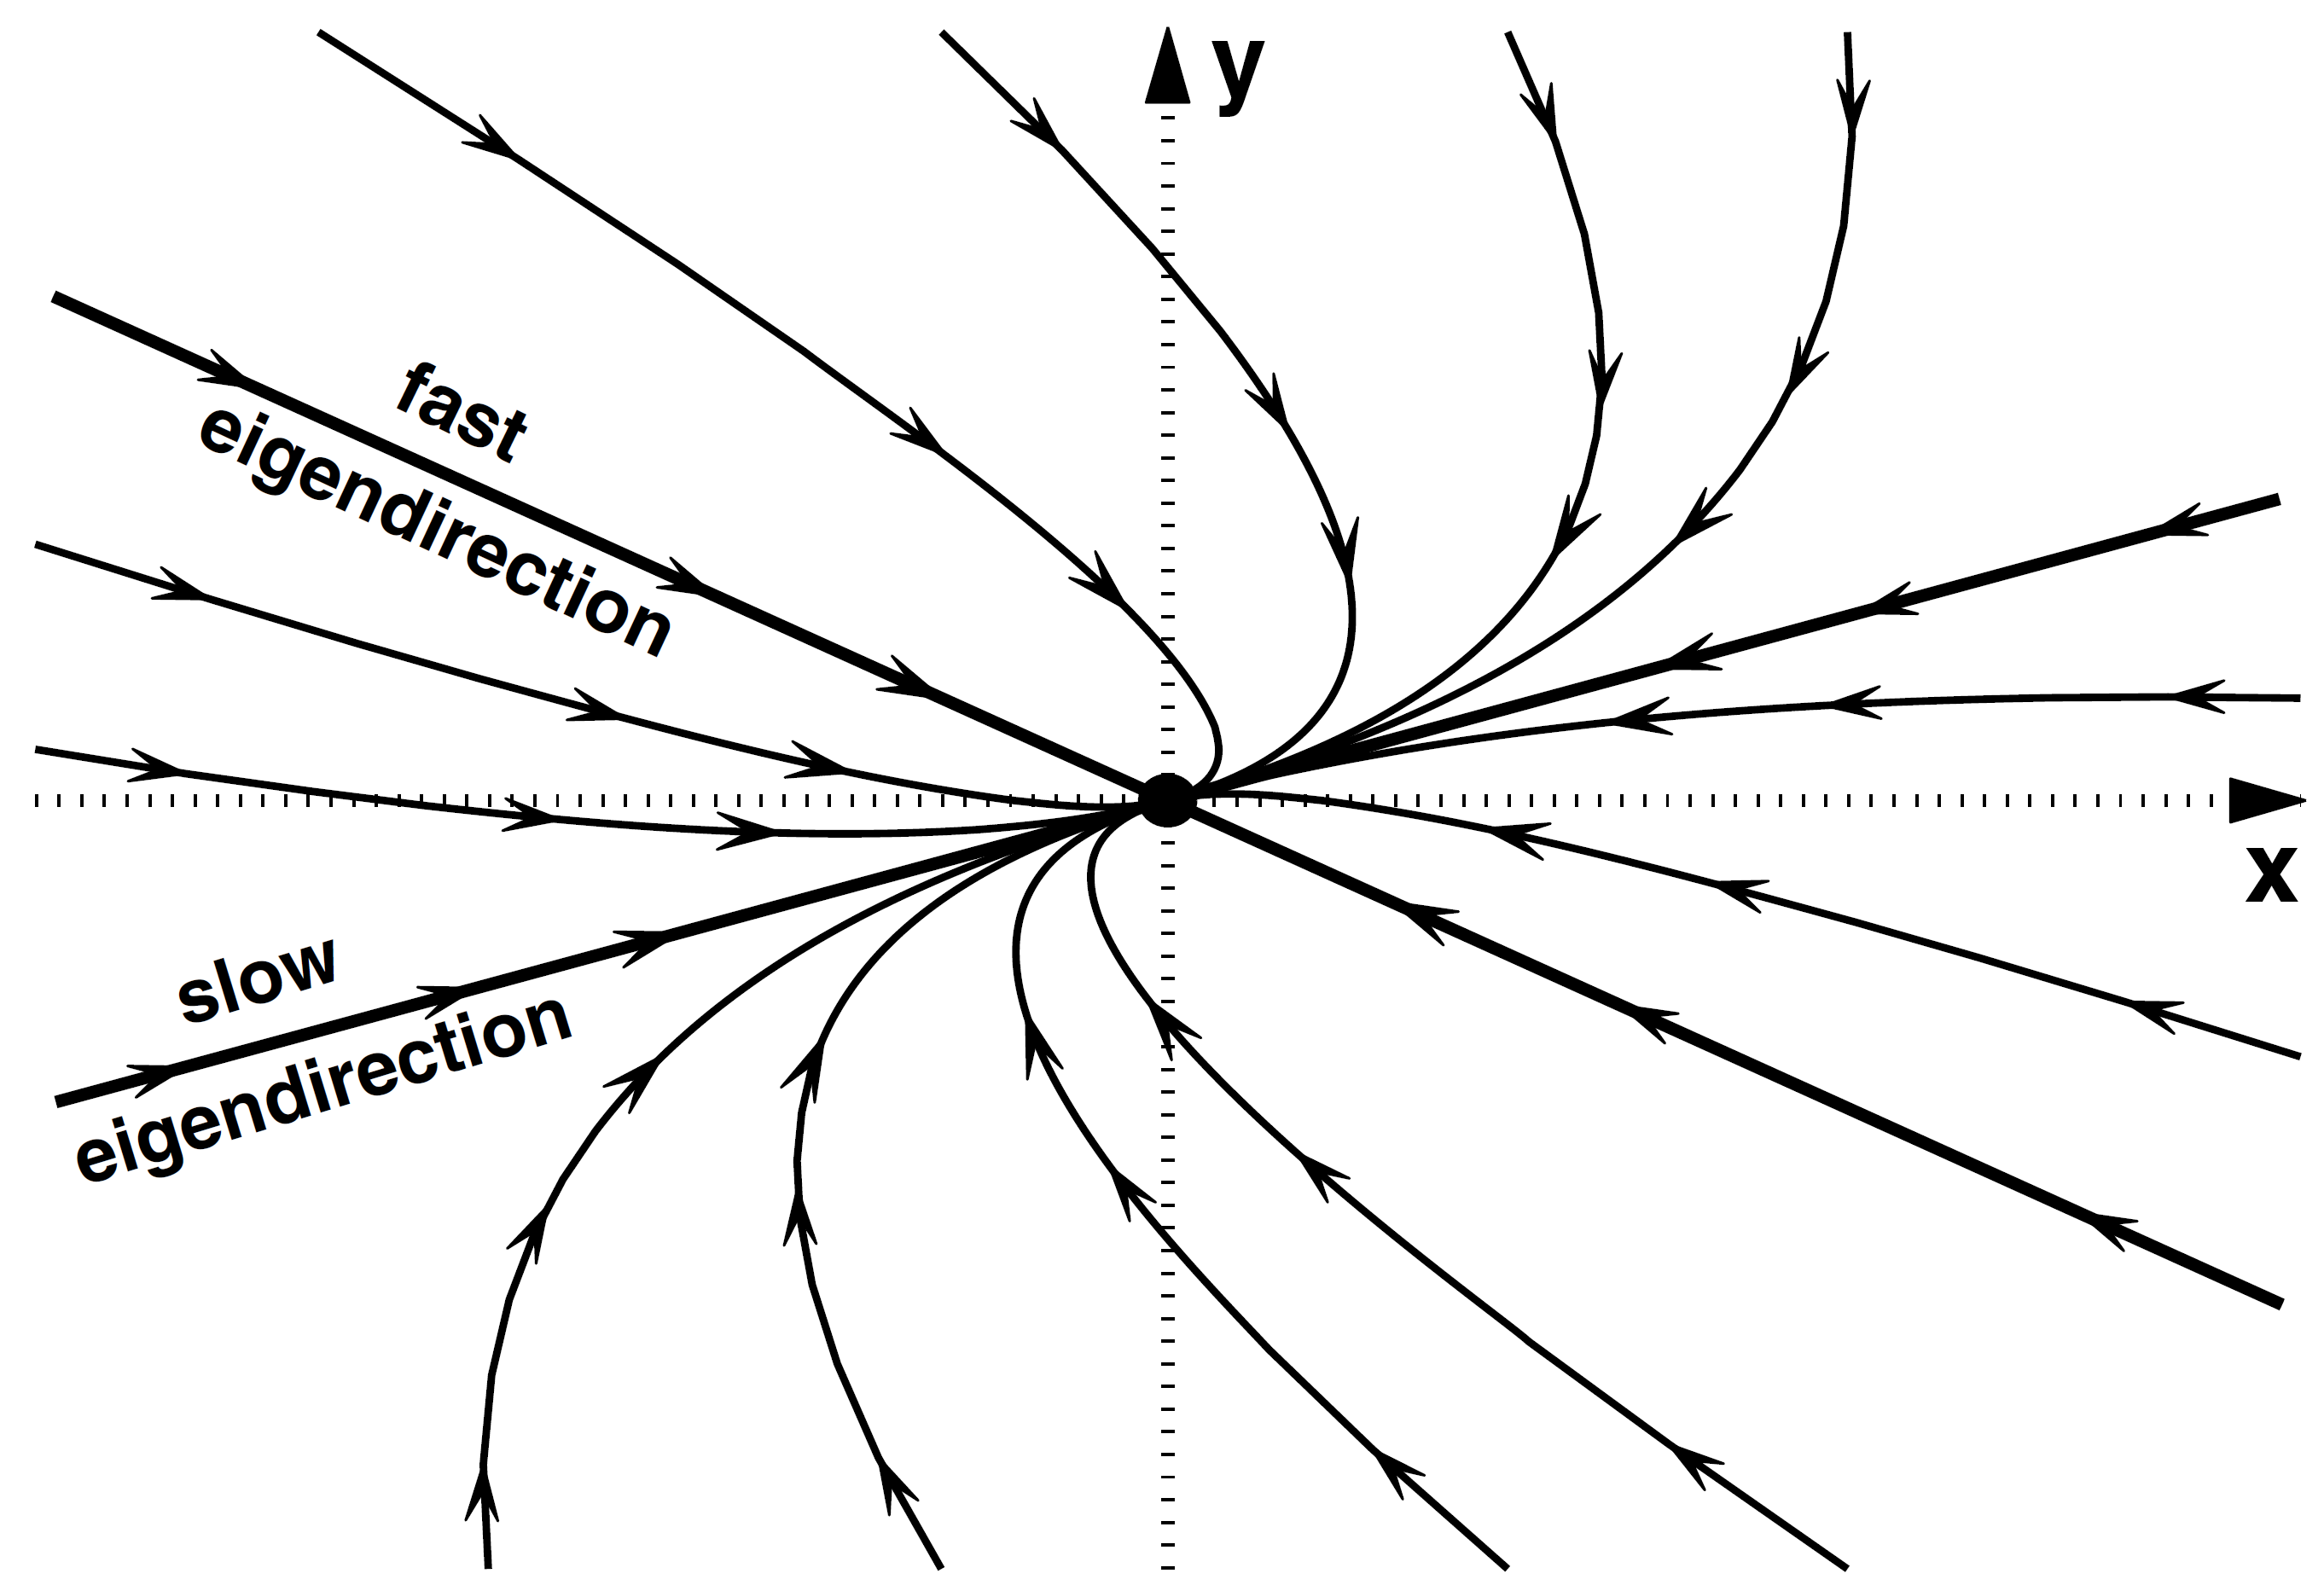
\includegraphics[width=\linewidth]{snls.png}
						\caption{Phase Portrait of a Stable Node}
						\label{fig:snls}
					\end{subfigure}
					\vline
					\begin{subfigure}{0.364\linewidth}
						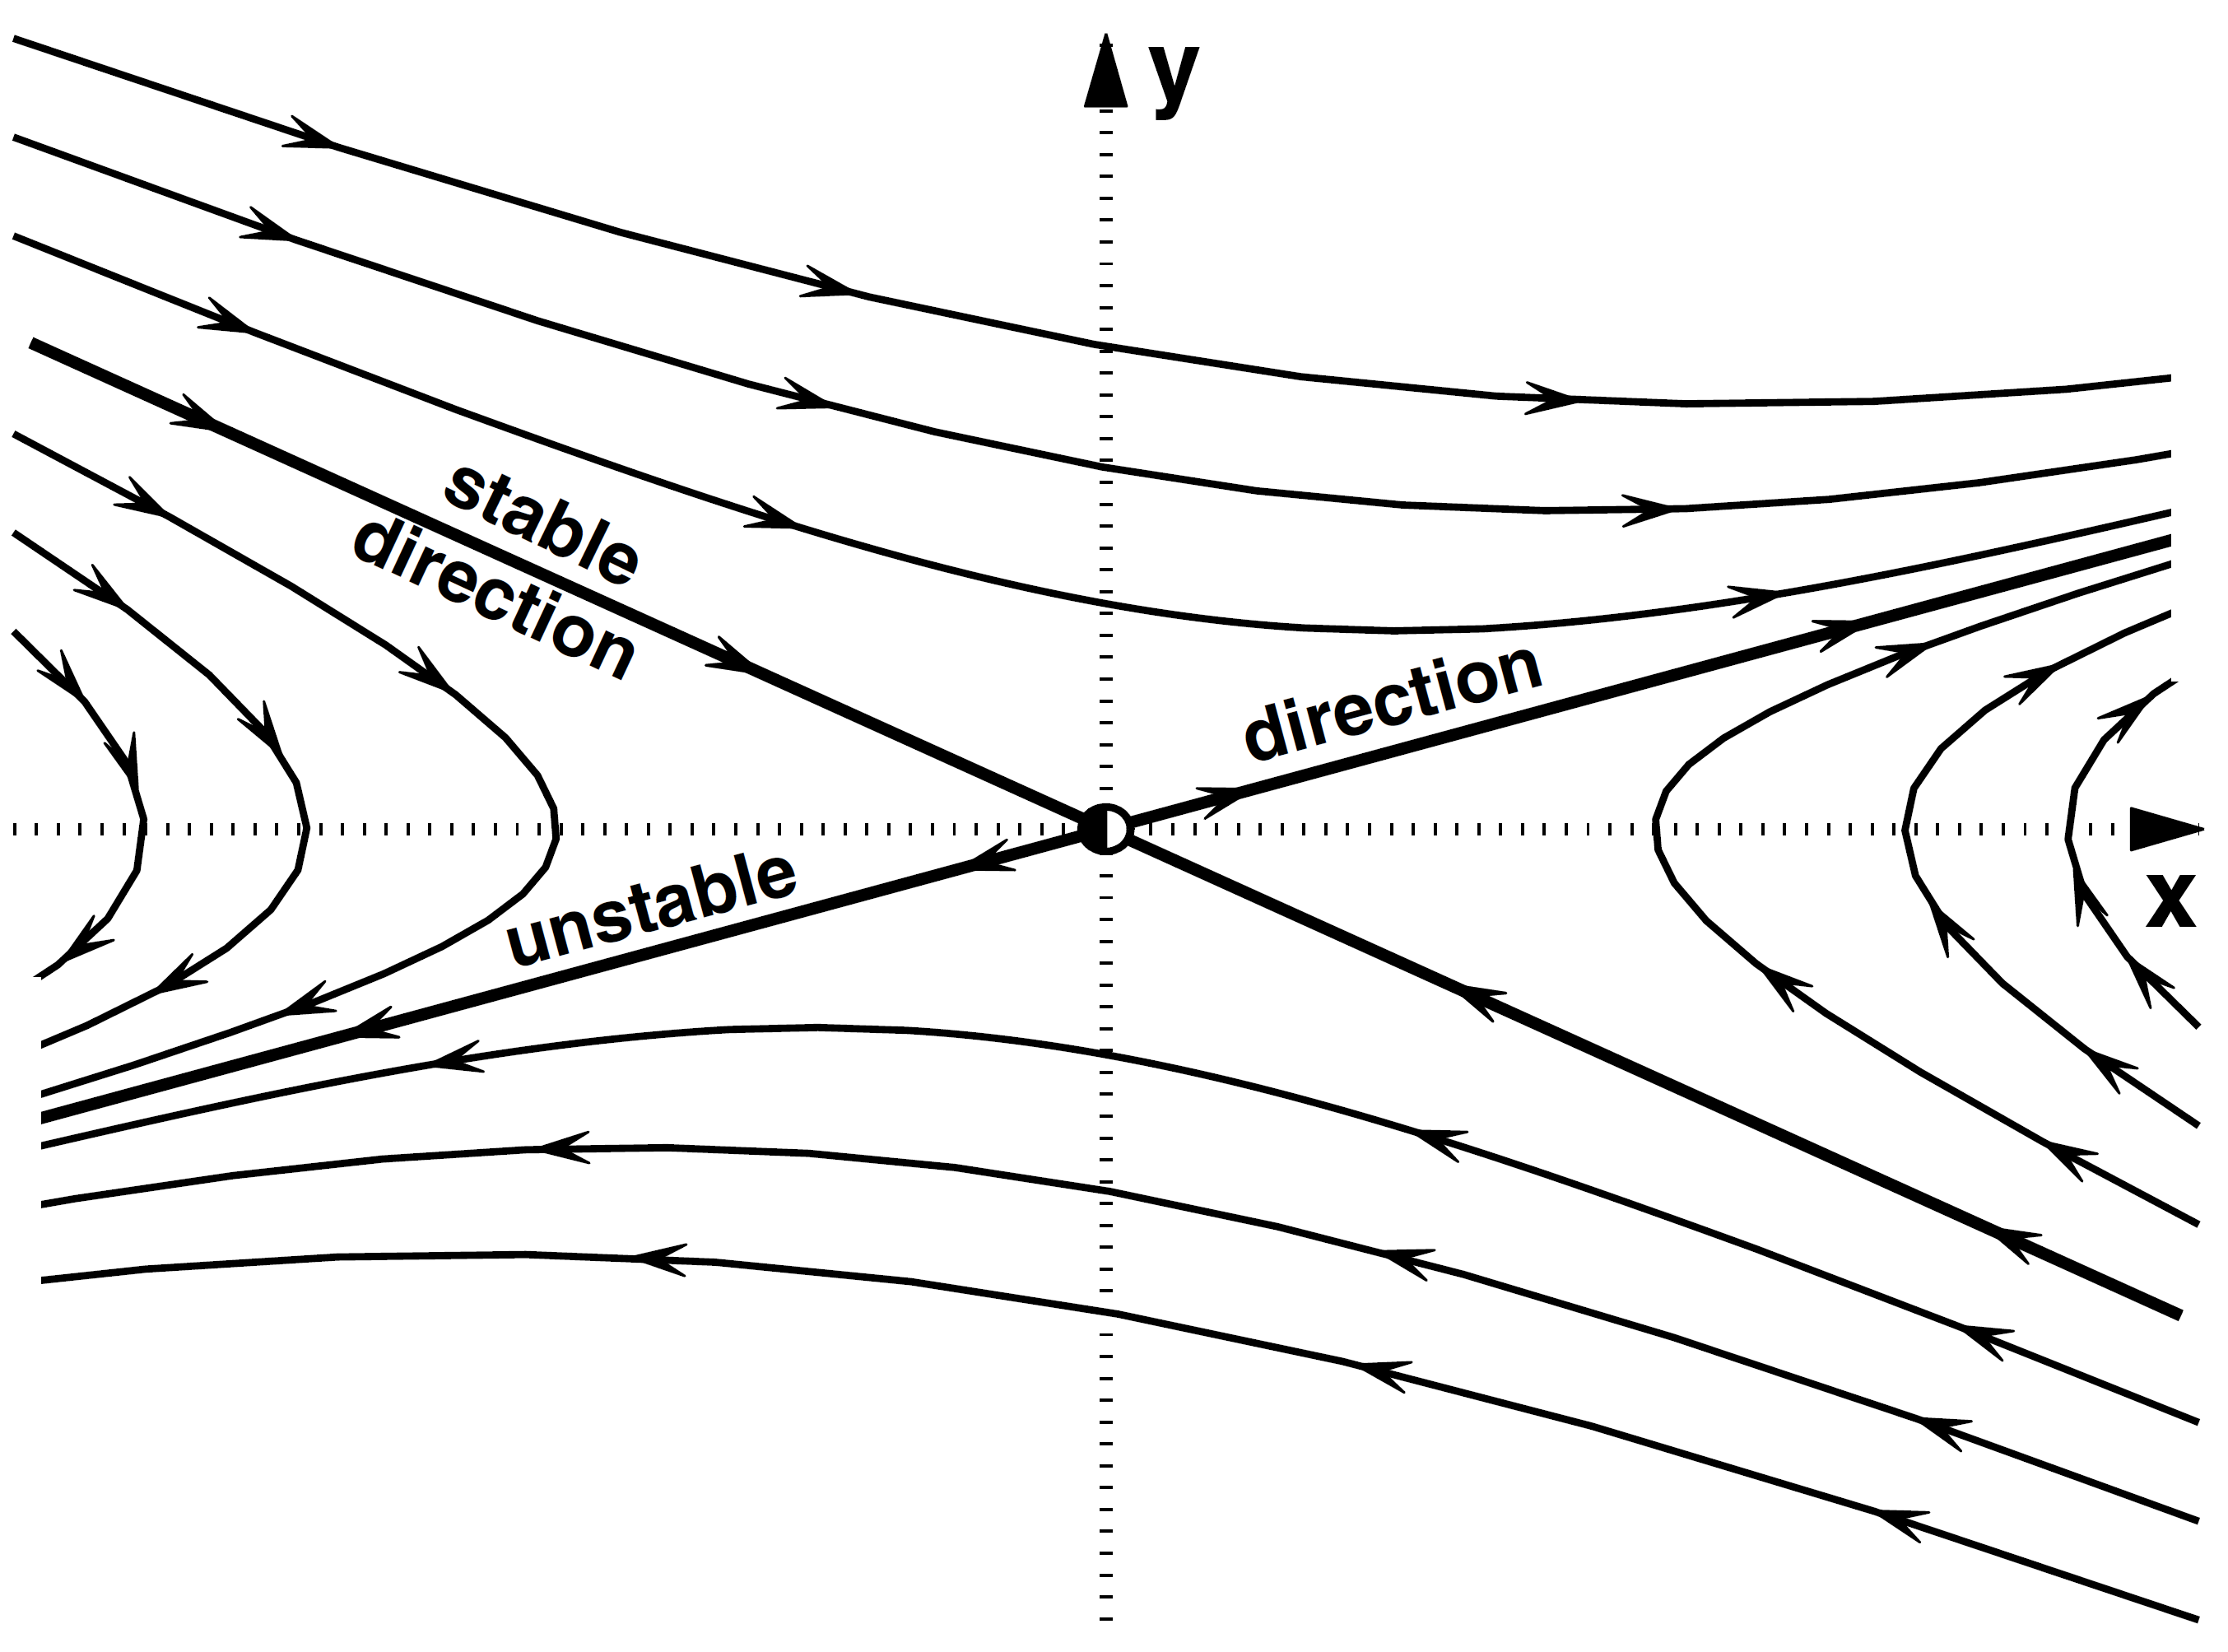
\includegraphics[width=\linewidth]{spls.png}
						\caption{Phase Portrait of a Saddle Point}
						\label{fig:spls}
					\end{subfigure}
					\caption{}
					\label{fig:cls1}
		    	\end{figure}
		    \item[\textbf{Case: (1.b)}] $0<\lambda_2<\lambda_1$\quad|\quad \fbox{
	  			\mbox{$t_r^2-4d_{et}>0\quad d_{et}>0\quad t_r>0$}}\\
		    	Correspondingly, for the phase space plot when both eigenvalues are positive, the flow, indicated by the arrows in Figure (\ref{fig:cls1}), is reversed and leads away from the fixed point, which is then called an {\textbf{unstable node}}.	    
		    \item[\textbf{Case: (2)}] $\lambda_1<0<\lambda_2$\quad|\quad \fbox{
	  			\mbox{$t_r^2-4d_{et}>0\quad d_{et}<0$}}\\
		    	If one of the eigenvalues is positive and the other negative, the fixed point at the origin is \emph{half-stable} and called a {\textbf{saddle point}}.
		    	The eigenvector that corresponds to the negative eigenvalue defines the direction where the flow in phase space is pointing towards the fixed point, the so-called {\textbf{stable manifold}} (stable direction), defined as the set of initial conditions $\mathbf{x}_0$ such that $\mathbf{x}(t)\rightarrow\mathbf{\tilde{x}}$ as $t\rightarrow\infty$.
		    	The positive eigenvalue is associated with the {\textbf{unstable manifold}} (unstable direction) which is set of initial conditions $\mathbf{x}_0$ such that $\mathbf{x}(t)\rightarrow\mathbf{\tilde{x}}$ as $t\rightarrow-\infty$.
		    	Here, the flow moves away from the fixed point\footnote{Note that a typical trajectory asymptotically approaches the unstable manifold as $t\rightarrow\infty$, and approaches the stable manifold as $t\rightarrow-\infty$.}. A typical phase space portrait is shown in Figure (\ref{fig:spls}).\\ \\	
		    	Now, let's see \emph{degenerate} cases
		    \item[\textbf{Case: (3.a)}] $\lambda_1=\lambda_2<0$\quad|\quad \fbox{
	  			\mbox{$t_r^2-4d_{et}=0\quad d_{et}>0\quad t_r<0$}}\\
		    	Let look at the system with
		    	\begin{equation}
			    	A=
			    	\begin{pmatrix}
				    	\lambda&b\\0&\lambda
			    	\end{pmatrix}\quad\rightarrow\quad \lambda_{1,2}=\lambda
		    	\end{equation}
		    	Then Eigenvectors are given by
		    	\begin{equation}
			    	\begin{pmatrix}
				    	\lambda&b\\0&\lambda
			    	\end{pmatrix}
			    	\begin{pmatrix}
				    	v_x\\v_y
			    	\end{pmatrix}=
			    	\lambda
			    	\begin{pmatrix}
				    	v_x\\v_y
			    	\end{pmatrix}
			    	\quad\rightarrow\quad
			    	\begin{aligned}
				    	\lambda v_x+bv_y&=\lambda v_x\\\lambda v_y&=\lambda v_y
			    	\end{aligned}
			    	\quad\rightarrow\quad
			    	bv_y=0
		    	\end{equation}
		    	\begin{enumerate}[label=(\roman*)]
			    	\item $b\neq0$\\
			    	The only eigendirection of $A$ is the horizontal axis with $v_y=0$. The fixed point is called a \emph{stable} {\textbf{degenerate node}} and its phase portrait shown in Figure (\ref{fig:stnls} left).
			    	\item $b=0$\\
			    	Any vector is an eigenvector and the trajectories are straight lines pointing towards the fixed point. The phase space portrait for this situation is shown in Figure (\ref{fig:stnls} right) and the fixed point is for obvious reasons called a \emph{stable} {\textbf{star node}}.
		    	\end{enumerate}
		    	\begin{figure}[h!]
					\centering
					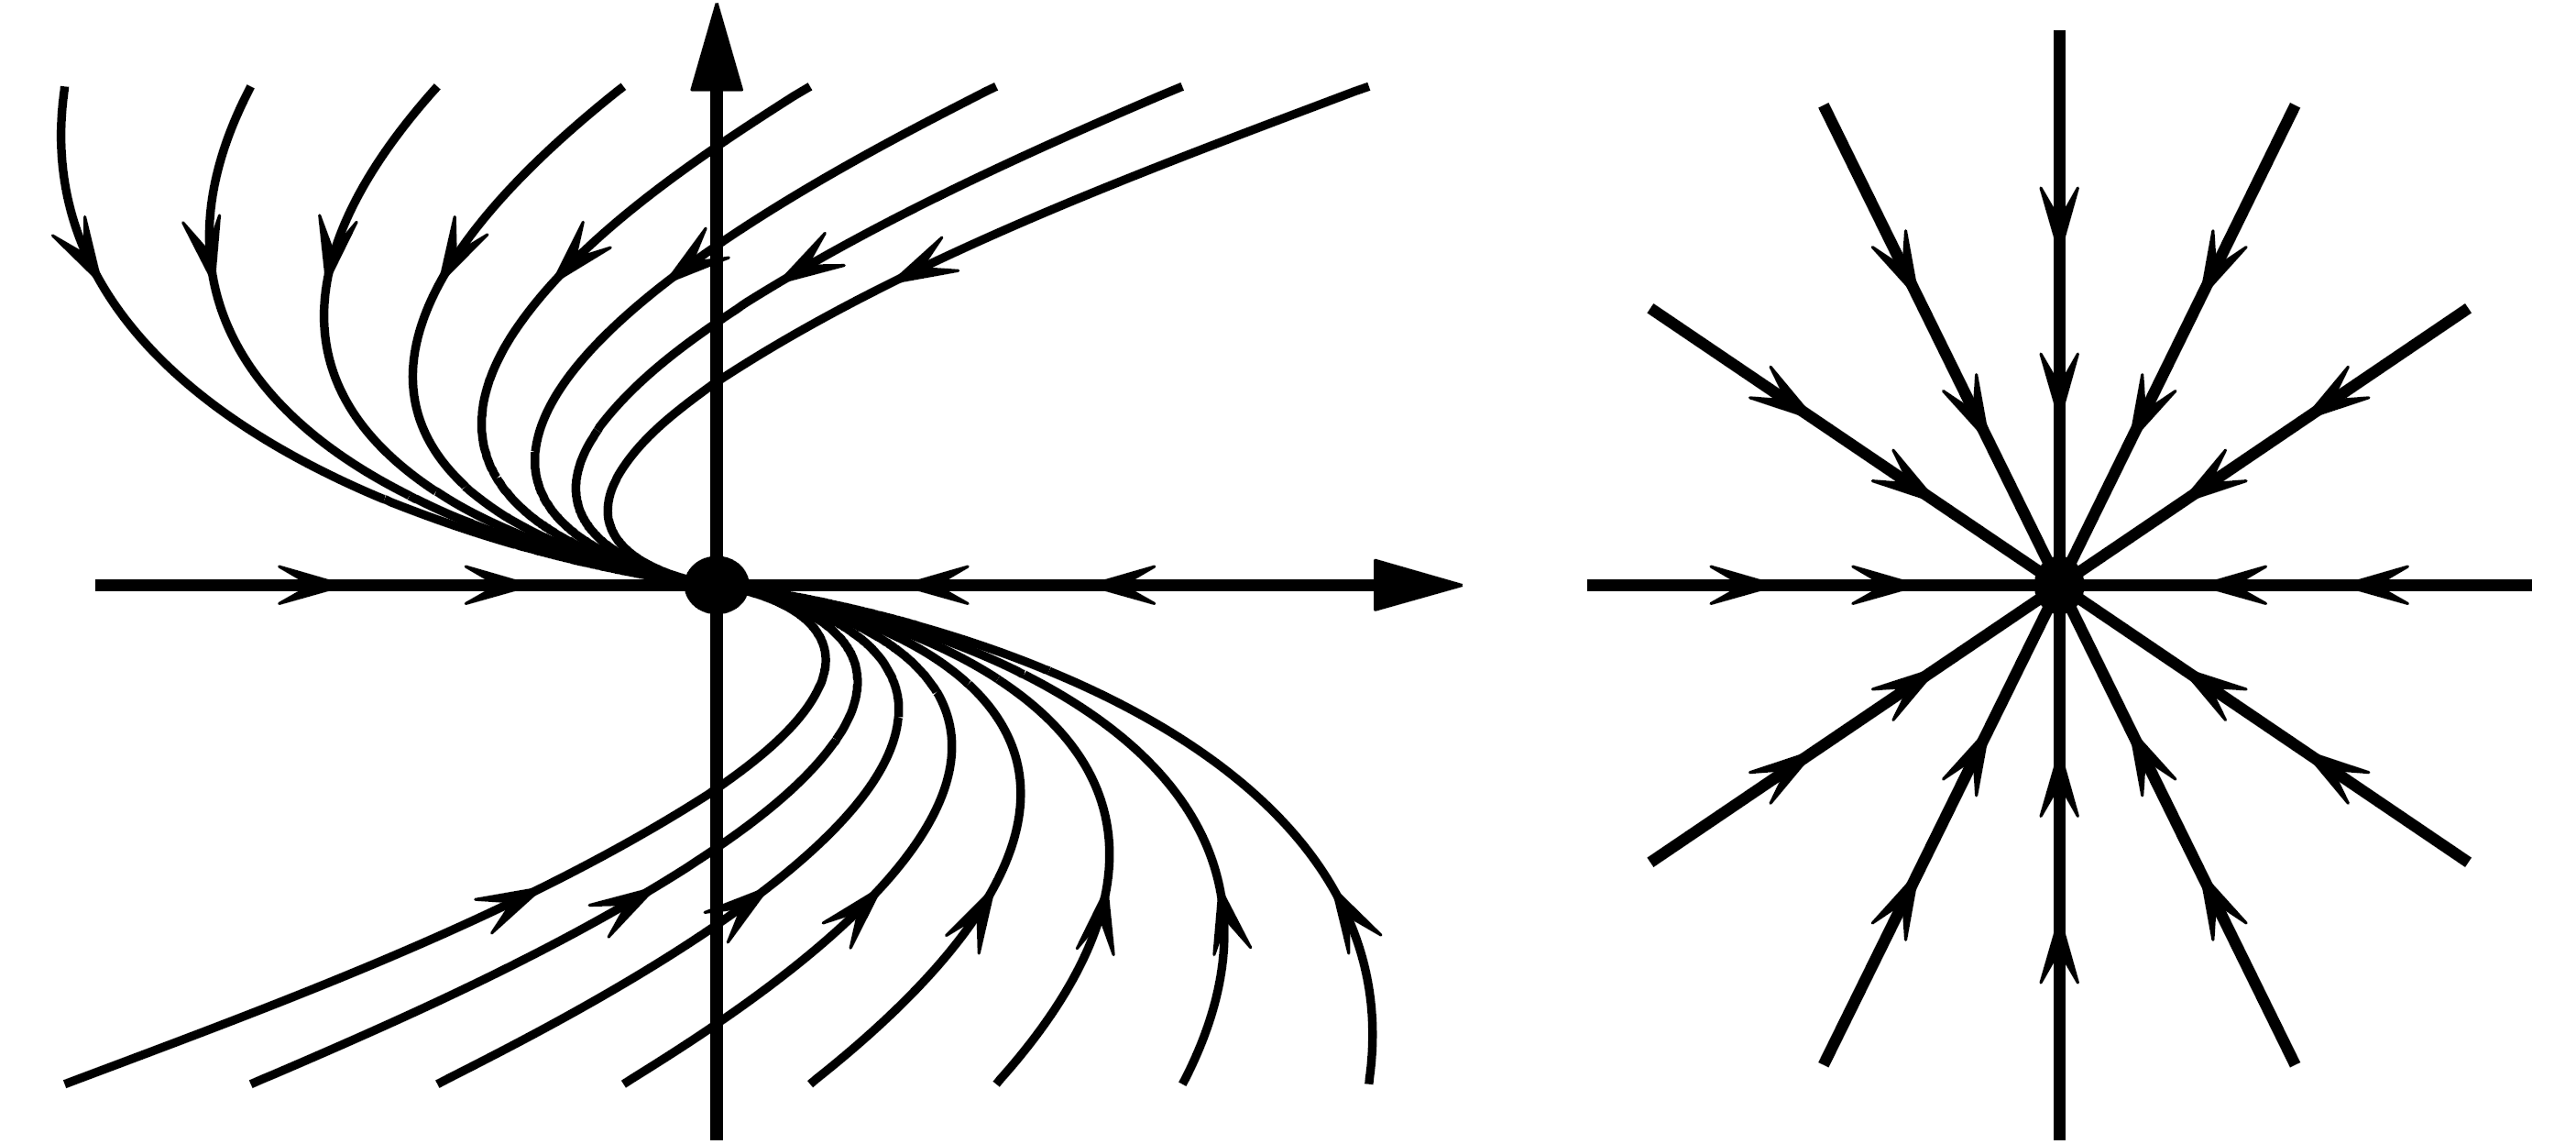
\includegraphics[width=0.6\linewidth]{dnls.png}
					\caption{Degenerate case where the eigenvalues are the same. The degenerate node (left) has only one eigendirection, the star node (right) has infinitely many.}
					\label{fig:stnls}
		    	\end{figure}
		    \item[\textbf{Case: (3.b)}] $\lambda_1=\lambda_2>0$\quad|\quad \fbox{
	  			\mbox{$t_r^2-4d_{et}=0\quad d_{et}>0\quad t_r>0$}}\\
		    	Similar as above
				\begin{enumerate}[label=(\roman*)]
			    	\item $b\neq0$\\
			    	The only eigendirection of $A$ is the horizontal axis with $v_y=0$.The flow, indicated by the arrows in Figure (\ref{fig:stnls} left), is reversed and leads away from the fixed point which is called a \emph{unstable} {\textbf{degenerate node}}.
			    	\item $b=0$\\
			    	Any vector is an eigenvector and the trajectories are straight lines pointing away from the fixed point.
			    	The flow, indicated by the arrows in Figure (\ref{fig:stnls} left), is reversed and the fixed point is for obvious reasons called a \emph{unstable} {\textbf{star node}}.
		    	\end{enumerate}	    
		    \item[\textbf{Case: (4.a)}] $\lambda_1<\lambda_2=0$\quad|\quad \fbox{
	  			\mbox{$t_r^2-4d_{et}>0\quad d_{et}=0\quad t_r<0$}}\\	
		    	Here, tragectories are parallel and towards a line of fixed points.
		    	The fixed point is {\textbf{Lyapunov stable}}\footnote{It means if all trajectories that start sufficiently close to $\mathbf{x}$ remain close to it for all time.} (Figure (\ref{fig:snils}) left).
		    \item[\textbf{Case: (4.b)}] $0=\lambda_1<\lambda_2$\quad|\quad \fbox{
	  			\mbox{$t_r^2-4d_{et}>0\quad d_{et}=0\quad t_r>0$}}\\
		    	Here, tragectories are parallel and towards a line of fixed points.
		    	These are \emph{unstable} {\textbf{non-isolated}} (Figure (\ref{fig:snils}) right).
				\begin{figure}[h!]
					\centering
					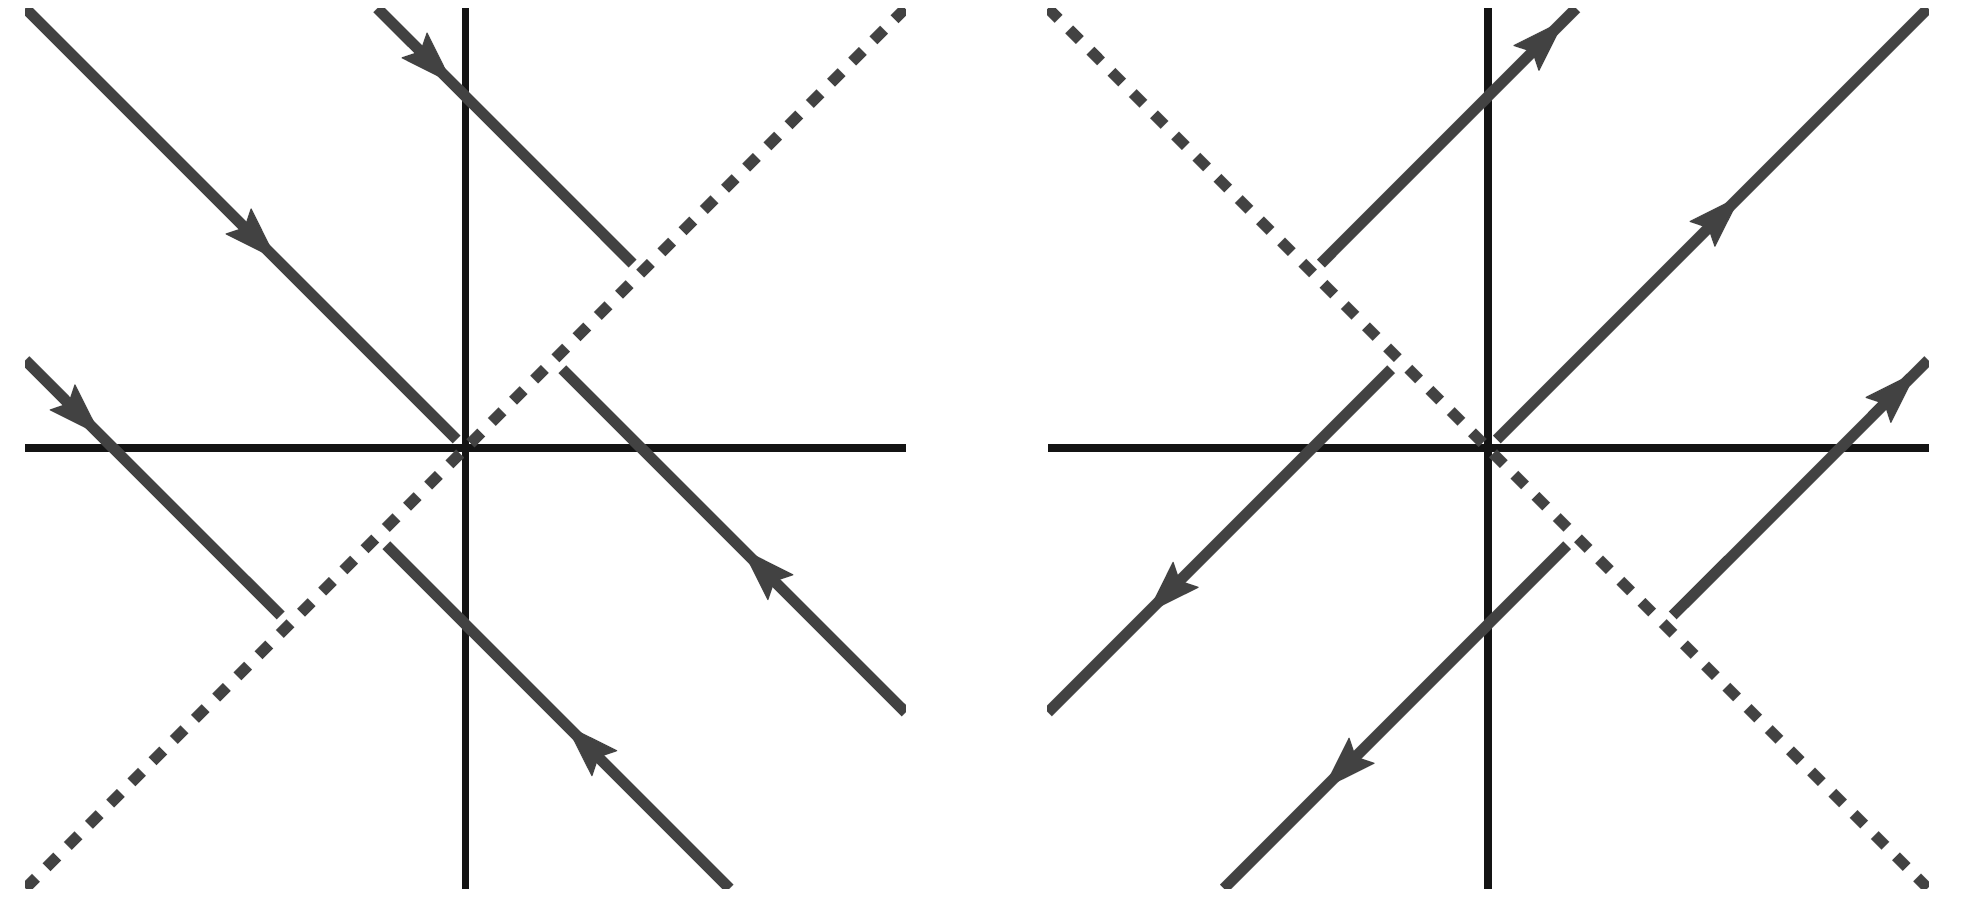
\includegraphics[width=0.4\linewidth]{snils.png}
					\caption{\emph{Stable non-isolated} fixed points on left and \emph{unstable non-isolated} fixed points on right }
					\label{fig:snils}
		    	\end{figure}
	    	\item[\textbf{Case: (5)}] $\lambda_1=\lambda_2=0$\quad|\quad \fbox{
	  			\mbox{$t_r^2-4d_{et}=0\quad d_{et}=0\quad t_r=0$}}\\
	    	Non-isolated fixed point, a plane of fixed points.
	    	Nothing happens and nothing can happen! Remember (\ref{eq:cons})?
		\end{enumerate}
	\item Eigenvalues are Complex (In fact, they are Complex Conjugate)
		\begin{equation}
			t_r^2-4d_{et}<0 \quad\rightarrow\quad \lambda_{1,2}\in\mathbb{C} \quad\rightarrow\quad \lambda_2=\lambda_1^\ast, \quad\text{Let} \ \Re(\lambda_{1,2})=\lambda\ \text{and}\ \Im(\lambda_{1,2})\neq0
		\end{equation}
		\begin{itemize}
			\item $\lambda<0$\quad|\quad \fbox{
	  		\mbox{$t_r^2-4d_{et}<0\quad d_{et}>0\quad t_r<0$}}\\
			The trajectories in phase space are spiraling towards from the origin as a {\textbf{stable spiral}} (Figure (\ref{fig:ccels}) left).
			\item $\lambda>0$\quad|\quad \fbox{
	  		\mbox{$t_r^2-4d_{et}<0\quad d_{et}>0\quad t_r>0$}}\\
			The trajectories in phase space are spiraling away from the origin as a {\textbf{unstable spiral}} (Figure (\ref{fig:ccels}) middle).
			\item $\lambda=0$\quad|\quad \fbox{
	  		\mbox{$t_r^2-4d_{et}<0\quad d_{et}>0\quad t_r=0$}}\\
			The trajectories are closed orbits.
			The fixed point $\tilde{x}=0$ is {\textbf{Lyapunov stable}}.
			The fixed point at the origin is neutrally stable and called a {\textbf{center}} (Figure (\ref{fig:ccels}) right).
			\begin{figure}[H]
				\centering
				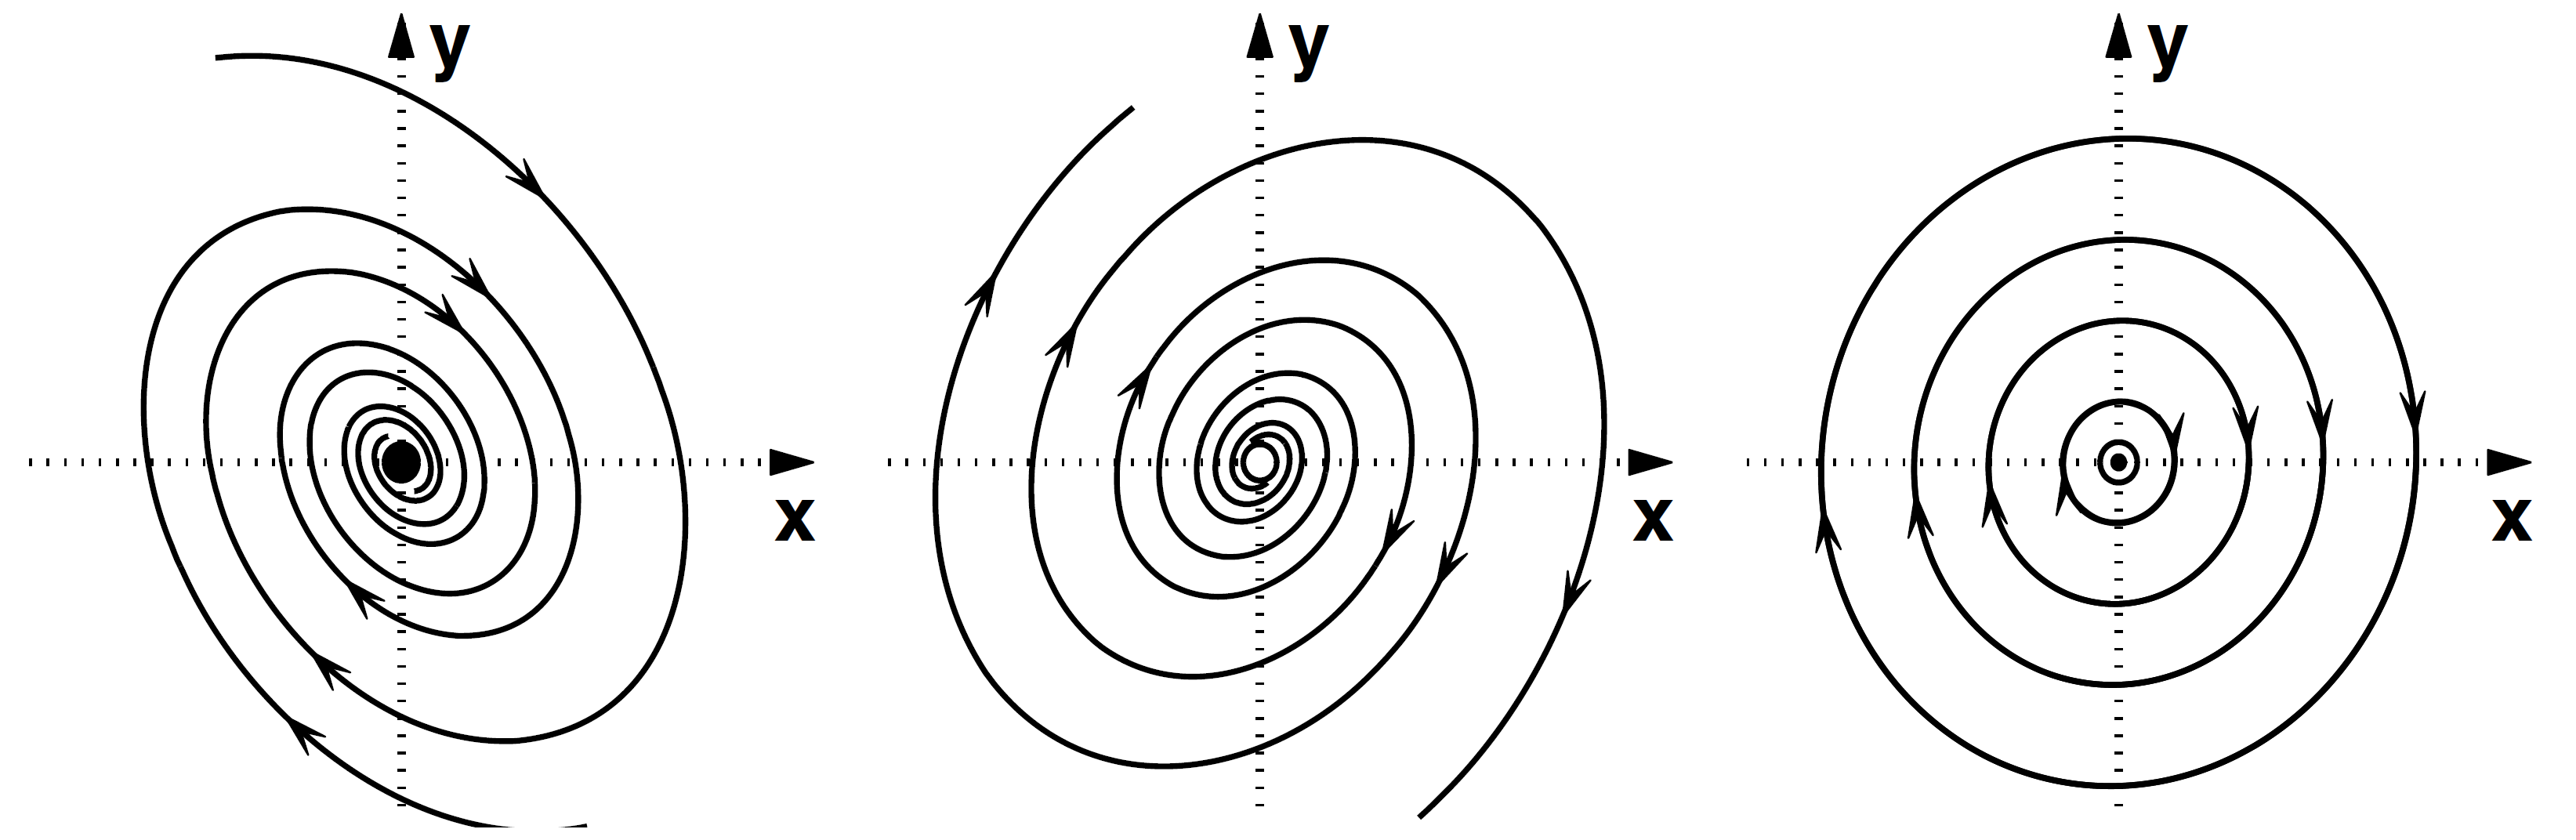
\includegraphics[width=0.5\linewidth]{ccels.png}
				\caption{For complex eigenvalues the trajectories in phase space are stable spirals if their real part is negative (left) and unstable spirals for a positive real part (middle). If the real part of the eigenvalues vanishes the trajectories are closed orbits around the origin, which is then a neutrally stable fixed point called a center (right).}
				\label{fig:ccels}
		    \end{figure}	
		\end{itemize}		
\end{enumerate}
\subsubsection{Summary}
On the left of the vertical axis $(d_{et}<0)$ are the saddle points.
On the right $(d_{et}>0)$ are the centers on the horizontal axis $(t_r=0)$ with unstable and stable spirals located above and below, respectively.
The stars and degenerate nodes exist along the parabola $t_r^2=4d_{et}$ that separates the spirals from the stable and unstable nodes.
\begin{figure}[h!]
	\centering
	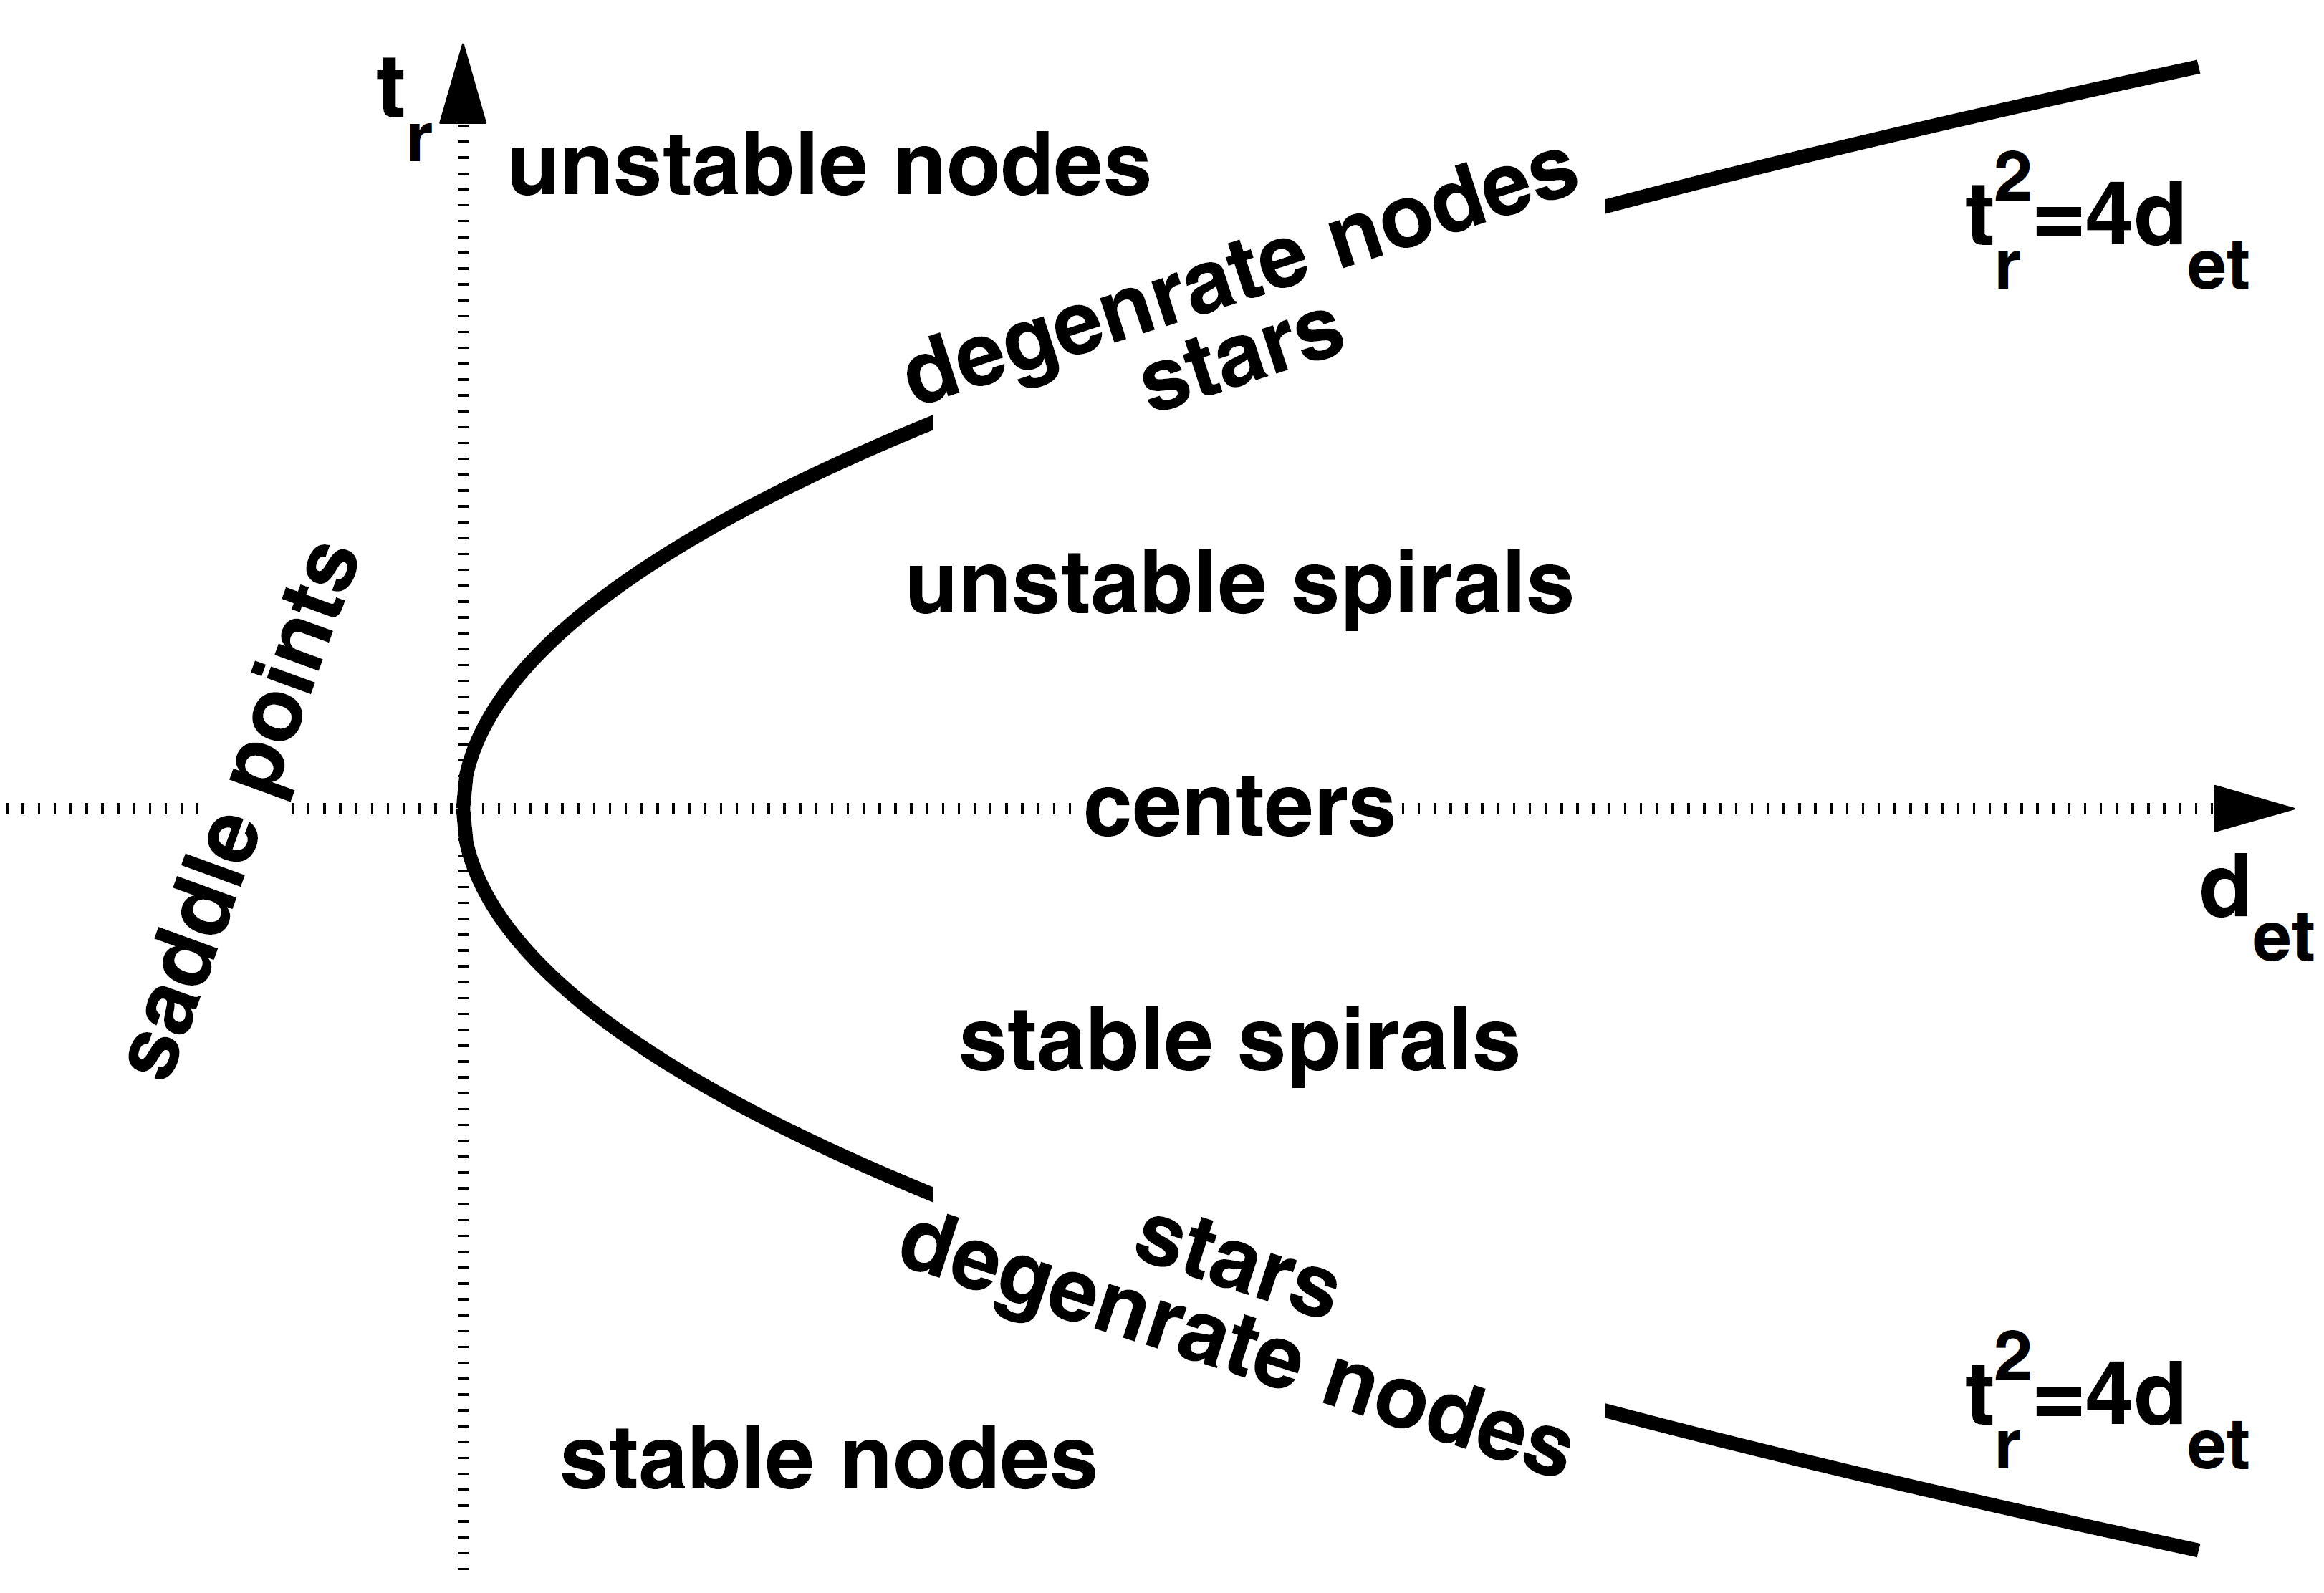
\includegraphics[width=0.5\linewidth]{sumls.png}
	\caption{Classification diagram for two-dimensional linear systems in terms of the trace $t_r$ and determinant $d_{et}$ of the linear matrix.}
	\label{fig:sumls}
\end{figure}
\subsection{Stability}
\subsubsection*{Attracting}
We say that $\mathbf{\tilde{x}}$ is \emph{attracting} if there is a $\delta>0$ such that $\displaystyle\lim_{t\rightarrow\infty}\mathbf{x}(t)=\mathbf{\tilde{x}}$ whenever $\|\mathbf{x}(0)-\mathbf{\tilde{x}}\|<\delta$.\\
Any trajectory that starts within a distance $\delta$ of $\mathbf{\tilde{x}}$ is guaranteed to converge to $\mathbf{\tilde{x}}$ eventually.\\
If $\mathbf{\tilde{x}}$ attracts all trajectories in the phase plane it is called {\textbf{globally attracting}}.
\subsubsection*{Lyapunov Stable}
We say that $\mathbf{\tilde{x}}$ is \emph{Lyapunov stable} if for each $\epsilon>0$, there is a $\delta>0$ such that $\|\mathbf{x}(0)-\mathbf{\tilde{x}}\|<\epsilon$ whenever $t\geq0$ and $\|\mathbf{x}(0)-\mathbf{\tilde{x}}\|<\delta$.\\
Lyapunov stability requires that nearby trajectories remain close for
all time.\\
Trajectories that start within $\delta$ of $\mathbf{\tilde{x}}$ remain within $\epsilon$ of $\mathbf{\tilde{x}}$ for all positive time.
\subsubsection*{Asymptotically stable}
$\mathbf{\tilde{x}}$ is \emph{asymptotically stable} if it is both attracting and Lyapunov stable.
\subsubsection*{Neutrally stable}
When a fixed point is Lyapunov stable but not attracting, it is called \emph{neutrally stable}.\\
Figure (\ref{fig:cnls}d) shows that a fixed point can be Lyapunov stable but not attracting.\\\\
It’s possible for a fixed point to be attracting but not Lyapunov stable. \\
Consider the system
\begin{equation}
	\dot{\theta}=1-\cos\theta
\end{equation}
\begin{theorem}[\textbf{The Lyapunov Stability Theorem}]{\label{thm:lst}}
	Consider a system $\mathbf{\dot{x}}=\mathbf{f(x)}$ with a fixed point at $\mathbf{\tilde{x}}$.
	Suppose that we can find a Lyapunov function, i.e., a continuously differentiable, real-valued function $V(x)$ (See Section (\ref{sec:pf2d})) with the following properties:
	\begin{itemize}
		\item $V(\mathbf{\tilde{x}})=0$
		\item $V(\mathbf{x})>0$ for all $\mathbf{x\neq\tilde{x}}$. (We say that $V$ is \emph{positive definite}.)
	\end{itemize}
	\begin{enumerate}
	\item if $\dot{V}\leq0$ for all $\mathbf{x}$, then $\mathbf{\tilde{x}}$ is \emph{stable};
	\item if $\dot{V}<0$ for all $\mathbf{x}$, then $\mathbf{\tilde{x}}$ is \emph{asymptotically} \emph{stable};
	\item if $\dot{V}>0$ for all $\mathbf{x}$, then $\mathbf{\tilde{x}}$ is \emph{unstable};
	\end{enumerate}
\end{theorem}
\subsubsection*{Basin of Attraction}
\begin{wrapfigure}{r}{0.3\linewidth}
	\centering
	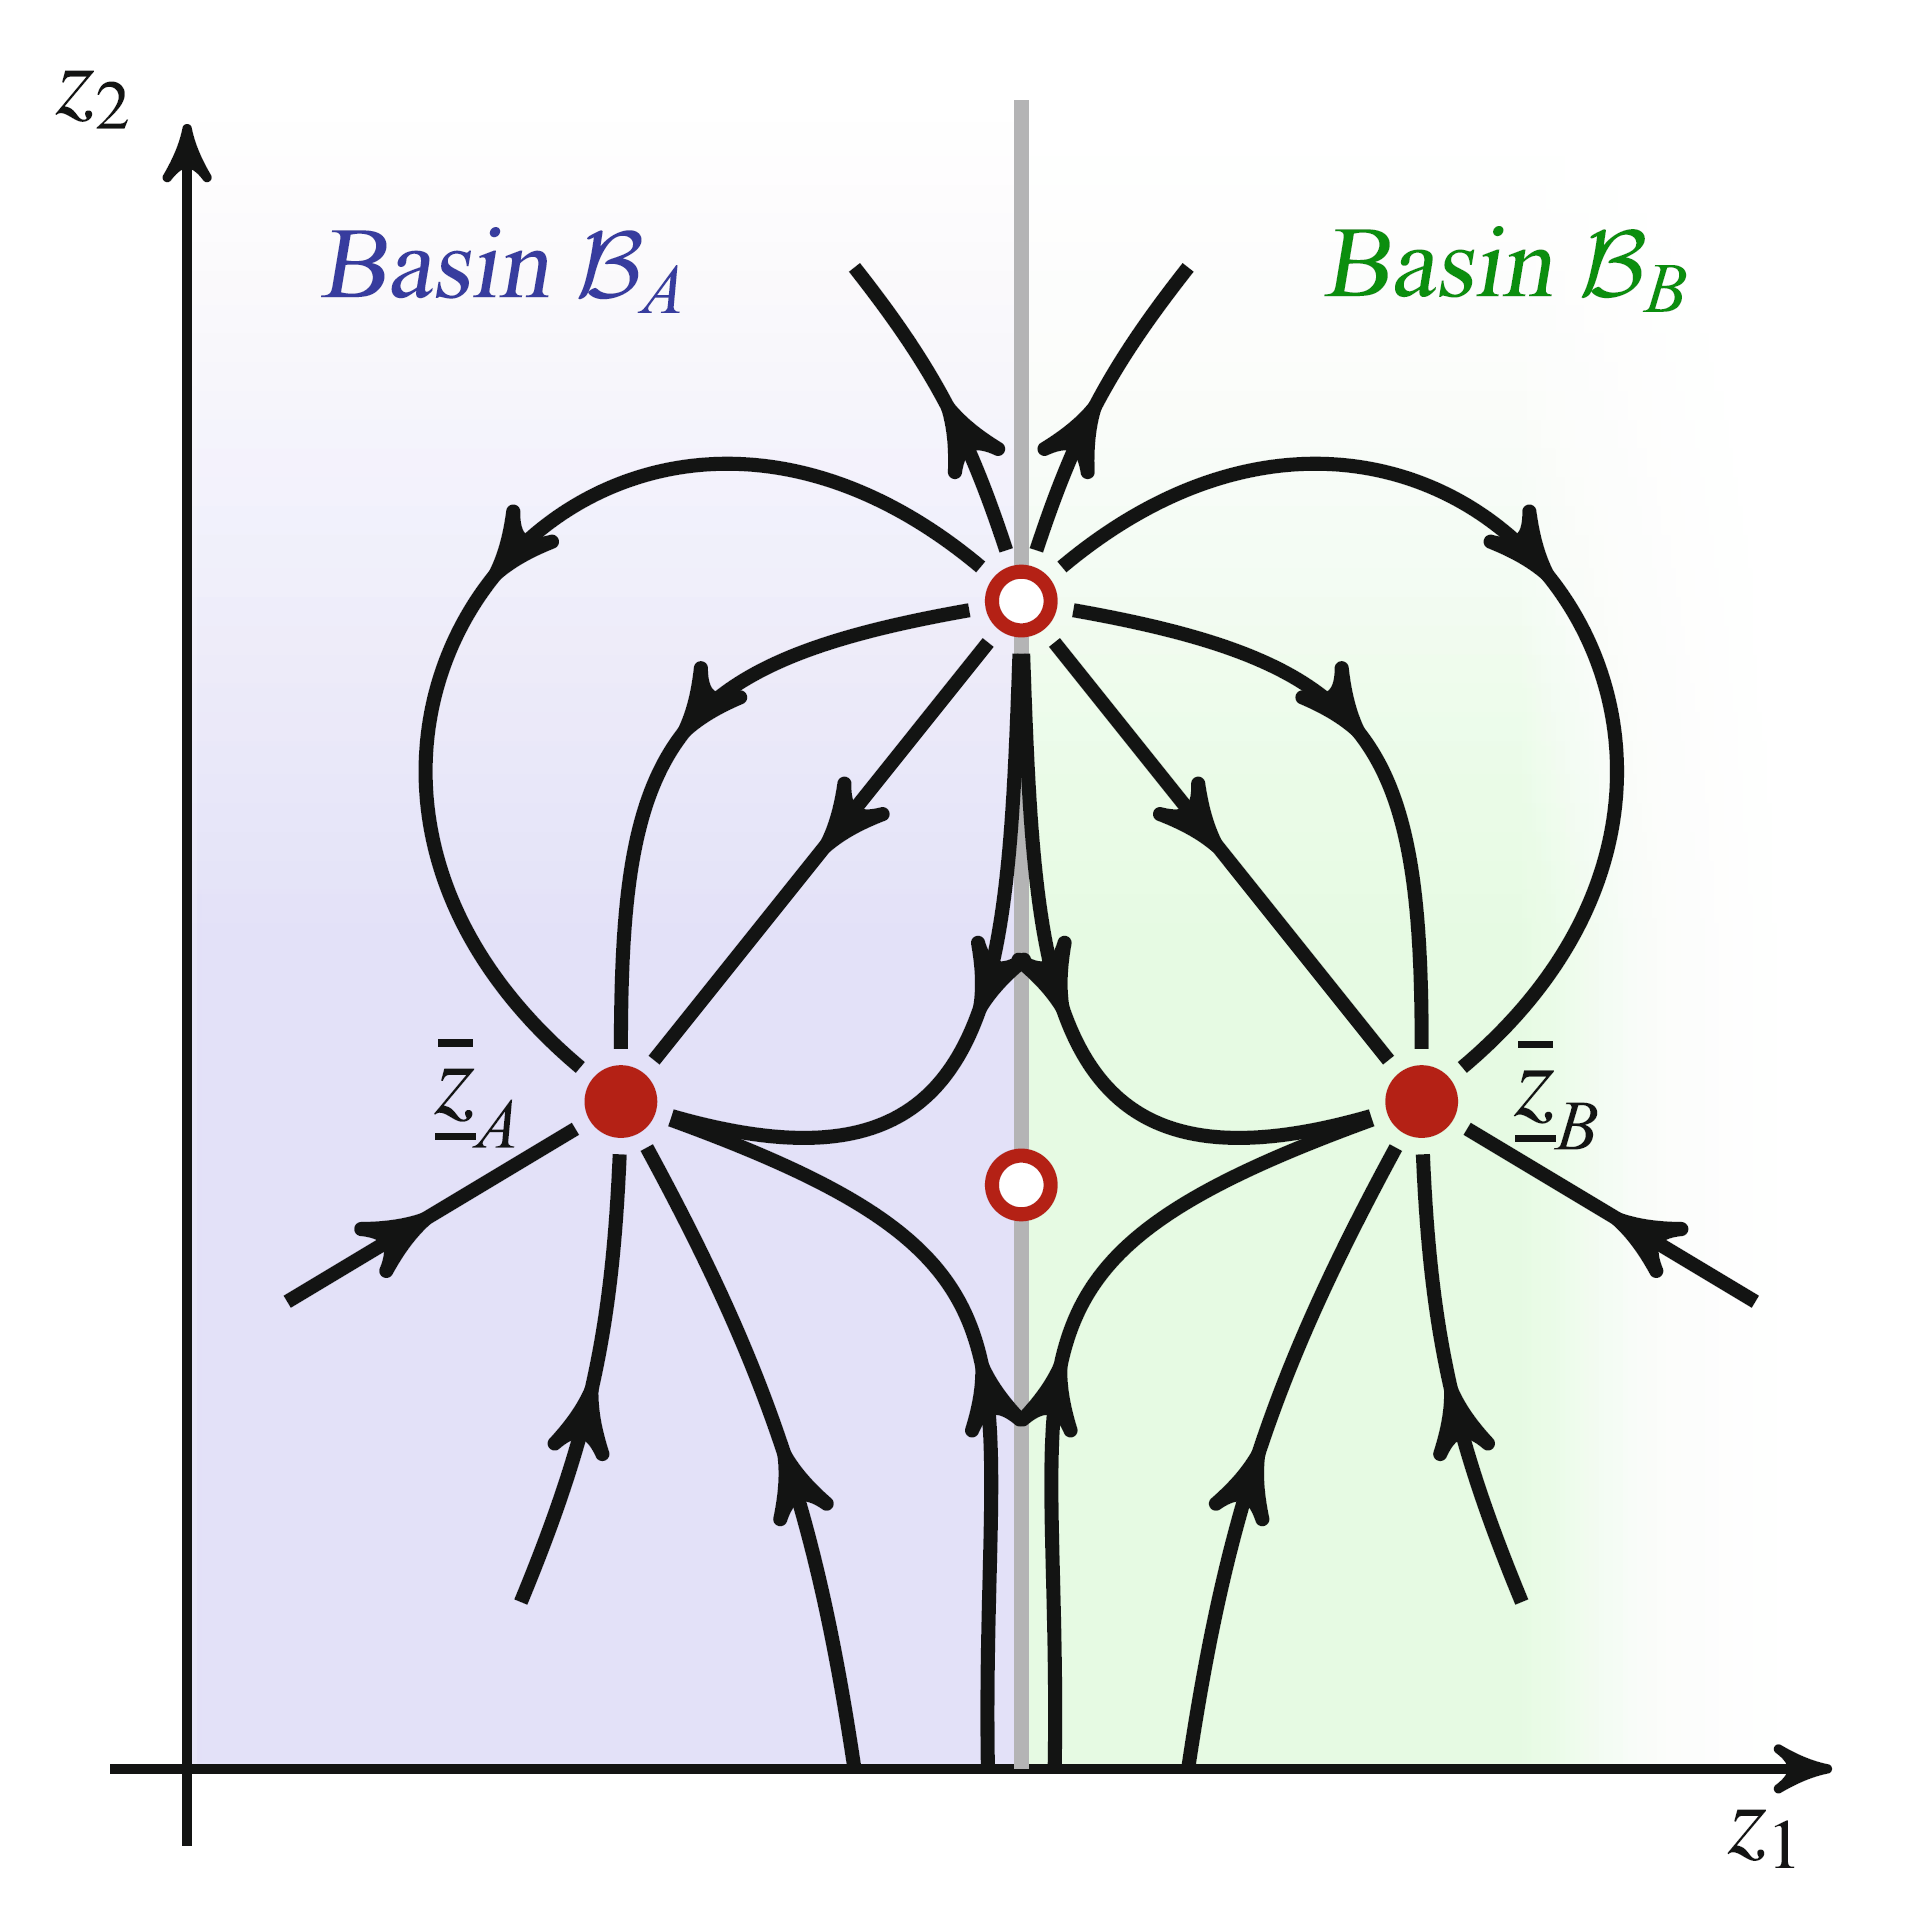
\includegraphics[width=\linewidth]{boa.png}
\end{wrapfigure}
A \emph{Basin of Attraction} describes that subset of the state space, such that initializing
the dynamics anywhere within the basin leads to convergence to a single
stable fixed point.
Thus all points $z$ in basin $\mathcal{B}_i$ converge to stable fixed point $\tilde{z}_i$.
\begin{equation}
	\mathcal{B}_i=\left\{z(0)\ \text{such that} \lim_{t\rightarrow\infty} z(t)=\tilde{z}_i \right\}
\end{equation}
\subsection{The Harmonic Oscillator}
\begin{equation}{\label{eq:tho}}
	\ddot{x}+\underbrace{\frac{\tilde{\gamma}}{m}}_{=2\gamma}\dot{x}+\underbrace{\frac{k}{m}}_{=\omega^2}x=0
\end{equation}
\subsubsection{Undamped Harmonic Oscillator}
If the damping constant vanishes, $\gamma=0$, (\ref{eq:tho}) simplifies to
\begin{equation}{\label{eq:bde2d}}
	\ddot{x}+\omega^2 x=0 
\end{equation}
The general solution of (\ref{eq:bde2d}) is given by
\begin{equation}
	x(t)=a\cos\omega t+b\sin\omega t
\end{equation}
In contrast to the first order systems we have dealt with so far, this general solution has not one but two free parameters, $a$ and $b$, that need to be determined from initial conditions.
\subsubsection{Damped Harmonic Oscillator}
\begin{equation}
	\ddot{x}+2\gamma\dot{x}+\omega^2x=0\quad\rightarrow\quad
	\begin{cases}
		\dot{x}=y\\
		\dot{y}=-\omega^2x-2\gamma y
	\end{cases}
\end{equation}
\begin{equation}
	\begin{pmatrix}
		\dot{x}\\\dot{y}
	\end{pmatrix}=
	\begin{pmatrix}
		0&1\\-\omega^2&-2\gamma
	\end{pmatrix}
	\begin{pmatrix}
		x\\y
	\end{pmatrix}
	\quad\rightarrow\quad
	\mathbf{\dot{x}}=A\mathbf{x}
\end{equation}
The eigenvectors are found from the relation
\begin{equation}
	A\mathbf{v}=\lambda\mathbf{v}\quad\rightarrow\quad
	\begin{pmatrix}
		0&1\\-\omega^2&-2\gamma
	\end{pmatrix}
	\begin{pmatrix}
		v_x\\v_y
	\end{pmatrix}=\lambda
	\begin{pmatrix}
		v_x\\v_y
	\end{pmatrix}
\end{equation}
\begin{equation}{\label{eq:dhos}}
	\rightarrow\quad\lambda_{1,2}=\left\{-\gamma\pm\sqrt{\gamma^2-\omega^2}\right\}
\end{equation}
By setting $v_x =1$, it is evident that oscillations can only occur if the eigenvalues have nonvanishing imaginary parts.
This means that the discriminant $\gamma^2-\omega^2$ in (\ref{eq:dhos}) must be smaller than zero.\\
Let $\gamma^2-\omega^2=-\Omega^2$ and $c=a+ib$.\\ 
The general solution  of (\ref{eq:tho}) is given by
\begin{equation}{\label{eq:gsho}}
	\begin{pmatrix}
		x(t)\\y(t)
	\end{pmatrix}=
	e^{-\gamma t}\left\{ce^{i\Omega t}
	\begin{pmatrix}
		1\\-\gamma+i\Omega
	\end{pmatrix}
	c^\ast e^{-i\Omega t}
	\begin{pmatrix}
		1\\-\gamma-i\Omega
	\end{pmatrix}\right\}
\end{equation}
which simplifies to 
\begin{equation}
	x(t)=e^{-\gamma t}\{a\cos\Omega t+b\sin\Omega t\}
\end{equation}
\begin{figure}[h!]
	\centering
	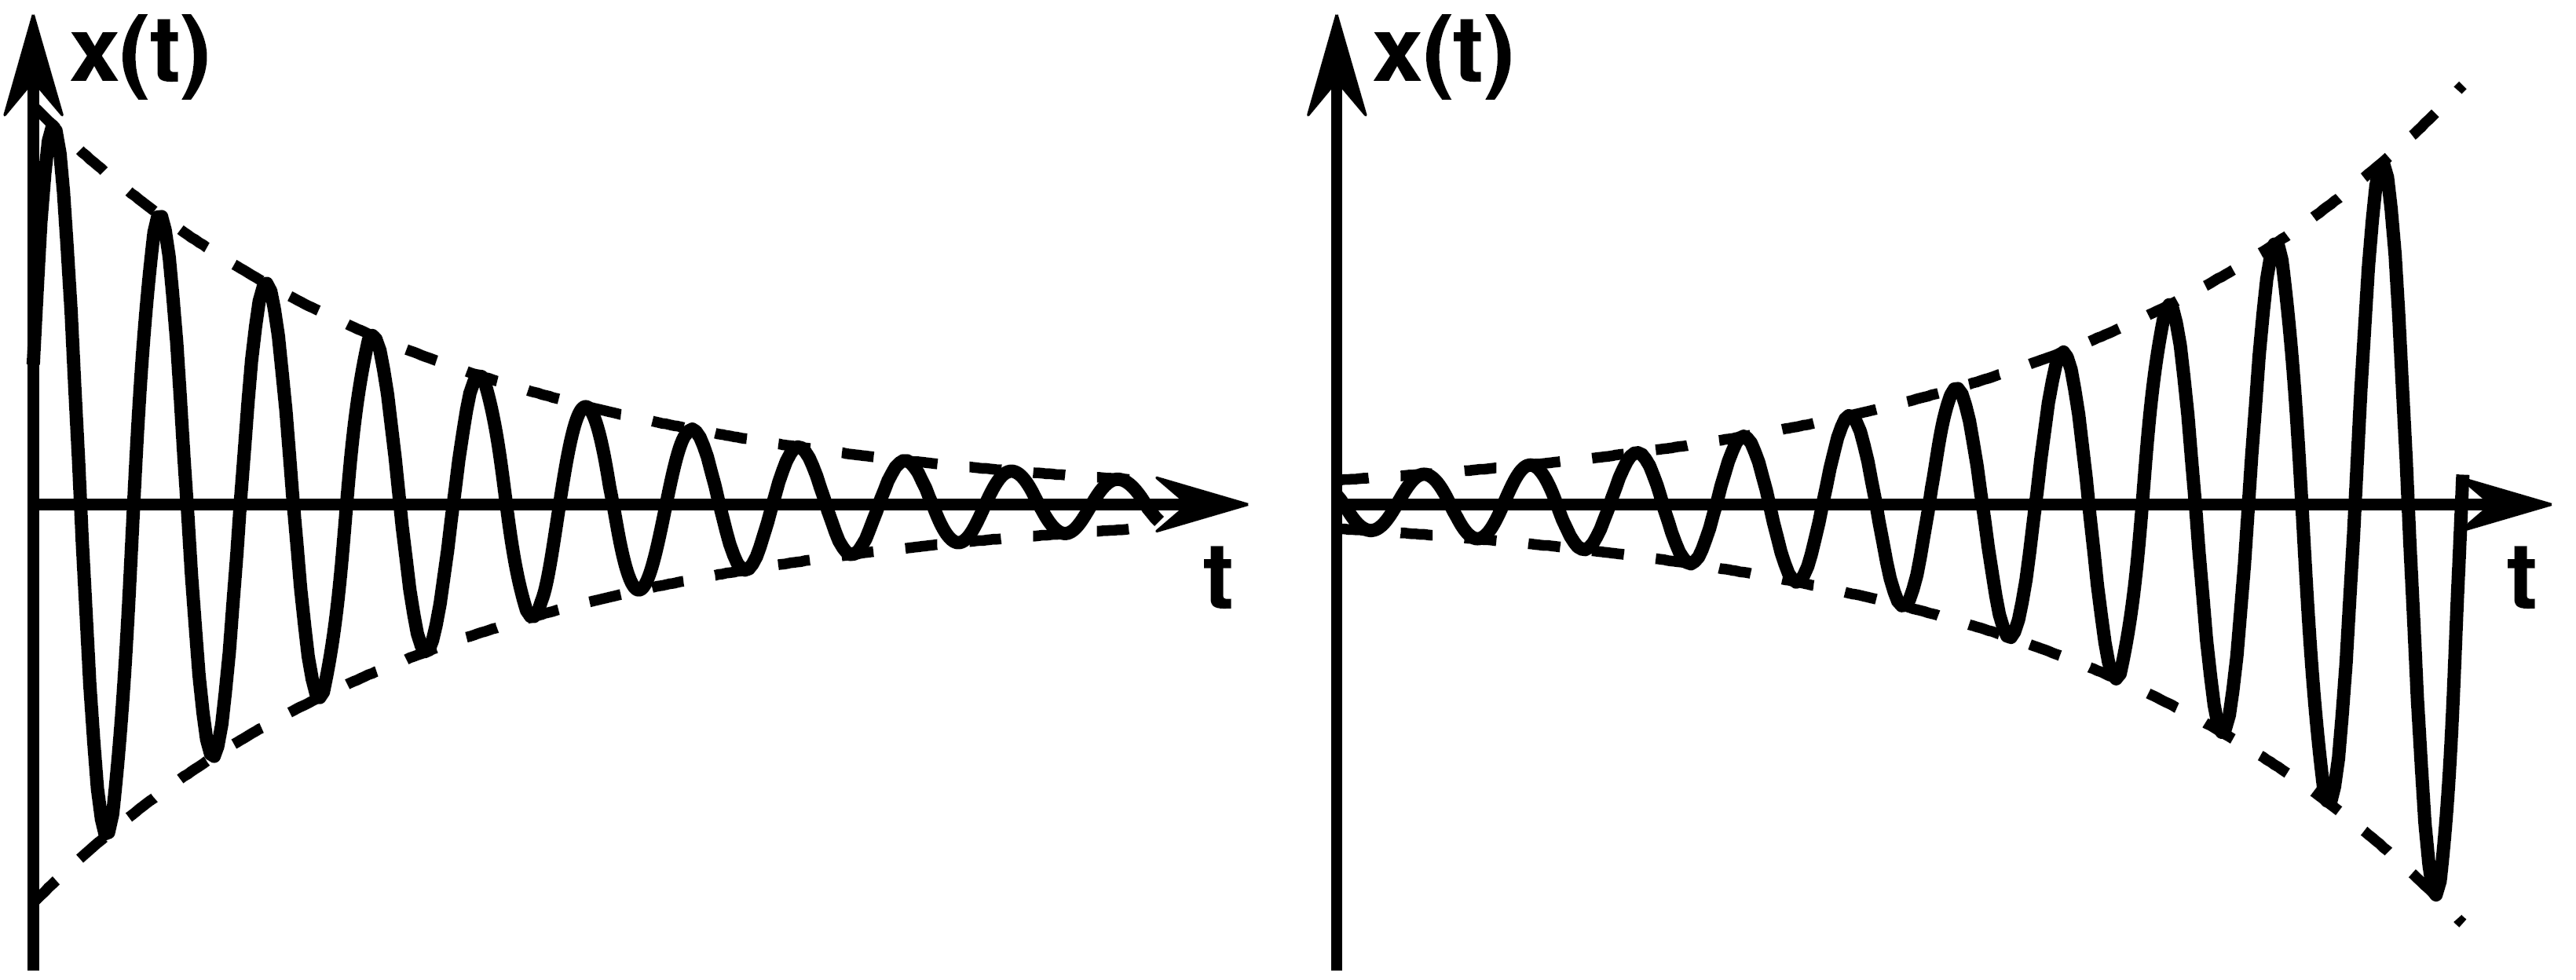
\includegraphics[width=0.5\linewidth]{dhs.png}
	\caption{Examples for damped harmonic oscillations for the case of positive damping $\gamma>0$ (left) and negative damping $\gamma>0$ (right).}
	\label{fig:dhs}
\end{figure}
If the damping constant $\gamma$ is greater than the angular velocity $\omega$ both eigenvalues are real numbers and the system does not oscillate. In this case equation (\ref{eq:gsho}) simplifies to 
\begin{equation}
	\begin{pmatrix}
		x(t)\\y(t)
	\end{pmatrix}=
	c_1e^{\lambda_1t}
	\begin{pmatrix}
		1\\\lambda_1
	\end{pmatrix}+
	c_2e^{\lambda_2t}
	\begin{pmatrix}
		1\\\lambda_2
	\end{pmatrix}\quad
	c_1,c_2\in\mathbb{R}
\end{equation}
which gives
\begin{equation}
	x(t)=c_1e^{\lambda_1t}+c_2e^{\lambda_2t}
\end{equation}
The solution is a superposition of two exponentials.

\section{Nonlinear Systems}
\subsection{Existence and Uniqueness Theorem}
We have no guarantee that the general nonlinear system $\mathbf{\dot{x}=f(x)}$ even has solutions! This theorem helps
\begin{theorem}[\textbf{Existence and Uniqueness Theorem}]{\label{thm:eut}}
	Consider the initial value problem $\mathbf{\dot{x}=f(x)}$, $\mathbf{x}(0)=\mathbf{x}_0$. Suppose that $\mathbf{f}$ is continuous and that all its partial derivatives $\partial f_i/\partial x_j, i,j=1,\ldots,n$ are continuous for $\mathbf{x}$ in some open connected set $D\subset\mathbb{R}^n$,
	then for $\mathbf{x}_0\in D$, the initial value problem has a solution $\mathbf{x}(t)$ on some time interval $(-\tau,\tau)$ about $t=0$, and the solution is unique.
\end{theorem}
\subsection{Linear Stability Analysis in Two Dimensions}
Nodes, stars, saddles, spirals and centers are the types of fixed points that exist in linear two-dimensional dynamical systems but they also allow for a classification of the fixed points and the dynamical behavior in their neighborhoods that are found in nonlinear systems.\footnote{The important \emph{Hartmann-Grobmann theorem} states that the phase space portrait in the neighborhood of a hyperbolic fixed point is topologically equivalent to its linearization. A fixed point is called \emph{hyperbolic} if none of the real parts of its eigenvalues vanish. Such points are also called \emph{structurally stable} and a small (infinitesimal) perturbation cannot change the topology of the phase space portrait in the vicinity of a hyperbolic fixed point.}\\
To achieve classification for the nonlinear case we have to perform a linear stability analysis\footnote{Also called \emph{Linearization}.} around the fixed points in two dimensions.
\begin{equation}
	\dot{x}=f(x,y),\quad\dot{y}=g(x,y)\quad\text{with a fixed point}\quad\mathbf{\tilde{x}}=
	\begin{pmatrix}
		\tilde{x}\\\tilde{y}
	\end{pmatrix}
\end{equation}
\begin{equation*}
	\rightarrow\quad f(\tilde{x},\tilde{y})=g(\tilde{x},\tilde{y})=0
\end{equation*}
We investigate the neighborhood of the fixed point by rewriting $x$ and $y$ in the form
\begin{equation}
	\mathbf{x}=
	\begin{pmatrix}
		x\\y
	\end{pmatrix}=
	\begin{pmatrix}
		\tilde{x}+\xi\\\tilde{y}+\eta
	\end{pmatrix}\quad\rightarrow\quad
	\begin{pmatrix}
		\dot{x}\\\dot{y}
	\end{pmatrix}=
	\begin{pmatrix}
		\dot{\xi}\\\dot{\eta}
	\end{pmatrix}=
	\begin{pmatrix}
		f(\tilde{x}+\xi, \tilde{y}+\eta)\\g((\tilde{x}+\xi, \tilde{y}+\eta)
	\end{pmatrix}
\end{equation}
We now expand $f(\tilde{x}+\xi, \tilde{y}+\eta)$ and $g(\tilde{x}+\xi, \tilde{y}+\eta)$ into a Taylor series
\begin{equation}
	\begin{aligned}
		\dot{\xi}=\underbrace{f(\tilde{x},\tilde{y})}_{=0}+\ \xi\at{\frac{\partial f(x,y)}{\partial x}}{\mathbf{x=\tilde{x}}}+\eta\at{\frac{\partial f(x,y)}{\partial y}}{\mathbf{x=\tilde{x}}}+O(\xi^2,\eta^2,\xi\eta)+\cdots\\
		\dot{\eta}=\underbrace{g(\tilde{x},\tilde{y})}_{=0}+\ \xi\at{\frac{\partial g(x,y)}{\partial x}}{\mathbf{x=\tilde{x}}}+\eta\at{\frac{\partial g(x,y)}{\partial y}}{\mathbf{x=\tilde{x}}}+O(\xi^2,\eta^2,\xi\eta)+\cdots
	\end{aligned}
\end{equation}
Truncating the expansion after the linear term.
In matrix notation this linearization reads
\begin{equation}{\label{eq:j2dnls}}
	\begin{pmatrix}
		\dot{\xi}\\\dot{\eta}
	\end{pmatrix}=
	\underbrace{
	\begin{pmatrix}
		\dfrac{\partial f}{\partial x}&\dfrac{\partial f}{\partial y}\\[10pt]
		\dfrac{\partial g}{\partial x}&\dfrac{\partial g}{\partial y}
	\end{pmatrix}
	}_{\text{Jacobian}}
	\begin{pmatrix}
		\xi\\\eta
	\end{pmatrix}
\end{equation}
With Equation (\ref{eq:j2dnls}), we can treat nonlinear systems by using methods of linear systems (Section (\ref{sec:cls})).
\subsubsection{The Effect of Small Nonlinear Terms}{\label{sec:eosnt}}
As long as the fixed point for the linearized system is not one of the borderline cases discussed in Figure (\ref{fig:sumls}) we can neglect nonlinear terms.
In other words, if the linearized system predicts a saddle, node, or a spiral, then the fixed point really is a saddle, node, or spiral for the original nonlinear system.
The borderline cases (centers, degenerate nodes, stars, or non-isolated fixed
points) can be altered by small nonlinear terms.
\subsection{Potential Functions in Two-Dimensional Systems}{\label{sec:pf2d}}
A two-dimensional system of first order differential equations of the form in Equation (\ref{eq:g2de}) has a potential and is called a gradient system if there exists a scalar function of two variables $V(x,y)$ such that
\begin{equation}
	\begin{pmatrix}
		\dot{x}\\\dot{y}
	\end{pmatrix}=
	\begin{pmatrix}
		f(x,y)\\g(x,y)
	\end{pmatrix}=-
	\begin{pmatrix}
		\dfrac{\partial V(x,y)}{\partial x}\\[10pt]
		\dfrac{\partial V(x,y)}{\partial y}
	\end{pmatrix}\quad\rightarrow\quad
	\mathbf{\dot{x}}=-\nabla V(x,y)\quad\text{with}\quad\nabla=
	\begin{pmatrix}
		\dfrac{\partial}{\partial x}\\[10pt]
		\dfrac{\partial}{\partial y}
	\end{pmatrix}
\end{equation}
As in the one-dimensional case the potential function $V(x,y)$ is monotonically decreasing as time evolves.
\begin{equation}
	\dot{V}(x,y)=\underbrace{\frac{\partial V}{\partial x}}_{-\dot{x}}\underbrace{\frac{\partial x}{\partial t}}_{\dot{x}}+
	\underbrace{\frac{\partial V}{\partial y}}_{-\dot{y}}\underbrace{\frac{\partial y}{\partial t}}_{\dot{y}}=-\dot{x}^2-\dot{y}^2=-|\mathbf{\dot{x}}|^2\leq0
\end{equation}
\begin{theorem}[\textbf{Existence of a Potential in Two-Dimensional Systems}]
	A \emph{potential} exists if and only if the relation
	\begin{equation}
		\frac{\partial f(x,y)}{\partial y}=\frac{\partial g(x,y)}{\partial x}
	\end{equation}
	is fulfilled.
\end{theorem}
\subsubsection{Separatrix}
A \textbf{separatrix} is an orbit that divides the phase plane into two distinctly different types of qualitative behavior.
The homoclinic and heteroclinic orbits are examples of separatrix cycles.
\paragraph{Homoclinic Orbit}
A closed trajectory that starts and ends at the same fixed point is correspondingly called a \emph{homoclinic orbit}.\\
Consider the system
\begin{equation}{\label{eq:ho}}
	\begin{aligned}
		\dot{x}&=y-y^2\\
		\dot{y}&=x
	\end{aligned}\quad\rightarrow\quad
	\mathbf{\tilde{x}}_1=
	\begin{pmatrix}
		0\\0
	\end{pmatrix}\quad
	\mathbf{\tilde{x}}_2=
	\begin{pmatrix}
		0\\1
	\end{pmatrix}
\end{equation}
with the Jacobian Matrix
\begin{equation}
	J=\begin{pmatrix}
		0&1-2y\\1&0
	\end{pmatrix}\quad\rightarrow\quad
	J(\mathbf{\tilde{x}}_{1,2})=
	\begin{pmatrix}
		0&\pm1\\1&0
	\end{pmatrix}
\end{equation}
At $(0,0)$, $t_r[J(\mathbf{\tilde{x}})]=0$ and $d_{et}[J({\mathbf{\tilde{x}}})]=-1$ so, origin is saddle point.\\
At $(0,1)$, $t_r[J(\mathbf{\tilde{x}})]=0$ and $d_{et}[J({\mathbf{\tilde{x}}})]=1$, it is center.\\
The trajectory leaves $\mathbf{\tilde{x_1}}$ along the unstable direction, curves around the center $\mathbf{\tilde{x_2}}$ and returns along the stable direction of the saddle (Figure (\ref{fig:ho})).
\begin{figure}[h!]
	\centering
	\begin{subfigure}{0.328125\linewidth}
		\centering
		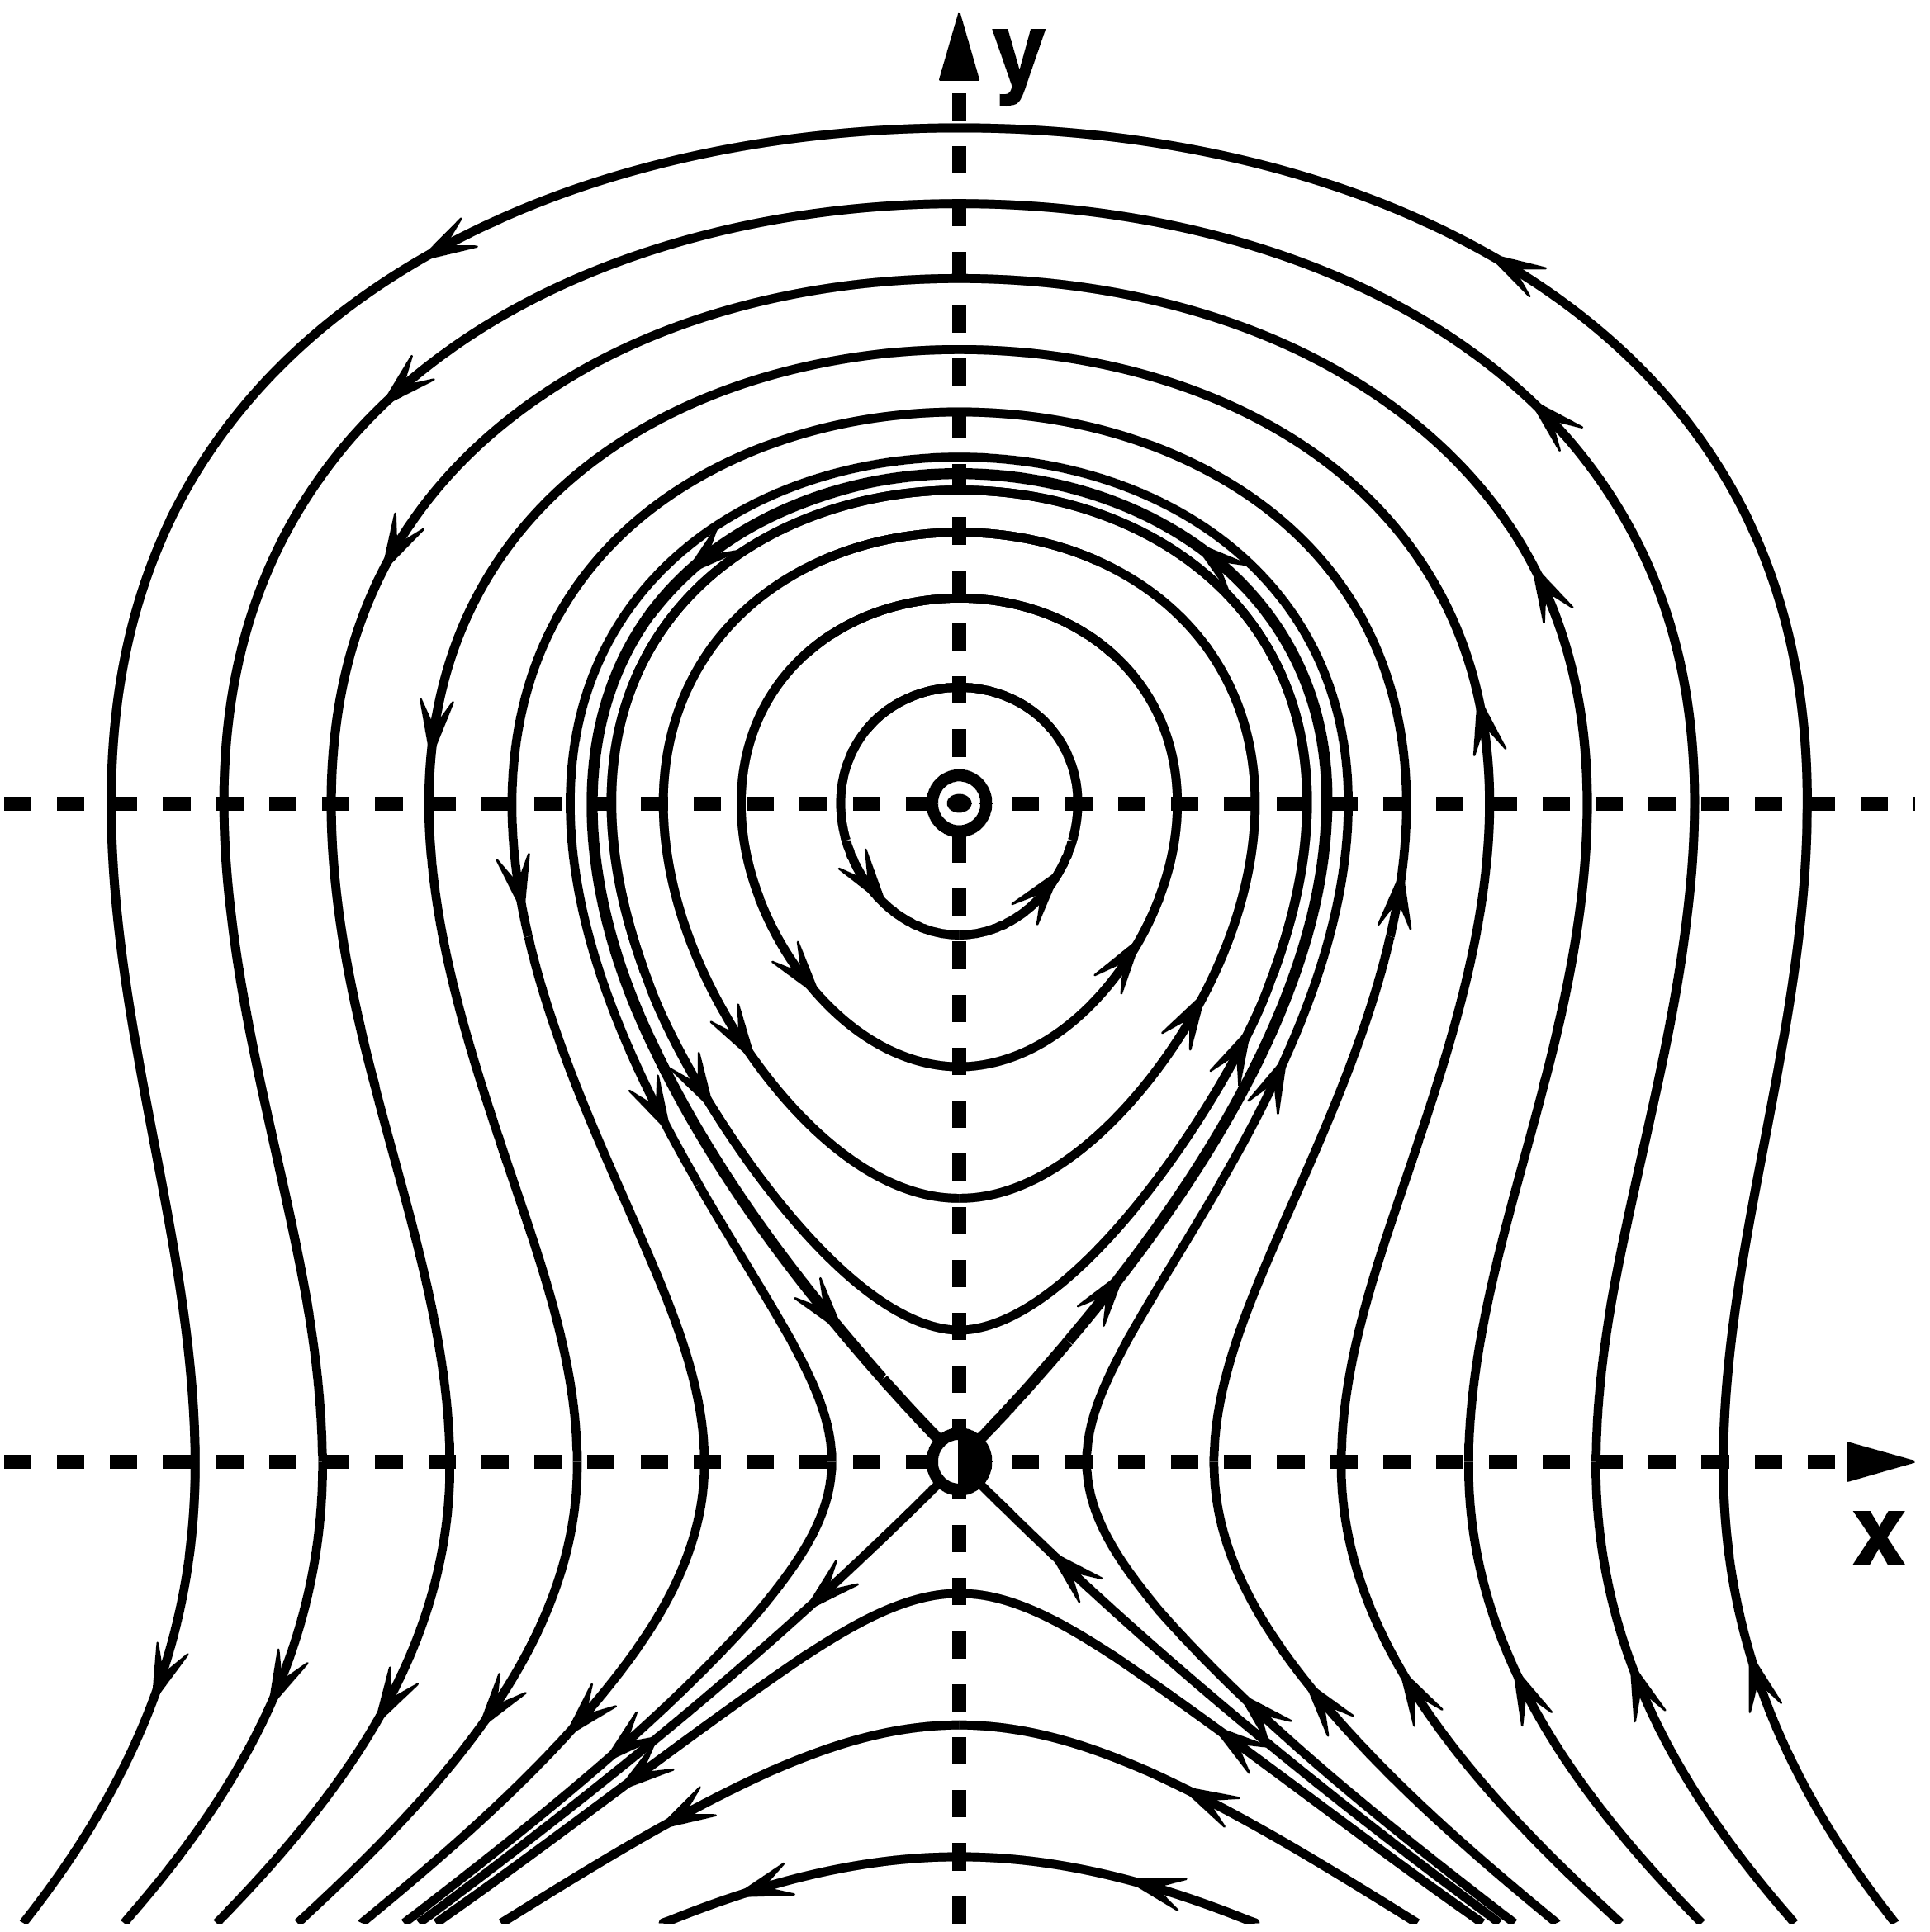
\includegraphics[width=\linewidth]{ho.png}
		\caption{Phase Space Plot of System (\ref{eq:ho})}
		\label{fig:ho}
	\end{subfigure}
	\vline
	\begin{subfigure}{0.35\linewidth}
		\centering
		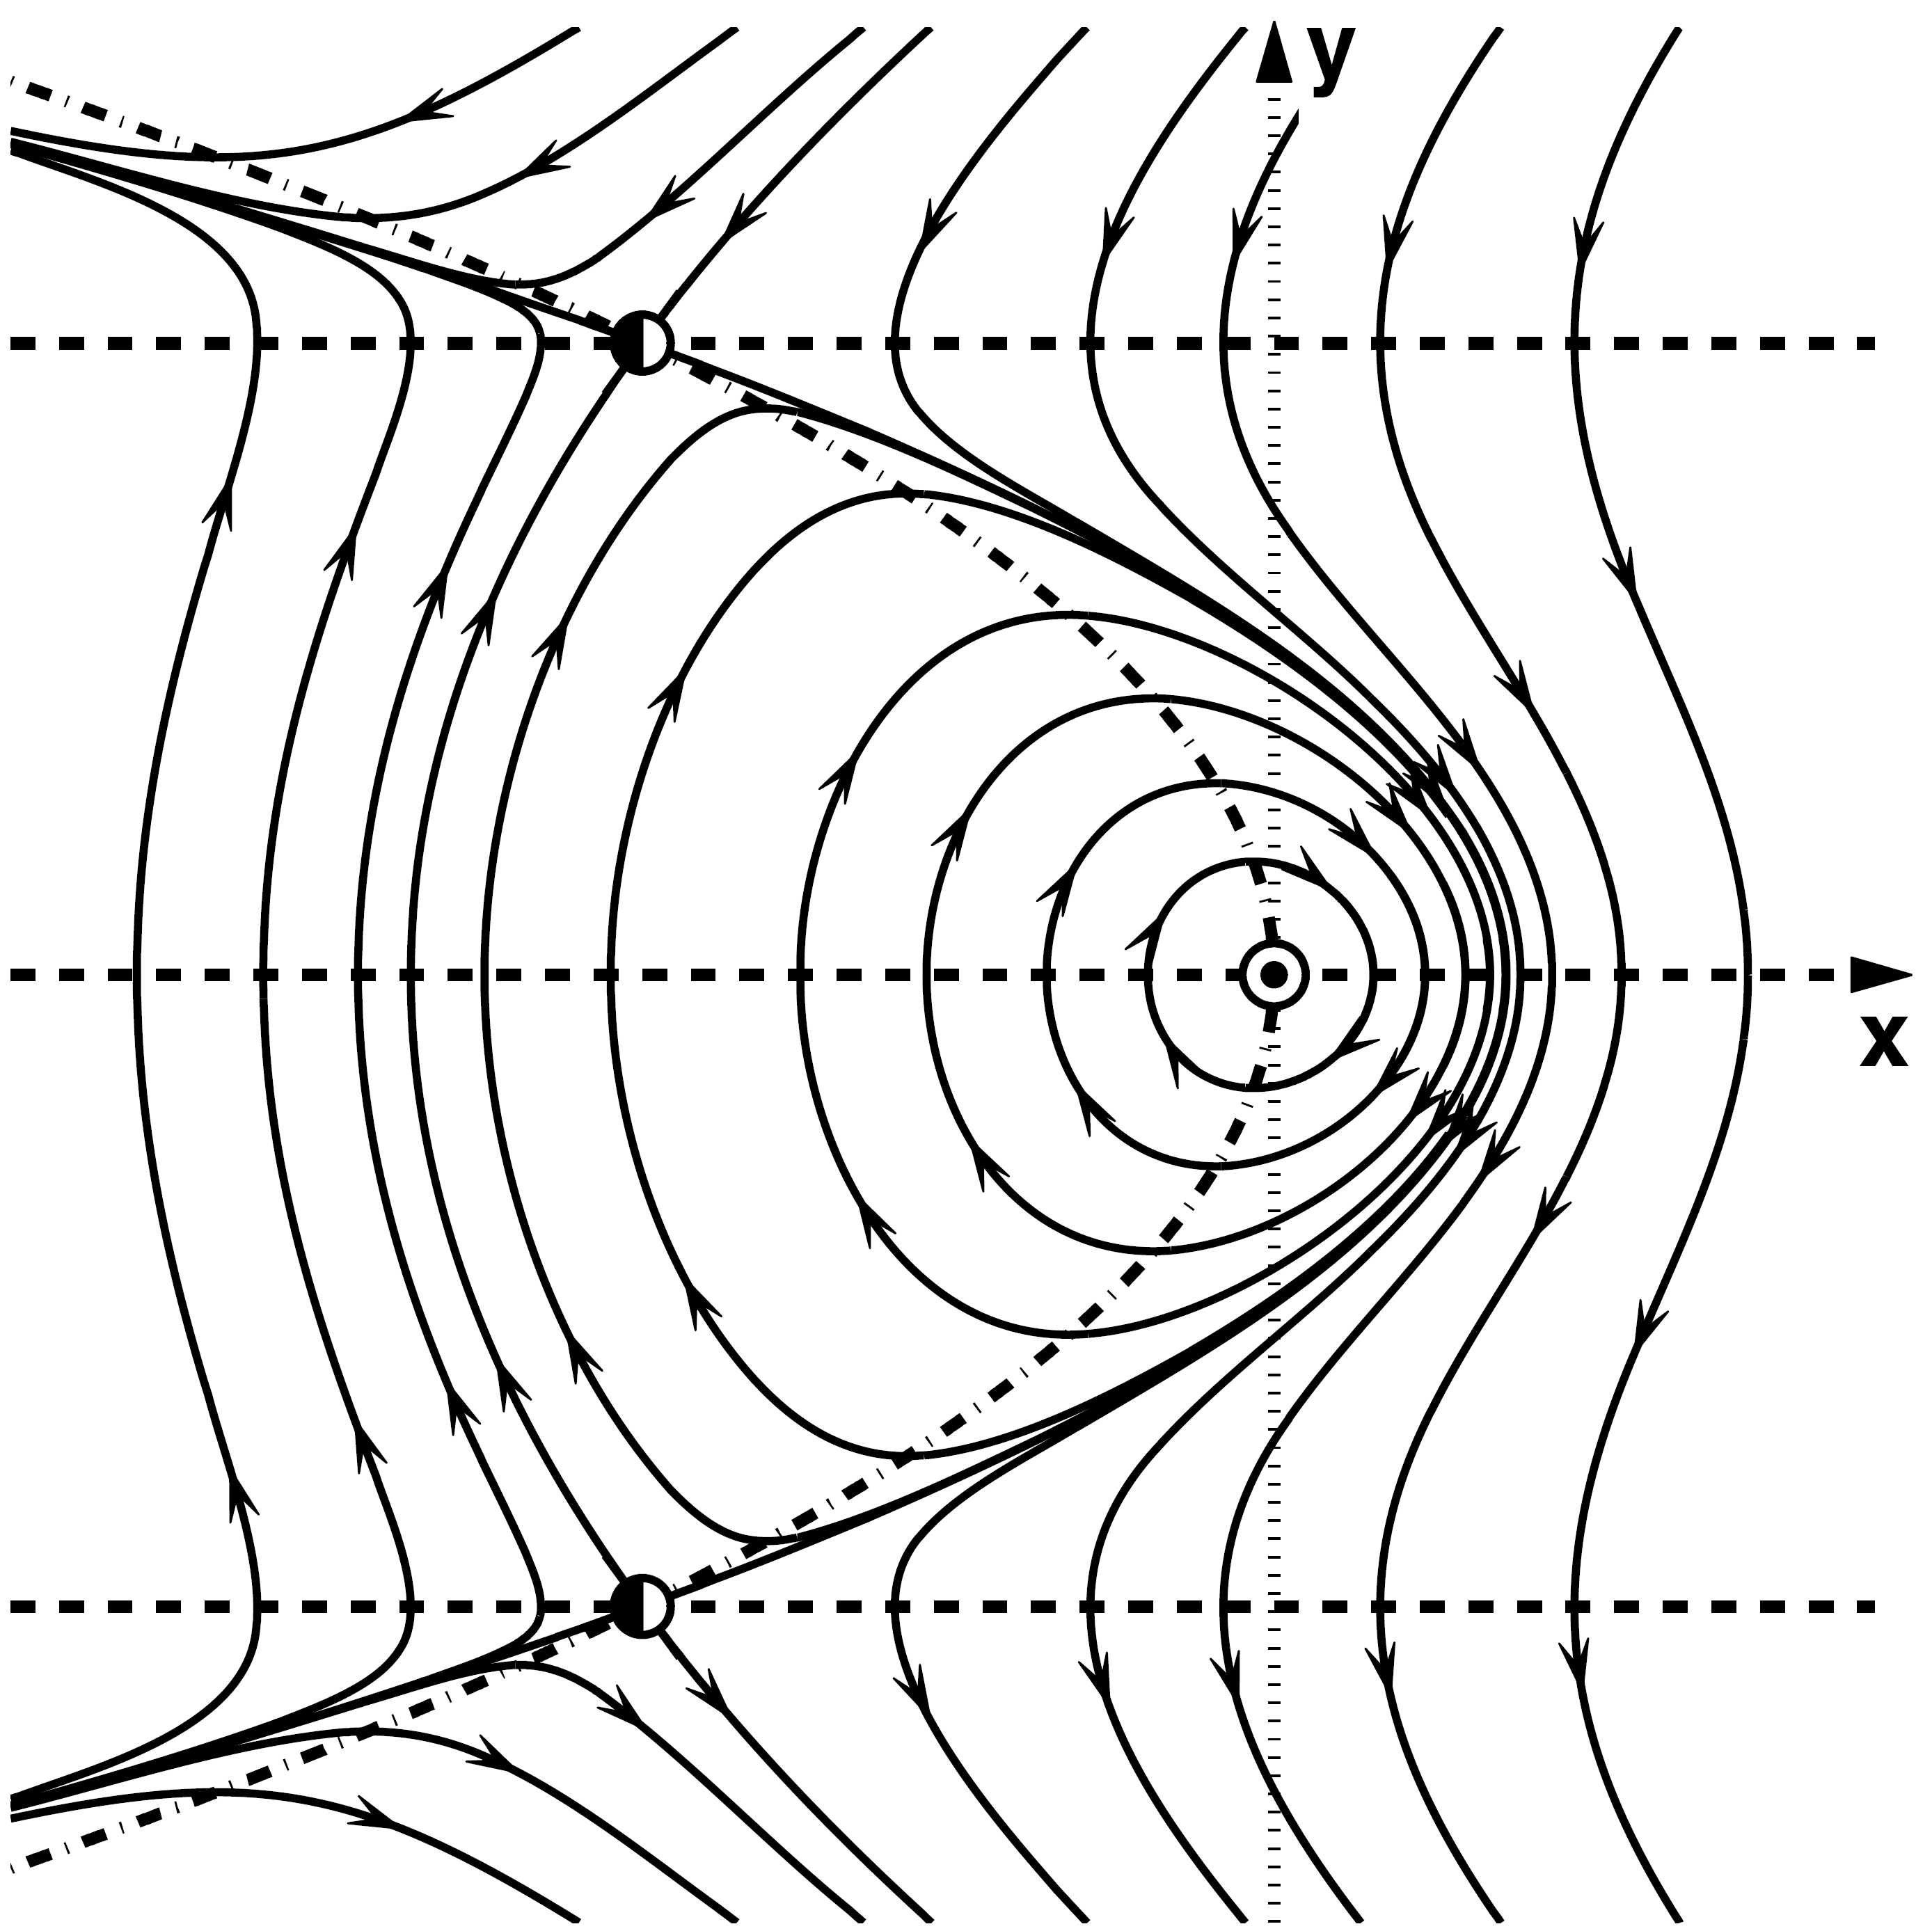
\includegraphics[width=\linewidth]{hto.png}
		\caption{Phase Space Plot of System with\\ \centering{$\dot{x}=y-y^3,\quad\dot{y}=-x-y^2$} }
		\label{fig:hto}
	\end{subfigure}
	\caption{Types of Orbits}
	\label{fig:nlo}
\end{figure}
\paragraph{Heteroclinic Orbit}
The trajectories connecting between two fixed points are called \emph{heteroclinic orbits} or \emph{saddle connections} (Figure (\ref{fig:hto})).
\subsection{Index Theory}
Linearization is a local method, it can’t tell us what happens to the trajectories after they leave that tiny neighborhood.
\emph{Index theory}, a method that provides global information about the phase portrait.
\subsubsection{The Index of a Closed Curve}
The index of a closed curve C is an integer that measures the winding of the
vector field on C.
The index also provides information about any fixed points that might happen to lie inside the curve.\\
Suppose that $\mathbf{\dot{x}=f(x)}$ is a smooth vector field on the phase plane.
Consider a closed curve $C$.
This curve is not necessarily a trajectory, it’s simply a loop that we’re putting in the phase plane to probe the behavior of the vector field.
We also assume that C is a “simple closed curve” (i.e., it doesn’t intersect itself) and that it doesn’t pass through any fixed points of the system.
Then at each point $\mathbf{x}$ on $C$, the vector field $\dot{x}=(\dot{x},\dot{y})$ makes angle $\phi=\tani(\dot{y}/\dot{x})$ with the positive $x-$axis.\\
As $\mathbf{x}$ moves counterclockwise around $C$, the angle $\phi$ changes \emph{continuously} since the vector field is smooth.
Also, when $\mathbf{x}$ returns to its starting place, $\phi$ returns to its original direction.
Hence, over one circuit, $\phi$ has changed by an integer multiple of $2\pi$. Let $[\phi]_C$ be the net change in $\phi$ over one circuit.
Then the \emph{index of the closed curve $C$ $(I_C)$} with respect to the vector field $\mathbf{f}$ is defined as
\begin{equation}
	I_C=\frac{1}{2\pi}[\phi]_C
\end{equation}
Thus, $I_C$ is the net number of counterclockwise revolutions made by the vector field as $\mathbf{x}$ moves once counterclockwise around $C$.
\subsubsection{Index of a Point}
Suppose $\mathbf{\tilde{x}}$ is an isolated fixed point.
Then the index $I$ of $\mathbf{\tilde{x}}$ is defined as $I_C$, where $C$ is any closed curve that encloses $\mathbf{\tilde{x}}$ and no other fixed points.
By property (1) below, $I_C$ is independent of $C$ and is therefore a property of $\mathbf{\tilde{x}}$ alone.
\begin{itemize}
	\item The index $I=+1$ for stable node, unstable node, spirals, centers, degenerate nodes and stars.
	\item The index $I=-1$ for saddle.
\end{itemize}
\subsubsection{Properties of the Index}
\begin{itemize}
	\item Suppose that $C$ can be continuously deformed into $C^\prime$ without passing through a fixed point.
	Then $I_C=I_{C^\prime}$
	\item If $C$ doesn’t enclose any fixed points, then $I_C=0$.
	\item If we reverse all the arrows in the vector field by changing $t\rightarrow-t$, the index is unchanged.
	Therefore, the index is not related to stability.
	\item Suppose that the closed curve $C$ is actually a trajectory for the system, i.e., $C$ is a closed orbit.
	Then $I_C=1$.
\end{itemize}
\begin{theorem}
	If a closed curve $C$ surrounds $n$ isolated fixed points $\mathbf{\tilde{x}}_1,\ldots,\mathbf{\tilde{x}}_n$ then
	\begin{equation}
		I_C=I_1+I_2+\cdots+I_n
	\end{equation}
	Where $I_k$ is the index of $\mathbf{\tilde{x}}_k$, for $k=1,\ldots,n$
\end{theorem}
\begin{theorem}
	Any closed orbit in the phase plane must enclose fixed points whose \emph{indices sum to} $+1$.
\end{theorem}

\section{Conservative Systems}
Systems for which a conserved quantity exists are called \textbf{conservative systems}.\\\\
Given a system $\mathbf{\dot{x}}=\mathbf{f}(\mathbf{x})$, a conserved quantity is a real-valued continuous function $E(\mathbf{x})$ that is constant on trajectories, i.e. $\dfrac{dE}{dt}=0$ and $E(\mathbf{x})$ be nonconstant on every open set.
\begin{theorem}
	A conservative system cannot have any attracting fixed points.
\end{theorem}
\begin{proof}
	Suppose $\mathbf{\tilde{x}}$ were an attracting fixed point.
	Then all points in its basin of attraction would have to be at the same energy $E(\mathbf{\tilde{x}}$) (because energy is constant on trajectories and all trajectories in the basin flow to $\mathbf{\tilde{x}}$).
	Hence $E(\mathbf{x})$ must be a constant function for $\mathbf{x}$ in the basin.
	But this contradicts our definition of a conservative system, in which we required that $E(\mathbf{x})$ be nonconstant on all open sets.
\end{proof}
\subsection*{Nonlinear Centers}
Centers are ordinarily very delicate (See Section (\ref{sec:eosnt})), they are much more robust when the system is conservative.
\begin{theorem}[\textbf{Nonlinear centers for conservative systems}]
	Consider the system $\mathbf{\dot{x}}=\mathbf{f}(\mathbf{x})$, and $\mathbf{f}$ is continuously differentiable.
	Suppose there exists a conserved quantity $E(\mathbf{x})$ and suppose that $\mathbf{\tilde{x}}$ is an isolated fixed point (i.e., there are no other fixed points in a small neighborhood surrounding $\mathbf{\tilde{x}}$).
	If $\mathbf{\tilde{x}}$ is a local minimum of $E$, then all trajectories sufficiently close to $\mathbf{\tilde{x}}$ are closed.
\end{theorem}

\section{Reversible Systems}
Many mechanical systems have time-reversal symmetry.
This means that their dynamics look the same whether time runs forward or backward.
A second-order system \emph{reversible system} is invariant under $t\rightarrow-t$ and $y\rightarrow-y$.
\begin{equation}{\label{eq:rs2d}}
	\begin{aligned}
		\dot{x}&=f(x,y)\\
		\dot{y}&=g(x,y)
	\end{aligned}
\end{equation}
where $f$ is odd in $y$ and $g$ is even in $y$.
\subsection*{Nonlinear Centers}
\begin{theorem}[\textbf{Nonlinear centers for reversible systems}]
	Suppose the origin $\mathbf{\tilde{x}}=\mathbf{0}$ is a linear center for the reversible continuously differentiable system (\ref{eq:rs2d}).
	Then sufficiently close to the origin, all trajectories are \textbf{closed curves}.
\end{theorem}

\section{Limit Cycles}{\label{sec:lc}}
A limit cycle is an \emph{isolated closed trajectory}.
\emph{Isolated} means that neighboring trajectories are not closed; they spiral either toward or away from the limit cycle.
\begin{figure}[H]
	\centering
	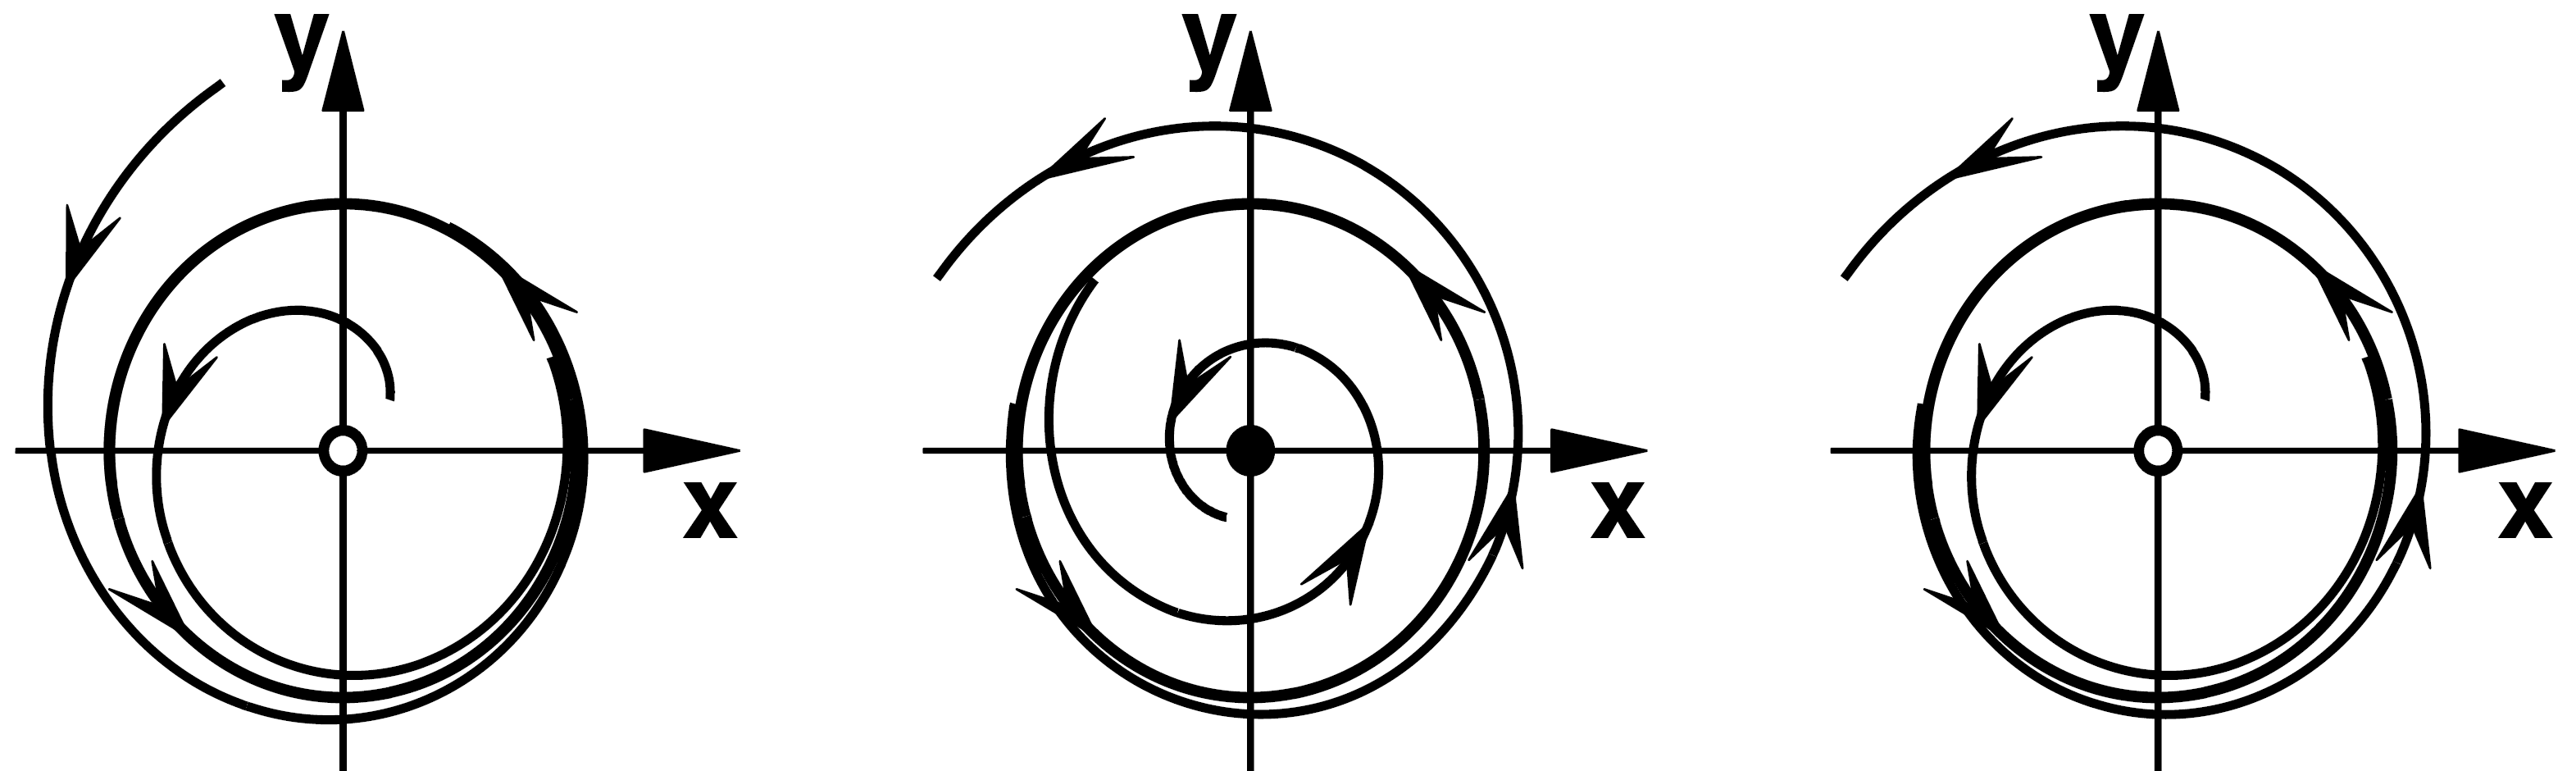
\includegraphics[width=0.5\linewidth]{tlc.png}
	\caption{Limit cycles attracting or/and repelling neighboring trajectories. Stable (right), unstable (middle), half-stable (right)}
	\label{fig:tlc}
\end{figure}
A \emph{stable} limit cycle attracts trajectories from its outside and its inside, whereas an \emph{unstable} limit cycle repels trajectories on both sides.
A \emph{half-stable} limit cycle attract the trajectories from one side and repel those on the other.\\
It is intuitively clear that inside a stable limit cycle there must be an unstable fixed point and vic-versa (Figure (\ref{fig:tlc})).
\subsection{Closed Orbits}
\begin{theorem}[\textbf{Gradient System}]
	\emph{Closed orbits and Limit Cycles are impossible} if the systems can be written in the form $\mathbf{\dot{x}}=-\nabla V$ for some continuously differentiable, single-valued scalar function $V(x)$. 
\end{theorem}
\begin{proof}
	Suppose there were a closed orbit. We obtain a contradiction by considering the change in $V$ after one circuit.
	On the one hand, $\Delta V=0$ since $V$ is single-valued.
	But on the other hand,
	\begin{equation}
		\Delta V=\int_0^T\frac{dV}{dt}\mathop{dt}=\int_0^T(\Delta V\cdot\mathbf{\dot{x}})\mathop{dt}=-\int_0^T\|\mathbf{\dot{x}}\|^2\mathop{dt}<0 
	\end{equation}
	If $\mathbf{\dot{x}}=0$ the trajectory is a fixed point, not a closed orbit.
	This contradiction shows that closed orbits can’t exist in gradient systems. 
\end{proof}
\begin{theorem}[\textbf{Lyapunov Function}]
	Consider Case 2. of Theorem (\ref{thm:lst}).\\
	Here $\mathbf{\tilde{x}}$ is globally asymptotically stable: for all initial conditions, $\mathbf{x}(t)\rightarrow\mathbf{\tilde{x}}$ as $t\rightarrow\infty$.\\
	In particular the system has \emph{no closed orbits}.
\end{theorem}
\begin{theorem}[\textbf{Bendixson’s Negative Criterion}]
	There are \emph{no closed paths} in a simply connected region of the phase plane of the system on which $\left(\dfrac{\partial f_1}{\partial x_1}+\dfrac{\partial f_2}{\partial x_2}\right)$ is not identically zero and is of one sign.
\end{theorem}
\begin{theorem}[\textbf{Dulac’s Criterion}]
	Let $\mathbf{\dot{x}}=\mathbf{f(x)}$ be a continuously differentiable vector field defined on a simply connected subset $R$ of the plane.
	If there exists a continuously differentiable, real-valued function $g(\mathbf{x})$ such that $\nabla\cdot(g\mathbf{\dot{x}})$ has one sign throughout $R$, then there are \emph{no closed orbits} lying entirely in $R$.
\end{theorem}
\begin{proof}
	Suppose there were a closed orbit $C$ lying entirely in the region $R$. Let $A$ denote the region inside $C$. Then Green’s theorem yields
	\begin{equation}
		\iint_A\nabla\cdot(g\mathbf{\dot{x}})\mathop{dA}=\oint_Cg\mathbf{\dot{x}}\cdot\mathbf{n}\mathop{d\ell}
	\end{equation}
	Where $\mathbf{n}$ is the outward normal and $d\ell$ is the element of arc length along $C$.
	Look first at the double integral on the left: it must be \emph{nonzero}, since $\nabla\cdot(g\mathbf{\dot{x}})$ has one sign in $R$.
	On the other hand, the line integral on the right equals \emph{zero} since $\mathbf{\dot{x}}\cdot\mathbf{n}=0$ everywhere, by the assumption that $C$ is a trajectory (the tangent vector $\mathbf{\dot{x}}$ is orthogonal to $\mathbf{n}$).
	This contradiction implies that no such $C$ can exist.
\end{proof}
The following theorem gives the criterion for a system to have finite number of limit cycles.
\begin{theorem}[\textbf{Dulac}]
	In any bounded region of the plane, a planar analytic system $\dot{x}=f(x)$ analytic in $\mathbb{R}^2$ has at most a finite number of limit cycles.
	In other words, any polynomial system has at most a finite number of limit cycles in $\mathbb{R}^2$.
\end{theorem}
\begin{theorem}[\textbf{Poincar\'e}]
	A planar analytic system (\ref{eq:2d}) cannot have an infinite number of limit cycles that accumulate on a cycle of (\ref{eq:2d}).
\end{theorem}
\subsection{Poincar\'e--Bendixson Theorem}
This theorem helps in finding methods to establish that closed orbits exist in particular systems.
\begin{wrapfigure}{r}{0.3\textwidth}
	\centering
	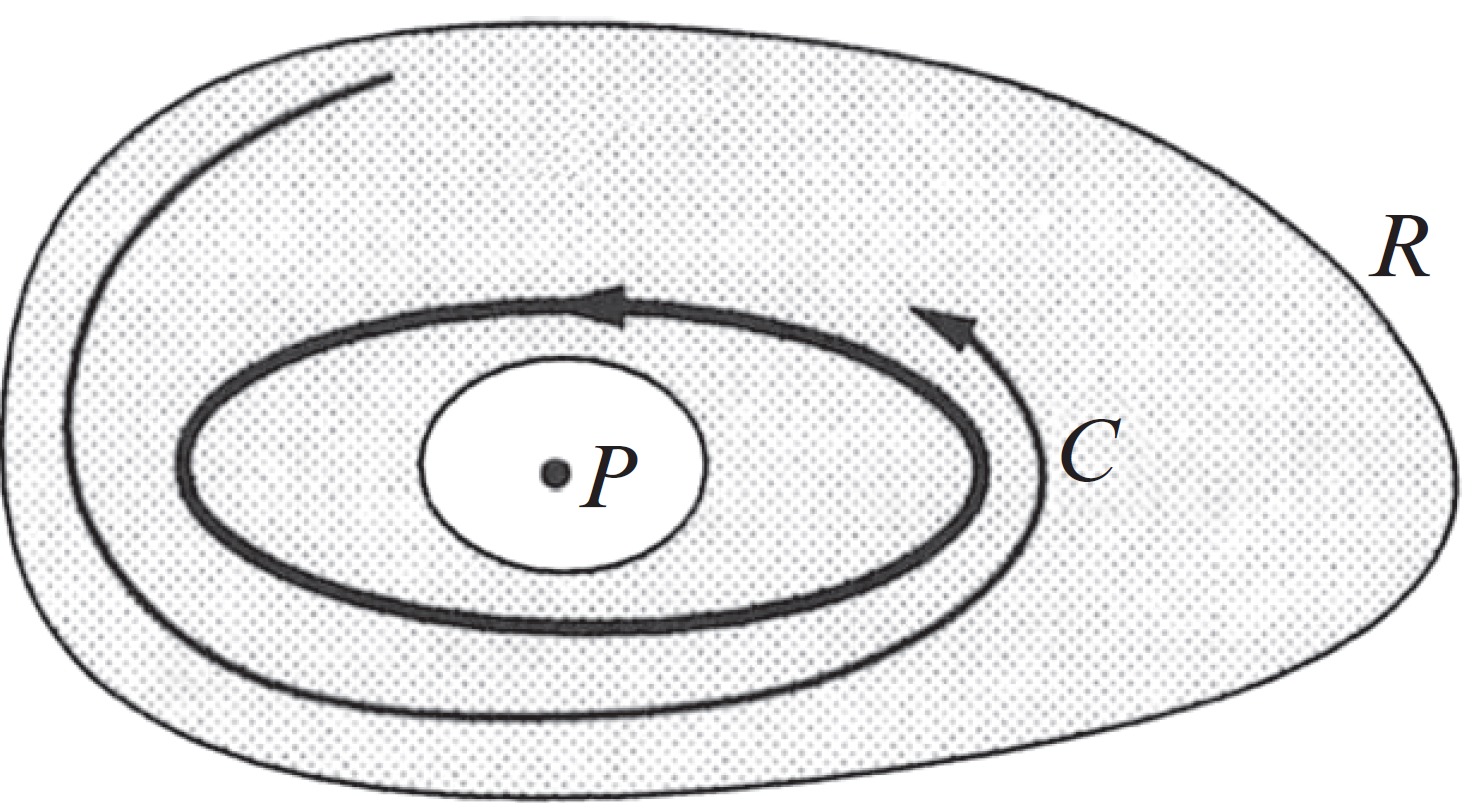
\includegraphics[width=0.25\textwidth]{pbt.png}
	\caption{}
	\label{fig:pbt}
\end{wrapfigure}
\begin{theorem}[\textbf{Poincar\'e--Bendixson Theorem}]
	Suppose that:
	\begin{itemize}
		\item $R$ is a closed, bounded subset of the plane.
		\item $\mathbf{\dot{x}=f(x)}$ is a continuously differentiable vector field on an open set containing $R$.
		\item $R$ does not contain any fixed points.
		\item There exists a trajectory $C$ that is \emph{confined}in $R$, in the sense that it starts in $R$ and stays in $R$ for all future time (Figure (\ref{fig:pbt})).
	\end{itemize}
	Then either $C$ is a closed orbit, or it spirals toward a closed orbit as $t\rightarrow\infty$.
	In either case, \emph{$R$ contains a closed orbit} (shown as a heavy curve in Figure (\ref{fig:pbt})). 
\end{theorem}

\section{Nonlinear Oscillators}
\subsection{Li\'enard System}
Consider the system
\begin{equation}{\label{eq:nols}}
	\begin{aligned}
		\dot{x}&=y-F(x)\\
		\dot{y}&=-g(x)
	\end{aligned}\quad\rightarrow\quad
	\ddot{x}+f(x)\dot{x}+g(x)=0\quad(f(x)=F^\prime(x))
\end{equation}
\begin{theorem}[\textbf{Li\'enard Theorem}]
	Suppose two functions $f(x)$ and $g(x)$ satisfy the following conditions
	\begin{itemize}
		\item $f(x)$ and $g(x)$ are continuously differentiable for all $x$
		\item $g(-x)=-g(x)\ \forall\ x$, i.e. $g(x)$ is an odd function
		\item $g(x)>0$ for $x>0$
		\item $f(-x)=f(x)\ \forall\ x$, i.e. $f(x)$ is an even function
		\item The odd function, $F(x)=\displaystyle\int_0^xf(u)du$, has exactly one positive zero at $x=\alpha$ (say), $F(x)$ is negative for $0<x<\alpha$, and $F(x)$ is positive and nondecreasing for $x>\alpha$ and $F(x)\rightarrow\infty$ as $x\rightarrow\infty$.
	\end{itemize}
	Then the Li\'enard equation \emph{(\ref{eq:nols})} has a \emph{\textbf{unique stable limit cycle}} surrounding the origin of the phase plane.
\end{theorem}
The Li\'enard system is a very special type of equation that has a unique stable
limit cycle.\\\\
Equation of Nonlinear Oscillators are given by introducing nonlinear terms in Equation (\ref{eq:tho})
\begin{equation}{\label{eq:nlo}}
	\ddot{x}+\gamma\dot{x}+\omega^2x+N(x,\dot{x})=0
\end{equation}
\subsection{Van-der-Pol Oscillator: $N(x,\dot{x}=x^2\dot{x})$}
The van-der-Pol oscillator is given by
\begin{equation}{\label{eq:vdpo}}
	\ddot{x}+\gamma\dot{x}+\omega^2x+\epsilon x^2\dot{x}=0\quad\rightarrow\quad
	\ddot{x}+\underbrace{(\gamma+\epsilon x^2)}_{\tilde{\gamma}}\dot{x}+\omega^2x=0
\end{equation}
Equation (\ref{eq:vdpo}) shows that for the van-der-Pol oscillator the damping ‘constant’ $\tilde{\gamma}$ becomes time dependent via the amplitude $x^2$.
\begin{itemize}
	\item $\gamma>0\quad\epsilon>0$\\ The effective damping $\tilde{\gamma}$ is always positive.
	The trajectories are evolving towards the origin, which is a stable fixed point.
	\item $\gamma<0\quad\epsilon<0$\\ The effective damping $\tilde{\gamma}$ is always negative.
	The system is unstable and the trajectories are evolving towards infinity.
	\item $\gamma>0\quad\epsilon<0$\\ For small values of the amplitude $x^2$ the effective damping $\tilde{\gamma}$ is positive leading to even smaller amplitudes.
	For large values of $x^2$ the effective damping $\tilde{\gamma}$ is negative leading a further increase in amplitude.
	The system evolves either towards the fixed point or towards infinity depending on the initial conditions.
	\item $\gamma<0\quad\epsilon>0$\\ For small values of the amplitude $x^2$ the effective damping $\tilde{\gamma}$ is negative leading to an increase in amplitude.
	For large values of $x^2$ the effective damping $\tilde{\gamma}$ is positive and the amplitude decreases.
	The system evolves towards a stable limit cycle.
	Without the nonlinearity the system is unstable $(\gamma<0)$ (Figure (\ref{fig:dhs}) right) and moves away from the fixed point at the origin.
	As the amplitude increases the nonlinear damping $(\epsilon>0)$ becomes an important player and leads to saturation of the amplitude at a finite value.
\end{itemize}
The time series is not a sine function but has a fast rising increasing flank and a more shallow slope on the decreasing side. Such time series are called \textbf{relaxation oscillations}.
\begin{figure}[h!]
	\centering
	\begin{subfigure}{0.45\linewidth}
		\centering
		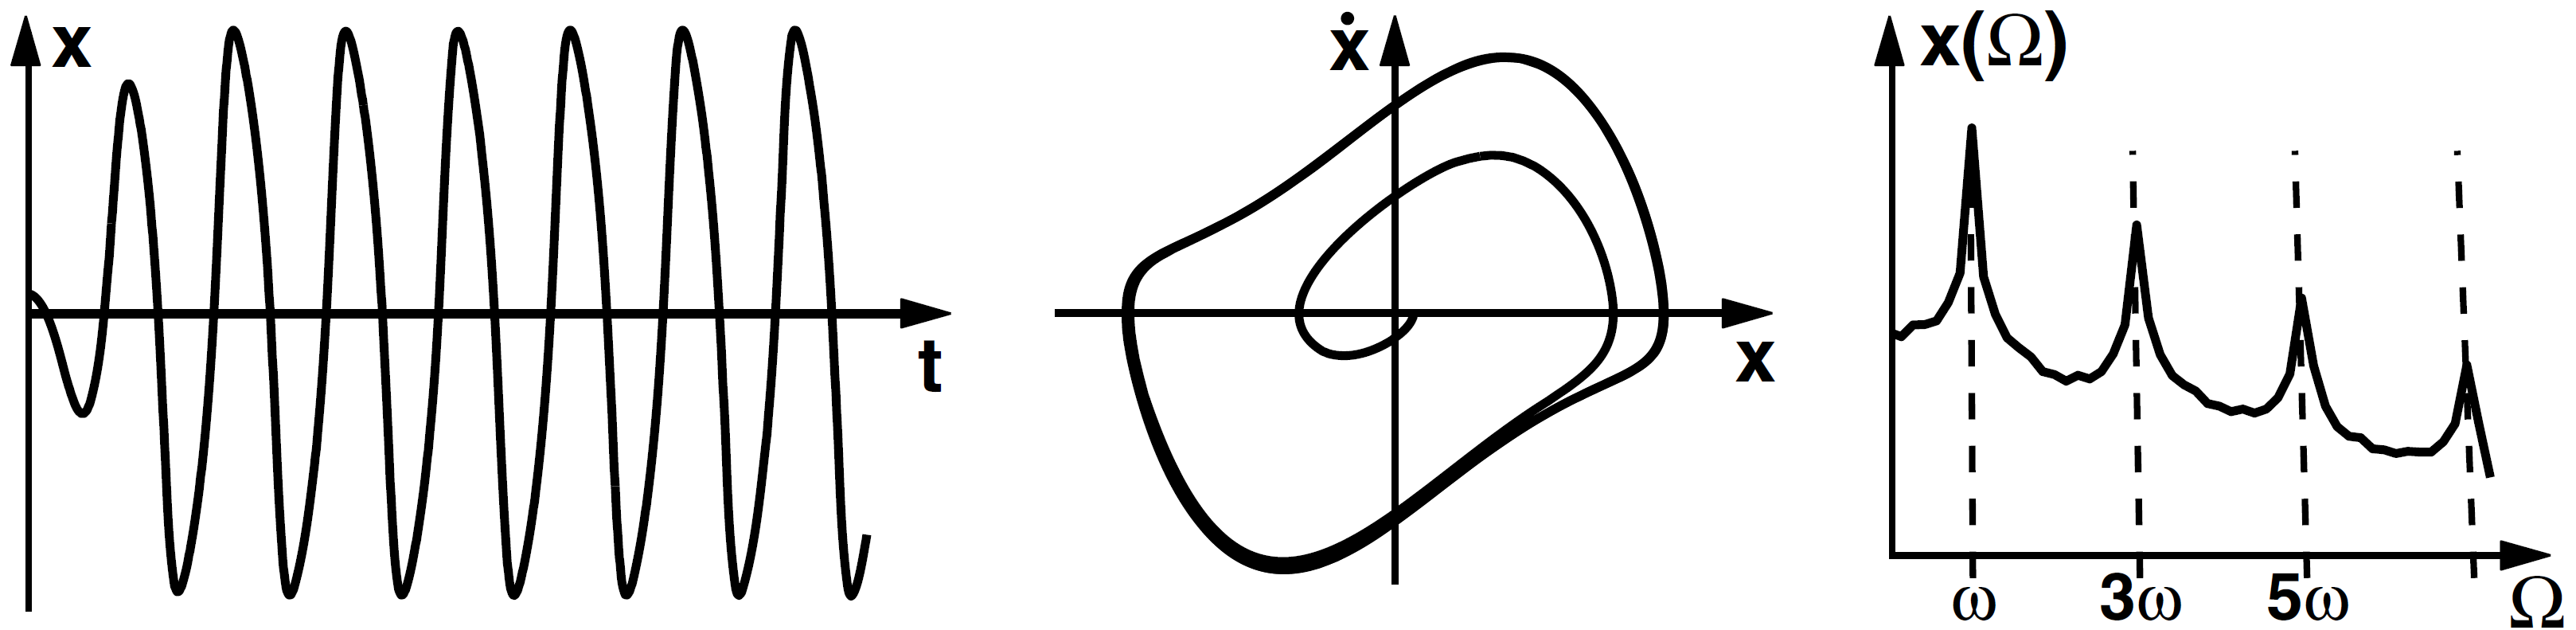
\includegraphics[width=\linewidth]{vdpo.png}
		\caption{The Van-der-Pol oscillator.}
		\label{fig:vdpo}
	\end{subfigure}
	\vline
	\begin{subfigure}{0.45\linewidth}
		\centering
		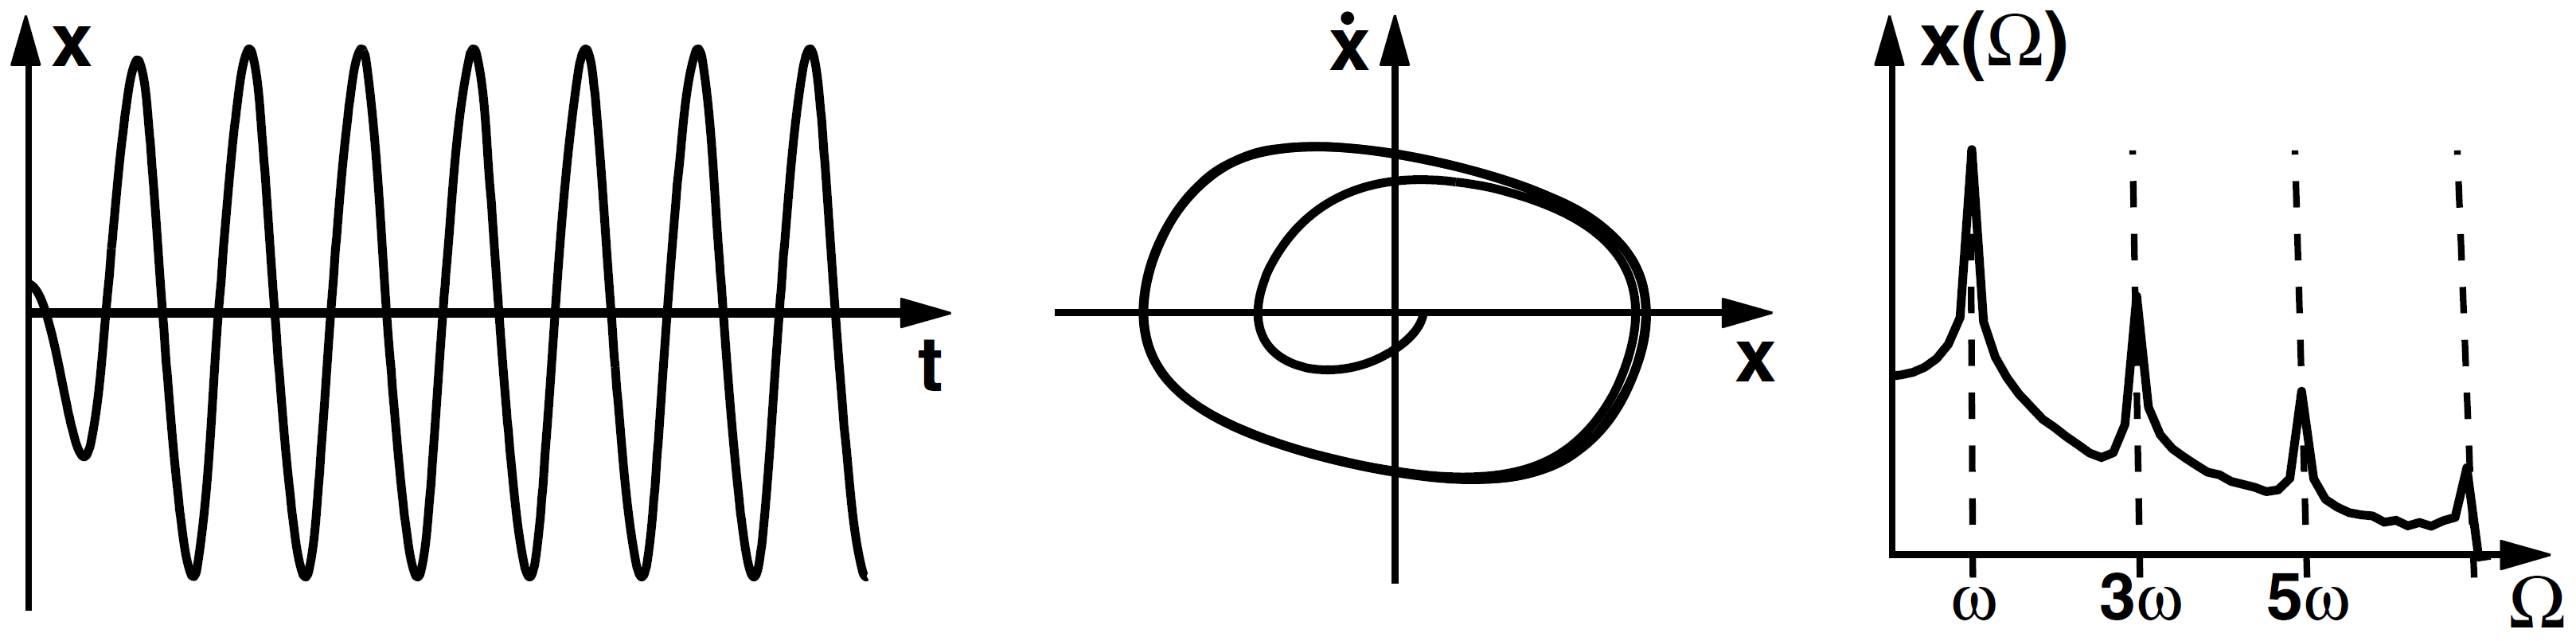
\includegraphics[width=\linewidth]{ro.png}
		\caption{The Rayleigh oscillator}
		\label{fig:ro}
	\end{subfigure}
	\caption{Time series (left), phase space trajectory (middle) and power spectrum (right).}
\end{figure}
\subsection{Rayleigh Oscillator: $N(x,\dot{x})=\dot{x}^3$}
The Rayleigh oscillator is given by
\begin{equation}{\label{eq:ro}}
	\ddot{x}+\gamma\dot{x}+\omega^2+\delta\dot{x}^3=0\quad\rightarrow\quad
	\ddot{x}+(\gamma+\delta\dot{x}^2)\dot{x}+\omega^2x=0
\end{equation}
The damping constant for the Rayleigh oscillator depends on the square of the velocity $\dot{x}^2$.
Arguments similar to those above lead to the conclusion that the Rayleigh oscillator shows sustained oscillations in the parameter range $\gamma<0$ and $\delta>0$.\\
As for the van-der-Pol oscillator, the phase space portrait is almost rectangular but rotated by about $90^\circ$.\\
It can be shown that for the van-der-Pol oscillator the amplitude is independent of frequency and for the Rayleigh it decreases proportional to $\omega^{-2}$.

\section{Bifurcations}{\label{sec:bf2d}}
If the phase portrait changes its topological structure (loses topological equivalence\footnote{Intuitively, two phase portraits are \emph{topologically equivalent} if one is a distorted version of the other. Bending and warping are allowed, but not ripping, so closed orbits must remain closed, trajectories connecting saddle points must not be broken, etc.}) as a parameter is varied, we say that a bifurcation has occurred.
\subsection{Codimension of a Bifurcation}
The codimension of a bifurcation is the \emph{number of parameters} which must be varied for the bifurcation to occur.
This corresponds to the codimension of the parameter set for which the bifurcation occurs within the full space of parameters.
\subsection{Local Bifurcations}{\label{sec:lb}}
A \emph{local} bifurcation occurs when a parameter change causes the stability of an equilibrium (or fixed point) to change.
In continuous systems, this corresponds to the real part of an eigenvalue of an equilibrium passing through zero.
In discrete systems (those described by maps rather than ODEs) (See Section (\ref{sec:dds})), this corresponds to a fixed point having a \emph{Floquet multiplier} with modulus equal to one.
In both cases, the equilibrium is \emph{non-hyperbolic} at the bifurcation point.
The topological changes in the phase portrait of the system can be confined to arbitrarily small neighbourhoods of the bifurcating fixed points by moving the bifurcation parameter close to the bifurcation point (hence \emph{local}).\\\\
\textbullet\quad\textbf{Bifurcations at $\lambda_1=0$ or $\lambda_2=0$}
\subsubsection{Saddle-Node Bifurcation}{\label{sec:snbf2}}
The prototypical example in two dimensions is given by
\begin{equation}
	\begin{aligned}
		\dot{x}&=\mu-x^2\\
		\dot{y}&=-y
	\end{aligned}
\end{equation}
Consider the phase portrait as $\mu$ varies.
For $\mu=0$, Figure (\ref{fig:snbf2}) shows that there are two fixed points, a stable node at $(\tilde{x},\tilde{y})=(\sqrt{\mu},0)$ and a saddle at $(-\sqrt{\mu},0)$.
\begin{figure}[h!]
	\centering
	\begin{subfigure}{0.45\linewidth}
		\centering
		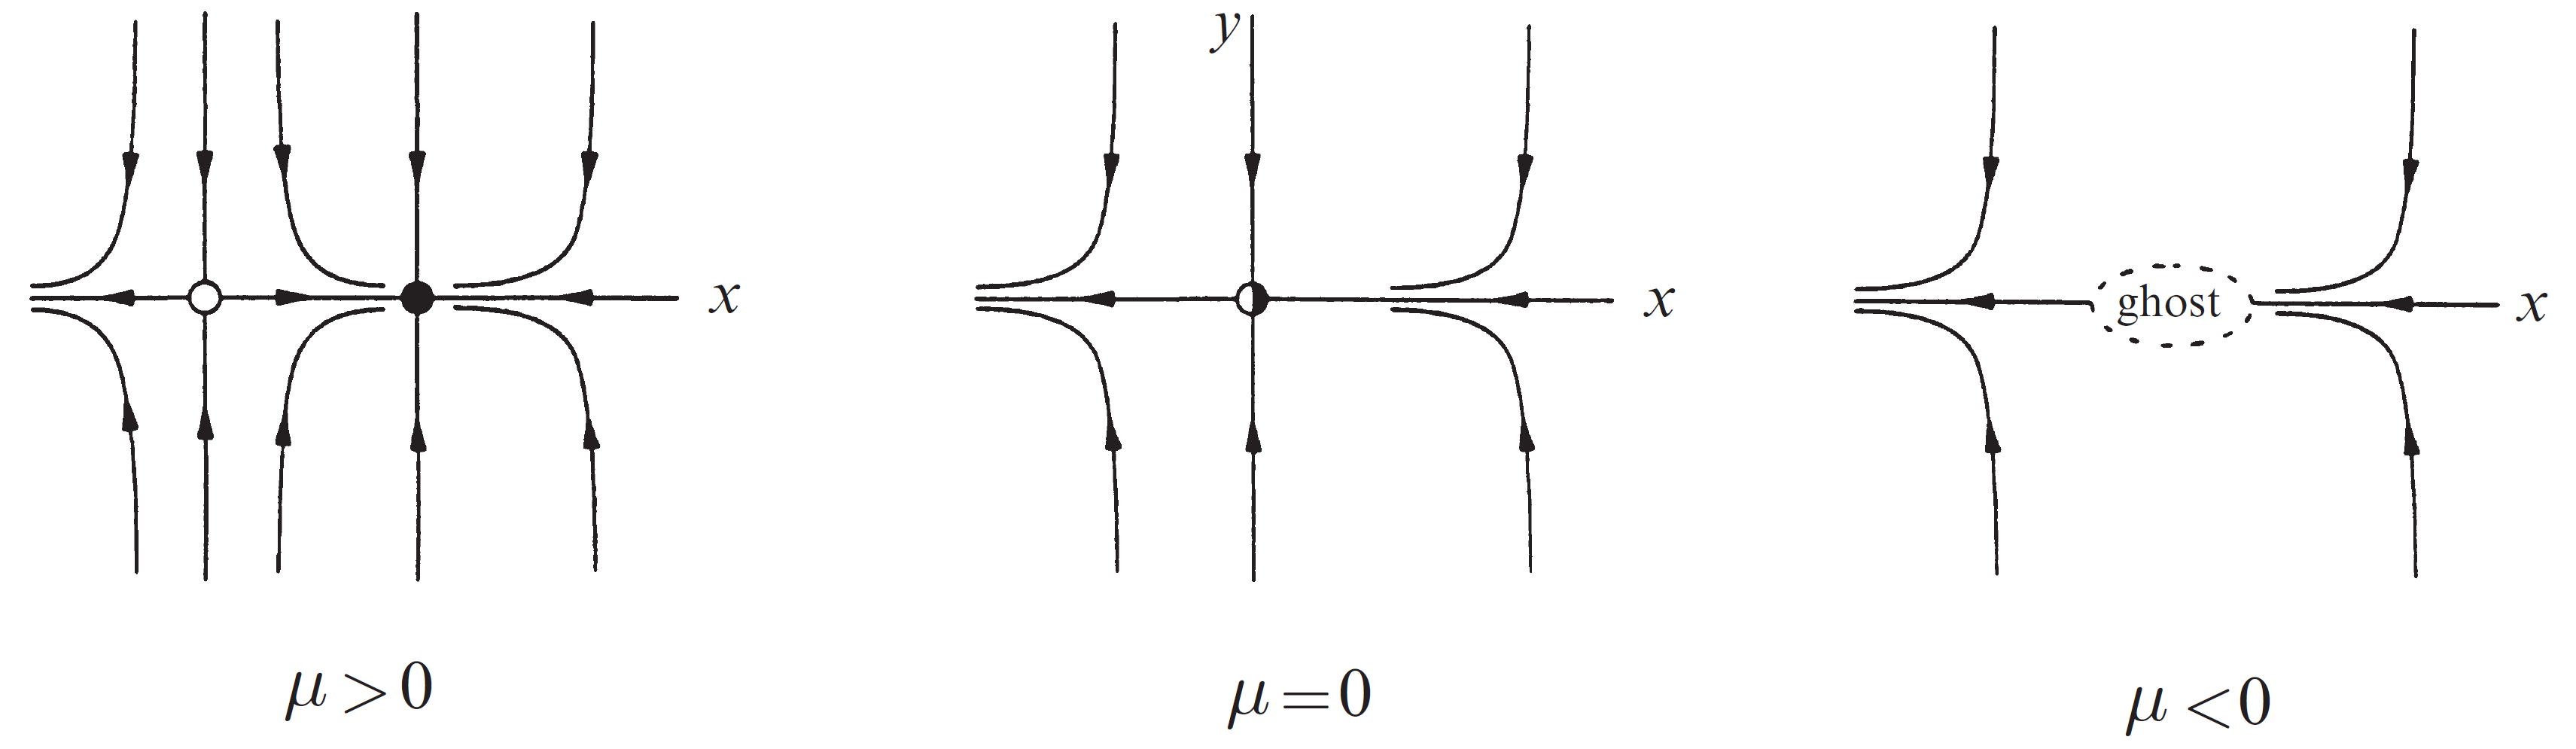
\includegraphics[width=\linewidth]{snbf2.png}
		\caption{Saddle-Node Bifurcation}
		\label{fig:snbf2}
	\end{subfigure}
	\vline
	\begin{subfigure}{0.42\linewidth}
		\centering
		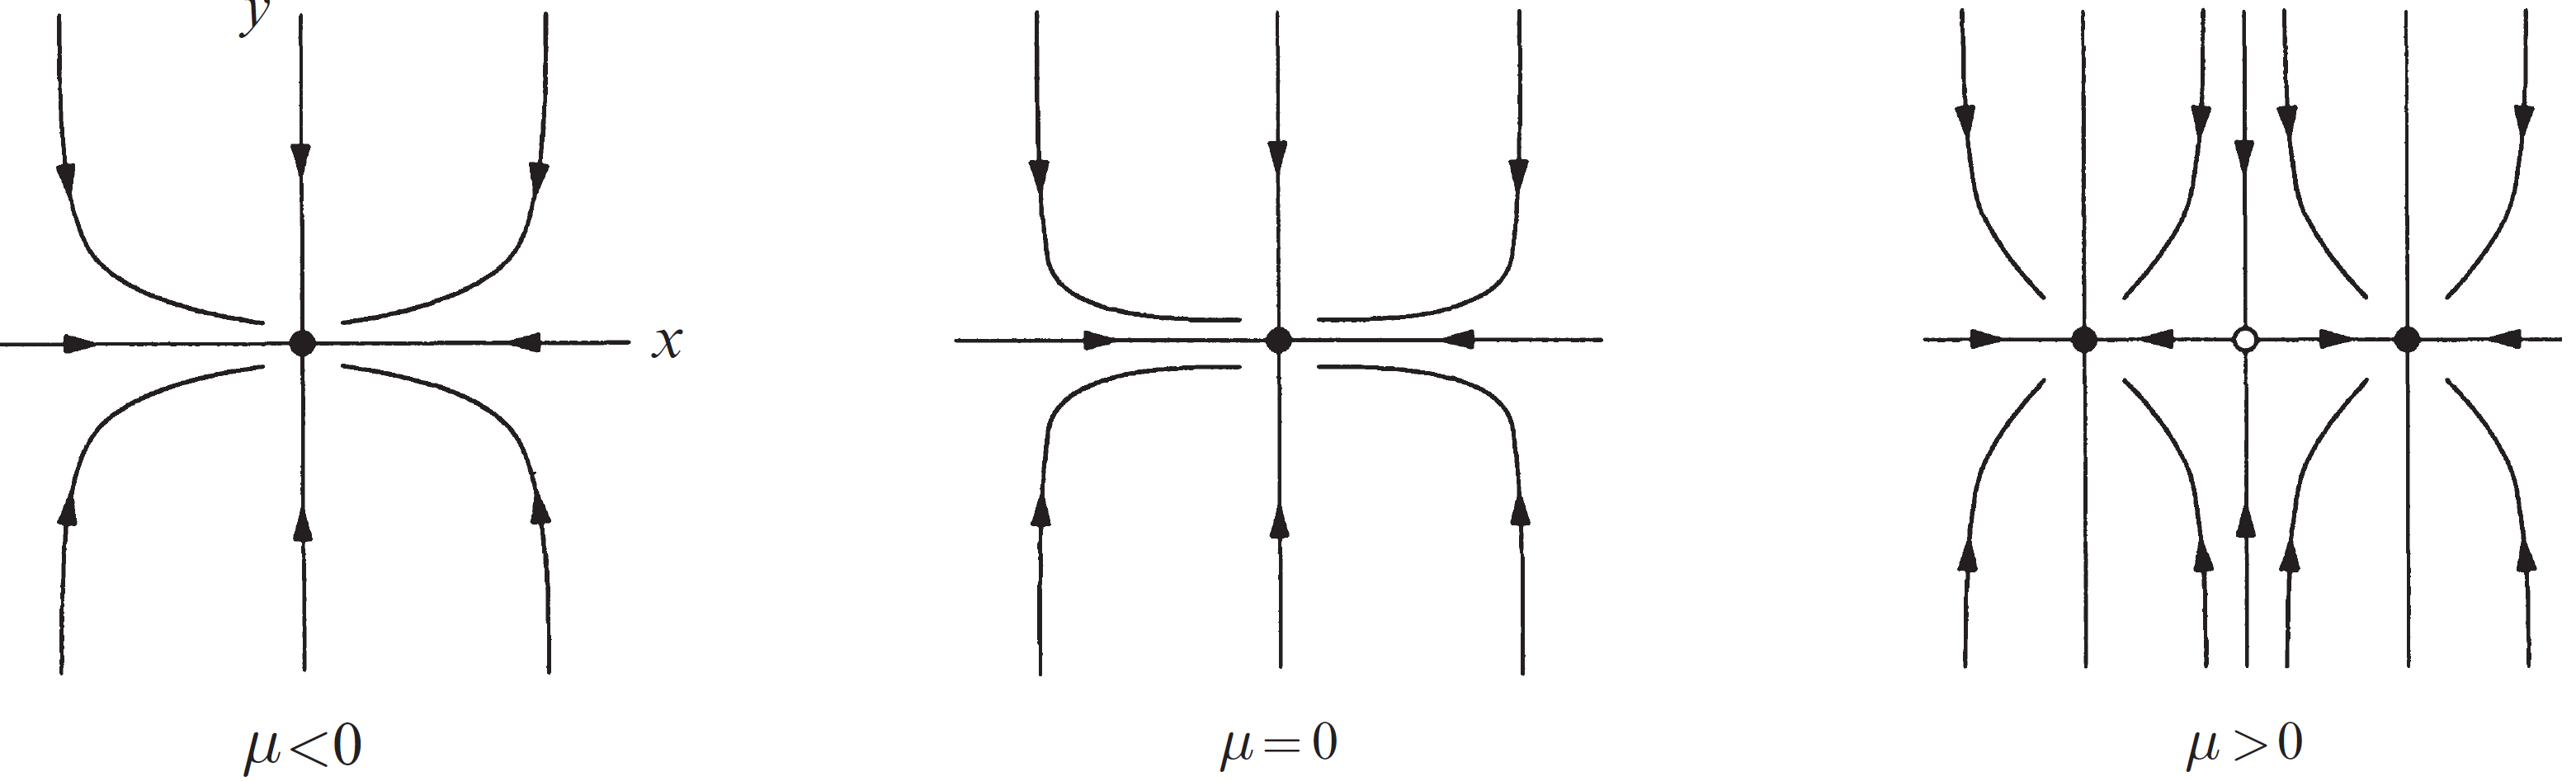
\includegraphics[width=\linewidth]{spbf2.png}
		\caption{Supercritical Pitchfork Bifurcation}
		\label{fig:spbf2}
	\end{subfigure}
	\caption{}
\end{figure}
As $\mu$ decreases, the saddle and node approach each other, then collide when $\mu=0$ and finally disappear when $\mu<0$.
Even after the fixed points have annihilated each other, they continue to influence the flow as in Section (\ref{sec:nuo}), they leave a \emph{ghost}, a bottleneck region that sucks trajectories in and delays them before allowing passage out the other side.
\subsubsection{Transcritical Bifurcation}
The prototypical example in two dimensions is given by
\begin{equation}
\begin{aligned}
\dot{x}&=\mu x-x^2\\
\dot{y}&=-y
\end{aligned}
\end{equation}
This system has always two distinct fixed points $(0,0)$ and $(\mu,0)$ for $\mu\neq0$. For $\mu=0$, these two fixed points merge at $(0, 0)$.
\begin{comment}
	\begin{figure}[h!]
	\centering
	\begin{subfigure}{0.45\linewidth}
	\centering
	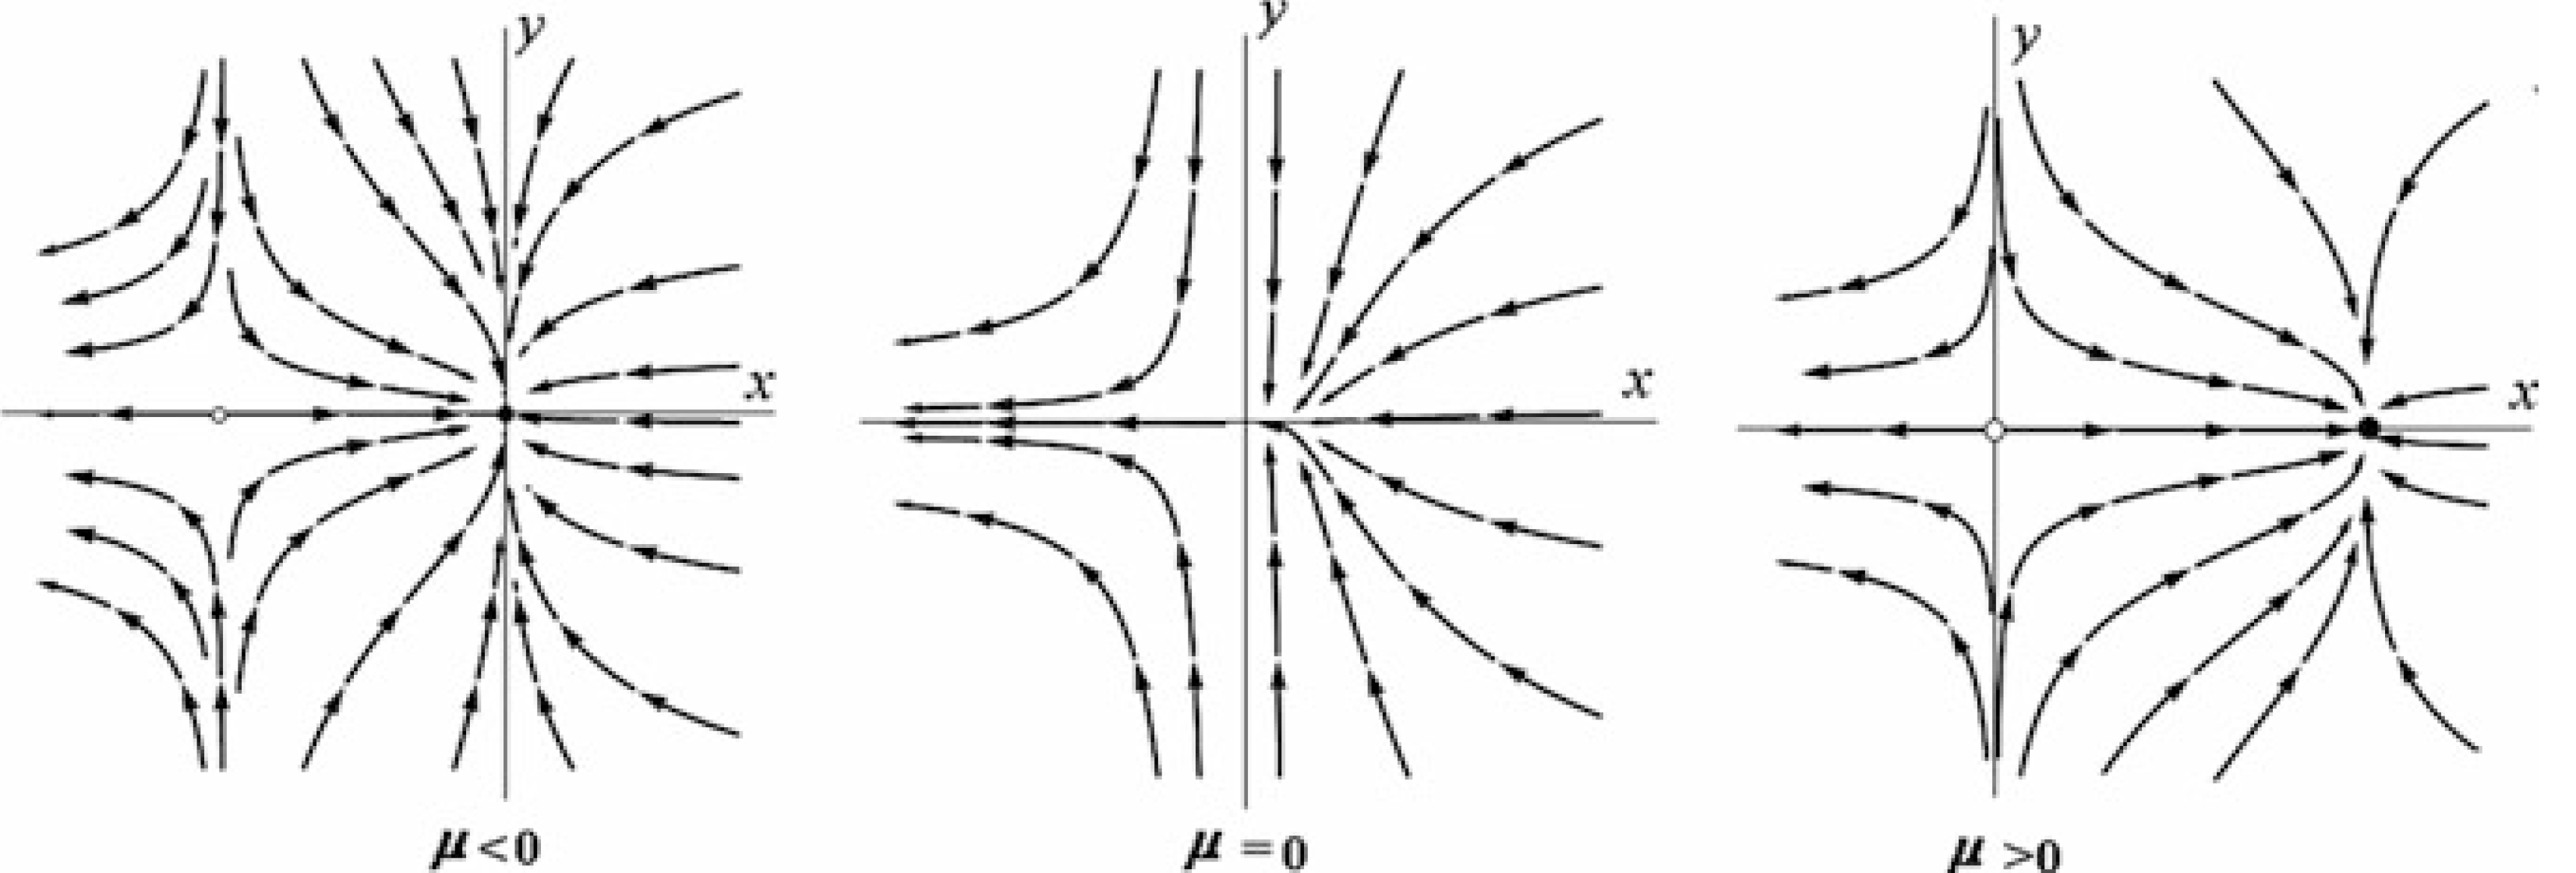
\includegraphics[width=\linewidth]{tbf2.png}
	\caption{Transcritical Bifurcation}
	\label{fig:tbf2}
	\end{subfigure}
	\vline
	\begin{subfigure}{0.45\linewidth}
	\centering
	\includegraphics[width=\linewidth]{sbbf2.png}
	\caption{Subcritical Pitchfork Bifurcation}
	\label{fig:sbbf2}
	\end{subfigure}
	\caption{}
	\end{figure}
\end{comment}
From the Phase portrait, we see that the behavior of the system changes when the parameter $\mu$ passes through the origin.
When $\mu$ passes through the origin from left, the fixed point origin changes to a saddle from a stable node and the fixed point $(\mu,0)$ changes from a saddle to a stable node.
\subsubsection{Supercritical Pitchfork Bifurcation}
The prototypical example in two dimensions is given by
\begin{equation}
	\begin{aligned}
		\dot{x}&=\mu x-x^3\\
		\dot{y}&=-y
	\end{aligned}
\end{equation}
For $\mu<0$, the only fixed point is a stable node at the origin. For $\mu=0$, the origin is still stable, but now we have very slow (algebraic) decay along the x-direction instead of exponential decay.
For $\mu>0$, the origin loses stability (becomes a saddle) and gives birth to two new stable fixed points symmetrically located at $(\pm\sqrt{\mu},0)$
\subsubsection{Subcritical Pitchfork Bifurcation}
The prototypical example in two dimensions is given by
\begin{equation}
	\begin{aligned}
		\dot{x}&=\mu x+x^3\\
		\dot{y}&=-y
	\end{aligned}
\end{equation}
\textbullet\quad\textbf{Hopf Bifurcations at $\lambda_{1,2}=\pm i\omega$}
\subsubsection{Supercritical Hopf bifurcation}
We consider the dynamical system
\begin{equation}{\label{eq:sphb}}
	\dot{\xi}=\mu\ \xi-\xi\ |\xi|^2\quad\text{with}\quad\mu,\xi\in\mathbb{C}\quad\text{Let}\quad
	\begin{cases}
		\mu=\epsilon+i\omega\\
		\xi=x+iy
	\end{cases}
\end{equation}
We see that (\ref{eq:sphb}) is indeed a two-dimensional dynamical system
\begin{equation}
	\begin{aligned}
		\dot{x}&=\epsilon x-\omega y-x(x^2+y^2)\\
		\dot{y}&=\omega x+\epsilon y-y(x^2+y^2)
	\end{aligned}\quad\rightarrow\quad
	\begin{aligned}
		\dot{r}&=\epsilon r-r^3\\
		\dot{\varphi}&=\omega
	\end{aligned}
\end{equation}
\begin{wrapfigure}{r}{0.4\linewidth}
	\centering
	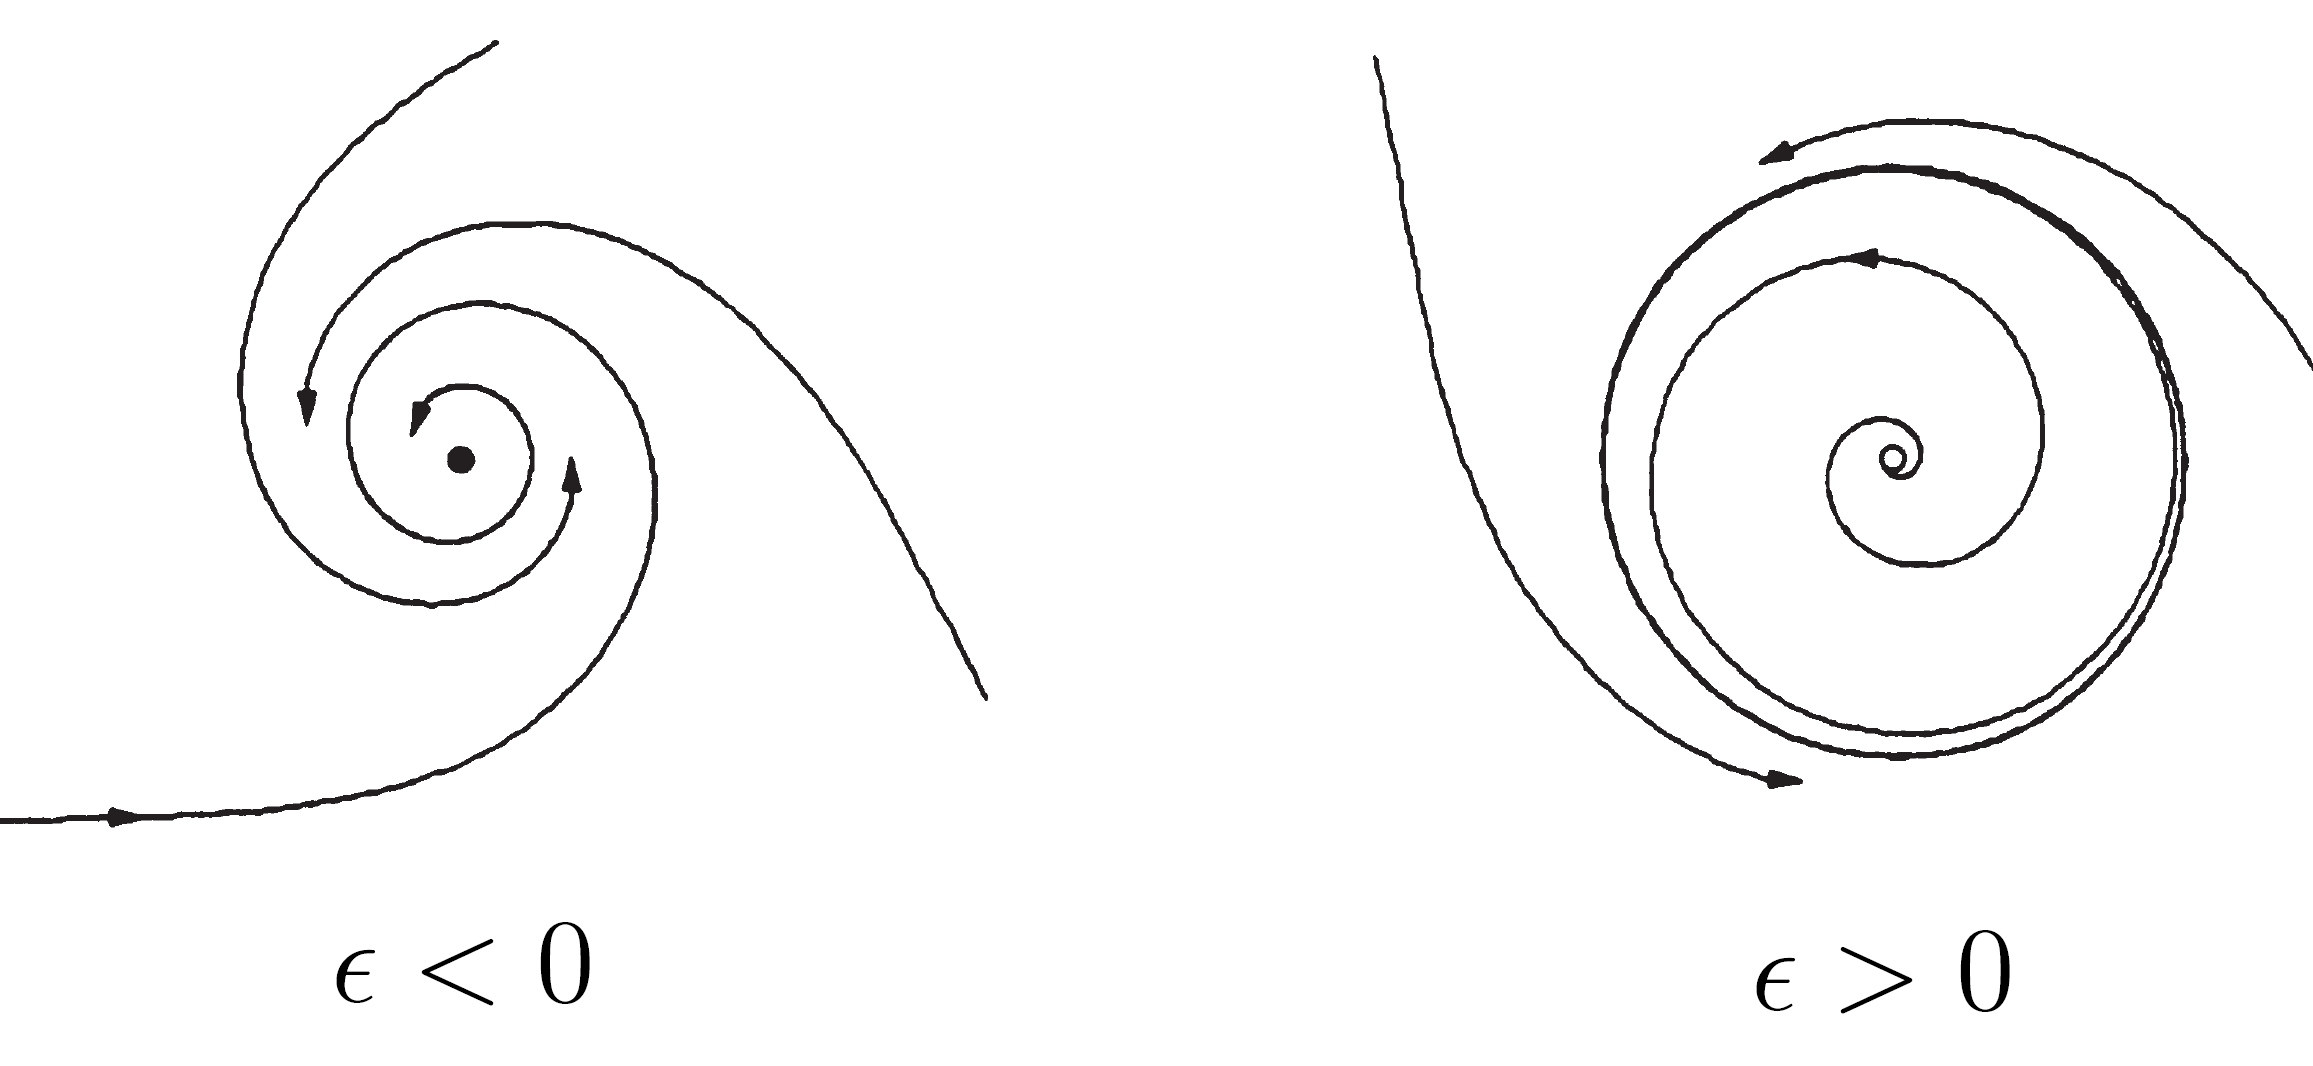
\includegraphics[width=\linewidth]{sphbf.png}
	\caption{Supercritical Hopf bifurcation}
	\label{fig:sphbf}
\end{wrapfigure}
As we have seen earlier (Equation (\ref{eq:spbf})), this equation has a single stable fixed point $r=0$ for $\epsilon<0$ and undergoes a supercritical pitchfork bifurcation at $\epsilon=0$, which turns this fixed point unstable and gives rise to two new stable fixed points at $r=\pm\sqrt{\epsilon}$.
Interpreting $r$ as the radius of a limit cycle, we find that a stable limit cycle with radius $\sqrt{\epsilon}$ arises from a fixed point when $\epsilon$ exceeds its critical value $\epsilon=0$.
\begin{equation}{\label{eq:sphbf}}
	\begin{pmatrix}
		\dot{x}\\\dot{y}
	\end{pmatrix}=
	\begin{pmatrix}
		\epsilon&-\omega\\
		\omega&\epsilon
	\end{pmatrix}=
	\begin{pmatrix}
		x\\y
	\end{pmatrix}
\end{equation}
The eigenvalues $\lambda$ for the matrix in (\ref{eq:sphbf}) are
\begin{equation}
	\lambda_{1,2}=\epsilon\pm i\omega
\end{equation}
\begin{comment}
	\begin{figure}[h!]
	\centering
	\begin{subfigure}{0.45\linewidth}
	\centering
	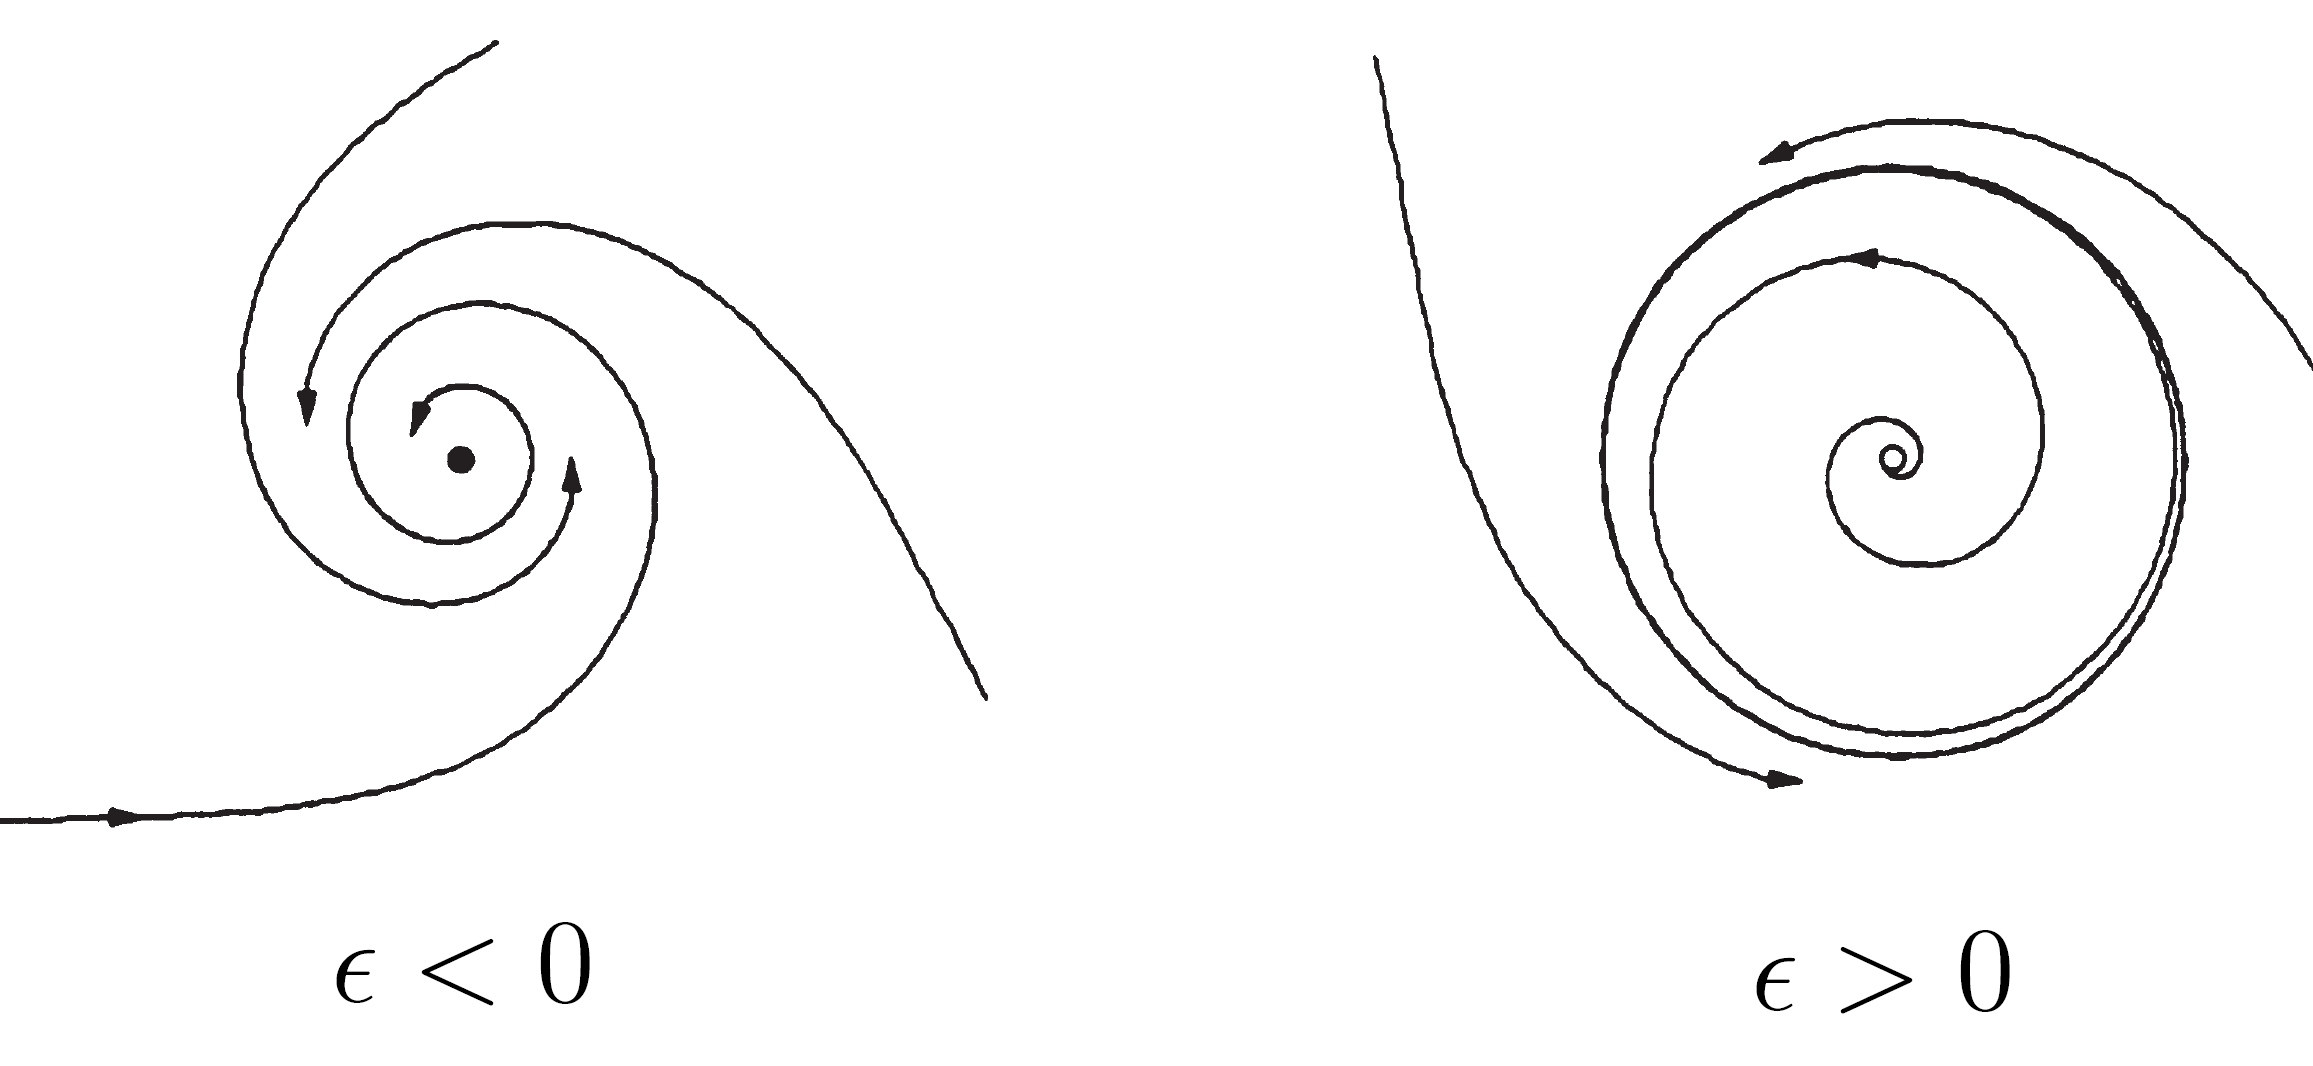
\includegraphics[width=\linewidth]{sphbf.png}
	\caption{Supercritical Hopf bifurcation}
	\label{fig:sphbf}
	\end{subfigure}
	\vline
	\begin{subfigure}{0.354\linewidth}
	\centering
	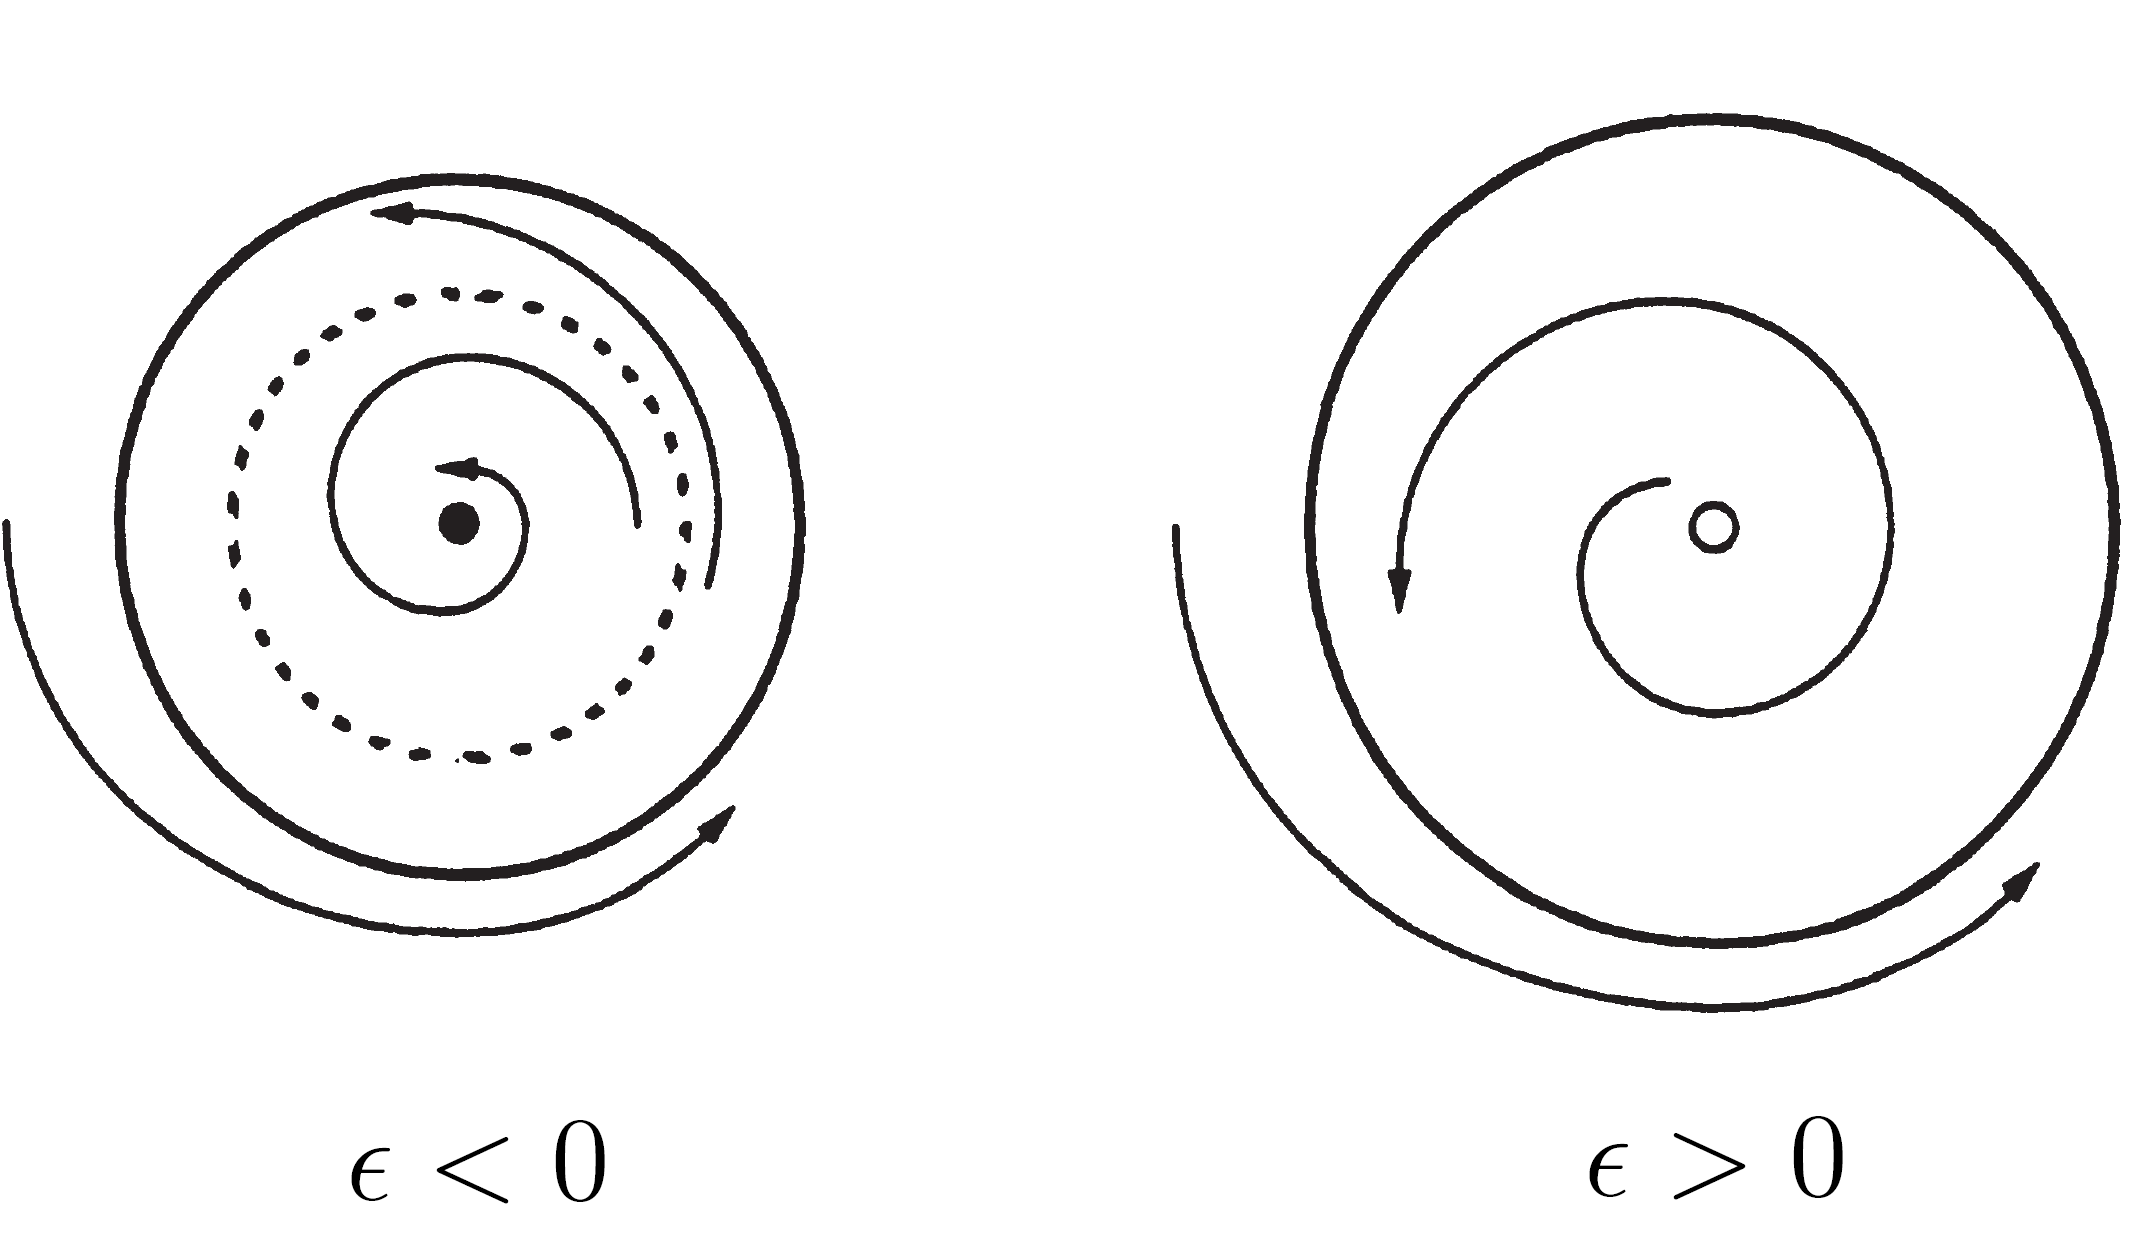
\includegraphics[width=\linewidth]{sbhbf.png}
	\caption{Subcritical Hopf bifurcation}
	\label{fig:sbhbf}
	\end{subfigure}
	\end{figure}
\end{comment}
A Supercritical Hopf bifurcation occurs when a stable spiral changes into an unstable spiral surrounded by a small, nearly elliptical limit cycle (Figure (\ref{fig:sphbf})).
\subsubsection{Subcritical Hopf Bifurcation}
Consider
\begin{equation}{\label{eq:sbhbf}}
	\begin{aligned}
		\dot{r}&=\epsilon r+2r^3-r^5\\
		\dot{\varphi}&=\omega
	\end{aligned}
\end{equation}
The fixed points are given by
\begin{equation}
	\tilde{r}_1=0\quad\tilde{r}_{2,3}^2=1\pm\sqrt{1+\epsilon}
\end{equation}
\begin{figure}[h!]
	\centering
	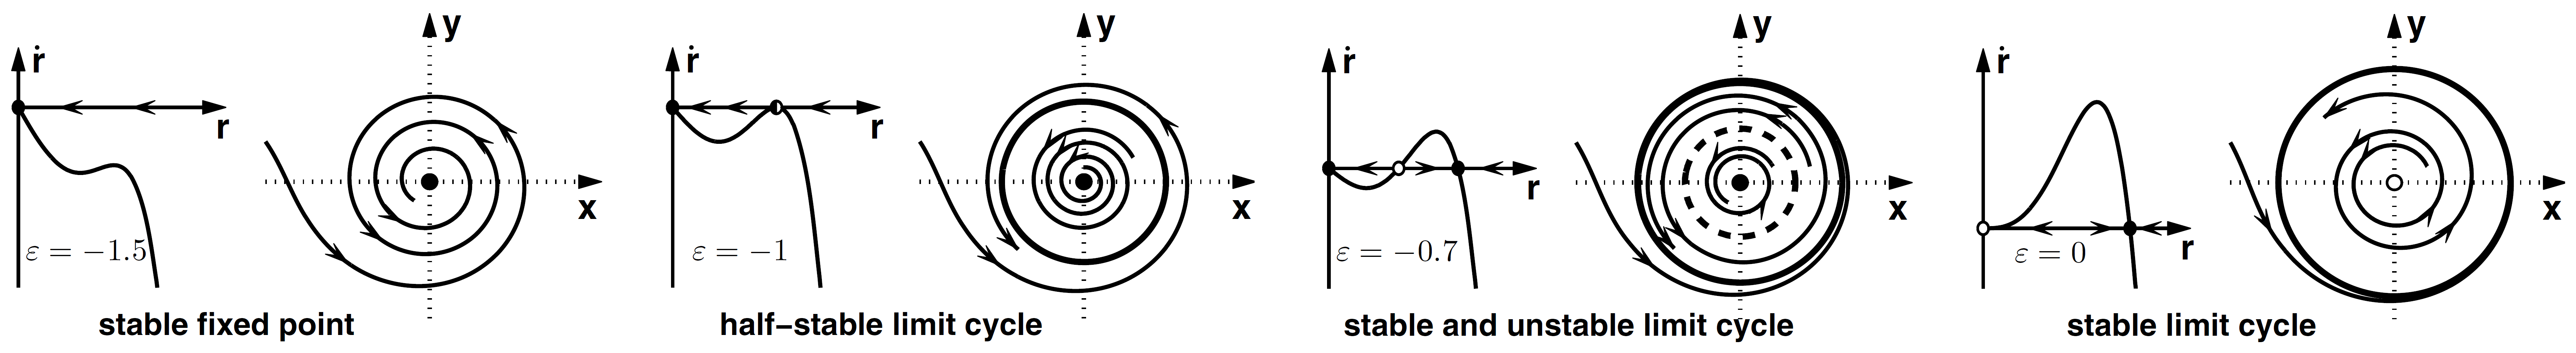
\includegraphics[width=\linewidth]{sbhbf2.png}
	\caption{Bifurcation sequence for the subcritical Hopf bifurcation.}
	\label{fig:sbhbf}
\end{figure}
For $\epsilon<-1$ (top left) $r_1=0$ is the only real solution of (\ref{eq:sbhbf}) and all trajectories spiral towards the origin, which is a stable fixed point.
At $\epsilon=-1$ (top right) a half-stable limit cycle exists where trajectories from the outside are attracted onto it and trajectories on the inside are repelled and evolve towards the origin.
For $-1<\epsilon<0$ the phase space plot in Figure (\ref{fig:sbhbf}) (bottom left) contains a stable fixed point at the origin and two limit cycles.
The inner limit cycle with a radius $r=\sqrt{1-\sqrt{1+\epsilon}}$ is unstable with trajectories moving away towards the still stable fixed point at the origin and a stable limit cycle with $r=\sqrt{1+\sqrt{1+\epsilon}}$.
At $\epsilon=0$ the unstable limit cycle and the stable fixed point at the origin collide, leaving a system with a single stable orbit with radius $r=\sqrt{2}$ and an unstable fixed point at the origin as shown in Figure (\ref{fig:sbhbf}) (bottom right).
\subsection{Global Bifurcations}
Global bifurcations occur when \emph{larger invariant sets}, such as \emph{periodic orbits}, collide with equilibria.
This causes changes in the topology of the trajectories in the phase space which cannot be confined to a small neighbourhood, as is the case with local bifurcations.
In fact, the changes in topology extend out to an arbitrarily large distance (hence \emph{global}).
\subsubsection{Infinite-Period Bifurcation}
Consider the system
\begin{equation}
	\begin{aligned}
		\dot{r}&=r(1-r^2)\\
		\dot{\theta}&=\mu-\sin\theta
	\end{aligned}
	\quad\text{where}\quad\mu\geq0
\end{equation}
In the radial direction, all trajectories (except $\tilde{r}=0$) approach the unit circle monotonically as $t\rightarrow\infty$.
In the angular direction, the motion is everywhere counterclockwise if $\mu>1$, whereas there are two invariant rays defined by $\sin\theta=\mu$ if $\mu<1$. As $\mu$ decreases, the limit cycle $r=1$ develops a bottleneck at $\theta=\pi/2$ that becomes increasingly severe as $\mu\rightarrow1^+$.
The oscillation period lengthens and finally becomes infinite at $\mu_c=1$, when a fixed point appears on the circle; hence the term \emph{infinite-period bifurcation}.
For $\mu<1$, the fixed point splits into a saddle and a node.
\begin{figure}[h!]
	\centering
	\begin{subfigure}{0.27\linewidth}
		\centering
		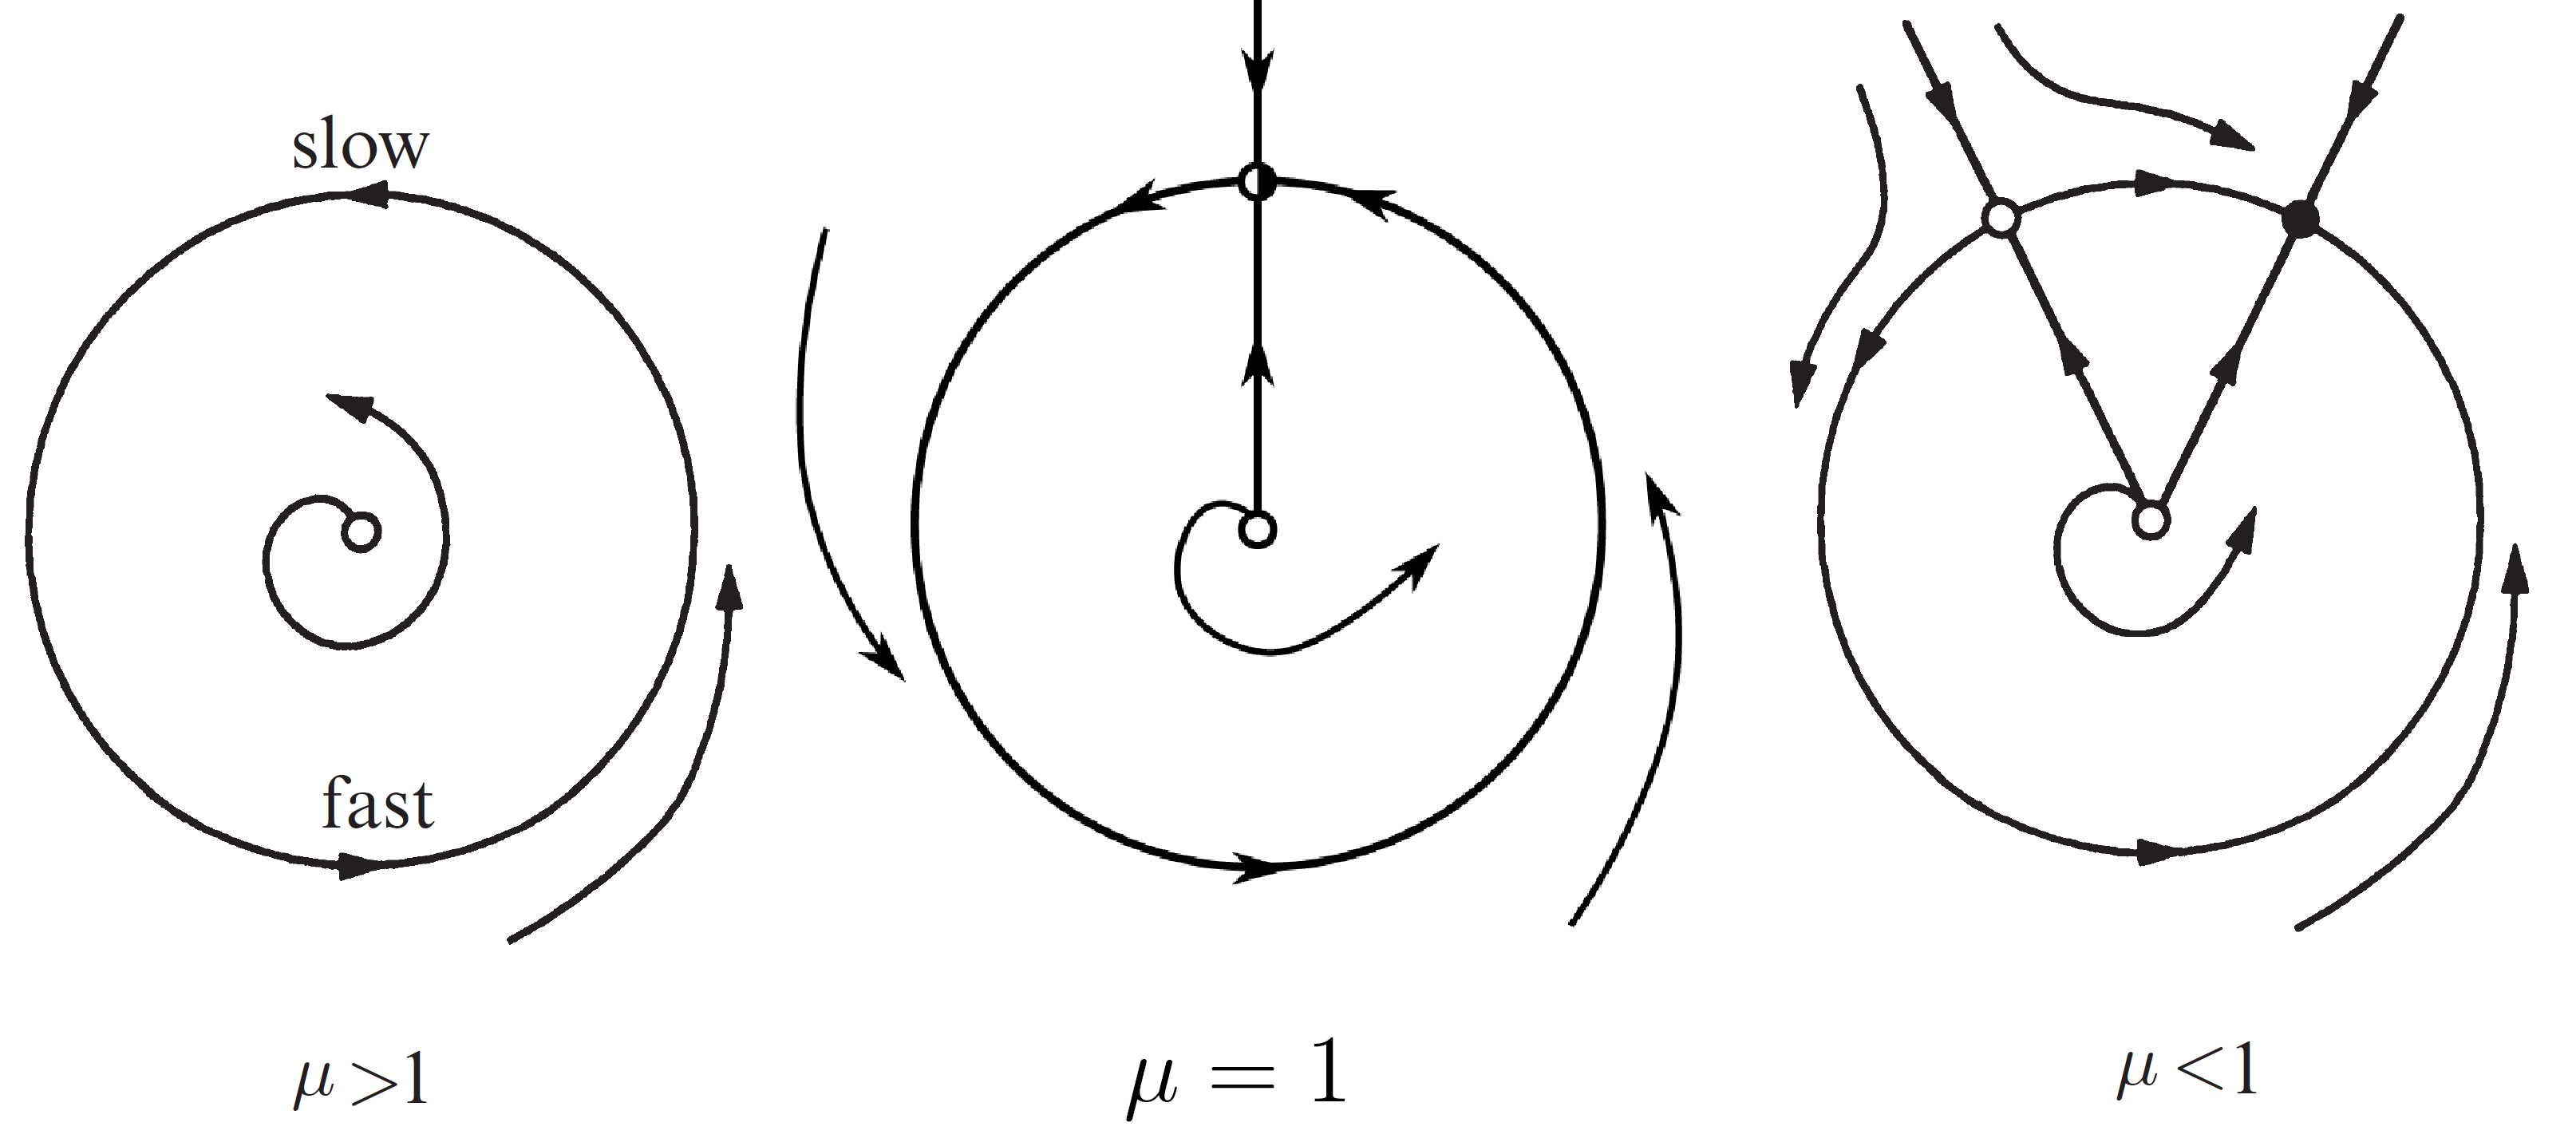
\includegraphics[width=\linewidth]{ipbf.png}
		\caption{Infinite-Period\\Bifurcation}
		\label{fig:ipbf}
	\end{subfigure}
	\vline
	\begin{subfigure}{0.7\linewidth}
		\centering
		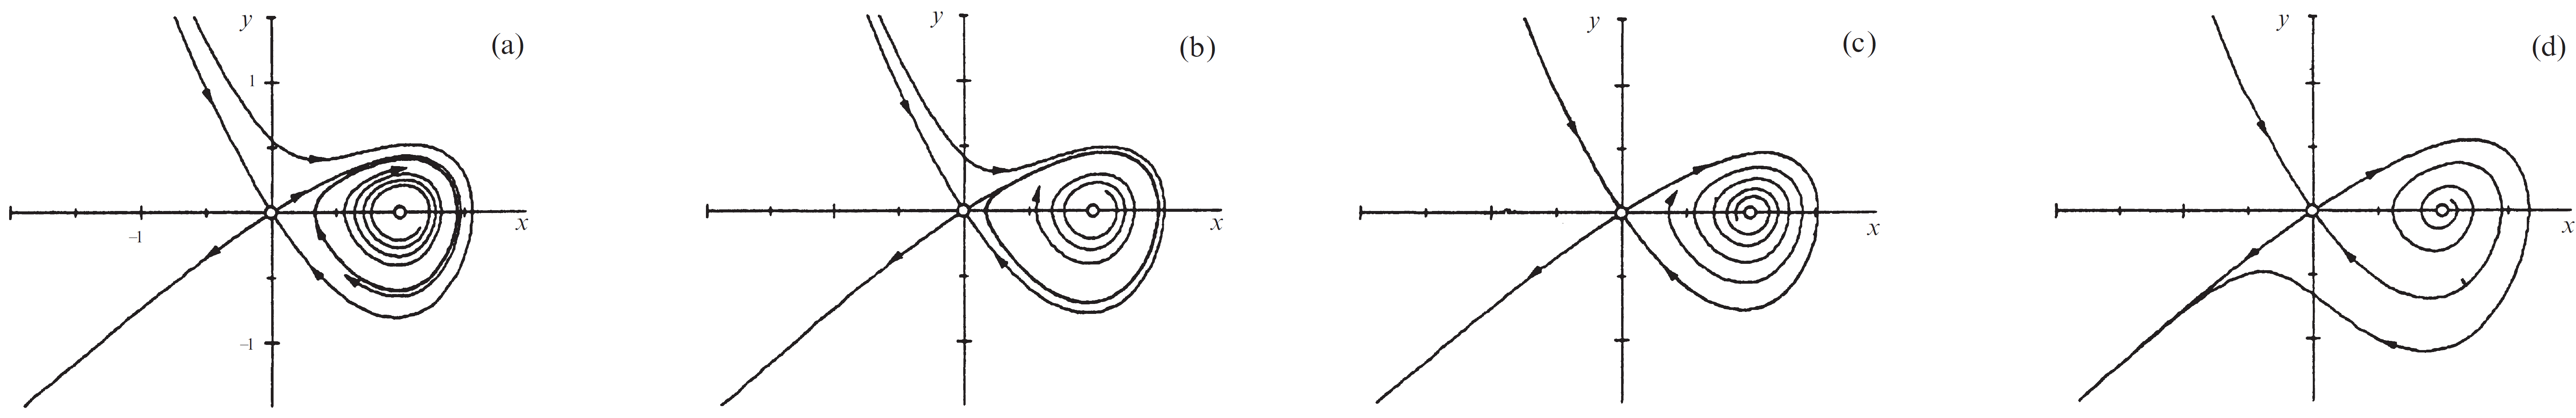
\includegraphics[width=\linewidth]{hcbf.png}
		\caption{Homoclinic Bifurcation}
		\label{fig:hcbf}
	\end{subfigure}
	\caption{}
\end{figure}
\subsubsection{Homoclinic Bifurcation}
Consider the system
\begin{equation}
	\begin{aligned}
		\dot{x}&=y\\
		\dot{y}&=\mu y+x-x^2+xy
	\end{aligned}
\end{equation}
Numerically, the bifurcation is found to occur at $\mu_c\approx-0.8645$. For $\mu<\mu_c$, say $\mu=-0.92$, a stable limit cycle passes close to a saddle point at the origin (Figure (\ref{fig:hcbf}a)).
As $\mu$ increases to $\mu_c$, the limit cycle swells (Figure (\ref{fig:hcbf}b)) and bangs into the saddle, creating a homoclinic orbit (Figure (\ref{fig:hcbf}c)).
Once $\mu>\mu_c$, the saddle connection breaks and the loop is destroyed (Figure (\ref{fig:hcbf}d)).
\subsubsection{Heteroclinic Bifurcation}
Here, a limit cycle collides with two or more saddle points.\\
This type of bifurcation will result in the change of stability of the heteroclinic cycle.
\paragraph{Resonance Bifurcations}
The stability of the cycle changes when an algebraic condition on the eigenvalues of the equilibria in the cycle is satisfied.
This is usually accompanied by the \emph{birth} or \emph{death} of a \emph{periodic orbit}.
\paragraph{Transverse Bifurcation}
It is caused when the real part of a transverse eigenvalue of one of the equilibria in the cycle passes through zero.
\subsubsection{Crisis}
A \textbf{crisis} is the sudden appearance or disappearance of a strange attractor as the parameters of a dynamical system are varied.
It occurs when a chaotic attractor comes into contact with an unstable periodic orbit or its stable manifold.
\paragraph{Exterior Crisis}
The attractor is suddenly \emph{destroyed} as the parameters are varied.
In the postbifurcation state the motion is transiently chaotic, moving chaotically along the former attractor before being attracted to a fixed point, periodic orbit, quasiperiodic orbit, another strange attractor, or diverging to infinity.
\paragraph{Interior Crisis}
The \emph{size} of the chaotic attractor suddenly \emph{increases}.
The attractor encounters an unstable fixed point or periodic solution that is inside the basin of attraction.
\paragraph{Attractor Merging Crisis}
Two or more chaotic attractors \emph{merge} to form a single attractor as the critical parameter value is passed.

\newpage
\part{Higher Dimensional Systems}
The existence and uniqueness theorem (\ref{thm:eut}) holds.\\
Linear Stability Analysis and Potential Functions both generalize from lower dimensional analogues.
\begin{theorem}
	Consider the differential equation
	\begin{equation*}
		\mathbf{\dot{x}}=\mathbf{f}(\mathbf{x})\quad\mathbf{x}\in\mathbb{R}^n
	\end{equation*}
	Suppose that $\mathbf{f}(\mathbf{0})=\mathbf{0}$ and that the Jacobian matrix has $n$ eigenvalues with nonzero real part.
	Then, in a small neighborhood of $\mathbf{x}=0$, there exist stable and unstable manifolds with the \emph{same dimensions} as the stable and unstable manifolds of the linearized system
	\begin{equation*}
		\mathbf{\dot{x}}=J\mathbf{x}
	\end{equation*}
\end{theorem}

\section{Three Dimensional Systems}
\subsection{Periodicity and Quasi-periodicity}{\label{sec:paqp}}
By increasing the dimension of a system from one to two, we found a new type of attractor: the limit cycle.
Similarly, new things emerge in higher dimensions.\\
Consider a trajectory given by the superposition of a movement along a circle inside the torus and a circle around the torus as shown at the top left.
Each of these circles has a corresponding frequency, say $\omega_i$ being the frequency for the inside circle and $\omega_a$ for the one that goes around.
As long as the ratio between $\omega_i$ and $\omega_a$ is a rational number the trajectories are closed after a finite number of turns inside and around the torus: the flow is {\textbf{periodic}}.
Such a closed trajectory represents a limit cycle in three dimensions.
When the ratio between the two frequencies is an irrational number, the trajectory never closes and, as time evolves, covers the torus more and more densely.
Such dynamics are called {\textbf{quasi-periodic}}.
\begin{figure}[h!]
	\centering
	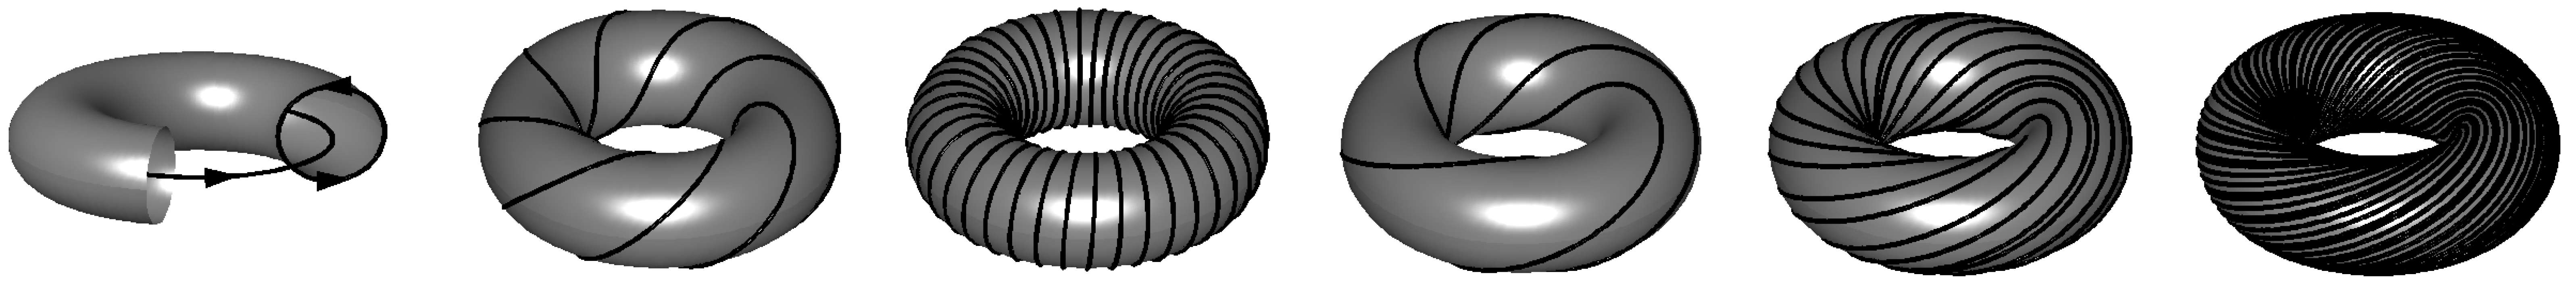
\includegraphics[width=\linewidth]{paqp.png}
	\caption{a) Flow on the surface of a torus can be described by a superposition of movements along two circles, one inside the torus and one around it.\\b) Here $\omega_i:\omega_a=8:3$.\\c) Here $\omega_i:\omega_a=1:40$.\\d) e) f) Here $\omega_i:\omega_a=\sqrt{2}$.}
	\label{fig:paqp}
\end{figure}
\subsection{Lorenz System}{\label{sec:ls}}
\paragraph{The Lorenz Equations}
In 1963, the MIT meteorologist Edward Lorenz constructed a highly simplified model of a convecting fluid.
This simple model also displays a wide variety of behavior and for some parameter values is chaotic.
\begin{equation}{\label{eq:ls}}
	\begin{aligned}
		\dot{x}&=\sigma(y-x)\\
		\dot{y}&=rx-y-xz\quad\text{with}\quad r,b,\sigma\geq0\\
		\dot{z}&=xy-bz
	\end{aligned}
\end{equation}
here $x$ measures the rate of convective overturning, $y$ measures the horizontal temperature variation, $z$ measures the vertical temperature variation, $\sigma$ is the \emph{Prandtl number}, $r$ is the \emph{Rayleigh number}, and $b$ is a scaling factor.
The Prandtl number is related to the fluid viscosity, and the Rayleigh number is related to the temperature difference between the top and bottom of the column.
Lorenz studied the system when $\sigma=10$ and $b=\frac{8}{3}$.\\
\subsubsection{Properties of Lorenz System}
\begin{itemize}
	\item System (\ref{eq:ls}) has natural symmetry $(x, y, z)\rightarrow(-x,-y, z)$.
	\item The $z-$axis is invariant.
	\item The flow is volume contracting since $\nabla\cdot\mathbf{x}=-(\sigma+b+1)<0$, where $\mathbf{x}$ is the vector field.
	\item The Lorenz system (\ref{eq:ls}) has the fixed points
	\begin{equation}{\label{eq:sls}}
		\mathbf{\tilde{x}}_1=
		\begin{pmatrix}
			0\\0\\0
		\end{pmatrix}\quad\text{and}\quad
		\mathbf{\tilde{x}}_{2,3}=
		\begin{pmatrix}
			\pm\sqrt{b(r-1)}\\[5pt]
			\pm\sqrt{b(r-1)}\\[5pt]
			r-1
		\end{pmatrix}\quad\text{if}\quad r\geq1
	\end{equation}
	As before, the stability of the fixed points is determined by the Jacobian matrix $J(x)$, which is given explicitly for the general three-dimensional case and $J_L(x)$ for the Lorenz system by
	\begin{equation}
		J(\mathbf{x})=
		\begin{pmatrix}
			\dfrac{\partial\dot{x}}{\partial x}&\dfrac{\partial\dot{x}}{\partial y}&\dfrac{\partial\dot{x}}{\partial z}\\[10pt]
			\dfrac{\partial\dot{y}}{\partial x}&\dfrac{\partial\dot{y}}{\partial y}&\dfrac{\partial\dot{y}}{\partial y}\\[10pt]
			\dfrac{\partial\dot{z}}{\partial x}&\dfrac{\partial\dot{z}}{\partial y}&\dfrac{\partial\dot{z}}{\partial z}
		\end{pmatrix}
		\quad\quad J_L(\mathbf{x})=
		\begin{pmatrix}
			-\sigma&\sigma&0\\
			r-z&-1&-x\\
			y&x&-b\\
		\end{pmatrix}
	\end{equation}
	The eigenvalues for origin is
	\begin{equation}
		\lambda_{1,2}=\frac{1}{2}\left\{-(\sigma+1)\pm\sqrt{(\sigma-1)^2+4\sigma r}\right\}\quad\text{and}\quad
		\lambda_3=-b
	\end{equation}
	\item At $r=1$ the system undergoes a bifurcation where two additional fixed points appear (Equation (\ref{eq:sls})).
	\begin{equation}
		r=0:
		\begin{cases}
			\lambda_1&=-1\\
			\lambda_2&=-\sigma\\
			\lambda_3&=-b
		\end{cases}\quad
		r=1:
		\begin{cases}
			\lambda_1&=0\\
			\lambda_2&=-\sigma-1\\
			\lambda_3&=-b
		\end{cases}\quad
		r>1:
		\begin{cases}
			\lambda_1&>0\\
			\lambda_2&<-\sigma-1\\
			\lambda_3&=-b
		\end{cases}
	\end{equation}
	The origin is stable for $0<r<1$ and unstable for $r>1$ where the two additional fixed points $\mathbf{\tilde{x}}_2$ and $\mathbf{\tilde{x}}_3$ exist and are stable for $1<r<r_H$.
	\item Instability points are characterized by a vanishing real part of the largest eigenvalue, $\Re\{\lambda\}=0$.
	Then, substitute $\lambda$ in (\ref{eq:ls23}) by $i\omega$ and after equating real and imaginary parts with zero, we get
	\begin{equation}{\label{eq:ls23}}
		\det[J(\mathbf{\tilde{x}}_{2,3})-\lambda I]=0\quad\rightarrow\quad
		\lambda^3+\lambda^2(\sigma+b+1)+\lambda b(\sigma+r)+2\sigma b(r-1)=0
	\end{equation}
	\begin{equation}
		\frac{2\sigma b(r-1)}{\sigma+b+1}=b(\sigma+r)\quad\text{with}\quad \sigma=10\quad b=\frac{8}{3}\quad\rightarrow\quad r_H\approx24.74
	\end{equation}
	\item At $r_H$ the two fixed points $\mathbf{\tilde{x}}_2$ and $\mathbf{\tilde{x}}_3$ undergo a Subcritical Hopf bifurcation.
	\item When $r>r_H$ a structure emerges, which belongs to a class of objects now called {\textbf{strange attractors}}, in this particular case the \emph{Lorenz attractor}. This is \emph{deterministic chaos}.
	Defined as: Aperiodic long-term behavior in a deterministic system that exhibits sensitive dependence on initial conditions\footnote{Here ‘aperiodic longterm behavior’ means that the trajectories do not settle down to a fixed point, or periodic or quasi-periodic orbit; ‘deterministic’ means that the system has no random input or parameters; and ‘sensitive dependence on initial conditions’ means that nearby trajectories may separate exponentially fast.}.
	\item At $r\approx13.926$, there is a homoclinic bifurcation and the system enters a state of transient chaos.
	\item At $r\approx24.06$, a strange attractor is formed.
\end{itemize}
\begin{comment}
	\begin{figure}[h!]
	\centering
	\begin{subfigure}{0.45\linewidth}
	\centering
	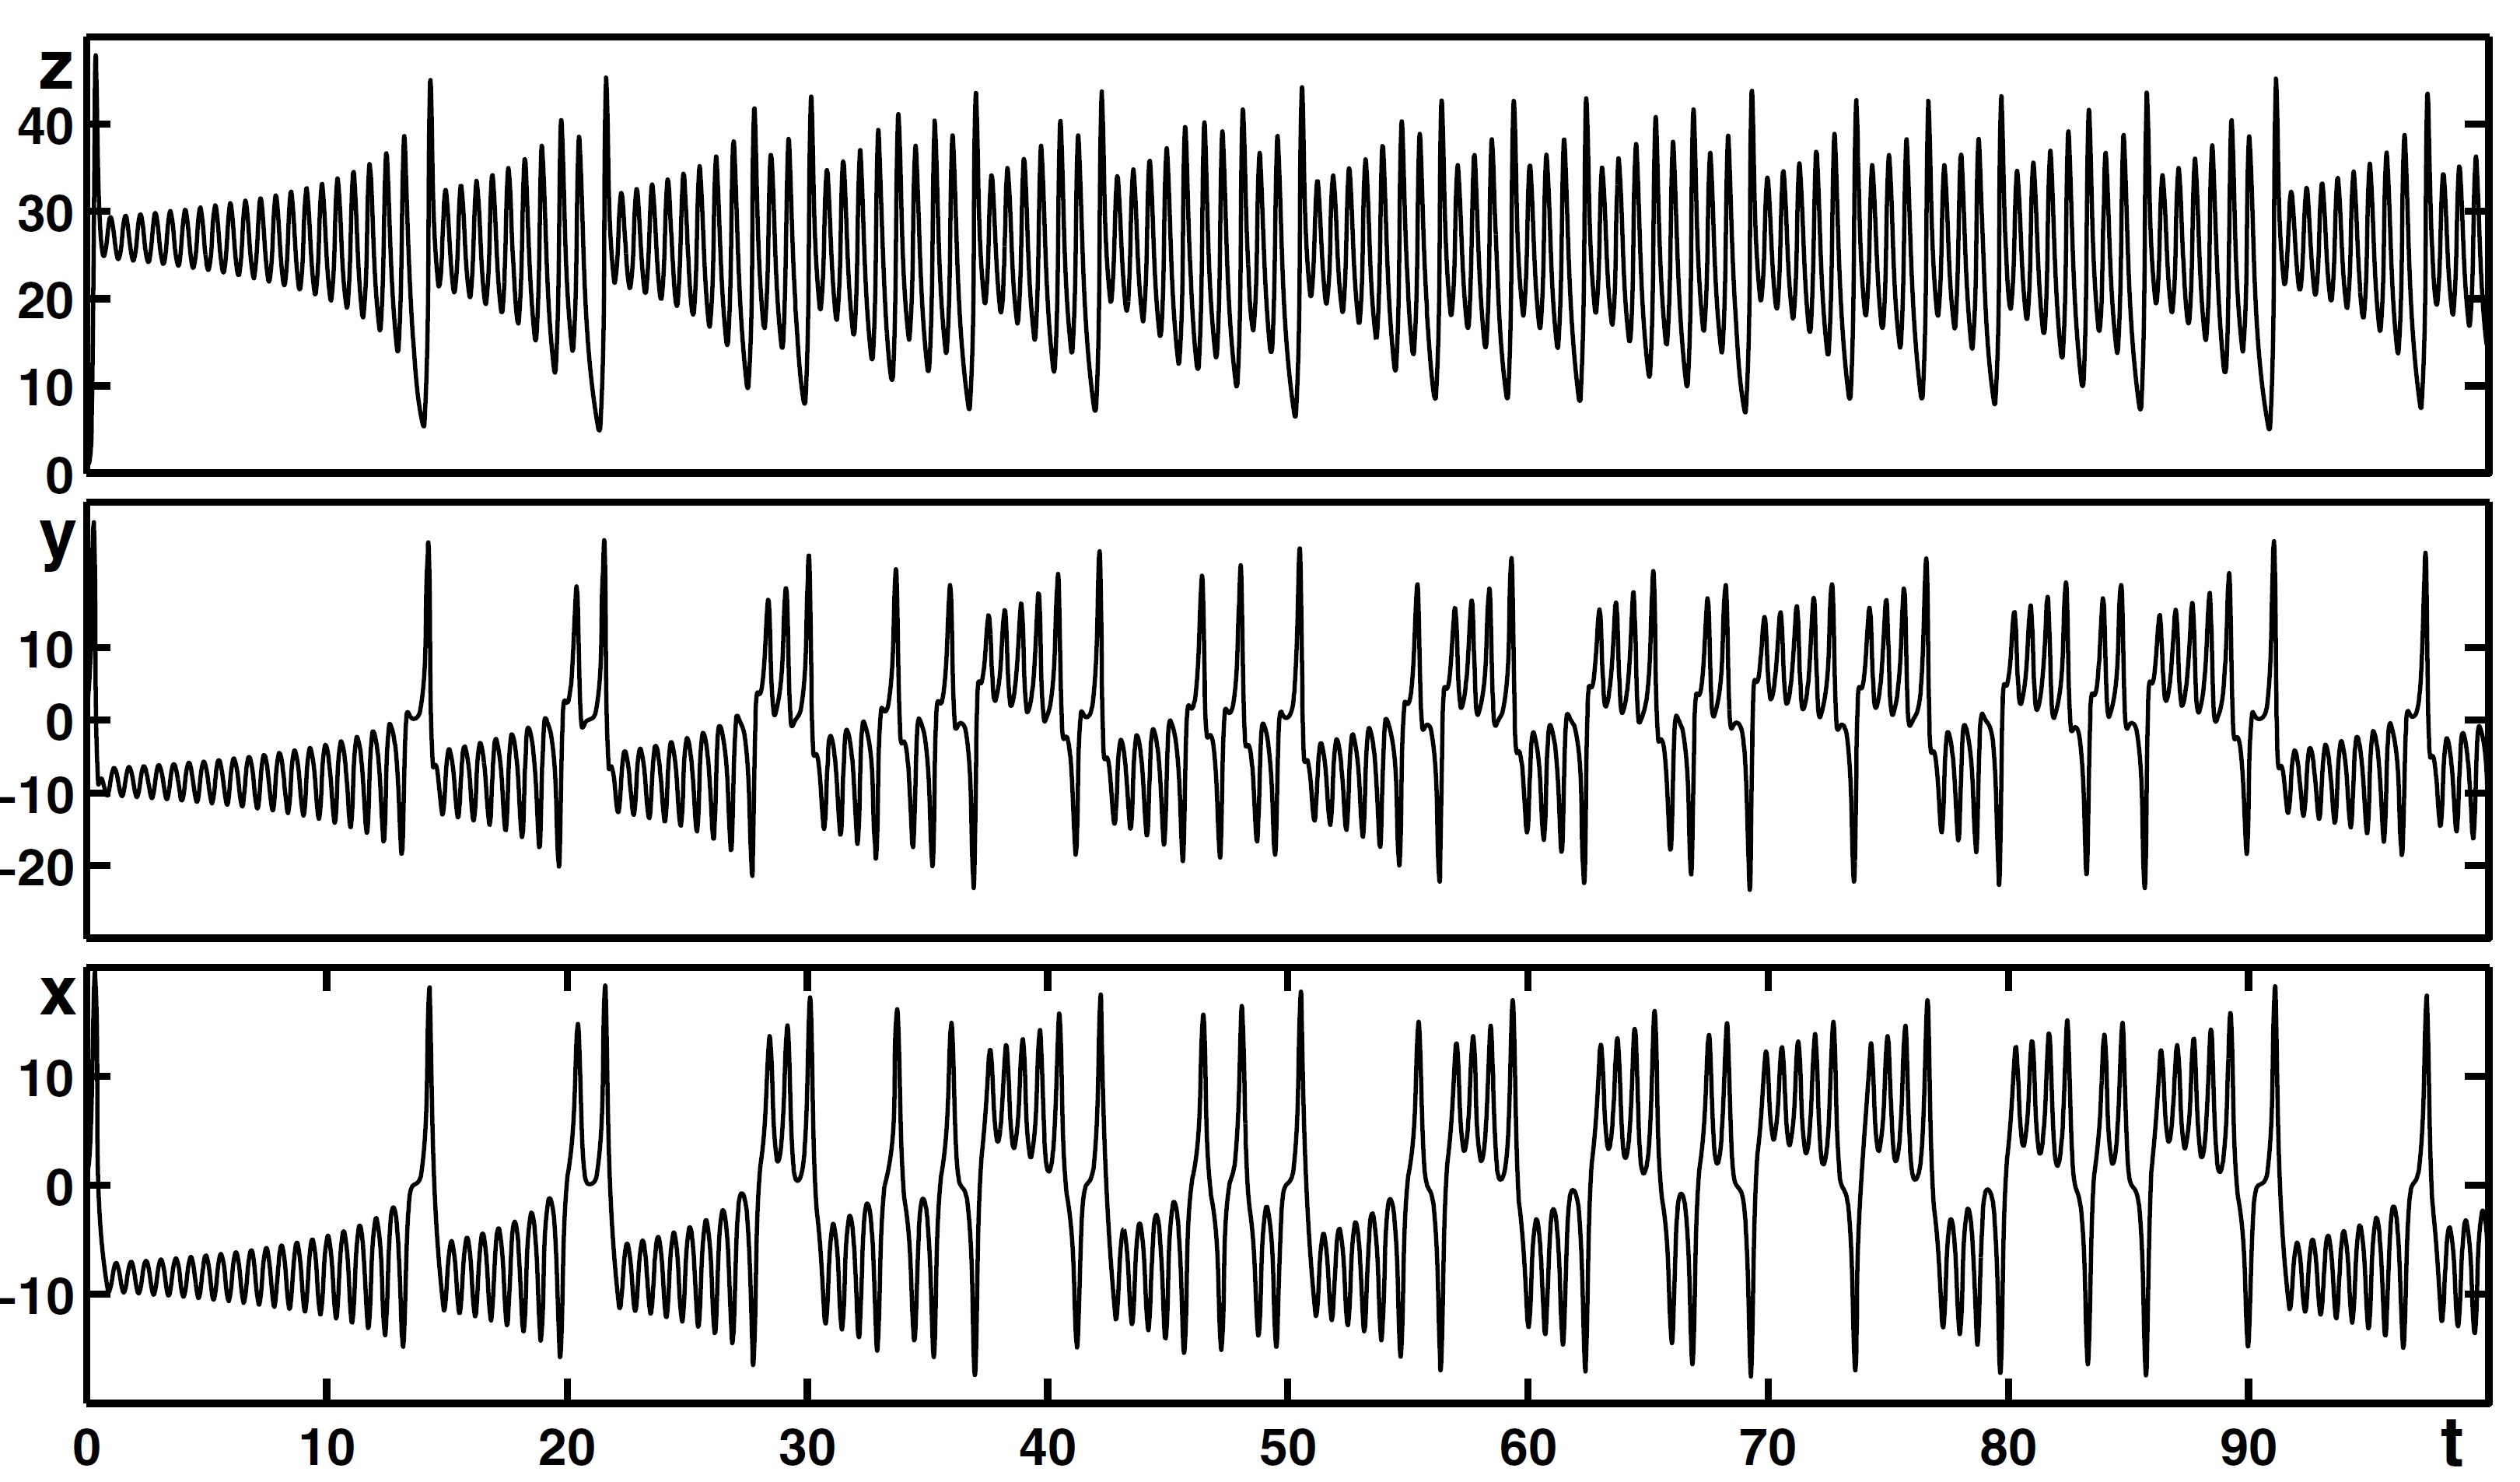
\includegraphics[width=\linewidth]{tsls.png}
	\caption{Time series for the Lorenz system for $\sigma=10, b=\frac{8}{3}$ and $r=28$.}
	\label{fig:tsls}
	\end{subfigure}
	\vline
	\begin{subfigure}{0.45\linewidth}
	\centering
	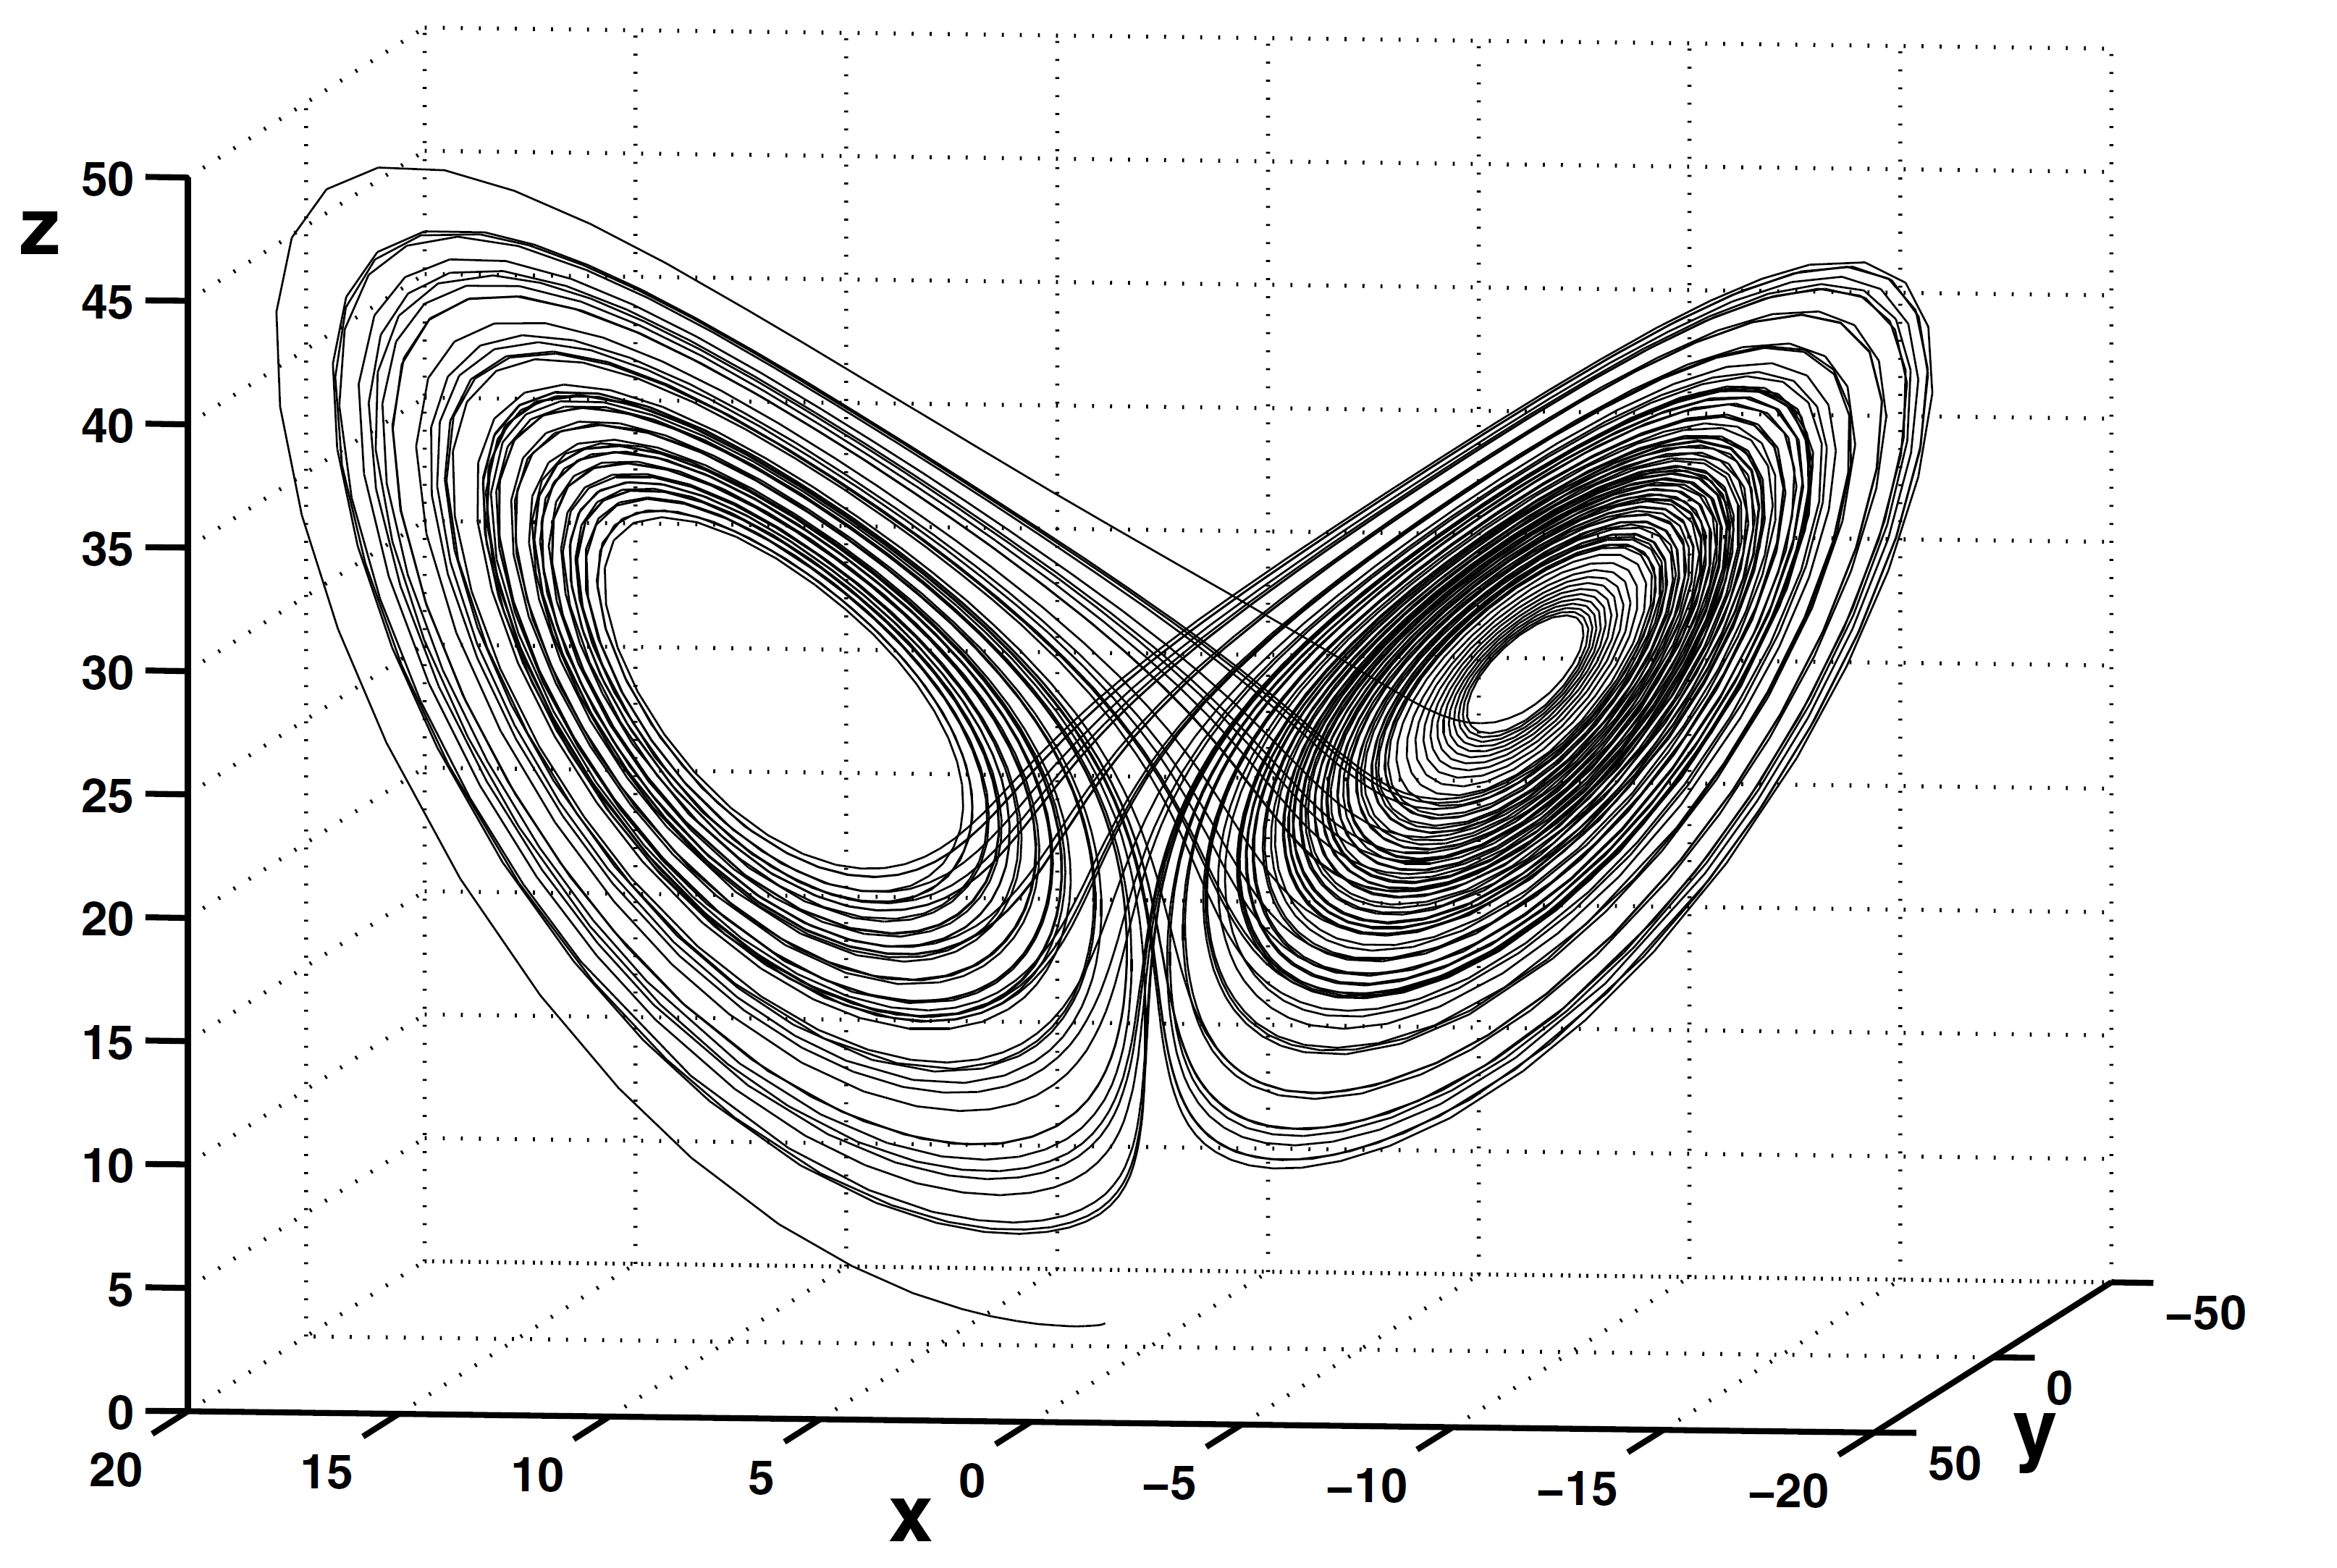
\includegraphics[width=\linewidth]{lals.png}
	\caption{The Lorenz attractor as a three-dimensional plot of the time series (Figure (\ref{fig:tsls}))}
	\label{fig:lals}
	\end{subfigure}
	\end{figure}
\end{comment}
The Lorenz attractor consists of two sheets roughly defined by planes for positive and negative values of $x$ where the trajectory spirals outwards with the fixed points $\mathbf{\tilde{x}}_{2,3}$ located at the centers of these spirals.
\begin{figure}[h!]
	\centering
	\begin{subfigure}{0.45\linewidth}
		\centering
		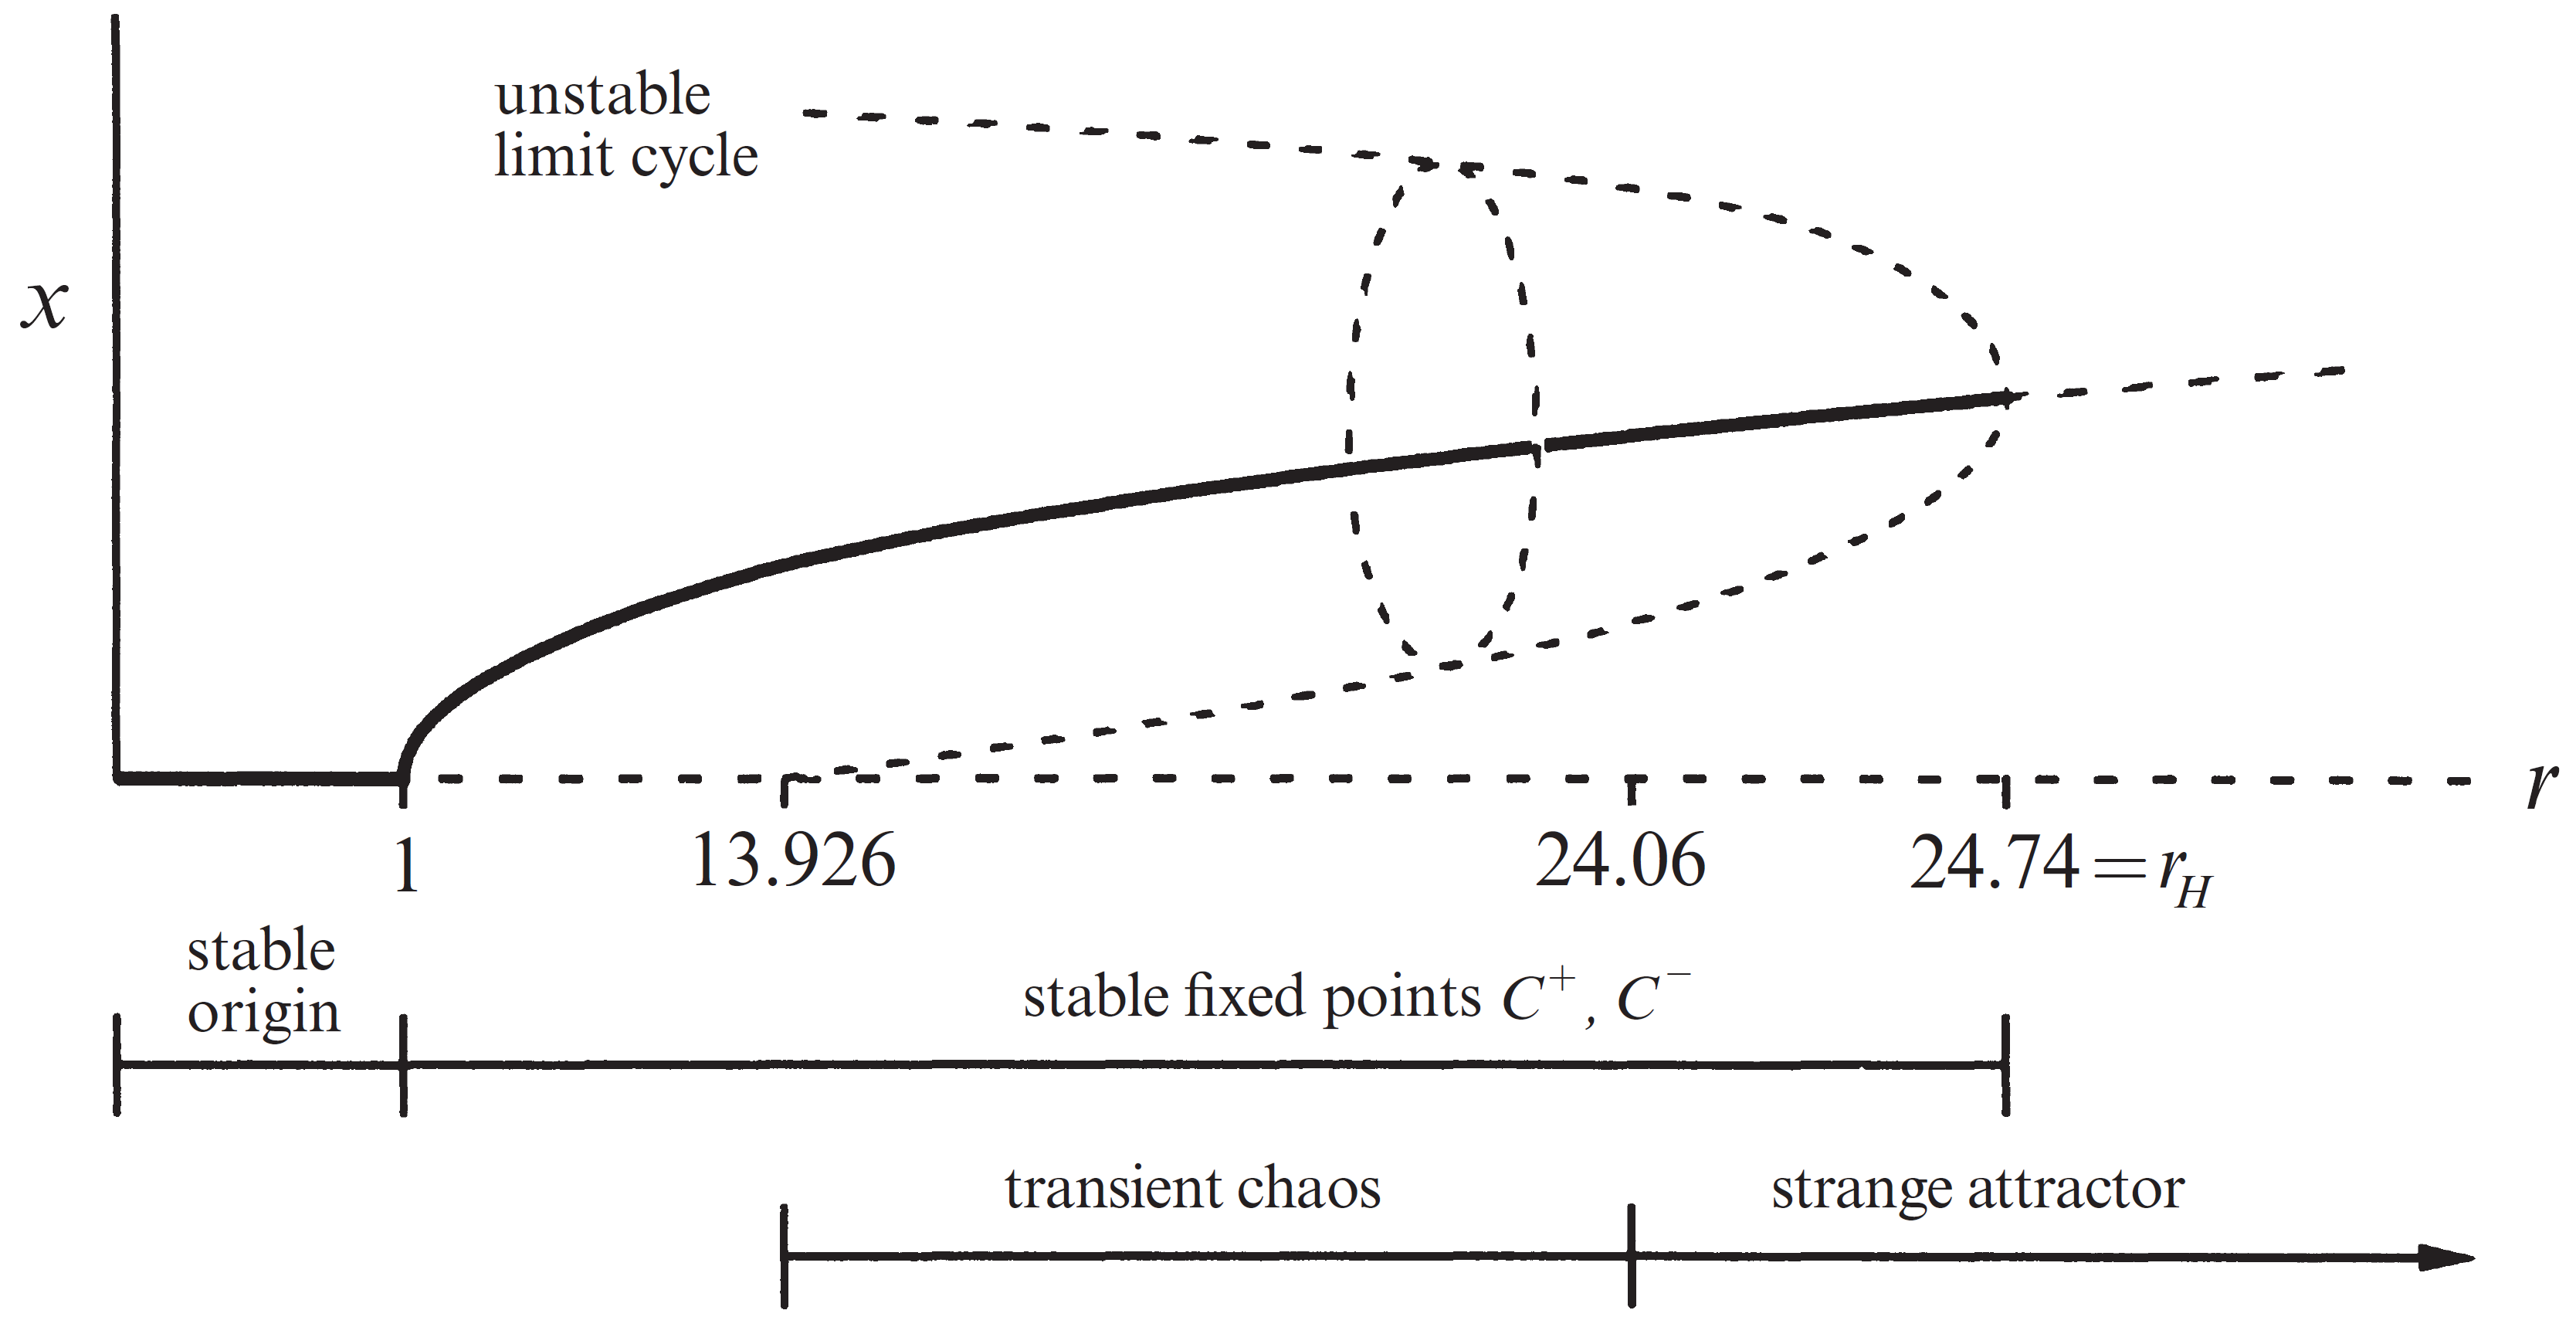
\includegraphics[width=\linewidth]{bfls.png}
		\caption{Parameter Space of Lorenz System}
		\label{fig:bfls}
	\end{subfigure}
	\vline
	\begin{subfigure}{0.45\linewidth}
		\centering
		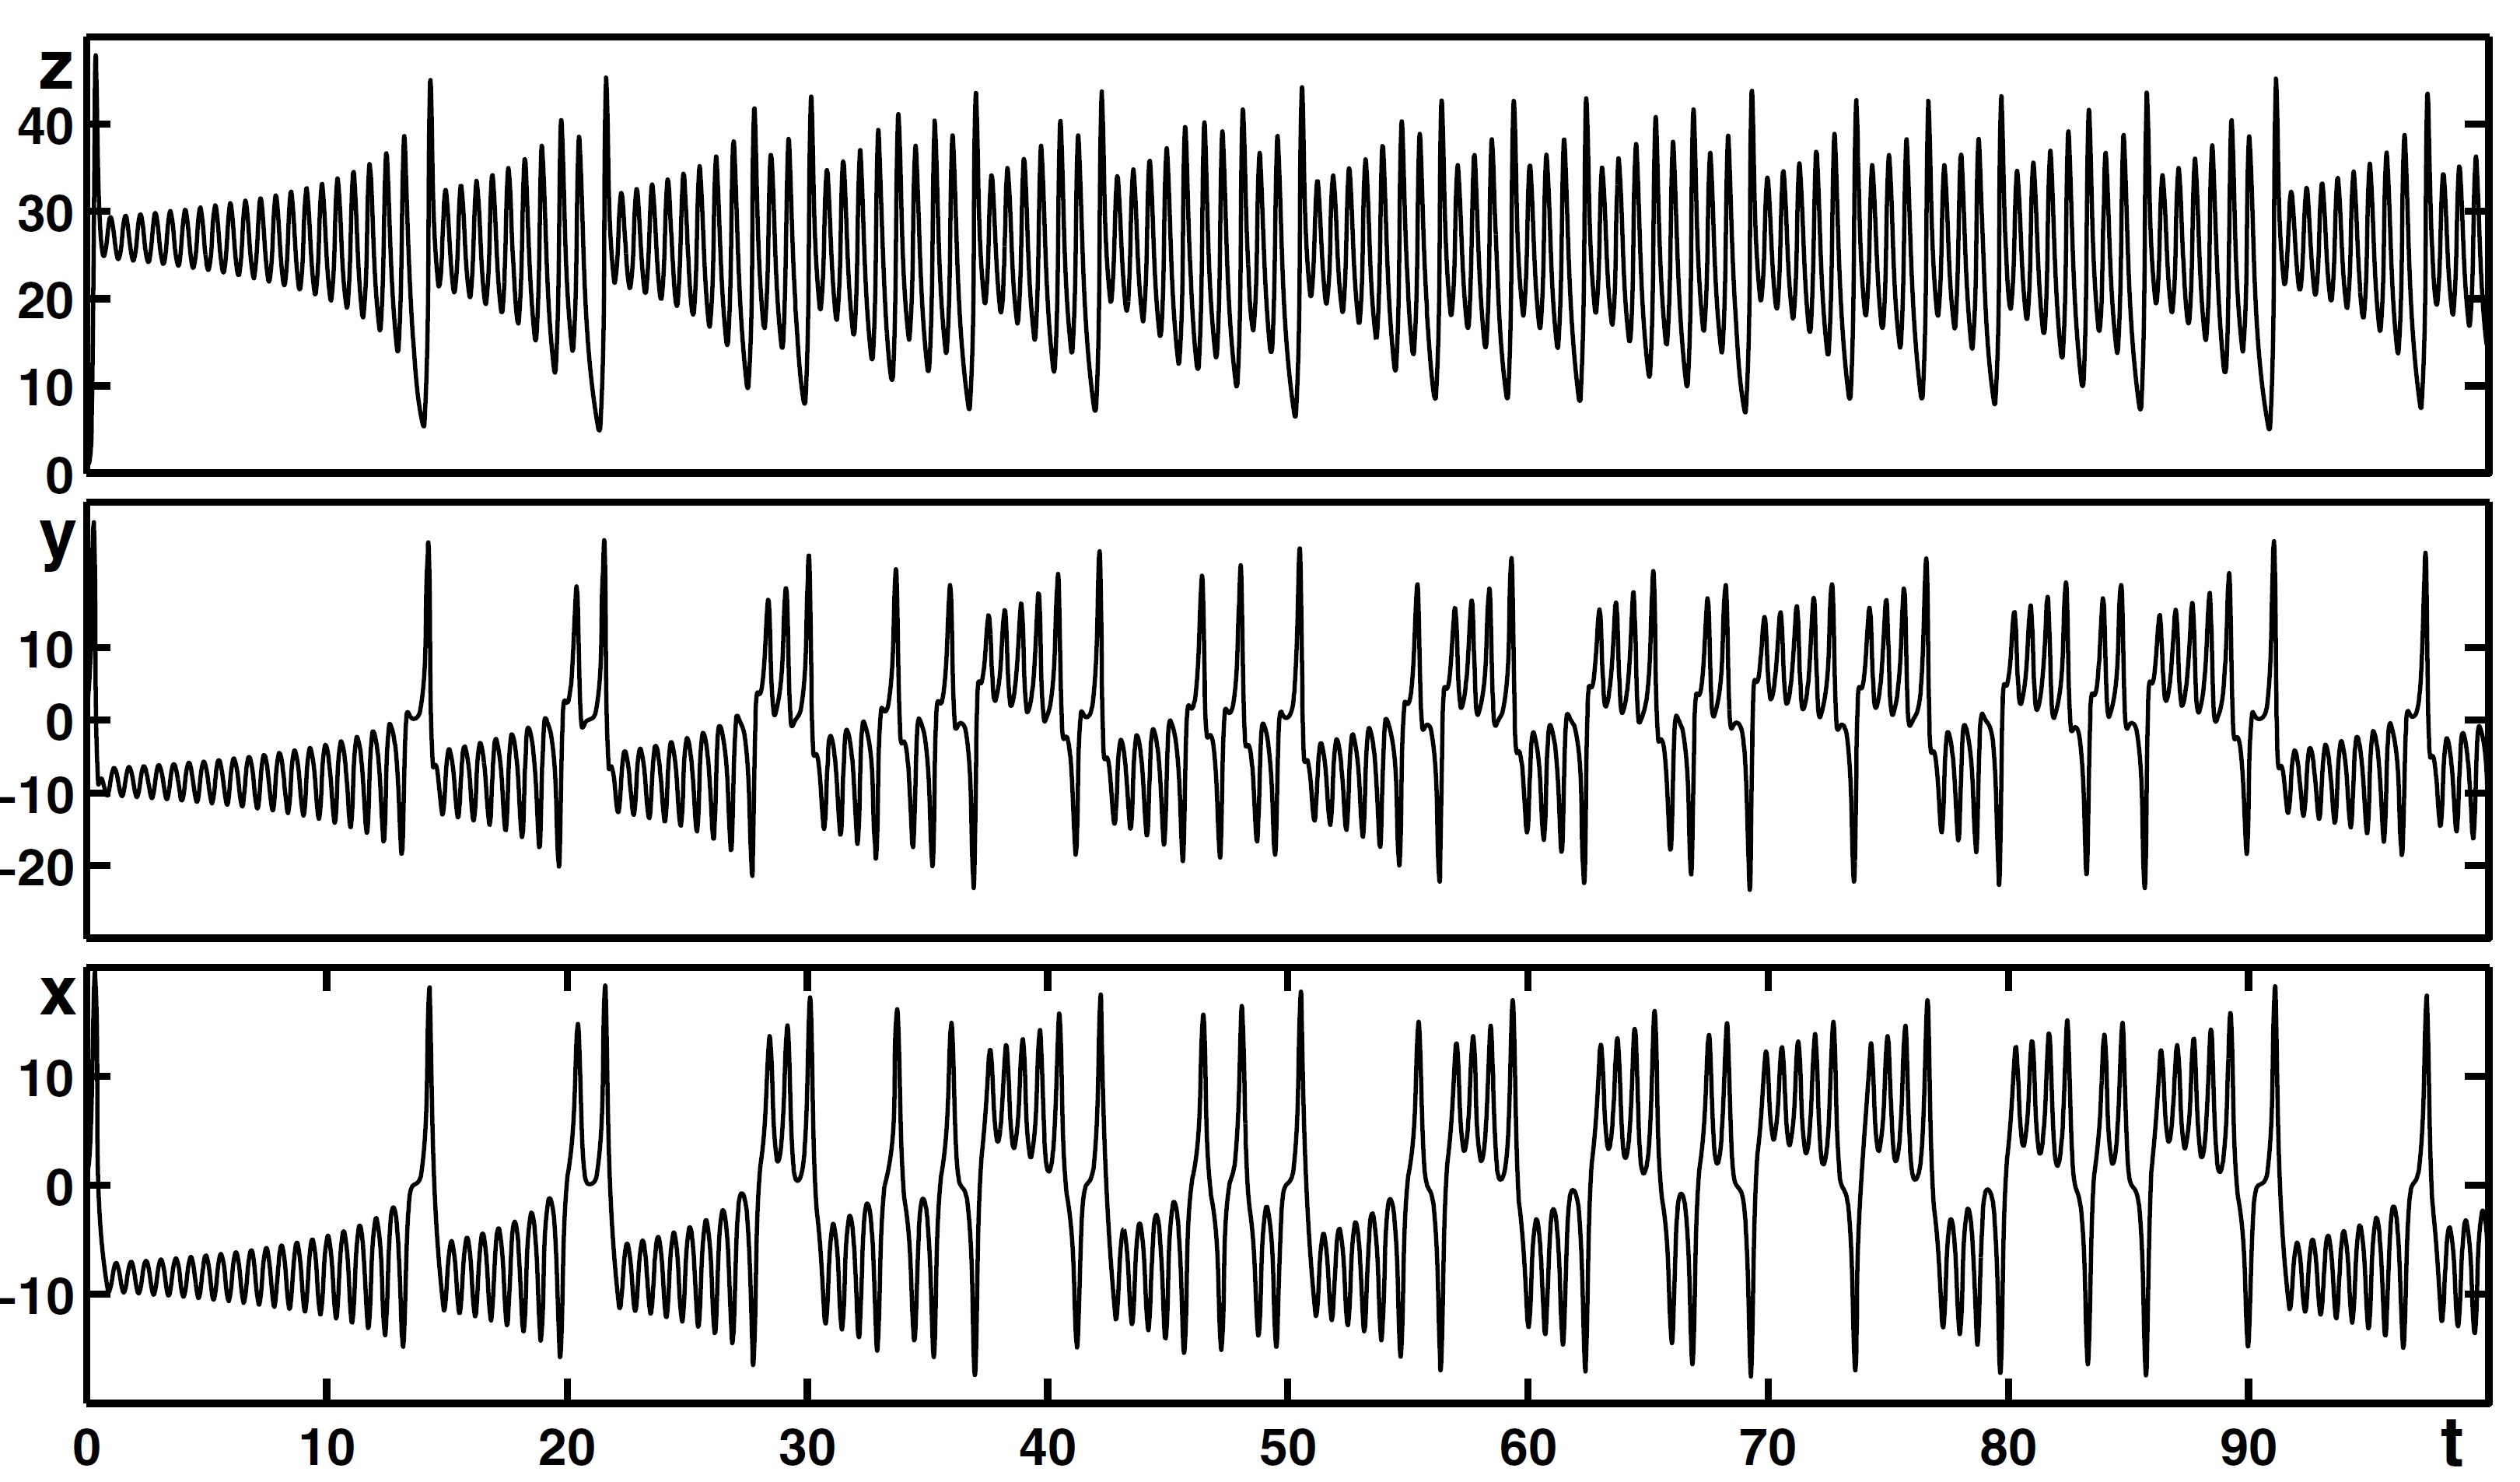
\includegraphics[width=\linewidth]{tsls.png}
		\caption{Time series for the Lorenz system for $\sigma=10, b=\frac{8}{3}$ and $r=28$.}
		\label{fig:tsls}
	\end{subfigure}
\end{figure}
\begin{figure}[h!]
	\centering
	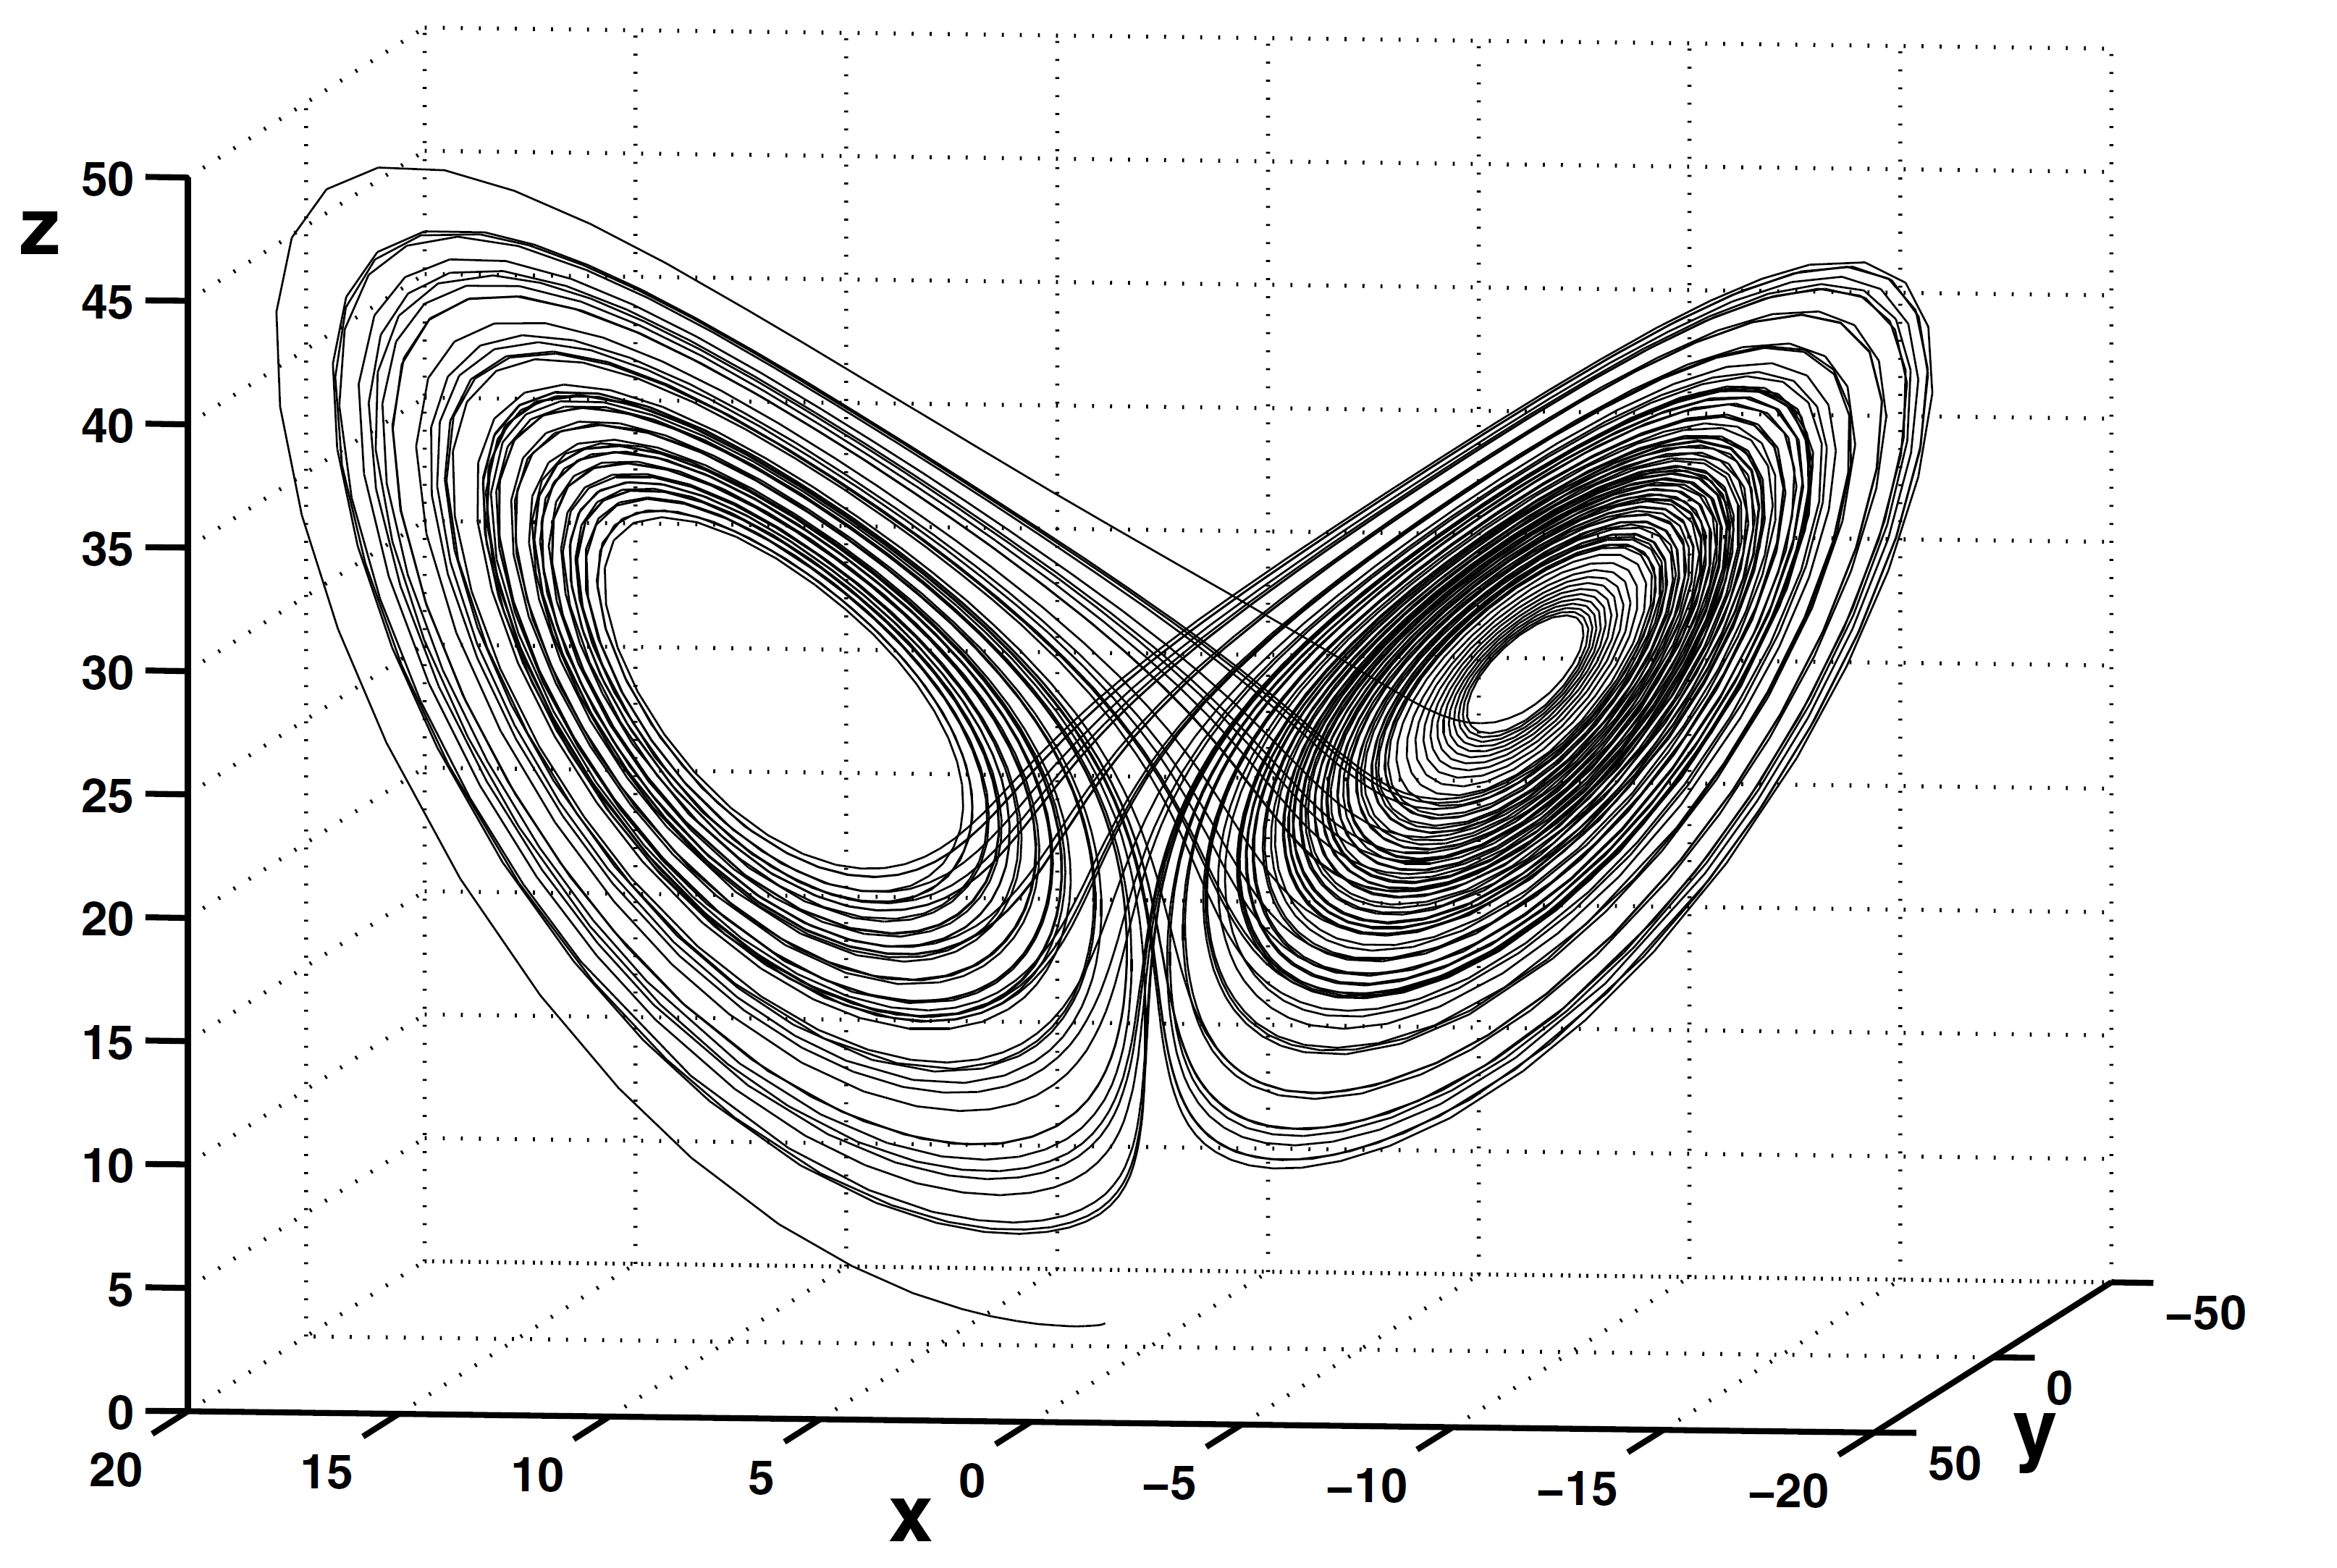
\includegraphics[width=0.7\linewidth]{lals.png}
	\caption{The Lorenz attractor as a three-dimensional plot of the time series (Figure (\ref{fig:tsls}))}
	\label{fig:lals}
\end{figure}
\subsubsection{Properties of Strange Attractor}
\begin{itemize}
	\item The trajectory is aperiodic.
	\item The trajectory remains on the attractor forever. (the attractor is \emph{invariant})
	\item The general form is independent of initial conditions.
	\item The sequence of windings is sensitive to initial conditions.
	\item The attractor has fractal structure.
\end{itemize}
\subsection{R\"ossler System}{\label{sec:rs}}
The R\"ossler system with its standard parameters for chaotic behavior is given by
\begin{equation}
	\begin{aligned}
		\dot{x}&=-y-z\\
		\dot{y}&=x+ay\\
		\dot{z}&=b+z(x-c)
	\end{aligned}\quad\text{with}\quad
	a=b=0.2
\end{equation}
The dynamics of the R\"ossler system consist of a spiral movement in the $xy-$plane and escapes along the positive $z-$direction.
A three-dimensional plot of the R\"ossler attractor together with the time series for the $x-, y-$ and $z-$coordinates are shown in Figure (\ref{fig:rars}).
For $a=b=0.2$ kept fixed and varying $c$ the R\"ossler system undergoes a sequence of period doublings from a simple limit cycle at $c =2.5$ to a strange attractor at $c = 5$.
Beyond this first chaotic r\`egime there are again limit cycles that bifurcate into orbits of increasing complexity, before the standard attractor at $c=5.7$ is reached.
\begin{figure}[h!]
	\centering
	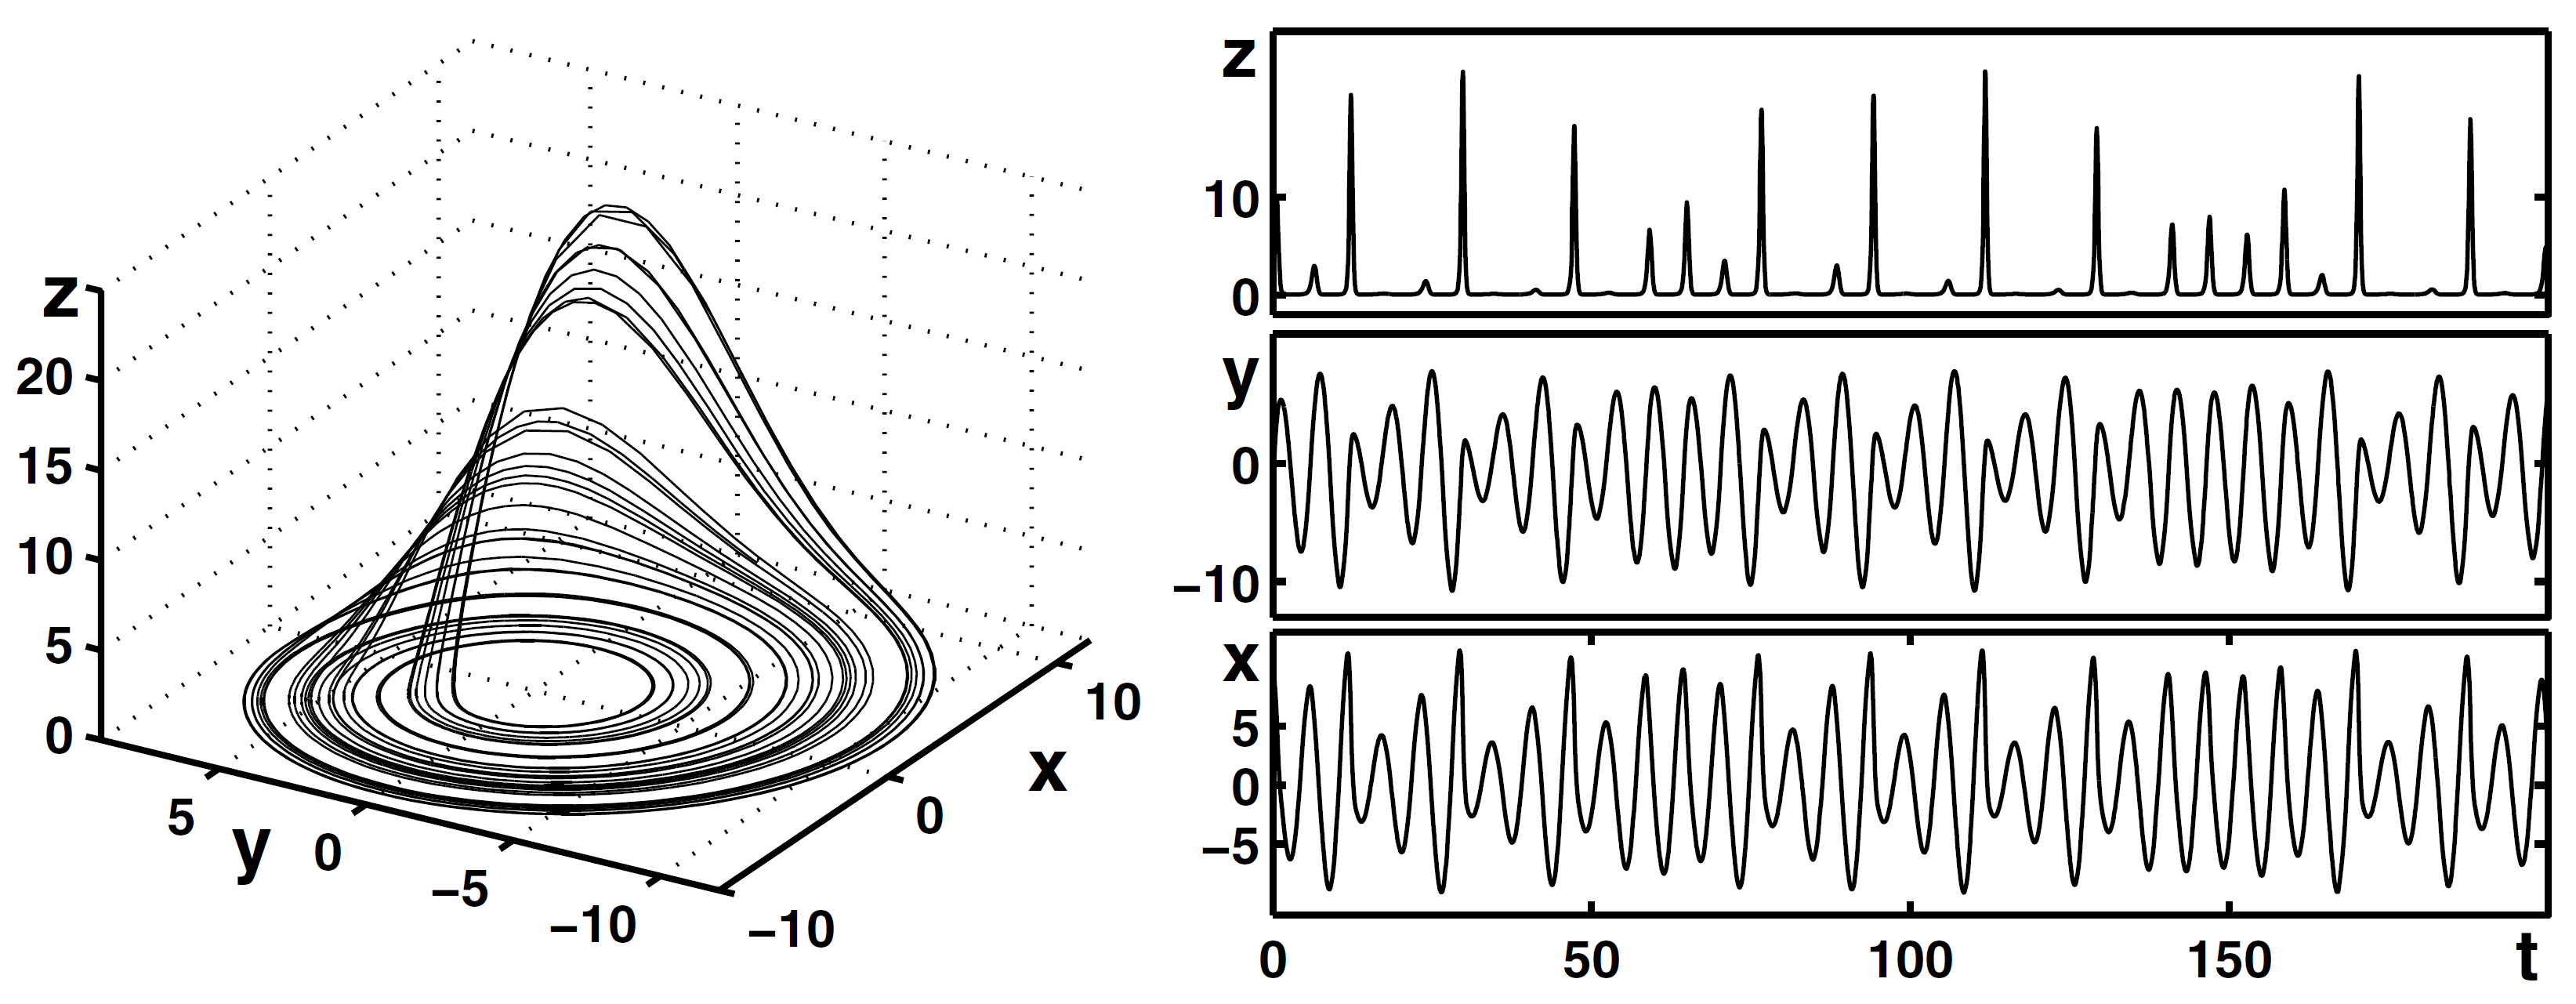
\includegraphics[width=\linewidth]{rars.png}
	\caption{The R\"ossler attractor in a three-dimensional plot (left) and time series of the corresponding $x-, y-$ and $z-$coordinates (right).\\Parameters: $a=b=0.2, c =5.7$.}
	\label{fig:rars}
\end{figure}

\section{Lyapunov Exponents For Continous Systems}
Strange attractors can be characterized by a measure that describes how the distance between adjacent trajectories changes in time.
\begin{figure}
	\centering
	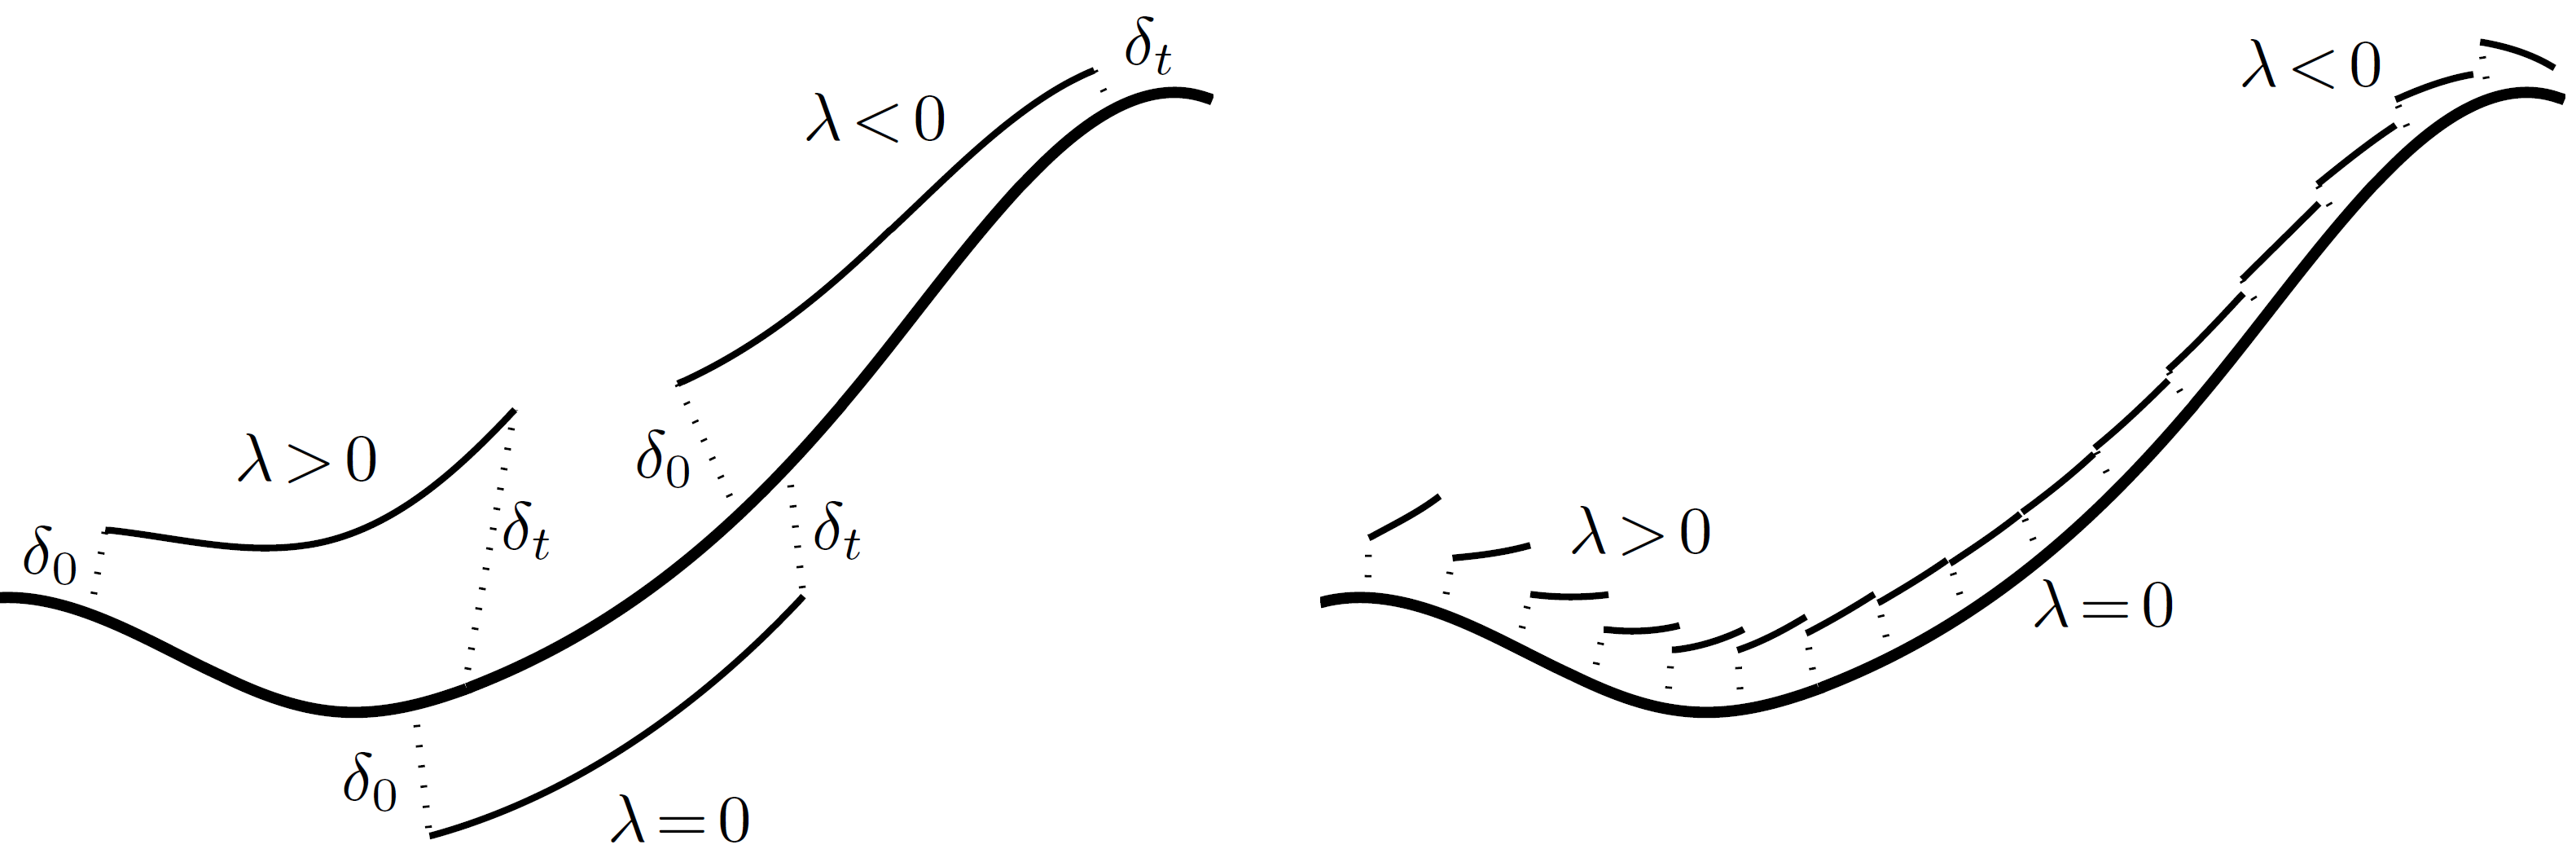
\includegraphics[width=0.7\linewidth]{lye.png}
	\caption{Left: Diverging, parallel and converging trajectories correspond to a local divergence rate of $\lambda>0, \lambda=0$ and $\lambda<0$, respectively.\\ Right: A Lyapunov exponent is determined as an average of the local divergence rate following close-by trajectories around the attractor.}
	\label{fig:lye}
\end{figure}
An example is shown in Figure (\ref{fig:lye} (left))  for the cases of diverging, parallel and converging trajectories.
For small initial distances $\delta_0$ and short times $t$ this behavior is determined by the local linearization. The distance between the two trajectories as a function of time is then given by
\begin{equation}
	\delta(t)=\delta_0e^{\lambda t}\quad\rightarrow\quad
	\lambda=\frac{1}{t}\ln\frac{\delta(t)}{\delta_0}
\end{equation}
where for $\lambda>0$ the trajectories are diverging, for $\lambda<0$ they are converging and for $\lambda=0$ the distance between corresponding points on the two trajectories does not change.
The exponent $\lambda$ is called the \emph{local divergence rate}, and as the name indicates, is a local quantity.\\
A global characterization is found by averaging the local divergence rate obtained from small segments of a trajectory over a long time by applying the procedure indicated in Figure (\ref{fig:lye} (right)).
In general, the sum over all Lyapunov exponents is negative for any attractor.
{\renewcommand{\arraystretch}{1.2}
\begin{table}[h!]
	\centering
	\caption{Classification of attractors in three dimensions.}
	\label{tab:catd}
	\begin{tabular}{c c c c}
		Type&$1^{st}$ exponent&$2^{nd}$ exponent&$3^{rd}$ exponent\\
		\hline
		Fixed Point&$-$ve&$-$ve&$-$ve\\
		Periodic orbit&0&$-$ve&$-$ve\\
		Quasi-Periodic orbit&0&0&$-$ve\\
		Strange attractor&$+$ve&0&$-$ve\\
		Lorenz attractor&0.906&0&$-$14.57\\
		R\"ossler attractor&0.0714&0&$-$5.39\\
	\end{tabular}
\end{table}}
\begin{theorem}[\textbf{Lyapunov Exponents}]
	If at least one of the average Lyapunov exponents is \emph{positive}, then the system is \textbf{chaotic}; if the average Lyapunov exponent is \emph{negative}, then the orbit is \textbf{periodic} and when the average Lyapunov exponent is \emph{zero}, a \textbf{bifurcation} occurs.
\end{theorem}

\newpage
\part{Discrete Dynamical Systems}

\section{Linear Discrete Systems}
\input{Sections/Linear Discrete Systems }

\section{Analysis}{\label{sec:dds}}
\subsection{Linear Stability in One Dimension}
Consider a nearby orbit $x_n=\tilde{x}+\xi_n$ for a fixed point $\tilde{x}$
\begin{equation}
	\xi_{n+1}+\tilde{x}=f(x_n)\approx f(\tilde{x})+f^\prime(\tilde{x})\ \xi_n+\frac{1}{2!}f^{\prime\prime}(\tilde{x})\xi_n^2+\cdots
\end{equation}
$f(\tilde{x})=\tilde{x}$ as it is a fixed point.
$|\xi_n|$ is small as we assume to be in the vicinity of $\tilde{x}$, and therefore $\xi_n^2$ is tiny and can be neglected.
with \emph{eigenvalue} or {\textbf{multiplier}} $\lambda=f^\prime(\tilde{x})$
\begin{equation}
	\xi_{n+1}=f^\prime(\tilde{x})\ \xi_n=\lambda\ \xi_n\quad\rightarrow\quad\xi_n=\lambda^n\xi_0
\end{equation}
If $|\lambda|<1$, then fixed point $\tilde{x}$ is \textbf{linearly stable}.
For positive values of $\lambda$, $\xi_i=0$ is approached \emph{monotonically}, for a negative $\lambda$ the values of $\xi_i$ \emph{alternate} between positive and negative after each iteration step.
Conversely, if $|\lambda|>1$ then the fixed point is {\textbf{unstable}}.
\subsection{Graphical Iteration (Cobwebs)}
The general method for determining the itinerary of a seed $x_0$ for a function $f(x)$ is as follows
\begin{itemize}
	\item Start with the seed $x_0$ on the $x$-axis.
	\item Move up to the function $f(x)$.
	\item Move horizontally (left or right) to the $y=x$ line.
	\item Move vertically (up or down) to the function $f(x)$
	\item Repeat above two steps again and again.
\end{itemize}
Consider the \textbf{Tent Map} $T:[0,1]\rightarrow[0,1]$ defined by
\begin{equation}
	T(x)=
	\begin{cases}
		\mu x&0\leq x<\frac{1}{2}\\
		\mu(1-x)&\frac{1}{2}\leq x\leq1
	\end{cases}
\end{equation}
\begin{figure}[h!]
	\centering
	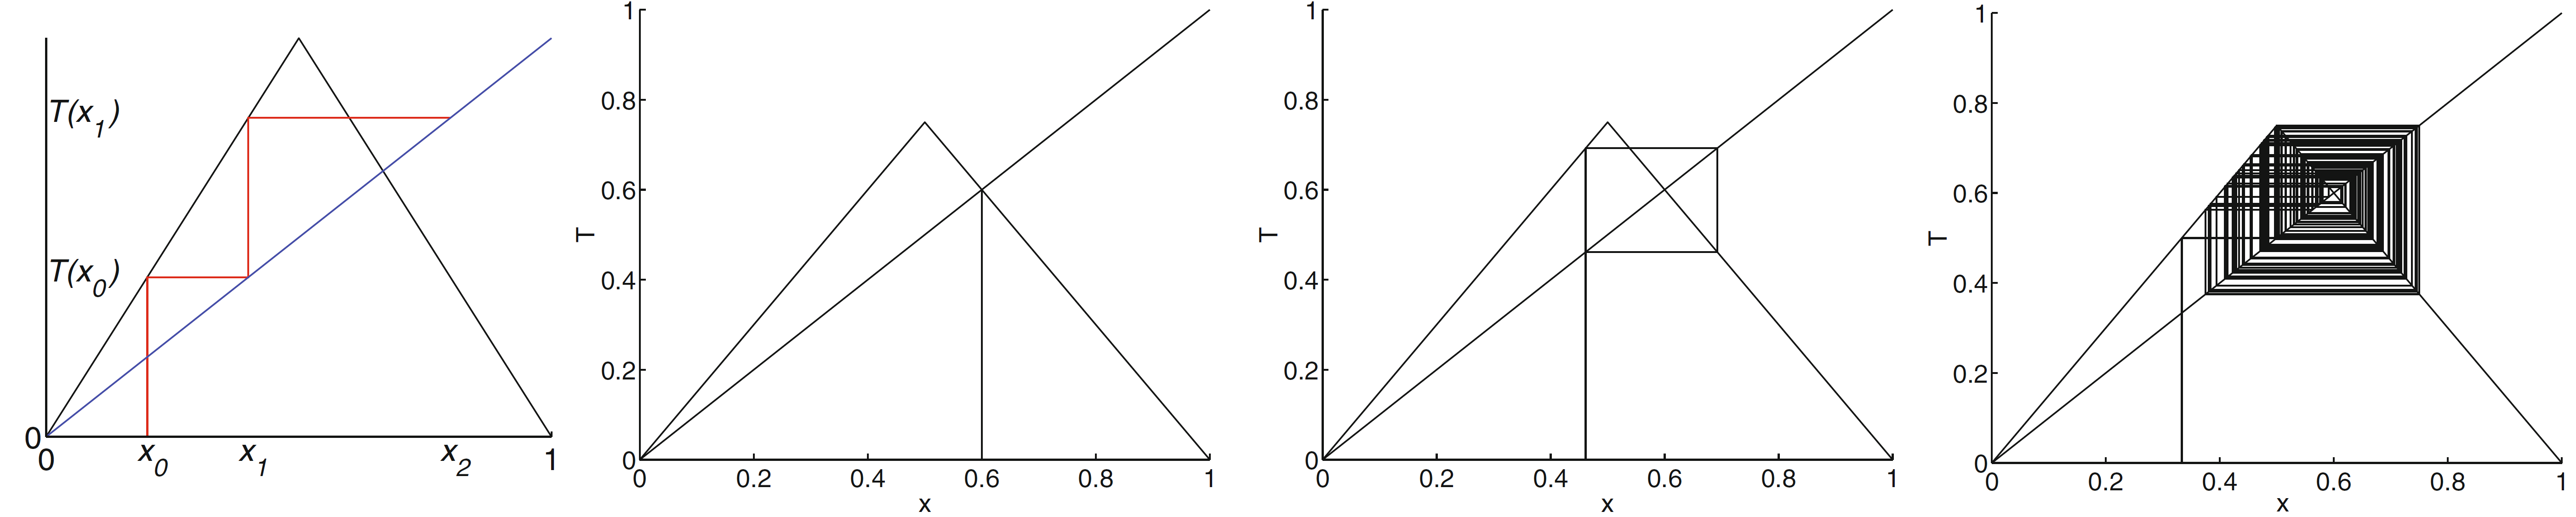
\includegraphics[width=0.83\linewidth]{cwd.png}
	\caption{a) A possible graphical iteration when n =2.\\Graphical iterations when $\mu=\frac{3}{2}$: b) $x_0=\frac{3}{5}$ c) $x_0=\frac{6}{13}$ d) $x_0=\frac{1}{3}$, for 200 iterations.}
	\label{fig:cwd}
\end{figure}

\section{Logistic Map}{\label{sec:lm}}
The easiest and best studied nonlinear map is the \emph{logistic map} defined as
\begin{equation}
	x_{n+1}=Ax_n(1-x_n)=A(x_n-x_n^2)\quad\text{with}\quad0\leq A\leq4
\end{equation}
\textbf{fixed points} for map is $x_{n+1}=x_n$.
\begin{equation}
	x_n=A(x_n-x_n^2)\quad\rightarrow\quad\tilde{x}_1=0\quad\tilde{x}_2=\frac{A-1}{A}
\end{equation}
As before, we can linearize around these fixed points to determine their stability
\begin{equation*}
	\xi_{n+1}\approx\underbrace{A(1-2\tilde{x})}_{\tilde{A}}\xi_n=\tilde{A}\ \xi_n
\end{equation*}
For the two fixed points $\tilde{x}_1$ and $\tilde{x}_2$ we find
\begin{equation}
	\begin{aligned}
		\tilde{x}_1=0\quad\rightarrow\quad\tilde{A}=A\quad\rightarrow\quad\text{stable for}\ 0\leq A<1\\
		\tilde{x}_2=1-\frac{1}{A}\quad\rightarrow\quad\tilde{A}=A\left\{1-2\left(\frac{A-1}{A}\right)\right\}=2-A\quad\rightarrow\quad\text{stable for}\ 1\leq A\leq3
	\end{aligned}
\end{equation}
These fixed points and their stability can be seen in the bifurcation diagram shown in Figure (\ref{fig:lmbf}).\\
By varying the parameter $A$, the following behavior is observed:
\begin{itemize}
	\item With $A$ between 0 and 1, $x_n\rightarrow0$ as $n\rightarrow\infty$ independent of $x_0$.
	\item With $A$ between 1 and 2, $x_n\rightarrow\dfrac{A-1}{A}$ as $n\rightarrow\infty$ independent of $x_0$.
	\item With $A$ between 2 and 3, $x_n\rightarrow\dfrac{A-1}{A}$ as $n\rightarrow\infty$ but it will fluctuate around that value for some time (converges linearly).
	\begin{figure}[h!]
		\centering
		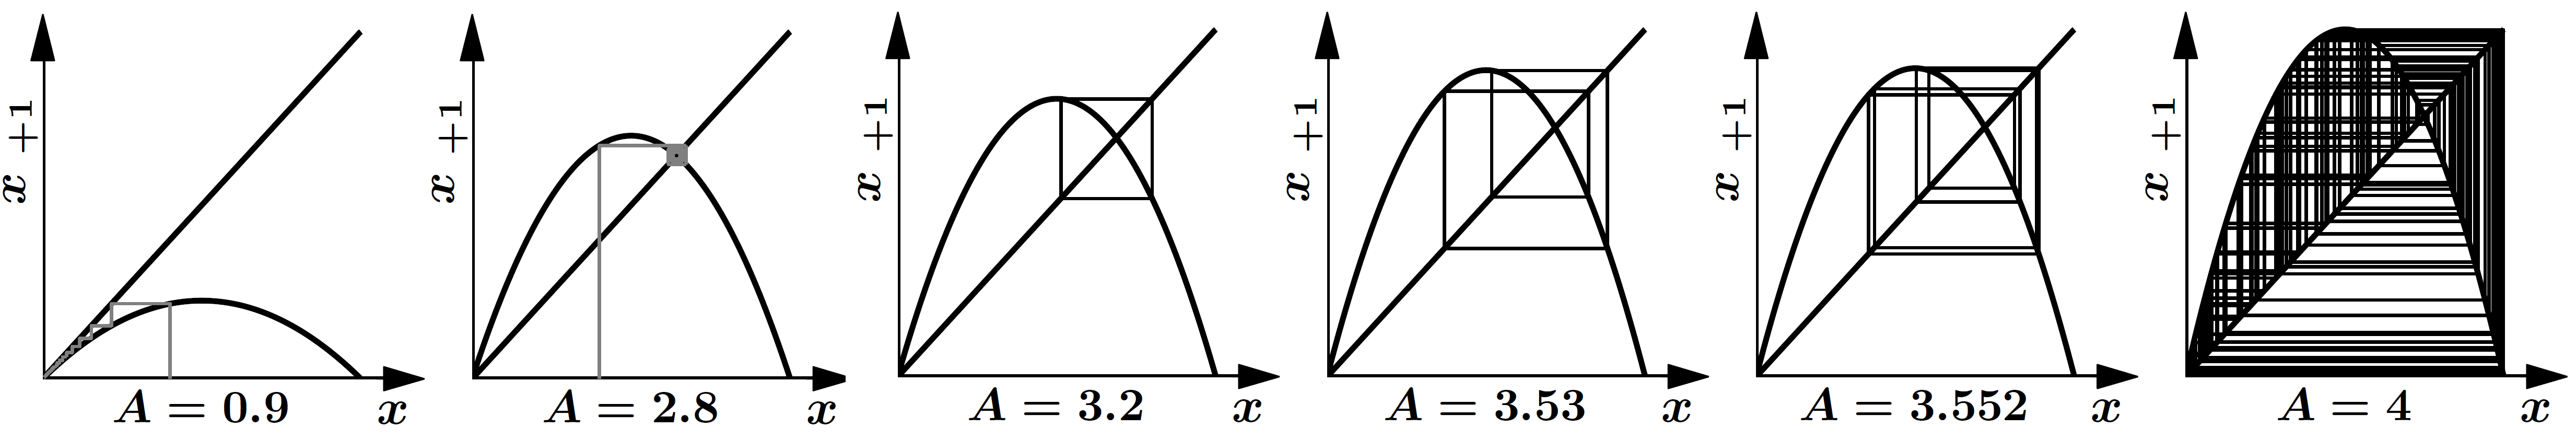
\includegraphics[width=\linewidth]{lm34.png}
		\caption{Stationary states from left to right are fixed points 0 and $\frac{9}{14}$ then orbits with periods of 2, 4 and 8, as well as a chaotic trajectory.}
		\label{fig:lm34}
	\end{figure}
	\item In discrete maps, the analogue to limit cycles in differential equations are periodic orbits of period $m$, where $x_{n+m}=x_n$ is fulfilled.
	Orbits of period 2 are solutions with $x_{n+2}=x_n$
	\begin{equation}
		x_{n+2}=f^{(2)}(x_n)=A^2x_n(1-x_n)(1-Ax_n+Ax_n^2)
	\end{equation}
	The function $f^{(2)}(x_n)$ is called the \emph{second iterate} and has the fixed points
	\begin{equation}
		\tilde{x}_1=0\quad\tilde{x}_2=1-\frac{1}{A}\quad\tilde{x}_{3,4}=\frac{1}{2A}\left\{A+1\pm\sqrt{A^2-2A-3}\right\}
	\end{equation}
	The points $\tilde{x}_1$ and $\tilde{x}_2$ are the fixed points of the map we know already and are unstable for $A>3$.
	It can be shown that the period-2 solution is stable for $3<A<1+\sqrt{6}$.\\
	With $A$ between 3 and $1+\sqrt{6}\approx3.44949$, from almost all $x_0$, $x_n$ will approach permanent oscillations between two values dependent on $A$.
	\item With $A$ between $1+\sqrt{6}$ and 3.54409 (approximately\footnote{This is a root of a $12^{th}$ degree polynomial $4913 + 2108x^2 - 604x^3 - 977x^4 + 8x^5 + 44x^6 + 392x^7 - 193x^8 - 40x^9 + 48x^{10} - 12x^{11} + x^{12}$! So we turn to approximations. :-(}), from almost all $x_0$, $x_n$ will approach permanent oscillations among four values. 
	\item With $A$ increasing beyond 3.54409, from almost all initial conditions $x_0$ will approach oscillations among 8 values.
	This period doubling behavior continues until a period-$\infty$ is reached at a parameter value of $A\approx3.569945672$ and is called \textbf{period-doubling cascade}.
	\item Beyond this point till $A=4$, there is a region of deterministic chaos where the solution is a strange attractor.
	Evidently, this structure in parameter space is a kind of replication of the whole bifurcation diagram on a smaller scale in $x$ and $A$, a feature called \emph{self-similarity}.\\
	This is not the end of the story, however, Figure (\ref{fig:lmbf}) clearly shows regions where the system returns to periodic behavior, even if for only a small range of $\mu$ values.
	These regions are called \textbf{periodic windows}.
	\item The special case of r = 4 can in fact be solved exactly
	\begin{equation}
		x_n=\sin^2(2^n\theta\pi)\quad\text{where}\quad\theta=\frac{1}{\pi}\sini(\sqrt{x_0})
	\end{equation}
	\item Beyond $A=4$, almost all initial values eventually leave the interval $[0,1]$ and diverge.
\end{itemize}
\begin{figure}[h!]
	\centering
	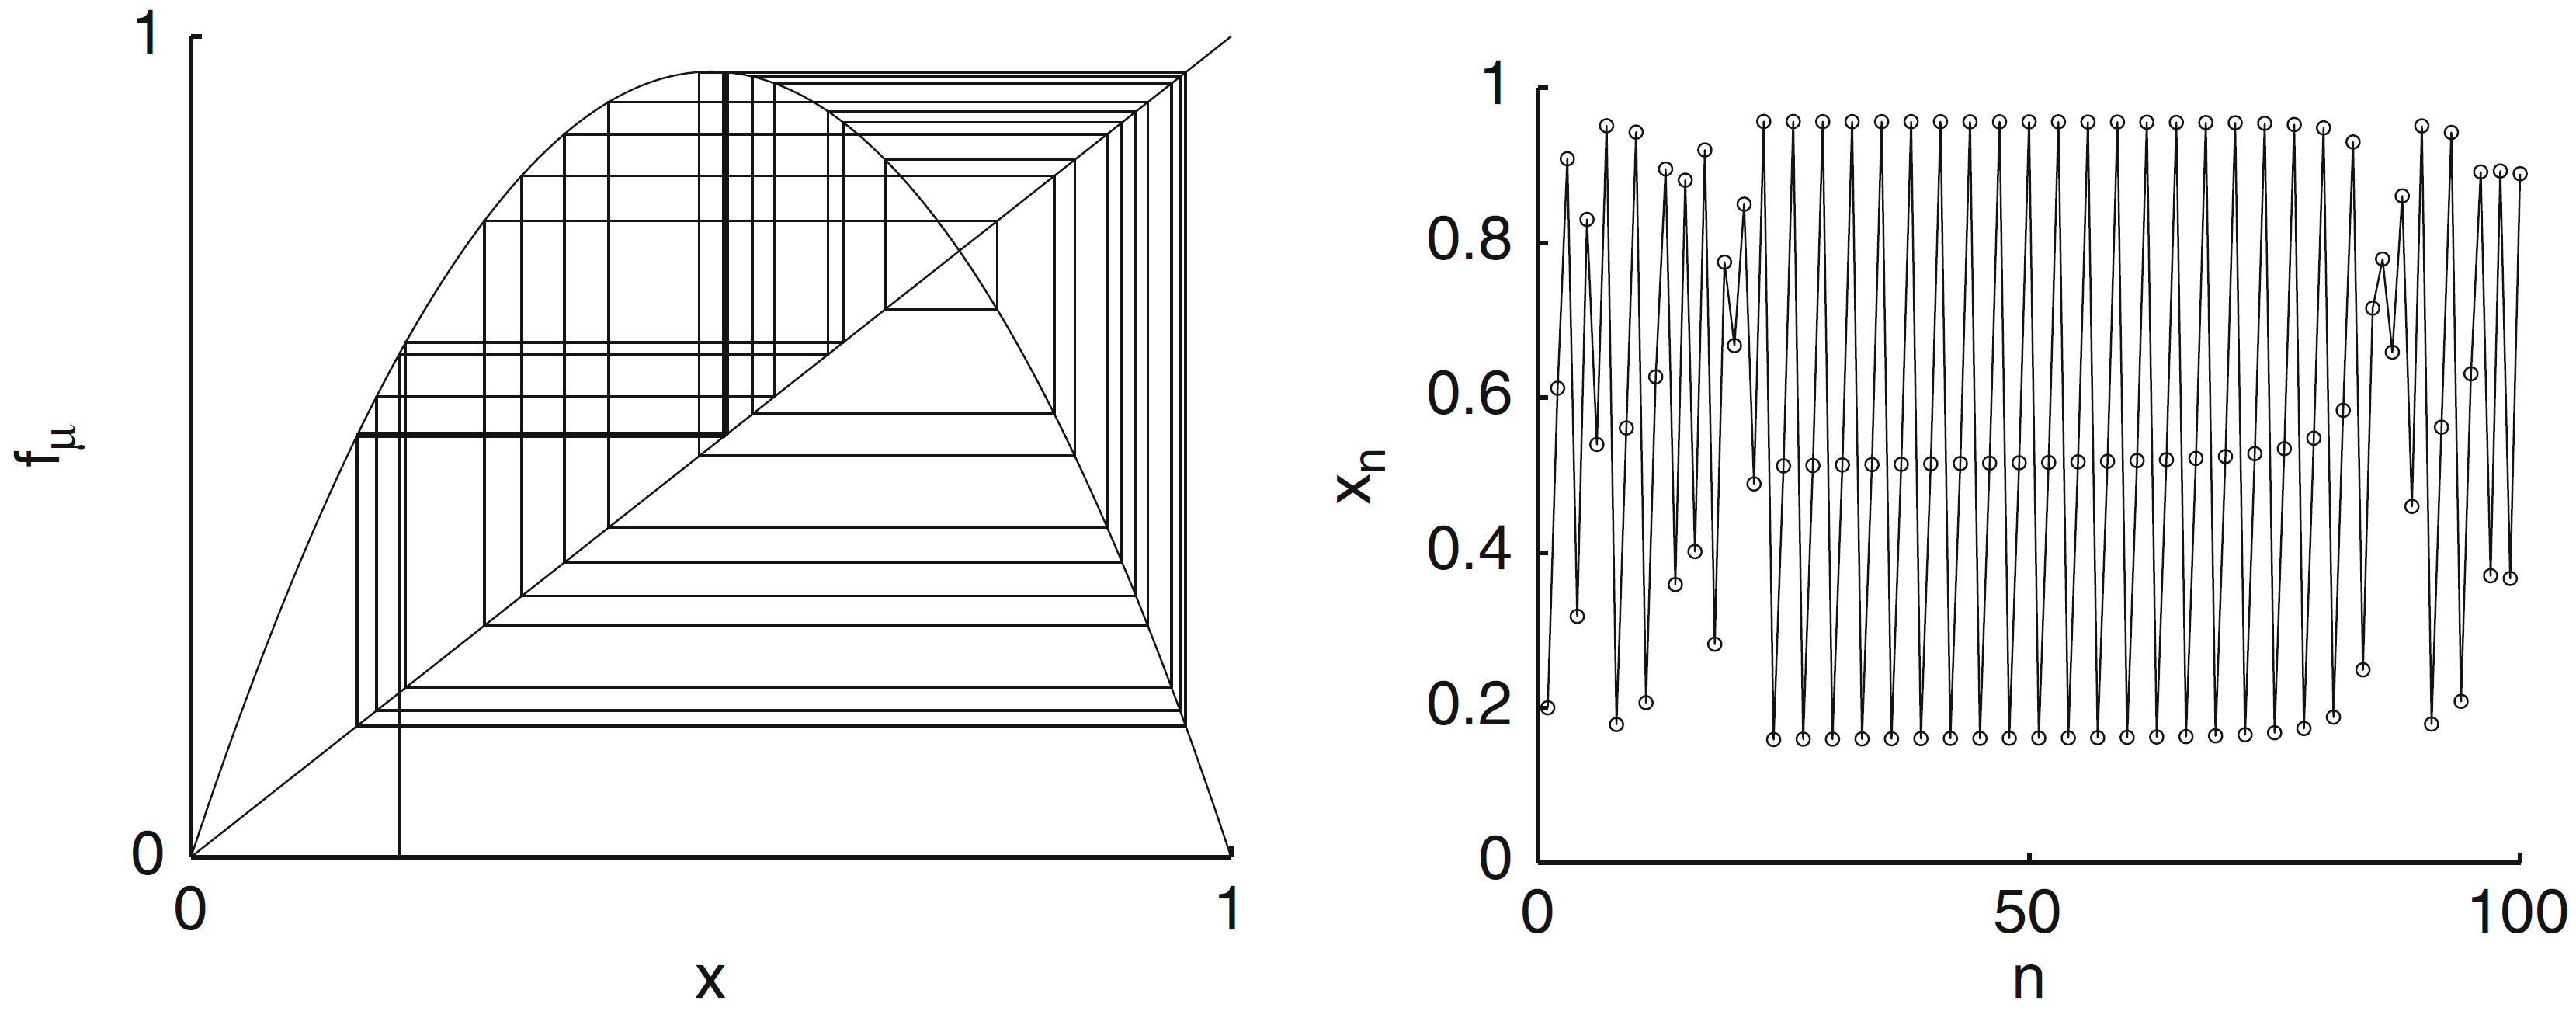
\includegraphics[width=0.5\linewidth]{itmrtc.png}
	\caption{Left: Iterative paths when $\mu=3.8282$ and $x_0=0.2$.\\Right: Time series data.}
	\label{fig:itmrtc}
\end{figure}
\begin{figure}[h!]
	\centering
	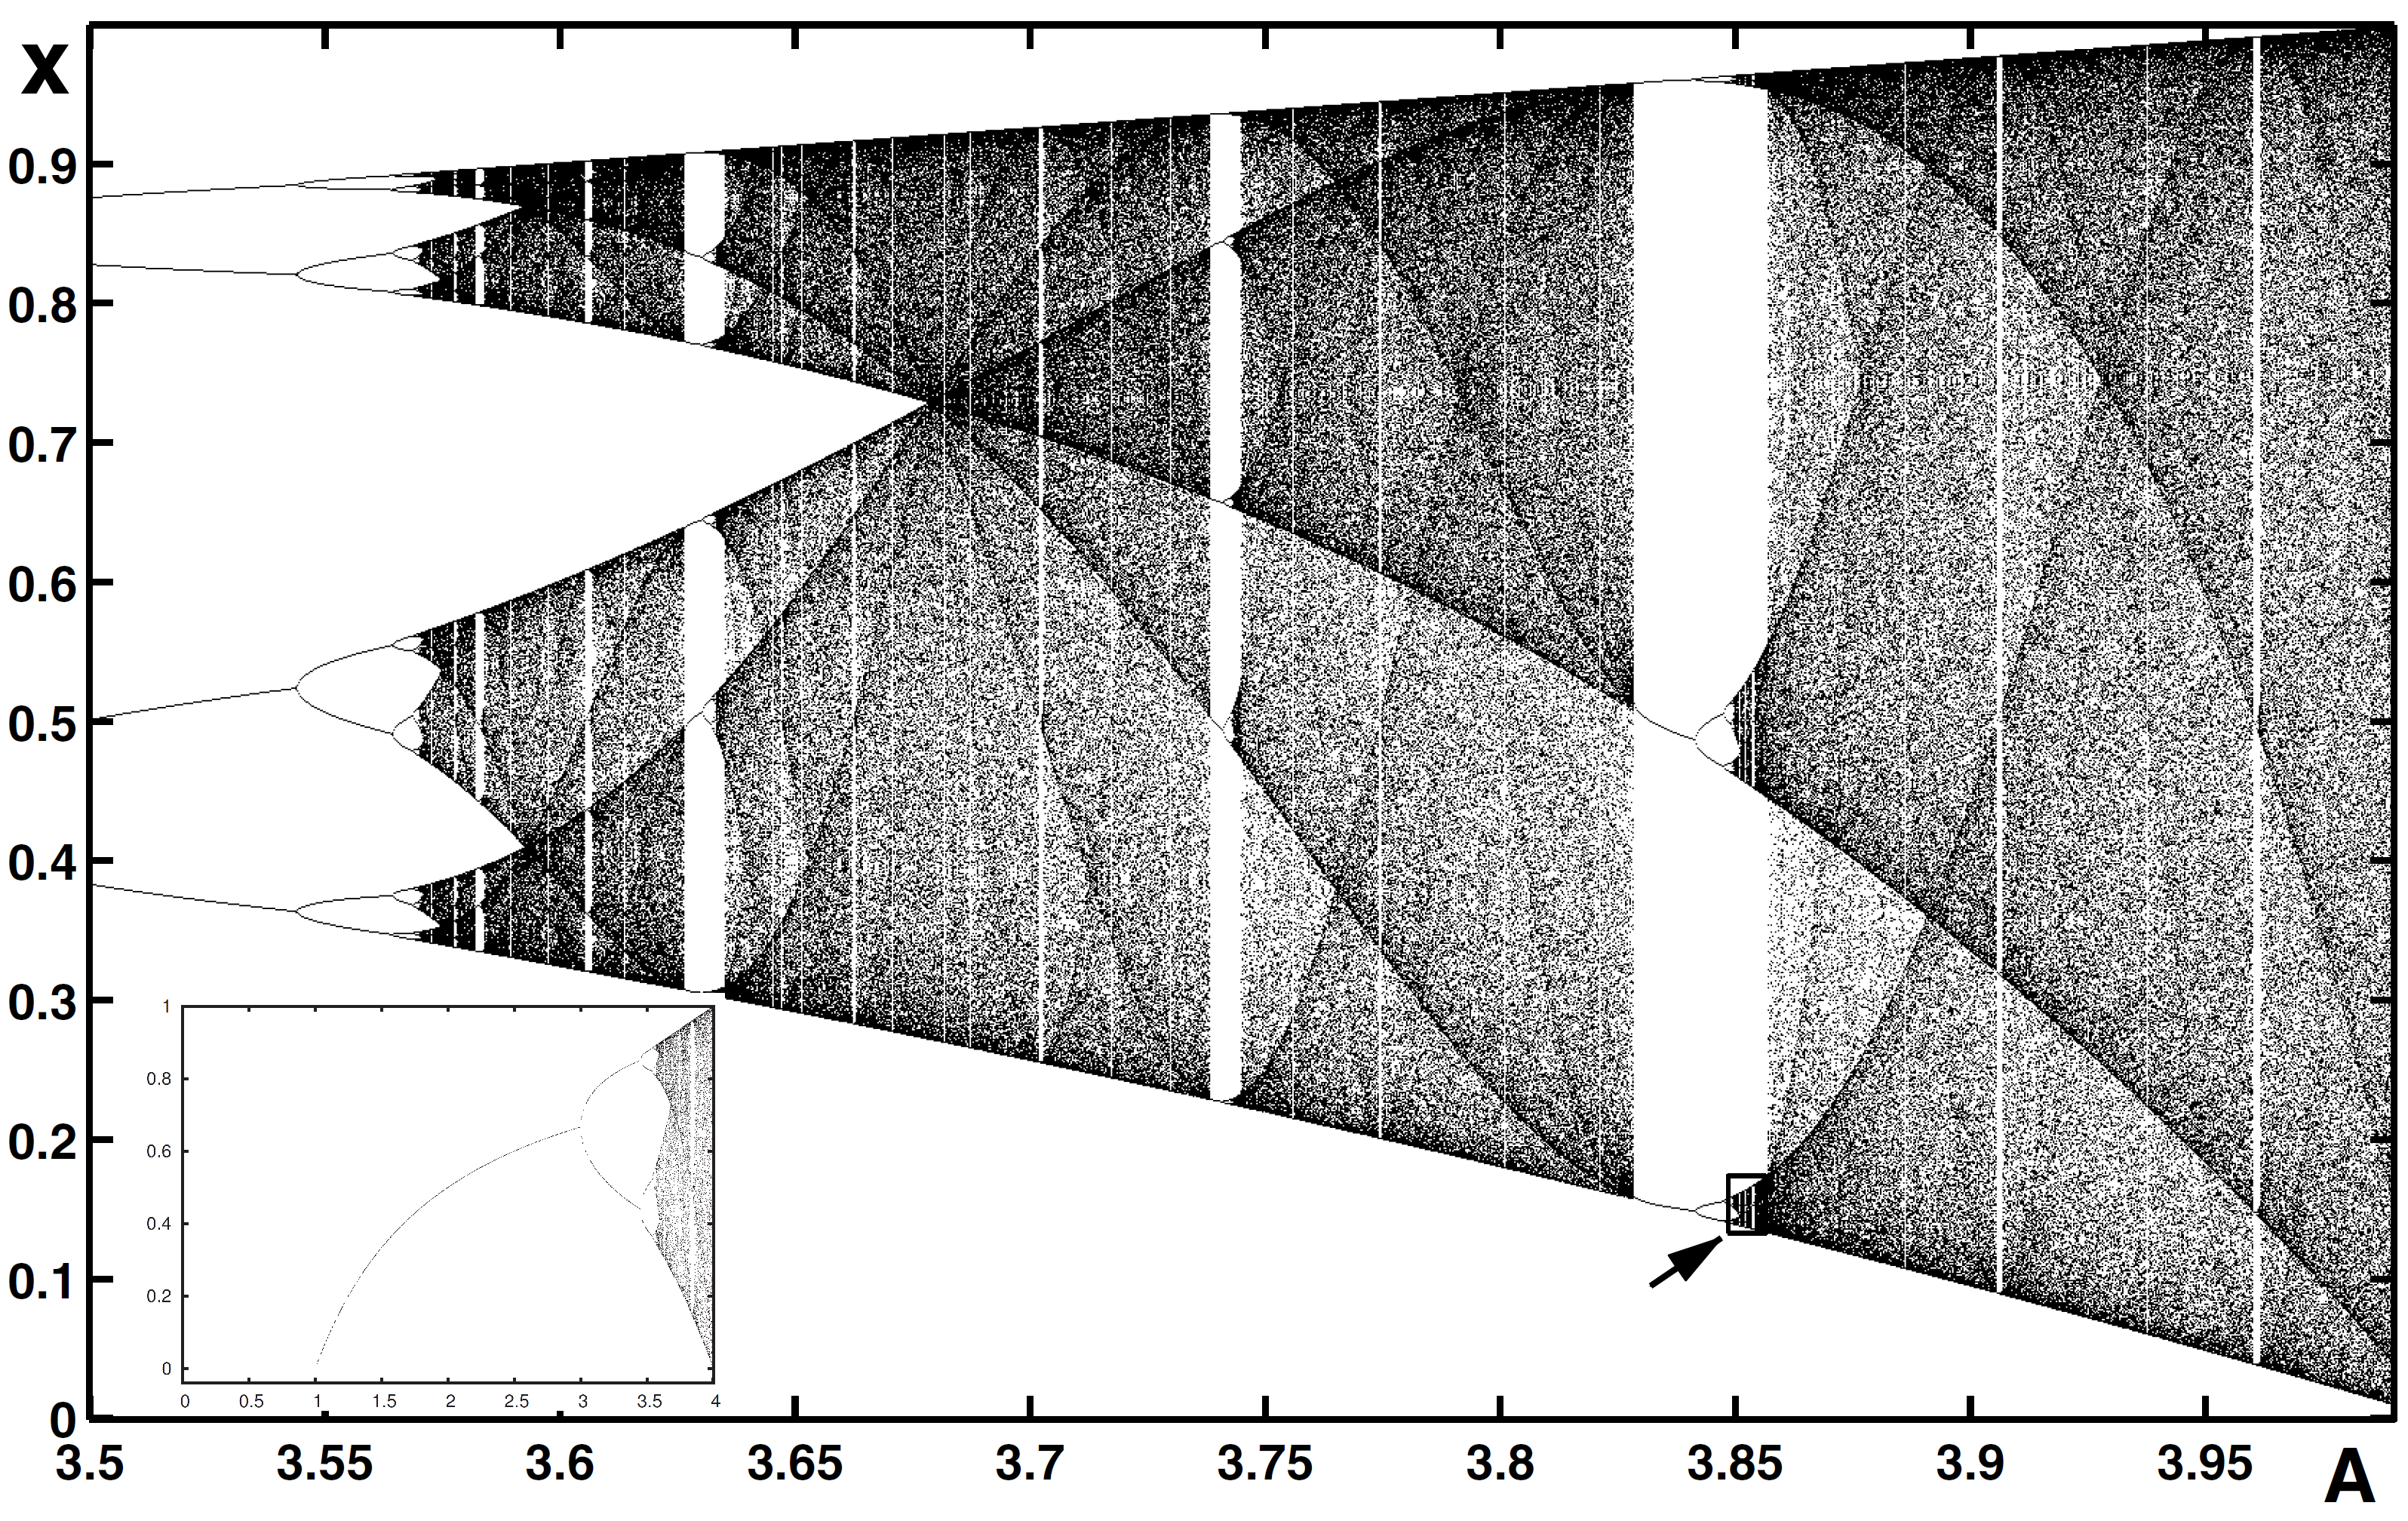
\includegraphics[width=0.7\linewidth]{lmbf.png}
	\caption{Bifurcation diagram for the logistic map for the ‘interesting’ range of the parameter $3.5\leq A\leq4$. The whole parameter range $0\leq A\leq4$ is shown in the insert.}
	\label{fig:lmbf}
\end{figure}
Near to the period-three window, the logistic map can display a new type of behavior known as \textbf{intermittency}, which is almost periodic behavior interrupted by occasional chaotic bursts.
A graphical iteration and time series plot are shown in Figure (\ref{fig:itmrtc}).
As the parameter $\mu$ is increased, the length of the intervals of chaotic bursts become larger and larger until the system becomes fully chaotic.
This phenomenon is known as an \textbf{intermittency route to chaos}.

\section{H\'enon Map}{\label{sec:hm}}
\input{Sections/Hénon Map}

\section{Universality}
\subsection{Bifurcation Diagrams for Other Functions}
\begin{figure}[h!]
	\centering
	\begin{subfigure}{0.45\linewidth}
		\centering
		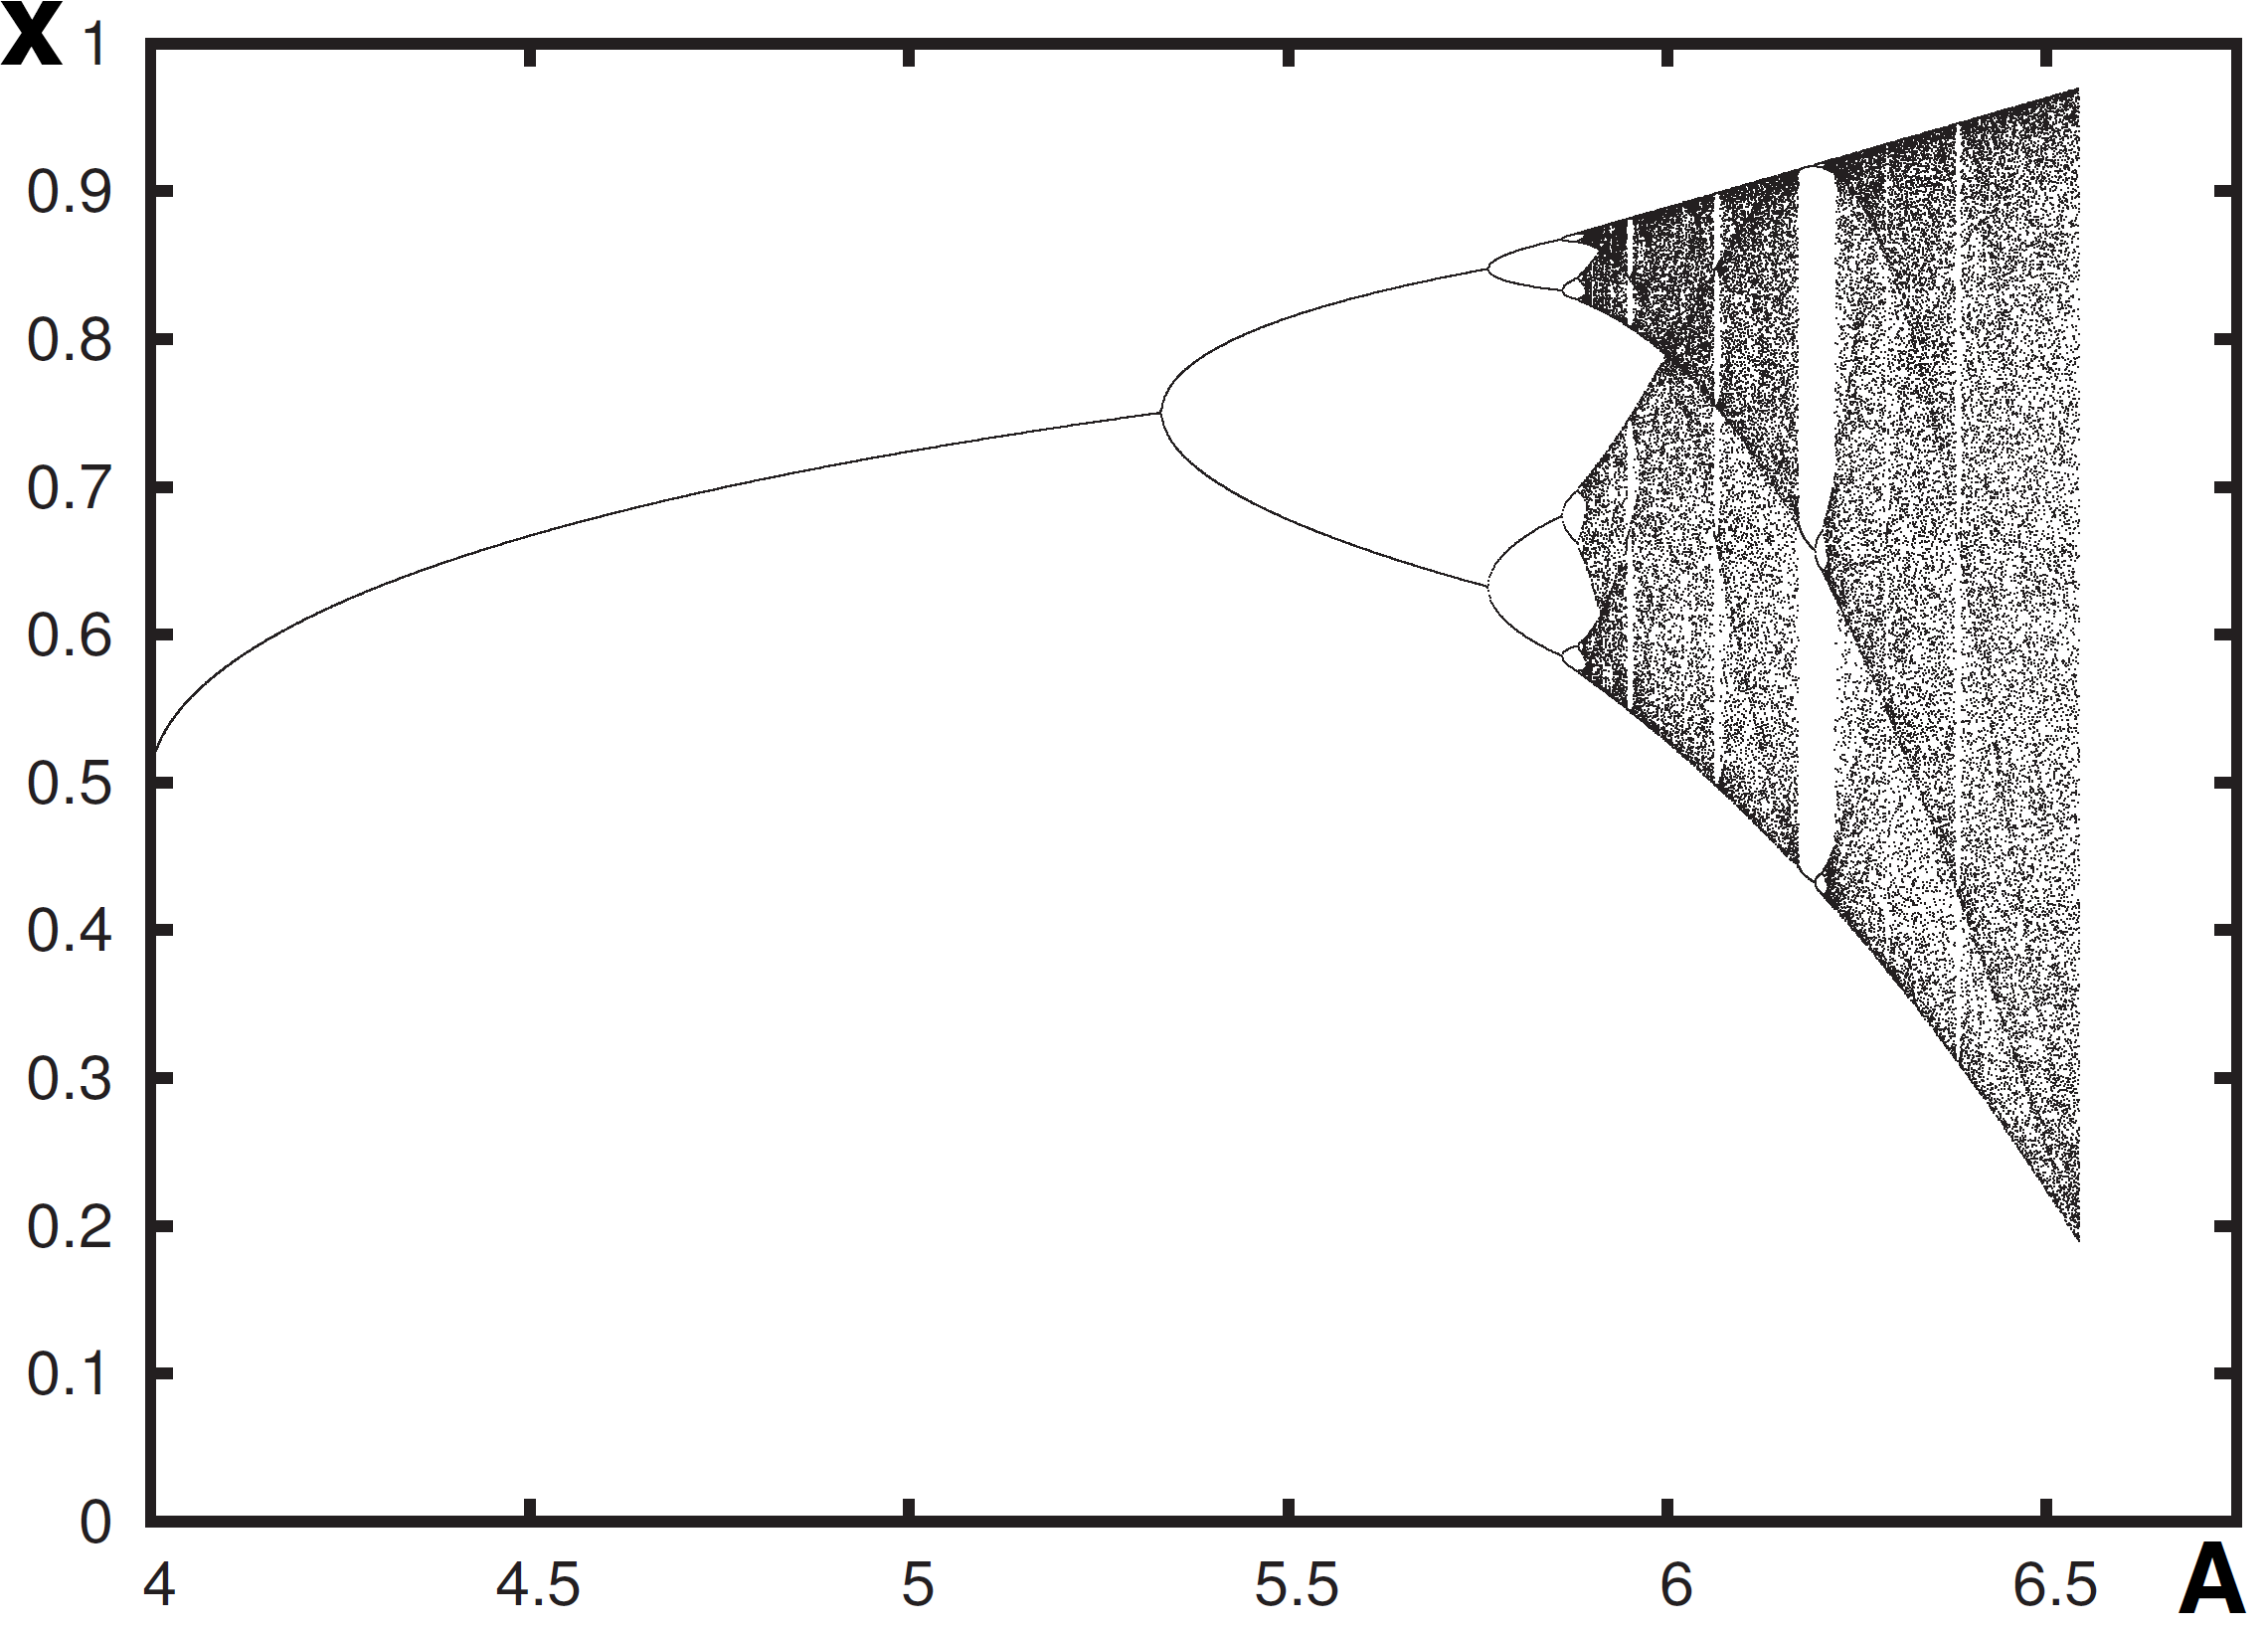
\includegraphics[width=\linewidth]{bfc.png}
		\caption{The bifurcation diagram for \\\centerline{$x_{n+1}=rx_n^2(1-x_n)$.}}
		\label{fig:bfc}
	\end{subfigure}
	\vline
	\begin{subfigure}{0.45\linewidth}
		\centering
		\includegraphics[width=\linewidth]{bfs.png}
		\caption{The bifurcation diagram for \\\centerline{$x_{n+1}=r\sin\left(\dfrac{\pi x_n}{2}\right)$.}}
		\label{fig:bfs}
	\end{subfigure}
	\caption{}
\end{figure}
Both systems given above has the \emph{same shape} as the graph of the logistic map.
Both curves are \emph{smooth}, \emph{concave} \emph{down}, and have a \emph{single} \emph{maximum}.
Such maps are called \textbf{unimodal}.
Both Bifurcations look similar.
In fact, we may at first think there has been some error and that logistic equation bifurcation diagram is accidentally used.
The \textbf{qualitative} dynamics of the two maps are identical.
They both undergo period-doubling routes to chaos, followed by periodic windows interwoven with chaotic bands.
\subsection{Qualitative Universality: U-Sequence}
The order in which stable periodic solutions appear is \emph{independent} of the unimodal map being iterated.
That is, the \emph{periodic} \emph{attractors} always occur in the \emph{same sequence}, now called the universal or \textbf{U-sequence}.
\subsection{Sharkovsky Ordering}
Consider the following ordering of natural numbers $a\prec b$ means $a$ comes before $b$
\begin{equation*}
	\begin{aligned}
		&1\prec2\prec2^2\prec2^3\prec\cdots\prec2^n\prec\cdots\prec7\cdot2^n\prec5\cdot2^n\prec3\cdot2^n\prec\cdots\prec7\cdot2\prec5\cdot2\prec3\cdot2\prec\cdots\prec7\prec5\prec3\\
		&\text{In general}\quad(1\prec2\prec2^2\prec\cdots\prec2^n\prec2^n\cdot k\prec\cdots\prec2^2\cdot k\prec2\cdot k\prec k)\quad\text{where $k$ are odd and decreasing}
	\end{aligned}
\end{equation*}
\begin{theorem}[\textbf{Sharkovsky Theorem}]
	If a continuous map of an interval into itself has a cycle of period $m$, then it has a cycle of any period $\tilde{m}\prec m$.
	Moreover, for any $m$ there exists a continuous map that has a cycle of period $m$ but does not have cycles of periods $\tilde{m},\ m\prec\tilde{m}$ .
\end{theorem}
The consequences of this amazing result are manifold:\\
If $f$ has a point of period 3, then $f$ has periodic points of any period.\\
If $f$ has a point of period $k\neq2^n$, then $f$ has infinitely many periodic points.

\section{Feigenbaum Constants}
The first seven bifurcation points of the Logistic Map computed numerically, are given by \\
$A_1=3, A_2=3.449490\ldots, A_3=3.544090\ldots, A_4=3.564407\ldots, A_5=3.568759\ldots,
A_6=3.569692\ldots,\text{ and}\\ \ A_7=3.569891{\ldots}$\\
Feigenbaum discovered that the ratio of the differences of the parameter values where bifurcations occur approaches a universal constant called $\delta$ when $n$ goes to infinity
\begin{equation}
	\delta=\lim_{n\rightarrow\infty}\frac{A_{n}-A_{n-1}}{A_{n+1}-A_n}=4.6692016\ldots
\end{equation}
\begin{wrapfigure}{r}{0.5\textwidth}
	\centering
	\includegraphics[width=\linewidth]{fca.png}
	\caption{Universal scaling in the horizontal and vertical direction of a period doubling sequence.}
	\label{fig:fca}
\end{wrapfigure}
The number $\delta$, known as the \emph{Feigenbaum constant}, is universal in the sense that it is the same number for a big class of nonlinear maps, differential equations$\ldots$
In addition to the scaling along the parameter axis there is a similar property for the variable $x$ along the vertical axis in a bifurcation diagram.\\
The width of the pitchfork at the \textbf{superstable orbits}\footnote{Superstable orbits are those for which the magnitude of the derivative of an iterate vanishes $|f^{(n)\prime}(x_0)|=0$. For the logistic map $f^\prime(x)=A(1-2x)$ and therefore $x=0.5$ is a superstable orbit. The Lyapunov exponent at such an orbit is $\lambda=-\infty$ (\ref{sec:ledds}).} converges towards another universal constant, known as the Feigenbaum constant $\alpha$.
\begin{equation}
	\alpha=\lim_{n\rightarrow\infty}\frac{d_{n+1}}{d_n}\approx-2.502907875
\end{equation}
As shown in Figure (\ref{fig:fca}) for the first four locations $d_{1-4}$, the pitchfork alternates between above and below the superstable orbit, leading to $d$ values alternating between positive and negative and as a consequence to a negative sign for the constant $\alpha$.

\section{Lyapunov Exponents for Discrete Systems}{\label{sec:ledds}}
Starting with two initial values of $x_0$ and $x_0+\delta_0$ we perform $n$ iterations of the map
\begin{equation}
	\begin{aligned}
		x_n&=f^{(n)}(x_0)\\
		x_n+\delta_n&=f^{(n)}(x_0+\delta_0)
	\end{aligned}\quad\rightarrow\quad
	\delta_n=f^{(n)}(x_0+\delta_0)-f^{(n)}(x_0)
\end{equation}
where $f^{(n)}$ in the $n^{th}$ iterate of $f$.
The Lyapunov exponent $\lambda$ is defined by
\begin{equation}
	|\delta_n|=|\delta_0|e^{n\lambda}\quad\rightarrow\quad
	\lambda=\frac{1}{n}\ln\left|\frac{\delta_n}{\delta_0}\right|\quad\rightarrow\quad\lambda=\frac{1}{n}\ln\left|\frac{f^{(n)}(x_0+\delta_0)-f^{(n)}(x_0)}{\delta_0}\right|
\end{equation}
which in the limit $\delta_0\rightarrow0$ can be written as
\begin{equation}
	\lambda=\frac{1}{n}\ln|f^{(n)\prime}(x_0)|\quad\text{using chain rule}\quad\lambda=\frac{1}{n}\ln\left|\prod_{i=0}^{n-1}f^\prime(x_i)\right|=\frac{1}{n}\sum_{i=0}^{n-1}\ln|f^\prime(x_i)|
\end{equation}

\newpage
\part{Chaos and Fractals}

\section{Chaos}
A dynamical system is chaotic if it possesses all of the following properties:
\begin{itemize}
	\item The dynamical rule is \textbf{deterministic}.
	\item The orbits are \textbf{aperiodic}.
	\item The orbits are \textbf{bounded}.
	\item The dynamical system has \textbf{sensitive dependence on initial conditions\footnote{A function $f$ has sensitive dependence on initial conditions if there is some number $\delta$ such that for any $x_0$ there is a $y_0$ that is not more that $\epsilon$ away from $x_0$, where the initial condition $y_0$ has the property that there is some integer $n$ such that, after $n$ iterates, the orbit of $y_0$ is more than $\delta$ away from the orbit of $x_0$. That is, $|x_n-y_n|>\delta$.}}.
\end{itemize}
We have already seen examples of Chaos Section ((\ref{sec:ls}),(\ref{sec:rs}),(\ref{sec:lm}),(\ref{sec:hm})).

\section{Fractals}
A \textbf{fractal} is an object that displays self-similarity under magnification and can be constructed using a simple motif (an image repeated on ever-reduced scales).\\
A \textbf{fractal} is an object that has noninteger fractal dimension (See Section \ref{sec:fd}).
\subsection{The Cantor Set}
\begin{wrapfigure}{r}{0.3\linewidth}
	\centering
	\includegraphics[width=\linewidth]{tcs.png}
	\caption{An early generation of the Cantor set.}
	\label{fig:tcs}
\end{wrapfigure}
It is constructed by removing the middle third of a line segment at each stage of construction.
Thus, at stage 0, there is one line segment of unit length.
At stage 1, the middle third is removed to leave two segments each of length $\frac{1}{3}$.
Continuing in this way, there will be $N=2^k$ segments each of length $l=3^{-k}$.\\
If this process is continued to infinity, then
\begin{equation}
	\lim_{k\rightarrow\infty}2^k=\infty\quad\text{and}\quad\lim_{k\rightarrow\infty}3^{-k}=0
\end{equation}
By using the\emph{ ternary number system}, it is possible to classify which points in the unit interval belong to the Cantor set and which do not.
The Cantor set can be identified by points whose ternary fractions consist of \emph{zeroes and twos} only.
\subsection{The Koch Curve}
It is constructed by replacing a unit line segment with a motif consisting of four line segments each of length $\dfrac{1}{3}$.
\begin{figure}[h!]
	\centering
	\includegraphics[width=\linewidth]{tkc.png}
	\caption{Construction of the Koch curve up to stage 5.}
	\label{fig:tkc}
\end{figure}
At the $k^{th}$ stage there are $N=4^k$ line segments each of length $l=3^{-k}$.
\begin{equation}
	\lim_{k\rightarrow\infty}4^k=\infty\quad\text{and}\quad\lim_{k\rightarrow\infty}3^{-k}=0
\end{equation}
So the mathematical Koch curve consists of a curve that is infinitely long.
\subsection{Fractal Dimension}{\label{sec:fd}}
The concept of dimensions is quite intuitive as long as the dimension is a nonnegative integer and smaller or equal to three.
For simple geometrical objects like fixed points, limit cycles or tori the dimension is obvious, they are zero-, one- and two dimensional, respectively.\\
But what is the dimension of lorenz attractor? Its trajectory stays within a finite volume, it is not closed (in which case it would be a limit cycle), it does not cover a surface entirely as the quasi-periodic systems, nor does it fill a volume.\\
There are several ways to generalize the idea.
\subsubsection{Hausdorff index}
A self-similar fractal has fractal dimension (or Hausdorff index) $D_f$ given by
\begin{equation}
	D_f=\frac{\ln N(l)}{-ln l}\quad\equiv\quad N(l)\propto(l)^{-D_f}
\end{equation}
where $l$ represents a scaling and $N(l)$ denotes the number of segments of length $l$. 
\subsubsection{Correlation dimension}
We randomly distribute points along an interval on a line and within a square as shown in Figure (\ref{fig:fdcd}).
\begin{figure}[h!]
	\centering
	\includegraphics[width=0.4\linewidth]{fdcd.png}
	\caption{Determining the dimension of a line and a plane}
	\label{fig:fdcd}
\end{figure}
Now we pick one of these points and count how many other points are located within a distance $\epsilon$.
It is intuitively clear that for the one-dimensional line this number $N(\epsilon)$ will be proportional to $\epsilon$, for the two-dimensional square it will be proportional to $\epsilon^2$.
In general, the number of points within a radius $\epsilon$ from a given point $\mathbf{x}$ is proportional to $\epsilon^d$ where $d$ is a generalized dimension, the so-called pointwise dimension of that point.
The correlation dimension for an attractor is found by calculating and averaging $N(\epsilon)$ for all points on the attractor and plotting $\log N(\epsilon)$ as a function of $\log\epsilon$.
\begin{equation}
	N(\epsilon)\sim\epsilon^d\quad\rightarrow\quad N(\epsilon)=c\epsilon^d\quad\rightarrow\quad\log N(\epsilon)=d\log\epsilon+\log c
\end{equation}
\subsubsection{Generalised Fractal Dimensions}
The generalized (box-counting) fractal dimensions $D_q$, where $q\in\mathbb{R}$, are defined by
\begin{equation}
	D_q=\lim_{l\rightarrow0}\frac{1}{1-q}\frac{\ln\sum\limits_{i=1}^Np_i^q(l)}{-\ln l}\quad\text{where}\quad p_i(l)=\frac{N_i(l)}{N}
\end{equation}
Where the index $i$ labels the individual boxes of size $l$ and $p_i(l)$ denotes the relative weight of the $i^{th}$ box or the probability of the object lying in the box.
$N_i(l)$ is the weight of the $i^{th}$ box and $N$ is the total weight of the object.
\begin{equation}
	D_0=D_f=\lim_{l\rightarrow0}\frac{\ln N(l)}{-\ln l}\quad
	D_1=\lim_{l\rightarrow0}\frac{\sum\limits_{i=1}^Np_i\ln(p_i)}{-\ln l}
\end{equation}
The quantity $D_0$ is known as the \textbf{hausdorff dimension}.
The quantity $D_1$ is known as the \textbf{information dimension}.
The quantity $D_2$ is known as the \textbf{correlation dimension} and indicates the correlation between pairs of points in each box.
The generalized dimensions $D_3,D_4,\ldots$ are associated with correlations between triples, quadruples, etc., of points in each box.
\subsection{Iterated Function Systems}
An iterated function system consists of several affine transformations which are applied in a random fashion, a procedure sometimes called the \textbf{chaos game}.\\
Affine transformations are linear transformations where a vector is rotated, scaled and shifted.
\begin{equation}
	\begin{pmatrix}
		x_{n+1}\\y_{n+1}
	\end{pmatrix}=
	\begin{pmatrix}
		a&b\\c&d
	\end{pmatrix}
	\begin{pmatrix}
		x_n\\y_n
	\end{pmatrix}+
	\begin{pmatrix}
		e\\f
	\end{pmatrix}\quad\equiv\quad
	\begin{pmatrix}
		x_{n+1}\\y_{n+1}\\1
	\end{pmatrix}=
	\begin{pmatrix}
		a&b&e\\c&d&f\\0&0&1
	\end{pmatrix}
	\begin{pmatrix}
		x_n\\y_n\\1
	\end{pmatrix}
\end{equation}
The rules of the chaos game can be generalized as follows:
\begin{itemize}
	\item Create two or more affine linear transformations.
	\item Assign probabilities to each of the transformations.
	\item Start with an initial point.
	\item Select a random transformation to get a second point.
	\item Repeat the process.
\end{itemize}
\begin{figure}[h!]
	\centering
	\begin{subfigure}{0.45\linewidth}
		\centering
		\includegraphics[width=\linewidth]{ifssg.png}
		\caption{The Sierpinsky triangle or gasket}
		\label{fig:ifssg}
	\end{subfigure}
	\vline
	\begin{subfigure}{0.4\linewidth}
		\centering
		\includegraphics[width=\linewidth]{ifsbf.png}
		\caption{Barnsley’s fractal fern}
		\label{fig:ifsbf}
	\end{subfigure}
	\caption{}
\end{figure}
\begin{figure}[h!]
	\centering
	\begin{subfigure}{0.35\linewidth}
		\centering
		\includegraphics[width=\linewidth]{ifssgat.png}
		\caption{The regions that get covered when the transformations $t_1-t_3$ are applied.}
		\label{fig:ifssgat}
	\end{subfigure}
	\vline
	\begin{subfigure}{0.45\linewidth}
		\centering
		\includegraphics[width=\linewidth]{ifsbfat.png}
		\caption{The regions that get covered when the transformations $t_1-t_4$ are applied.}
		\label{fig:ifsbfat}
	\end{subfigure}
	\caption{}
\end{figure}
\subsubsection{Sierpinsky gasket}
This structure is constructed geometrically by starting with a solid black triangle and removing the large white triangle in the middle which leaves three black triangles after the first iteration step.
Then this procedure is applied to each of these triangles leading to nine smaller ones and so on.
{\renewcommand{\arraystretch}{1.2}
\begin{table}[h!]
	\centering
	\caption{Parameters for Iterated Function Systems}
	\label{tab:ifs}
	\subfloat[Sierpinski gasket]{
	\begin{tabular}{c c c c c c c c}
		&a&b&c&d&e&f&p\\
		\hline
		$t_1$&0.5&0&0&0.5&0&0&1/3\\
		$t_2$&0.5&0&0&0.5&0.5&0.5&1/3\\
		$t_3$&0.5&0&0&0.5&0.5&0&1/3\\
	\end{tabular}
	}
	\quad\vline\quad
	\subfloat[Barnsley’s fractal fern]{
	\begin{tabular}{c c c c c c c c}
		&a&b&c&d&e&f&p\\
		\hline
		$t_1$&0&0&0&0.16&0&0&0.01\\
		$t_2$&0.2&$-$0.26&0.23&0.22&0&1.6&0.07\\
		$t_3$&$-$0.15&0.28&0.26&0.24&0&0.44&0.07\\
		$t_4$&0.85&0.04&$-$0.04&0.85&0&1.6&0.85\\
	\end{tabular}
	}
\end{table}}
\\The parameters for the three transformations that are used to create the Sierpinski gasket by an iterated function system are shown in Table (\ref{tab:ifs}a).
There is an additional column listing a parameter $p$, which is the probability that this particular transformation is applied.
Figure (\ref{fig:ifssgat}) are three plots showing the points of Figure (\ref{fig:ifssg}) that arise after the transformations $t_1$, $t_2$ and $t_3$ are executed.
In the case of the Sierpinski gasket they fall into the three triangular regions that remain after the big triangle in the middle is removed.
\subsubsection{Barnsley’s Fern}
The Fractal Fern shown in Figure (\ref{fig:ifsbf}) together with smaller plots of the regions that are created by using only the points after a particular transformation has been applied.\\\\
The basic idea of \textbf{fractal compression of images} is that if pictures of natural scenes (like a fern) are encoded as pixels, a high resolution is necessary to preserve the complex structure, resulting in a huge amount of bits that have to be stored.
In contrast, for the fern for instance, only $4\cdot7=28$ numbers are needed and the image can be restored at any desired resolution.\\
The problem is that even though there were attempts to develop algorithms for finding the transformations and parameters for encoding a general image, the most impressive examples of fractal compression still need human intervention.
\subsection{Complex Iterative Maps}
\subsubsection{Julia Sets}
Consider a complex polynomial mapping of the form $z_{n+1}=f(z_n)$.
The points that lie on the boundary between points that orbit under $f$ and are bounded and those that orbit under $f$ and are unbounded are collectively referred to as the \textbf{Julia set}.\\
Consider the quadratic map
\begin{equation}
	z_{n+1}=f_c(z_n)=z_n^2+c\quad\text{where}\quad z_n,c\in\mathbb{C}
\end{equation}
The following are properties of a Julia set, say, $J$
\begin{itemize}
	\item The set $J$ is a \textbf{repellor}. 
	\item The set $J$ is \textbf{invariant}. 
	\item An orbit on $J$ is either \textbf{periodic} or \textbf{chaotic}. 
	\item All \textbf{unstable periodic} points are on $J$. 
	\item The set $J$ is either \textbf{wholly} \textbf{connected} or \textbf{wholly} \textbf{disconnected}. 
	\item The set $J$ nearly always has \textbf{fractal} structure.
\end{itemize}
\begin{figure}[h!]
	\centering
	\includegraphics[width=\linewidth]{js.png}
	\caption{Julia sets for $c=0,-0.72i,-0.1-0.88i,-0.6+0.2i,-0.6+0.45i,0.37+0.37i,-0.25-0.7i$}
	\label{fig:js}
\end{figure}
\subsubsection{The Mandelbrot Set}
The Mandelbrot Set is the collection of $c$ values for which the \textbf{Julia sets are connected}.\\\\
There is an efficient way to determine the Mandelbrot Set as follows:\\
If the orbit of $z_0=0$ for $f(z)=z^2+c$ is \textbf{bounded}, then $c$ is in the Mandelbrot set.\\
If the orbit is \textbf{not} \textbf{bounded}, then $c$ is not in the Mandelbrot set.
\begin{figure}[h!]
	\centering
	\begin{subfigure}{0.45\linewidth}
		\centering
		\includegraphics[width=\linewidth]{ms1.jpg}
		\caption{The Mandelbrot Set complete}
		\label{fig:ms1}
	\end{subfigure}
	\begin{subfigure}{0.45\linewidth}
		\centering
		\includegraphics[width=\linewidth]{ms2.jpg}
		\caption{Seahorse Valley}
		\label{fig:ms2}
	\end{subfigure}
	\begin{subfigure}{0.45\linewidth}
		\centering
		\includegraphics[width=\linewidth]{ms3.jpg}
		\caption{Seahorse Valley Zoom}
		\label{fig:ms3}
	\end{subfigure}
	\begin{subfigure}{0.45\linewidth}
		\centering
		\includegraphics[width=\linewidth]{ms4.jpg}
		\caption{Seahorse}
		\label{fig:ms4}
	\end{subfigure}
	\caption{}
	\label{fig:ms}
\end{figure}
\subsubsection*{Boundaries of Periodic Orbits}
The fixed points of period one are given by
\begin{equation}
	z=z^2+c=f_c(z)\quad\rightarrow\quad z_{1,1}=\frac{1+\sqrt{1-4c}}{2}\qquad z_{1,2}=\frac{1-\sqrt{1-4c}}{2}
\end{equation}
where $z_{m,n}$ is the $n^{th}$ fixed point of period $m$.
For stability,
\begin{equation}
\frac{df_c}{dz}=2z=re^{i\theta}\quad\text{where}\quad r\geq0\quad0\leq\theta<2\pi\quad\rightarrow\quad c=\frac{re^{i\theta}}{2}-\frac{r^2e^{i2\theta}}{4}
\end{equation}
The boundary of points of period one is given by
\begin{equation}
	\left|\frac{df_c}{dz}(z_{1,1})\right|=|2z_{1,1}|=r=1
\end{equation}
\begin{equation}
	\text{Let}\ c=x+iy\quad\rightarrow\quad x=\frac{1}{2}\cos\theta-\frac{1}{4}\cos(2\theta)\qquad y=\frac{1}{2}\sin\theta-\frac{1}{4}\sin(2\theta)
\end{equation}
The parametric curve is plotted in Figure (\ref{fig:bpoms}) and forms a \textbf{cardioid} that lies at the heart of the Mandelbrot set.
\begin{wrapfigure}{r}{0.3\linewidth}
	\centering
	\includegraphics[width=\linewidth]{bpoms.png}
	\caption{The boundary of fixed points of periods one and two for the Mandelbrot set.}
	\label{fig:bpoms}
\end{wrapfigure}
Using similar arguments to those above, it is not difficult to extend the analysis to determine the boundary for the fixed points of period two.
\begin{equation}{\label{eq:p2ms1}}
	f_c^2(z)=(z^2+c)^2+c=z\quad\rightarrow\quad
	\begin{aligned}
		z^4+2cz^2-z+c^2+c&=0\\
		(z^2-z+c)(z^2+z+c+1)&=0
	\end{aligned}
\end{equation}
$z_{1,1}$ and $z_{1,2}$ satisfy equation (\ref{eq:p2ms1}).
\begin{equation*}
	z^2+z+c+1=0\quad\rightarrow\quad z_{2,1}=\frac{-1+\sqrt{-3-4c}}{2}\qquad z_{2,2}=\frac{-1-\sqrt{-3-4c}}{2}
\end{equation*}
The stability of each critical point is determined from the derivative of the map at the point
\begin{equation*}
	\frac{df_c^2}{dz}=4z(z^2+c)\quad\rightarrow\quad\left|\frac{df_c^2}{dz}(z_{2,1})\right|=|4+4c|\quad\text{the boundary is given by}\quad|c+1|=\frac{1}{4}
\end{equation*}
The parametric curve is plotted in Figure (\ref{fig:bpoms}) and forms a \textbf{circle} centered at $(-1,0)$ of radius $\dfrac{1}{4}$ in the Argand plane.
\subsubsection{The Newton Fractal}
The Newton-Raphson method, can be used to find the roots of the equation $f(z)=0$ using the iterative formula
\begin{equation}
	z_{n+1}=z_n-\frac{f(z_n)}{f^\prime(z_n)}
\end{equation}
\begin{figure}[H]
	\centering
	\includegraphics[width=0.6\linewidth]{nf.png}
	\caption{Julia sets for the rational function associated with Newton’s method for $f(z)=z^3-1$}
	\label{fig:nf}
\end{figure}
A Newton fractal is the Julia set of $f(z_n)$ and shows that the numerical method can be very sensitive to its choice of initial starting point.\\
In Figure (\ref{fig:nf}),
\begin{itemize}
	\item All points in the red regions are in the basin of attraction for the fixed point at $\tilde{z}_1=1$.
	\item All points in the green regions are in the basin of attraction for the fixed point at $\tilde{z}_2=\dfrac{-1+\sqrt{3}i}{2}$.
	\item And all points in the blue regions are in the basin of attraction for the fixed point at $\tilde{z}_3=\dfrac{-1-\sqrt{3}i}{2}$.
\end{itemize}
The boundary between the different basins of attraction forms a Julia set.
{\let\thefootnote\relax\footnote{{The colors in Figure (\ref{fig:ms}) are determined by the number of iterations the points take to go out of bounding region}.}}

\newpage
\part{Stochastic Systems}
So far we have dealt with systems that are purely \emph{deterministic}, which means that for two identical systems with \emph{exactly} the same initial conditions, their trajectories will be the same for all times.
However, for the case of deterministic chaos, a tiny difference in the initial condition can lead to a completely different \emph{long-term behavior}. In contrast to deterministic systems, for stochastic systems not even the \emph{short-term behavior} is predictable, not even in principle, because there are forces at work that are outside of our control.\\
All relevant systems in nature contain both deterministic and stochastic elements, and the question is simply which part, if any, is \emph{dominating}.\\
If there were no random forces, effects like the \emph{spontaneous breaking of symmetry} discussed in section (\ref{sec:spcpbf}) could not occur.
If a potential landscape switches from a single minimum to a double-well as in Figure (\ref{fig:spbf}), nothing would happen, the system would simply sit at the unstable fixed point until someone comes along and kicks it a little.\\
The \textbf{stochastic force} allows the system to explore all of its phase space as we shall see.
Without such a force the system is restricted to a single trajectory from an initial condition to an attractor or to infinity, or is even left stranded at an unstable equilibrium point.

\section{Langevin Equations}
\subsection{Brownian Motion}
The field of stochastic systems started with an observation by Robert Brown in 1827.
In Brown’s experiment, there are two types of forces at work.\\
First, even with the particle at rest, it is bombarded by gas or fluid molecules in its surrounding.\\
Secondly, if the particle is moving, it will face more energetic collisions in the direction it is moving, and the particle will slow down.\\
This process is described at the macroscopic level by the frictional force which is exerted on a particle in a viscous fluid and leads to an acceleration opposite to the direction of its velocity.
Assuming the particle is spherical this force is given by Stoke’s law as
\begin{equation}
	\mathbf{F}=-6\pi\eta R\mathbf{v}
\end{equation}
where $\eta$ is the viscosity of the fluid and $R$ the radius of the sphere.\\
Regarding the process that leads to the movement, we have no idea what force is acting on the particle at a given time, neither its strength, nor its direction, so we simply call it $\mathbf{\tilde{\xi}}(t)$.\\
For simplicity we look at at a one-dimensional system, i.e. a particle that only moves along a line to the left or right. Then Newton’s second law can be applied:
\begin{equation}{\label{eq:bm1}}
	F=ma=-6\pi\eta rv+\tilde{\xi}(t)\quad\rightarrow\quad a=\dot{v}=-\underbrace{\frac{6\pi\eta R}{m}}_{\alpha}v+\underbrace{\frac{1}{m}\tilde{\xi}(t)}_{\xi(t)}
\end{equation}
Inserting the substitutions as indicated in (\ref{eq:bm1}) we obtain
\begin{equation}{\label{eq:bm2}}
	\dot{v}=-\alpha v+\xi(t)
\end{equation}
Equations of the form (\ref{eq:bm2}) with a deterministic part (here $-\alpha v$) and an additive stochastic part (here $\xi(t)$) are called \textbf{Langevin equations}.\\
We have always dealt with equations that are called \emph{autonomous} or \emph{homogeneous}, which means that the right-hand side does not explicitly depend on time.
Equations like (\ref{eq:bm2}) that contain such an explicit time dependence are called \emph{nonautonomous} or \emph{inhomogenous}.
\begin{theorem}
	The general solution of an \emph{inhomogeneous} differential equation is given by the the \emph{sum} of the general solution of the corresponding homogenous equation and a particular solution of the inhomogeneous equation.
\end{theorem}
According to this theorem we first have to find the general solution of the homogeneous equation,
\begin{equation}
	\dot{v}=-\alpha v\quad\rightarrow\quad v(t)=ce^{-\alpha t}
\end{equation}
Now we have to find a particular solution of the inhomogenous equation, which is done by a procedure called \emph{variation of the constant}.
The constant $c=c(t)$
\begin{equation}
	v_p(t)=c(t)e^{-\alpha t}\quad\rightarrow\quad \dot{v}_p(t)=\dot{c}(t)e^{-\alpha t}-\alpha c(t)e^{-\alpha t}
\end{equation}
which we insert into the original equation (\ref{eq:bm2}) to determine the ‘constant’ $c(t)$
\begin{equation}
	\dot{v}_p(t)=\dot{c}(t)e^{-\alpha t}-\alpha c(t)e^{-\alpha t}=-\alpha c(t)e^{-\alpha t}+\xi(t)\quad\rightarrow\quad \dot{c}(t)=\xi(t)e^{\alpha t}\quad\rightarrow\quad c(t)=\int_{-\infty}^t\xi(t^\prime)e^{\alpha t^\prime}dt^\prime
\end{equation}
Now the particular solution of the inhomogeneous equation reads
\begin{equation}{\label{eq:lesn}}
	v_p(t)=e^{-\alpha t}\int_{-\infty}^t\xi(t^\prime)e^{\alpha t^\prime}dt^\prime\quad\rightarrow\quad v(t)=ce^{-\alpha t}+e^{-\alpha t}\int_{-\infty}^t\xi(t^\prime)e^{\alpha t^\prime}dt^\prime
\end{equation}
For large $t$ the first term in (\ref{eq:lesn}) vanishes and we finally obtain
\begin{equation}{\label{eq:lesln}}
	v(t)=\int_{-\infty}^t\xi(t^\prime)e^{-\alpha(t-t^\prime)}dt^\prime
\end{equation}
\begin{figure}[H]
	\centering
	\begin{subfigure}{0.55\linewidth}
		\centering
		\includegraphics[width=\linewidth]{rss.png}
		\caption{Two realizations calculated from (\ref{eq:lesln})}
		\label{fig:rss}
	\end{subfigure}
	\vline
	\begin{subfigure}{0.35\linewidth}
		\centering
		\includegraphics[width=\linewidth]{tspspss.png}
		\caption{Time series and phase space plot for a solution of (\ref{eq:bm2}).}
		\label{fig:tspspss}
	\end{subfigure}
\end{figure}
Two time series calculated from (\ref{eq:lesln}) are shown in Figure (\ref{fig:rss}), where the values for $\xi(t)$ were obtained from a random number generator.
Such different solutions of (\ref{eq:bm2}) are called \textbf{realizations} of the stochastic system.\\ Evidently, the time series are quite different, however the \emph{distributions} of the values in the time series, represented by the histograms, are very similar.
Such distributions are the foundation of stochastic systems.\\
In Figure (\ref{fig:tspspss}), without the stochastic term the trajectory would evolve to the stable fixed point $\tilde{v}=0$ but the stochastic force allows the system to explore its \emph{entire phase space}.
In contrast to deterministic systems, the trajectories in stochastic systems \emph{intersect}.

\section{Features}
\subsection{Averages}
If we could deal with time series of infinite length, the distributions for a given system would be exactly the same.
This leads to the conclusion that other quantities like mean values or averages are more appropriate to describe the properties of such systems than their time series.
\paragraph{Time Average}
It is usually denoted by a bar $\bar{\ldots}$ over the quantity to be
averaged and calculated simply as the mean of a time series
\begin{equation}
	\bar{q}=\frac{1}{T}\int_0^T q(t)dt
\end{equation}
\paragraph{Ensemble Average}
It is usually denoted by brackets $\langle \ldots\rangle$ around the quantity, is calculated as the mean of the values from different realizations $k$ at the same point in time
\begin{equation}
	\langle q(t)\rangle=\frac{1}{N}\sum_{k=1}^N q_k(t)
\end{equation}
For so-called \textbf{Ergodic Systems\footnote{Ergodicity is a complicated matter. Roughly, a system is ergodic when its trajectory comes infinitely close to every point in phase space compatible with the system’s energy. All system we are talking about here are ergodic.}} the time and the ensemble average is the same $\bar{q}=\langle q(t)\rangle$.
Evidently, in this case the ensemble average is the same for all points in time.
\subsection{Distributions}
One of the main characteristics of a stochastic system is its \emph{probability distribution}.
The most common distribution, which is implemented in random number generators, is the \textbf{rectangular distribution}, where real numbers between 0 and 1 are drawn, all with the \emph{same probability}.
\subsubsection{Gaussian distribution}
It is given by
\begin{equation}
	g(x)=\frac{1}{\sigma\sqrt{2\pi}}e^{-\dfrac{(x-\mu)^2}{2\sigma^2}}\quad\text{with}\quad\int_{-\infty}^\infty g(x)\mathop{dx}=1
\end{equation}
where $\mu$ is the \emph{mean} and $\sigma$ the \emph{standard deviation}.
\paragraph{Properties of the Gaussian Distribution}
\begin{itemize}
	\item In very many cases the distributions found in nature are approximately Gaussian;
	\item It is a nontrivial distribution for which analytical results can be obtained.
\end{itemize}
The main reason for the first is that the sum of many independent stochastic variables has a Gaussian distribution whatever the individual distributions are.
More precisely, if the numbers $x_k$ are from independent stochastic processes then the variable
\begin{equation}
S_n=x_1+x_2+x_3+\cdots+x_n
\end{equation}
has a Gaussian distribution if $n$ goes to infinity independent of the distributions of the individual variables. This is the essence of the \textbf{central limit theorem}.\\
The second point has to do with a special property of the Gauss-function and what is known as the \emph{moments of a distribution}.
The $n_{th}$ moment $q(n)$ of a distribution $f(q)$ is define as
\begin{equation}
	q^{(n)}=\int_{-\infty}^\infty q^n f(q)\mathop{dq}
\end{equation}
This may look a little complicated but it is simply an extension of elementary statistics: the zeroth moment of any properly normalized distribution is 1 because it is just the integral over the distribution itself and the first moment is the mean value
\begin{equation}
	q^{(0)}=\int_{-\infty}^\infty f(q)\mathop{dq}=1\qquad q^{(1)}=\int_{-\infty}^\infty qf(q)\mathop{dq}=\langle q\rangle
\end{equation}
For $n>1$ it is more convenient to use the \emph{central moments} defined as
\begin{equation}
	\mu^{(n)}=\int_{-\infty}^\infty (q-\langle q\rangle)^n f(q)\mathop{dq}
\end{equation}
because the second central moment is the \emph{variance} with its square root the \emph{standard deviation}.
The third central moment defines the \emph{skewness} and the fourth the \emph{kurtosis} and so on.
\subsection{Correlations}
Besides distributions the second important property of a stochastic system is how fast (on average) it ‘forgets’ about its past, more precisely, how fast the \emph{correlations} within its time series decay.
A quantitative measure of correlation is the \emph{autocorrelation function}.\\
Imagine a time series $q(t)$ and a second time series, which is the same as the first, just shifted by a time $\tau$, $q(t-\tau)$, the autocorrelation function is defined as
\begin{equation}
	G(\tau)=\lim_{T\rightarrow\infty}\frac{\int\limits_{-T}^T q(t-\tau)q(t)\mathop{dt}}{\int\limits_{-T}^T q^2(t)\mathop{dt}}
\end{equation}
There exists an important relation between the autocorrelation function $G(\tau)$ of a time series and its spectrum $S(\omega)$, known as the \textbf{Wiener-Khinchin theorem}.
It states that the spectrum of a time series $S(\omega)$ is the Fourier transform of the autocorrelation function $G(\tau)$ and the autocorrelation function is the inverse Fourier transform of the spectrum.
We now have a look at the spectra and autocorrelation functions for three important cases.
\subsubsection{Periodic Signal}
Figure (\ref{fig:psas}) shows the time series $q(t)$ (a cosine), its distribution $p(q)$ and spectrum $S(\omega)$.
\begin{figure}[H]
	\centering
	\begin{subfigure}{0.45\linewidth}
		\centering
		\includegraphics[width=\linewidth]{psas.png}
		\caption{Properties of a periodic signal.}
		\label{fig:psas}
	\end{subfigure}
	\vline
	\begin{subfigure}{0.45\linewidth}
		\centering
		\includegraphics[width=\linewidth]{ucwnas.png}
		\caption{Properties of uncorrelated noise.}
		\label{fig:ucwnas}
	\end{subfigure}
	\caption{Left: Time series; middle: probability distribution; right: spectrum.}
\end{figure}
it can be shown that the distribution for the cosine function
\begin{equation}
	q(t)=\cos\Omega t\quad\text{is given by}\quad p(q)=\frac{1}{\sin\{\cosi q\}}
\end{equation}
We now calculate the autocorrelation function
\begin{equation}
	\begin{aligned}
		G(\tau)&=\lim_{T\rightarrow\infty}N\int_{-T}^T \cos\Omega(t-\tau)q(t)\mathop{dt}\quad\text{with the normalization factor}\quad\\
		G(\tau)&=\lim_{T\rightarrow\infty}\frac{N}{2}\int_{-T}^T\left\{\cos2\Omega(2t-\tau)+\cos\Omega\tau\right\}\mathop{dt}\\
		G(\tau)&=\cos\Omega \tau\quad\text{as}\quad T\rightarrow\infty\\
	\end{aligned}
	\begin{aligned}
		N&=\left\{\int_{-T}^T\cos^2\Omega t\mathop{dt}\right\}^{-1}\\
		\frac{1}{N}&=\frac{\cos\Omega T\sin\Omega T}{\Omega}+T\\
		N&\approx\frac{1}{T}\quad\text{as}\quad T\rightarrow\infty\\
	\end{aligned}
\end{equation}
So for a cosine the autocorrelation function does not simply decrease with an increasing shift but oscillates and has a value of 1 at all even multiples of $\frac{\pi}{\Omega}$, and a value of $-1$ (anti-correlated) at all odd multiples.
	In other words: for such a purely deterministic and periodic signal the correlation does not fall off in time and the \emph{correlation length} is infinite.
\subsubsection{Uncorrelated (white) Noise}
The most common representation for uncorrelated or white noise is of the form
\begin{equation}
	\langle \xi(t)\xi(t^\prime)\rangle=Q\delta(t-t^\prime)\quad\text{where}\quad Q=\text{noise strength}
\end{equation}
By writing $t^\prime$ in the form $t-\tau$ the average autocorrelation function takes the form
\begin{equation}
	\begin{aligned}
		\langle G(\tau)\rangle&=\langle \lim_{T\rightarrow\infty}N\int_{-T}^T \xi(t)\xi(t-\tau)\mathop{dt}\rangle\\
		&=\lim_{T\rightarrow\infty}\langle N\rangle\int_{-T}^T Q\delta\{t-(t-\tau)\}\mathop{dt}\\
		&=\lim_{T\rightarrow\infty}\langle N\rangle2TQ\delta(\tau)\\
		\langle G(\tau)\rangle&=\frac{\delta(\tau)}{\delta(0)}=
		\begin{cases}
			1&\text{if}\ \tau=0\\
			0&\text{if}\ \tau\neq0
		\end{cases}\\
	\end{aligned}\quad\text{with the normalization factor}\quad
	\begin{aligned}
		\langle N^{-1}\rangle&=\int_{-T}^T \langle \xi^2(t)\rangle\mathop{dt}\\
		&=\int_{-T}^T Q\delta(0)\mathop{dt}\\
		&=2TQ\delta(0)\\
	\end{aligned}
\end{equation}
It means that the time series is only correlated at the trivial point $\tau=0$ and the correlations vanish for any finite shift, so the correlation length is zero.\\
The features of uncorrelated noise, time series, probability distribution and spectrum are summarized in Figure (\ref{fig:ucwnas}).
\subsubsection{Noise with Finite Correlation Length}
Between the two extreme cases just discussed, correlation lengths of zero and infinity, there are stochastic systems with finite correlations like those where the autocorrelation function falls off exponentially with the shift $\tau$
\begin{equation}
	G(\tau)=e^{-\alpha|\tau|}\quad\text{where}\quad\frac{1}{\alpha}=t_c
\end{equation}
The correlation length, $t_c$, represents the time after which (on the average) the correlations have decreased by a factor of $e^{-1}$.
The spectrum for a stochastic process for which the correlations fall off exponentially in time
\begin{equation}
	S(\omega)=\frac{2\alpha}{\alpha^2+\omega^2}
\end{equation}
Figure (\ref{fig:psfcas}) shows an example of such functions.
They look like the Gaussians but are rational functions, not exponentials, and are called \textbf{Lorentzians}.
\begin{figure}[h!]
	\centering
	\begin{subfigure}{0.5\linewidth}
		\centering
		\includegraphics[width=\linewidth]{psfcas.png}
		\caption{Properties of a signal with finite correlations. Left: time series; middle: probability distribution; right: spectrum.}
		\label{fig:psfcas}
	\end{subfigure}
	\vline
	\begin{subfigure}{0.43\linewidth}
		\centering
		\includegraphics[width=\linewidth]{plas.png}
		\caption{Properties of the Lorentzian. Left:The function has half of its maximum value at $\omega=\alpha$ and falls off proportional to $w^2$. Right:The most important noise colors}
		\label{fig:plas}
	\end{subfigure}
\end{figure}
\subsubsection{Colors of Noise}
Certain types of stochastic time series can be classified according to their spectra and are associated with a ‘color’.\\
The most important color of noise is \textbf{white}: as for the corresponding white light, the spectrum is a constant, i.e. all frequencies have the same amplitude and, the correlation is a $\delta-$function.\\
A time series with a spectrum that for large values of $\omega$ it falls off proportional to $\omega^{-2}$ is called \textbf{brown} or \textbf{Brownian noise}.\\
A further property of these two noise types is that white noise is the \emph{derivative} of brown noise and, accordingly, brown noise is the \emph{integral} of white noise in time.\\
In between is a noise type known as \textbf{pink}, whose spectrum falls of proportional to $\omega^{-1}$.\\
Spectra for white, pink and brown noise are shown in Figure (\ref{fig:plas}(right)).

\section{Fokker-Planck Equation}
A more general case of a Langevin equation is of the form
\begin{equation}
	\dot{q}=F(q)+\sqrt{Q}\xi(t)\quad\text{with}\quad
	\begin{cases}
		\langle \xi(t)\rangle&=0\\
		\langle \xi(t)\xi(t^\prime)\rangle&=\delta(t-t^\prime)
	\end{cases}
\end{equation}
where the stochastic term represents additive white noise with a zero mean and a Gaussian distribution.\\
The system’s \emph{stationary distribution} is given by the so-called \emph{Fokker-Planck} equation
\begin{equation}{\label{eq:fpe}}
	\dot{p}(q,t)=\frac{\partial}{\partial t}p(q,t)=\underbrace{-\frac{\partial}{\partial q}\{F(q)p(q,t)\}}_{\text{drift}}+\underbrace{\frac{Q}{2}\frac{\partial^2}{\partial q^2}p(q,t)}_{\text{diffusion}}
\end{equation}
\begin{wrapfigure}{r}{0.33\linewidth}
	\centering
	\includegraphics[width=\linewidth]{nsfpe.png}
	\caption{Numerical simulation of a Fokker-Planck equation (\ref{eq:fpe}) where an initial asymmetric distribution with two maxima evolves into a Gaussian.}
	\label{fig:nsfpe}
\end{wrapfigure}
The first term on the right-hand side is called the \emph{drift} term representing the deterministic force in the Langevin equations whereas the second term, the \emph{diffusion} term models the stochastic contributions.
\begin{equation*}
	\begin{aligned}
		\dot{p}(q,t)&=\frac{\partial}{\partial q}\underbrace{\left\{-F(q)p(q,t)+\frac{Q}{2}\frac{\partial}{\partial q}p(q,t)\right\}}_{=\text{constant=0}}=0\quad\rightarrow\quad F(q)p(q)=\frac{Q}{2}\frac{d}{dq}p(q)\\
		p(q)&=e^C e^{\frac{2}{Q}\int F(q)\mathop{dq}}=Ne^{\frac{2}{Q}\int F(q)\mathop{dq}}\quad\text{where}\quad N=\left\{\int_{-\infty}^\infty p(q)\mathop{dq}\right\}^{-1}
	\end{aligned}
\end{equation*}
In Section (\ref{sec:pf}), the potential for dynamical systems was introduced, which can be used now to finally write the stationary distribution in the form
\begin{equation}
	F(q)=-\frac{dV(q)}{dq}\quad\rightarrow\quad p(q)=Ne^{-\frac{2}{Q}V(q)}
\end{equation}

\newpage
\part{Modelling Nonlinear Systems}

\section{The Pendulum}
\subsection{The Free Pendulum}
\begin{wrapfigure}{r}{0.2\linewidth}
	\centering
	\includegraphics[width=\linewidth]{tfp.png}
	\caption{Sketch of the planar mathematical pendulum.}
	\label{fig:tfp}
\end{wrapfigure}
The planar mathematical pendulum consists of a rod, suspended at a fixed point in a vertical plane in which the pendulum can move.
All mass is thought of as being concentrated in a point mass at the end of the rod (see Figure (\ref{fig:tfp})), and the rod itself is massless.
Also the rod is assumed stiff.
The pendulum has mass $m$ and length $\ell$.
We moreover assume the suspension to be such that the pendulum not only can oscillate, but also can go `over the top'.
In the case without external forcing, we speak of the \emph{free} pendulum.
\subsubsection{The Free Undamped Pendulum}
In the case without damping and forcing the pendulum is only subject to gravity, with acceleration $g$.
The gravitational force is pointing vertically downward with strength $mg$ and has a component $-mg\sin\varphi$ along the circle described by the point mass (Figure \ref{fig:tfp}).
Here $\varphi$ is the angle between the rod and the downward vertical, often called \emph{deflection}.
The distance of the point mass from the \emph{rest position} ($\varphi=0$), measured along the circle of all its possible positions, then is $\ell\varphi$.
Applying Newton’s law in the $\varphi$-direction.
\begin{equation*}
	a=\frac{d^2(\ell\varphi)}{dt^2}=\ell\varphi^{\prime\prime}(t)\quad\rightarrow\quad
	m\ell\varphi^{\prime\prime}=-mg\sin\varphi\quad\rightarrow\quad
	\varphi^{\prime\prime}=-\frac{g}{l}\sin\varphi\quad\text{where $m,l>0$}
\end{equation*}
In Figure (\ref{fig:tfup}), the points ($2\pi k,0$), $k\in\mathbb{Z}$, correspond to the stationary motion (which rather amounts to rest and not to motion) where the pendulum hangs in its downward equilibrium.\\
The points ($2\pi \left(k+\frac{1}{2}\right),0$), $k\in\mathbb{Z}$, correspond to the stationary motion where the pendulum stands upside down.
\begin{figure}[h!]
	\centering
	\begin{subfigure}{0.4\linewidth}
		\centering
		\includegraphics[width=\linewidth]{tfup.png}
		\caption{Curves in the Phase Plane}
		\label{fig:tfup}
	\end{subfigure}
	\vline
	\begin{subfigure}{0.36\linewidth}
		\centering
		\includegraphics[width=\linewidth]{tfdp.png}
		\caption{Evolutions in the Phase Plane}
		\label{fig:tfdp}
	\end{subfigure}
	\caption{}
\end{figure}
\begin{remark}
	The natural state space of the pendulum really is a cylinder.
	In order to see that the latter curves are periodic, we have to make the identification $\varphi\sim\varphi+2\pi$ which turns the $(\varphi,\varphi^\prime)$-plane into a cylinder.
\end{remark}
\subsubsection{The Free Damped Pendulum}
In the case that the pendulum has damping, dissipation of energy takes place and a possible motion is bound to converge to rest.
For simplicity it is here assumed that the damping or friction force is proportional to the velocity and of opposite sign.\\
The equation of motion is given by
\begin{equation}
	\varphi^{\prime\prime}=-\omega^2\sin\varphi-c\ \varphi^\prime\quad\text{where $c>0$ and $\omega=\frac{g}{\ell}$}
\end{equation}
The undamped case displays an abundance of periodic motions, which is completely destroyed by the tiniest amount of damping (Figure (\ref{fig:tfdp})).

\subsection{The Forced Pendulum}
\subsubsection{The Forced Undamped Pendulum}
We add the external force to the expression for $\varphi^{\prime\prime}$.
We assume that this force is periodic in the time $t$, even that it has a simple cosine shape.
\begin{equation}
	\varphi^{\prime\prime}=-\omega^2\sin\varphi+A\cos\Omega t
\end{equation}
We show two motions in the diagrams of Figure (\ref{fig:tfcup}).
In both cases, $\Omega=1, A=0.01, \varphi(0)=0.017, \varphi^\prime(0)=0$, and the time interval is $[0,200]$.
The free pendulum oscillates with a well-defined frequency and also the forcing has a well-defined frequency.
In the motions depicted in Figure (\ref{fig:tfcup}) both frequencies remain visible. Like \emph{multi} or \emph{quasi}\emph{-periodic} motion (Section (\ref{sec:paqp})). 
\begin{figure}[h!]
	\centering
	\begin{subfigure}{0.45\linewidth}
		\centering
		\includegraphics[width=\linewidth]{tfcup.png}
		\caption{Two multiperiodic evolutions of the periodically forced undamped pendulum.\\
		Left: $\omega=\frac{1}{2}(1+\sqrt{5})\approx1.61803$ (golden ratio).\\
		Right: $\omega=$1.602}
		\label{fig:tfcup}
	\end{subfigure}
	\vline
	\begin{subfigure}{0.52\linewidth}
		\centering
		\includegraphics[width=\linewidth]{tfcdp.png}
		\caption{Evolution of the damped and forced pendulum as $t$-parametrised curve.\\
		Left: $t\in[0,100]$, the evolution tends to a periodic motion.\\
		Right: t>100, continuation of the segment in the left diagram.}
		\label{fig:tfcdp}
	\end{subfigure}
	\caption{}
\end{figure}
\subsubsection{The Forced Damped Pendulum}
Adding damping, we arrive at the following equation of motion
\begin{equation}{\label{eq:tfcdp}}
	\varphi^{\prime\prime}=-\omega^2\sin\varphi-c\ \varphi^\prime+A\cos\Omega t
\end{equation}
In Figure (\ref{fig:tfcdp}) we took $\omega=1.43, \Omega=1, A=0.2, c=0.1 and \varphi(0)=0.3, \varphi^\prime(0)=0$ we show an example of a motion of the damped forced pendulum (\ref{eq:tfcdp}), that only after a long time (say about 100 time units) tends to a periodic motion. 
It can be shown that the system, with equation of motion (\ref{eq:tfcdp}) with well-chosen values of the parameters $\omega$, $c$, $A$ and $\Omega$, has motions that never tend to a periodic motion, i.e. \emph{Chaos}.

\section{Population Models}
Population ecologists use a variety of mathematical methods to model population dynamics (how populations change in size and composition over time).
Some of these models represent growth without environmental constraints, while others include `ceilings' determined by limited resources.
Mathematical models of populations can be used to accurately describe changes occurring in a population and, importantly, to predict future changes.

\subsection{Logistic Growth}
We can mathematically model \textbf{logistic growth} by modifying our equation for exponential growth (Equation (\ref{eq:lin1})), using an $r$ (per capita growth rate) that depends on population size $N$ and how close it is to \textbf{carrying capacity} $K$.
\begin{equation}
	\frac{dN}{dt}=rN(1-\frac{N}{K})\quad\rightarrow\quad N(t)=\frac{K}{1+\left(\frac{K-N_0}{N_0}\right)e^{-rt}}
\end{equation}
It can also be written in continuous form as shown above.\\
For any initial value $N_0$, $N\rightarrow K$ as $t\rightarrow\infty$.
\begin{figure}[h!]
	\centering
	\begin{subfigure}{0.38\linewidth}
		\raggedleft
		\includegraphics[width=0.689\linewidth]{lg.png}
		\caption{\raggedleft Solutions to Logistic Equation.}
		\label{fig:lg}
	\end{subfigure}
	\vline
	\begin{subfigure}{0.42\linewidth}
		\raggedright
		\includegraphics[width=0.59\linewidth]{lgm.png}
		\caption{\raggedright Solutions to the Predator Pit Equation.}
		\label{fig:lgm}
	\end{subfigure}
\end{figure}
Real populations are in danger of extinction if their size falls to a low level.
Predation might eliminate the last few members completely, finding mates becomes more difficult, and lack of genetic diversity renders the population susceptible to epidemics.
We following modification of the logistic equation by constructing a per capita growth rate that is actually negative below some critical value $T$.
\begin{equation}
	\frac{dN}{dt}=rN\left(\frac{N}{T}-1\right)\left(1-\frac{N}{K}\right)
\end{equation}
where $0<T<K$.
Unlike before, now $N=0$ is asymptotically stable; that is, if the starting value $N_0$ of a solution is near enough to 0, then the solution will tend to 0 as $t$ increases.

\subsection{Competing Species}
Suppose that there are two species in competition with one another in an environment where the common food supply is limited.
For example, sea lions and penguins, red and gray squirrels, and ants and termites are all species which fall into this category.\\
There are two particular types of outcome that are often observed in the real world.
In the first case, there is coexistence, in which the two species live in harmony.
(In nature, this is the most likely outcome; otherwise, one of the species would be extinct.)
In the second case, there is mutual exclusion, in which one of the species becomes extinct. (For example, American gray squirrels imported into the UK are causing the extinction of the smaller native red squirrels.)
The Equations are given by
\begin{equation}{\label{eq:cs}}
	\begin{aligned}
		\dot{x}=x(\beta-\delta x-\gamma y)\\
		\dot{y}=y(b-dy-cx)
	\end{aligned}
\end{equation}
where $\beta,\delta,\gamma,a,b,c$ are all positive constants with $x(t)$ and $y(t)$ both positive representing the two species populations measured.\\
Physical Meaning:
\begin{itemize}
	\item The terms $\beta x-\delta x^2$ and $by-dy^2$ represent the usual logistic growth of one species.
	\item Both species suffer as a result of competition over a limited food supply, hence the terms $-\gamma xy$ and $-cxy$ in $\dot{x}$ and $\dot{y}$.
\end{itemize}
Fixed points of equation (\ref{eq:cs}) are
\begin{equation}
	O=(0,0),\quad P=\left(0,\frac{b}{d}\right),\quad Q=\left(\frac{\beta}{\delta},0\right),\quad and\quad R=\left(\frac{\gamma b-\beta d}{\gamma c-\delta d},\frac{\beta c-\delta b}{\gamma c-\delta d}\right)
\end{equation}
Suppose that $C_1=\gamma c-\delta d$, $C_2=\gamma b-\beta d$,and $C_3=\gamma c-\delta d$.
For the fixed point to lie in the first quadrant, one of the following conditions must hold:
\begin{enumerate}[label=(\roman*)]
	\item $C_1$,$C_2$, and $C_3$ are all negative.
	\item $C_1$,$C_2$, and $C_3$ are all positive.
\end{enumerate}
Linearize by finding the Jacobian matrix.
\begin{equation}
	J=
	\begin{pmatrix}
		\beta-2\delta x-\gamma y&-\gamma x\\
		-cy&b-2dy-cx
	\end{pmatrix}
\end{equation}
$J$ at each fixed point is
\begin{equation*}
	J_O=
	\begin{pmatrix}
		\beta&0\\0&b
	\end{pmatrix}\quad
	J_P=
	\begin{pmatrix}
		\beta-\gamma b/d&0\\
		-bc/d&-b
	\end{pmatrix}\quad
	J_Q=
	\begin{pmatrix}
		-\beta&-\gamma \beta/\delta\\
		0&b-\beta c/\delta
	\end{pmatrix}\quad
	J_R=\frac{1}{C_1}
	\begin{pmatrix}
		\delta C_2&\gamma C_2\\
		cC_3&dC_3
	\end{pmatrix}
\end{equation*}
Let's Consider case (i) first.
The fixed points are all simple, and it is not difficult
to show that $O$ is an unstable node, $P$ and $Q$ are cols, and for certain parameter values $R$ is a stable fixed point.
A phase portrait is plotted in Figure (\ref{fig:cs}a), where eight of an infinite number of solution curves are plotted.
For the parameter values chosen here, the two species coexist and the populations stabilize to constant values after long time periods.
The arrows in the Figure (\ref{fig:cs}a) show the vector field plot and define the direction of the trajectories for system (\ref{fig:cs}a).
There is a stable node lying wholly in the first quadrant at $R$, and the nonzero populations $x(t)$ and $y(t)$ tend to this critical point with increasing time no matter what the initial populations are.\\
\begin{figure}[H]
	\centering
	\includegraphics[width=0.6\linewidth]{cs.png}
	\caption{(a) A possible phase portrait showing coexistence.\\(b) A possible phase portrait depicting mutual exclusion.}
	\label{fig:cs}
\end{figure}
Now consider case (ii).
The fixed points are all simple, and it is not difficult to show that $O$ is an unstable node, $P$ and $Q$ are stable or improper nodes, and $R$ is a col.
A phase portrait is shown in Figure (\ref{fig:cs}b), where nine of an infinite number of solution curves are plotted.
In this case, one of the species becomes extinct.
In Figure (\ref{fig:cs}b), the critical point lying wholly in the first quadrant is a
saddle point or col, which is unstable.
The long-term behavior of the system is divided along the diagonal in the first quadrant.
Trajectories starting to the right of the diagonal will tend to the critical point at $Q =(2, 0)$, which implies that species $y$ becomes extinct
Trajectories starting to the left of the diagonal will tend to the critical point at $P =(0, 2)$, which means that species $x$ will become extinct.
Numerically, the trajectories lying on the stable manifold of the saddle point in the first quadrant will tend toward the critical point at $R$.
However, in the real world, populations cannot remain exactly on the stable manifold, and trajectories will be diverted from this critical point leading to extinction of one of the species.

\subsection{Predator-Prey Models}
Consider a two-species predator-prey model in which one species preys on another.
Examples in the natural world include sharks and fish, lynx and snowshoe hares, and ladybirds and aphids.
A very simple differential equation—first used by \emph{Volterra} in 1926 and known as the \emph{Lotka-Volterra model}.\\
The Equations are given by
\begin{equation}{\label{eq:pp}}
	\begin{aligned}
		\dot{x}=x(\alpha-cy)\\
		\dot{y}=y(\gamma x-\delta)
	\end{aligned}
\end{equation}
where $\alpha, c, \gamma, and\ \delta$ are all positive constants, with $x(t)$ and $y(t)$ representing the scaled population of prey and predator, respectively, and t is measured in years.\\
Physical Meaning:
\begin{itemize}
	\item The term $\alpha x$ represents the growth of the population of prey in the absence of any predators. This is obviously a crude model; the population of a species cannot increase forever.
	\item The terms $-cxy$ and $+\gamma xy$ represent species interaction. The population of prey suffers and predators gain from the interaction.
	\item The term $-\delta y$ represents the extinction of predators in the absence of prey.
\end{itemize}
Fixed points of equation (\ref{eq:pp}) are
\begin{equation}
	O=(0,0) \quad and \quad P=\left(\frac{\delta}{\gamma},\frac{\alpha}{c}\right)
\end{equation}
Linearize by finding the Jacobian matrix.
\begin{equation}
	J=
	\begin{pmatrix}
		\alpha-cy&-cx\\\gamma y&-\delta+\gamma x
	\end{pmatrix}\quad\rightarrow\quad
	J_O=
	\begin{pmatrix}
		\alpha&0\\
		0&-\delta
	\end{pmatrix}\quad
	J_P=
	\begin{pmatrix}
		0&-c\delta/\gamma\\
		\gamma\alpha/c&0
	\end{pmatrix}
\end{equation}
The critical point at the origin is a saddle point, and the stable and unstable manifolds lie along the axes.
The stable manifold lies on the positive $y-$axis, and the unstable manifold lies on the $x-$axis.
The critical point at $P$ is not hyperbolic, and so Hartman’s Theorem cannot be applied. System (\ref{eq:pp}) has solution curves (the differential equation is separable) given by $x^\delta y^\alpha e^{-\gamma x}e^{-cy}=K$, where $K$ is a constant.
These solution curves may be plotted in the phase plane. A phase portrait is shown in Figure (\ref{fig:pp}).
\begin{figure}[H]
	\centering
	\begin{subfigure}{0.45\linewidth}
		\raggedleft
		\includegraphics[width=0.54\linewidth]{pp1.png}
		\caption{A phase portrait for the Lotka Volterra model.}
		\label{fig:pp}
	\end{subfigure}
	\vline
	\begin{subfigure}{0.45\linewidth}
		\raggedright
		\includegraphics[width=0.7\linewidth]{pp2.png}
		\caption{Time series plots, periodic behavior of the prey and predators for one set of initial conditions, namely $x(0)=1, y(0)=2$. The population of prey is shown as the dashed curve and the population of predator is a solid curve.}
		\label{fig:pp2}
	\end{subfigure}
	\caption{}
\end{figure}
The population fluctuations can also be represented in the tx and ty planes.
The graphs shown in Figure (\ref{fig:pp}) show how the populations of predator and prey typically oscillate.
Note that the oscillations are dependent on the initial conditions. In Figure (\ref{fig:pp2}), the period of both cycles is about $5$ years.
\emph{Different} sets of {\textbf{initial conditions}} can give solutions with \emph{different} {\textbf{amplitudes}}.\\
Consider the trajectory passing through the point $(1, 1)$ in Figure (\ref{fig:pp}).
At this point, the ratio of predators to prey is relatively high; as a result, the population of predators drops.
The ratio of predators to prey drops, and so the population of prey increases.
Once there are lots of prey, the predator numbers will again start to increase. The resulting cyclic behavior is repeated over and over and is shown as the largest closed trajectory in Figure (\ref{fig:pp}).\\
If small perturbations are introduced into system (\ref{fig:pp}) to model other factors, for example, then the qualitative behavior changes.
The periodic cycles can be destroyed by adding small terms into the right-hand sides of system (\ref{fig:pp}).
The system is said to be {\textbf{structurally unstable}}.\\	
In 1975, \emph{Holling and Tanner} constructed a system of differential equations whose solutions have the same amplitudes in the long term, no matter what the initial populations.

\subsection{Spread of Disease}
\subsubsection{SIR Model}
We begin with a simple model of a disease in a population of size $N$.
We divide the population into three classes: susceptible $S$, infected $I$, and recovered $R$.
Let
\begin{equation*}
	\begin{aligned}
		\beta&=\text{infection rate}\quad\mu=\text{death rate}\quad\upsilon=\text{recovery rate}\\
		\gamma&=\text{rate by which recovered individuals have lost their immunity and became susceptible to the disease.}
	\end{aligned}
\end{equation*}
Then we have the following diagram:
\begin{figure}[H]
	\centering
	\includegraphics[width=0.5\linewidth]{sirbd.png}
	%\caption{}
	\label{fig:sirbd}
\end{figure}
where $A$ is the growth of susceptible.
If all newborns are healthy, then not only $S$ and $R$,but also $I$ contributes to the growth term $A$.
We view each of the populations $S$, $I$, $R$, $N$ as representing a number of individuals (or a number density, that is, the number of individuals per unit area).
The dimension of $\gamma,\mu,\upsilon$ is $1/$time, the dimension of $\beta$ is 1$/$(individual$\cdot$time), and the dimension of $A$ is individual$/$time.
\begin{equation}{\label{eq:sirm}}
	\begin{aligned}
		\frac{dS}{dt}&=A-\beta SI+\gamma R-\mu S\\
		\frac{dI}{dt}&=\beta SI-\upsilon I-\mu I\\
		\frac{dR}{dt}&=\upsilon I-\gamma R-\mu R
	\end{aligned}
\end{equation}
To examine more carefully the meaning of $A$, we introduce a differential equation
for $N(t)$, which is obtained by adding all the equations in (\ref{eq:sirm})
\begin{equation}
	\frac{dN}{dt}=A-\mu N\quad\rightarrow\quad N(t)=N_0e^{-\mu t}+\frac{A}{\mu}(1-e^{-\mu t})
\end{equation}
Hence $N(t)\rightarrow A/\mu$ as $t\rightarrow\infty$. Thus $A/\mu$ is equal to the asymptotic density of the population (as $t\rightarrow\infty$).\\
The SIR model has an equilibrium point which is disease free, namely
\begin{equation}
	(S_0,I_0,R_0)=\left(\frac{A}{\mu},0,0\right)
\end{equation}
we call it the \textbf{disease free equilibrium} (DFE). The Jacobian matrix at the DFE is
\begin{equation}
	J(S_0,I_0,R_0)=
	\begin{pmatrix}
		-\mu&-\beta\dfrac{A}{\mu}&\gamma\\
		0&\beta\dfrac{A}{\mu}-(\upsilon+\mu)&0\\
		0&\upsilon&-\mu-\gamma\\
	\end{pmatrix}\quad\rightarrow\quad\text{The eigenvalues are}\quad
	\begin{aligned}
		\lambda_1&=-\mu\\
		\lambda_2&=-\mu-\gamma\\
		\lambda_3&=\beta\frac{A}{\mu}-(\upsilon+\mu)
	\end{aligned}
\end{equation}
Hence, the DFE is stable if
\begin{equation}{\label{eq:sirdfes}}
	\lambda_{1,2,3}<0\quad\rightarrow\quad\beta\frac{A}{\mu}<\upsilon+\mu
\end{equation}
We conclude that in order to stop the spread of infection we need to either decrease the rate of infection ($\beta$) by decreasing contact between healthy and infected individuals, or by increasing the rate of recovery ($\upsilon$) by drugs.
When (\ref{eq:sirdfes}) holds, any new small infection will die out with time.\\
On the other hand if,
\begin{equation}{\label{eq:sirdfeus}}
	\beta\frac{A}{\mu}>\upsilon+\mu
\end{equation}
the DFE is unstable; there are arbitrarily small infections that will not disappear in the population.\\
Furthermore, there is an equilibrium point $(\tilde{S},\tilde{I},\tilde{R})$ with $\tilde{I}>0$, namely
\begin{equation}
	\beta\tilde{S}=\upsilon+\mu\quad\tilde{R}=\frac{\upsilon}{\gamma+\mu}\tilde{I}\quad\frac{\beta}{\mu}\tilde{I}=\frac{\left(\beta\dfrac{A}{\mu}-(\upsilon+\mu)\right)}{\upsilon+\mu-\dfrac{\gamma\upsilon}{\gamma+\mu}}
\end{equation}
\begin{theorem}
	If (\ref{eq:sirdfeus}) holds then the equilibrium point $(\tilde{S},\tilde{I},\tilde{R})$ is stable.
\end{theorem}
\begin{proof}
	The Jacobian matrix at $(\tilde{S},\tilde{I},\tilde{R})$
	\begin{equation}
		J(\tilde{S},\tilde{I},\tilde{R})=
		\begin{pmatrix}
			-\beta\tilde{I}-\mu&-\beta\tilde{S}&\gamma\\
			\beta\tilde{I}&\beta\tilde{S}-(\upsilon+\mu)&0\\
			0&\upsilon&-\mu-\gamma\\
		\end{pmatrix}\quad\text{with}\quad \beta\tilde{S}=\upsilon+\mu
	\end{equation}
	Hence the characteristic polynomial is
	\begin{equation}
		\det(J(\tilde{S},\tilde{I},\tilde{R})-\lambda I)=0\quad\rightarrow\quad\lambda^3+\alpha_1\lambda^2+\alpha_2\lambda+\alpha_3=0\quad\text{where}\quad
		\begin{aligned}
			\alpha_1&=(\beta\tilde{I}+\mu)+(\gamma+\mu)\\
			\alpha_2&=(\beta\tilde{I}+\mu)(\gamma+\mu)+\beta\tilde{I}(\upsilon+\mu)\\
			\alpha_3&=\beta\tilde{I}[(\upsilon+\mu)(\gamma+\mu)-\upsilon\gamma]
		\end{aligned}
	\end{equation}
	Clearly all the $\alpha_i$ are positive, and
	\begin{equation}
		\alpha_1\alpha_2=\beta\tilde{I}(\upsilon+\mu)(\gamma+\mu)+\text{positive terms}>\beta\tilde{I}[(\upsilon+\mu)(\gamma+\mu)-\upsilon\gamma]=\alpha_3.
	\end{equation}
	Hence, by the Routh-Hurwitz criterion\footnote{More about Routh-Hurwitz criterion \href{https://en.wikipedia.org/wiki/Routh-Hurwitz_stability_criterion}{here}}, the equilibrium point $(\tilde{S},\tilde{I},\tilde{R})$ is stable.
\end{proof}
A stable equilibrium point with $I>0$ is called \textbf{endemic}; it represents a disease that will never disappear.\\
In a healthy population we introduce one infection and compute the expected infection among the susceptibles caused by this single infection.
We call it the \textbf{expected secondary infection}, or \textbf{basic reproduction number}, and denote it by $R_0$.
Then intuitively it is clear that DFE is \emph{stable} if $R_0<1$ (the secondary infection is smaller than the initial infection) whereas if $R_0>1$ then the DFE will be \emph{unstable}.
Clearly, $R_0=\beta\dfrac{A}{\mu(\upsilon+\mu)}$.
\subsubsection{SEIR Model}
When a susceptible is exposed to an infected individual, he/she may or may not become immediately sick.
With this in mind, we may extend the SIR model by introducing a new class $E$ of exposed individuals.
The new model, called the \textbf{SEIR} model, consists of the following equations:
\begin{equation}{\label{eq:seirm}}
	\begin{aligned}
		\frac{dS}{dt}&=A-\beta SI+\gamma R-\mu S\\
		\frac{dE}{dt}&=\beta SI-\kappa E-\mu  E\\
		\frac{dI}{dt}&=\kappa E-\upsilon I-\mu I\\
		\frac{dR}{dt}&=\upsilon I-\gamma R-\mu R
	\end{aligned}
\end{equation}
Here $\kappa$ is the rate by which the exposed become infected, and $\beta$ is the rate of infection of susceptibles by infected individuals.
The DFE for the SEIR model is $\left(\dfrac{A}{\mu},0,0,0\right)$.
Here $R_0=\beta\dfrac{A\kappa}{\mu(\upsilon+\mu)(\kappa+\mu)}$.\\
So far we considered infectious diseases that do not cause death.
In infectious diseases which cause \textbf{death}, e.g., Ebola, we need to change the equation for $I$ by including a death rate $\rho$ caused by the disease.
Then the equation for $I$ in the system (\ref{eq:sirm}) becomes
\begin{equation}
	\frac{dI}{dt}=\beta SI-\gamma I-\mu I-\rho I
\end{equation}
Here, $R_0=\beta\dfrac{A}{\mu(\upsilon+\mu+\rho)}$.

\begin{appendix}
	\nocite{*}
	\begin{comment}
	\newpage
	\listoffigures
	\listoftables
	\end{comment}
	\printbibliography[
	heading=bibintoc,
	title={References}
	]
\end{appendix}
\end{document}